
%% bare_jrnl.tex
%% V1.4b
%% 2015/08/26
%% by Michael Shell
%% see http://www.michaelshell.org/
%% for current contact information.
%%
%% This is a skeleton file demonstrating the use of IEEEtran.cls
%% (requires IEEEtran.cls version 1.8b or later) with an IEEE
%% journal paper.
%%
%% Support sites:
%% http://www.michaelshell.org/tex/ieeetran/
%% http://www.ctan.org/pkg/ieeetran
%% and
%% http://www.ieee.org/

%%*************************************************************************
%% Legal Notice:
%% This code is offered as-is without any warranty either expressed or
%% implied; without even the implied warranty of MERCHANTABILITY or
%% FITNESS FOR A PARTICULAR PURPOSE! 
%% User assumes all risk.
%% In no event shall the IEEE or any contributor to this code be liable for
%% any damages or losses, including, but not limited to, incidental,
%% consequential, or any other damages, resulting from the use or misuse
%% of any information contained here.
%%
%% All comments are the opinions of their respective authors and are not
%% necessarily endorsed by the IEEE.
%%
%% This work is distributed under the LaTeX Project Public License (LPPL)
%% ( http://www.latex-project.org/ ) version 1.3, and may be freely used,
%% distributed and modified. A copy of the LPPL, version 1.3, is included
%% in the base LaTeX documentation of all distributions of LaTeX released
%% 2003/12/01 or later.
%% Retain all contribution notices and credits.
%% ** Modified files should be clearly indicated as such, including  **
%% ** renaming them and changing author support contact information. **
%%*************************************************************************


% *** Authors should verify (and, if needed, correct) their LaTeX system  ***
% *** with the testflow diagnostic prior to trusting their LaTeX platform ***
% *** with production work. The IEEE's font choices and paper sizes can   ***
% *** trigger bugs that do not appear when using other class files.       ***                          ***
% The testflow support page is at:
% http://www.michaelshell.org/tex/testflow/



\documentclass[journal,10pt,onecolumn,draftclsnofoot,]{IEEEtran}
%
% If IEEEtran.cls has not been installed into the LaTeX system files,
% manually specify the path to it like:
% \documentclass[journal]{../sty/IEEEtran}





% Some very useful LaTeX packages include:
% (uncomment the ones you want to load)


% *** MISC UTILITY PACKAGES ***
%
%\usepackage{ifpdf}
% Heiko Oberdiek's ifpdf.sty is very useful if you need conditional
% compilation based on whether the output is pdf or dvi.
% usage:
% \ifpdf
%   % pdf code
% \else
%   % dvi code
% \fi
% The latest version of ifpdf.sty can be obtained from:
% http://www.ctan.org/pkg/ifpdf
% Also, note that IEEEtran.cls V1.7 and later provides a builtin
% \ifCLASSINFOpdf conditional that works the same way.
% When switching from latex to pdflatex and vice-versa, the compiler may
% have to be run twice to clear warning/error messages.

\usepackage{amsmath, amssymb, amsthm, mathtools}  	% Math packages
\usepackage{adjustbox}			% To adjust size of pictures
\usepackage{standalone}			% To add standalone tikz pictures
%\usepackage{IEEEtrantools}		% Math tools for IEEE papers
\usepackage{xcolor}				% To make color marks in the text
\usepackage{tikz, pgfplots}		% To draw vector graphics and include matlab2tikz figures
\usepackage{float}				% To set figures position (look: http://tex.stackexchange.com/questions/8625/force-figure-placement-in-text)
\usepackage{caption}				% To centering figure captions
\usepackage{subcaption}
\usepackage[shortlabels]{enumitem}	% To customize description environment
\usepackage{verbatim}			% To add comments
\usepackage{algorithm}			% To write algorithms in pseudo code
\usepackage[noend]{algpseudocode} %No end to remove endif, endfor etc.
\usepackage{caption}			% to add title to table
\usepackage{array}				% to specify width of table cell
\usepackage{bm}
\usepackage{todonotes}
\usepackage{subfiles}
\usepackage{pifont}       % for checkmarks and and xmark
%\renewcommand{\Comment}[2][0.55\linewidth]{\leavevmode\hfill\makebox[#1][l]{$\blacktriangleright$~#2}}
\newcommand{\RNum}[1]{\uppercase\expandafter{\romannumeral #1\relax}}
\newcommand{\cmark}{\ding{51}} % checkmark
\newcommand{\xmark}{\ding{53}} % xmark

\usetikzlibrary{arrows.meta}		% Arrows library
\usetikzlibrary{shapes.geometric,calc,patterns,angles,quotes}	% Geometric library
\usepgfplotslibrary{fillbetween}
\usetikzlibrary{patterns}
\usetikzlibrary{calc}
\pgfplotsset{compat=1.11}

\usepgfplotslibrary{groupplots}

\newcommand\figurescale{1}
\theoremstyle{plain}
\newtheorem{theorem}{Theorem}
\newtheorem{lemma}{Lemma}
\newtheorem{assumption}{Assumption}
\newtheorem{proposition}{Proposition}
\newtheorem*{proposition*}{Proposition}
\newtheorem{claim}{Claim}
\theoremstyle{definition}
\newtheorem{definition}{Definition}
\theoremstyle{remark}
\newtheorem*{remark}{Remark}
\newtheorem*{corollary}{Corollary}
\DeclareMathOperator{\argmin}{argmin}
\DeclareMathOperator{\minimise}{minimise}
\DeclareMathOperator{\st}{subject ~ to}
\DeclareMathOperator{\diag}{\mathbf{diag}}
\DeclareMathOperator{\kernel}{\mathbf{ker}}
\DeclareMathOperator{\dom}{\mathbf{dom}}
\DeclareMathOperator{\image}{\mathbf{im}}
\DeclareMathOperator{\Real}{Re}
\DeclareMathOperator{\Imag}{Im}

\begin{comment}
\renewenvironment{proof}[1][\proofname]{\par
  \pushQED{\qed}%
  \normalfont \topsep6\p@\@plus6\p@\relax
  \list{}{%
    \settowidth{\leftmargin}{\itshape\proofname:\hskip\labelsep}%
    \setlength{\labelwidth}{0pt}%
    \setlength{\itemindent}{-\leftmargin}%
  }%
  \item[\hskip\labelsep\itshape#1\@addpunct{:}]\ignorespaces
}{%
  \popQED\endlist\@endpefalse
}
\end{comment}

\renewcommand{\algorithmicrequire}{\textbf{Input:}}
\renewcommand{\algorithmicensure}{\textbf{Output:}}
\algdef{SE}[DOWHILE]{Do}{doWhile}{\algorithmicdo}[1]{\algorithmicwhile\ #1}%
\presetkeys{todonotes}{color=yellow!20}{}

\pdfminorversion=4

% *** CITATION PACKAGES ***
%
\usepackage{cite}
% cite.sty was written by Donald Arseneau
% V1.6 and later of IEEEtran pre-defines the format of the cite.sty package
% \cite{} output to follow that of the IEEE. Loading the cite package will
% result in citation numbers being automatically sorted and properly
% "compressed/ranged". e.g., [1], [9], [2], [7], [5], [6] without using
% cite.sty will become [1], [2], [5]--[7], [9] using cite.sty. cite.sty's
% \cite will automatically add leading space, if needed. Use cite.sty's
% noadjust option (cite.sty V3.8 and later) if you want to turn this off
% such as if a citation ever needs to be enclosed in parenthesis.
% cite.sty is already installed on most LaTeX systems. Be sure and use
% version 5.0 (2009-03-20) and later if using hyperref.sty.
% The latest version can be obtained at:
% http://www.ctan.org/pkg/cite
% The documentation is contained in the cite.sty file itself.






% *** GRAPHICS RELATED PACKAGES ***
%
\ifCLASSINFOpdf
  % \usepackage[pdftex]{graphicx}
  % declare the path(s) where your graphic files are
  % \graphicspath{{../pdf/}{../jpeg/}}
  % and their extensions so you won't have to specify these with
  % every instance of \includegraphics
  % \DeclareGraphicsExtensions{.pdf,.jpeg,.png}
\else
  % or other class option (dvipsone, dvipdf, if not using dvips). graphicx
  % will default to the driver specified in the system graphics.cfg if no
  % driver is specified.
  % \usepackage[dvips]{graphicx}
  % declare the path(s) where your graphic files are
  % \graphicspath{{../eps/}}
  % and their extensions so you won't have to specify these with
  % every instance of \includegraphics
  % \DeclareGraphicsExtensions{.eps}
\fi
% graphicx was written by David Carlisle and Sebastian Rahtz. It is
% required if you want graphics, photos, etc. graphicx.sty is already
% installed on most LaTeX systems. The latest version and documentation
% can be obtained at: 
% http://www.ctan.org/pkg/graphicx
% Another good source of documentation is "Using Imported Graphics in
% LaTeX2e" by Keith Reckdahl which can be found at:
% http://www.ctan.org/pkg/epslatex
%
% latex, and pdflatex in dvi mode, support graphics in encapsulated
% postscript (.eps) format. pdflatex in pdf mode supports graphics
% in .pdf, .jpeg, .png and .mps (metapost) formats. Users should ensure
% that all non-photo figures use a vector format (.eps, .pdf, .mps) and
% not a bitmapped formats (.jpeg, .png). The IEEE frowns on bitmapped formats
% which can result in "jaggedy"/blurry rendering of lines and letters as
% well as large increases in file sizes.
%
% You can find documentation about the pdfTeX application at:
% http://www.tug.org/applications/pdftex





% *** MATH PACKAGES ***
%
%\usepackage{amsmath}
% A popular package from the American Mathematical Society that provides
% many useful and powerful commands for dealing with mathematics.
%
% Note that the amsmath package sets \interdisplaylinepenalty to 10000
% thus preventing page breaks from occurring within multiline equations. Use:
%\interdisplaylinepenalty=2500
% after loading amsmath to restore such page breaks as IEEEtran.cls normally
% does. amsmath.sty is already installed on most LaTeX systems. The latest
% version and documentation can be obtained at:
% http://www.ctan.org/pkg/amsmath





% *** SPECIALIZED LIST PACKAGES ***
%
% \usepackage{algorithmic}
% algorithmic.sty was written by Peter Williams and Rogerio Brito.
% This package provides an algorithmic environment fo describing algorithms.
% You can use the algorithmic environment in-text or within a figure
% environment to provide for a floating algorithm. Do NOT use the algorithm
% floating environment provided by algorithm.sty (by the same authors) or
% algorithm2e.sty (by Christophe Fiorio) as the IEEE does not use dedicated
% algorithm float types and packages that provide these will not provide
% correct IEEE style captions. The latest version and documentation of
% algorithmic.sty can be obtained at:
% http://www.ctan.org/pkg/algorithms
% Also of interest may be the (relatively newer and more customizable)
% algorithmicx.sty package by Szasz Janos:
% http://www.ctan.org/pkg/algorithmicx




% *** ALIGNMENT PACKAGES ***
%
%\usepackage{array}
% Frank Mittelbach's and David Carlisle's array.sty patches and improves
% the standard LaTeX2e array and tabular environments to provide better
% appearance and additional user controls. As the default LaTeX2e table
% generation code is lacking to the point of almost being broken with
% respect to the quality of the end results, all users are strongly
% advised to use an enhanced (at the very least that provided by array.sty)
% set of table tools. array.sty is already installed on most systems. The
% latest version and documentation can be obtained at:
% http://www.ctan.org/pkg/array


% IEEEtran contains the IEEEeqnarray family of commands that can be used to
% generate multiline equations as well as matrices, tables, etc., of high
% quality.




% *** SUBFIGURE PACKAGES ***
%\ifCLASSOPTIONcompsoc
%  \usepackage[caption=false,font=normalsize,labelfont=sf,textfont=sf]{subfig}
%\else
%  \usepackage[caption=false,font=footnotesize]{subfig}
%\fi
% subfig.sty, written by Steven Douglas Cochran, is the modern replacement
% for subfigure.sty, the latter of which is no longer maintained and is
% incompatible with some LaTeX packages including fixltx2e. However,
% subfig.sty requires and automatically loads Axel Sommerfeldt's caption.sty
% which will override IEEEtran.cls' handling of captions and this will result
% in non-IEEE style figure/table captions. To prevent this problem, be sure
% and invoke subfig.sty's "caption=false" package option (available since
% subfig.sty version 1.3, 2005/06/28) as this is will preserve IEEEtran.cls
% handling of captions.
% Note that the Computer Society format requires a larger sans serif font
% than the serif footnote size font used in traditional IEEE formatting
% and thus the need to invoke different subfig.sty package options depending
% on whether compsoc mode has been enabled.
%
% The latest version and documentation of subfig.sty can be obtained at:
% http://www.ctan.org/pkg/subfig




% *** FLOAT PACKAGES ***
%
%\usepackage{fixltx2e}
% fixltx2e, the successor to the earlier fix2col.sty, was written by
% Frank Mittelbach and David Carlisle. This package corrects a few problems
% in the LaTeX2e kernel, the most notable of which is that in current
% LaTeX2e releases, the ordering of single and double column floats is not
% guaranteed to be preserved. Thus, an unpatched LaTeX2e can allow a
% single column figure to be placed prior to an earlier double column
% figure.
% Be aware that LaTeX2e kernels dated 2015 and later have fixltx2e.sty's
% corrections already built into the system in which case a warning will
% be issued if an attempt is made to load fixltx2e.sty as it is no longer
% needed.
% The latest version and documentation can be found at:
% http://www.ctan.org/pkg/fixltx2e


%\usepackage{stfloats}
% stfloats.sty was written by Sigitas Tolusis. This package gives LaTeX2e
% the ability to do double column floats at the bottom of the page as well
% as the top. (e.g., "\begin{figure*}[!b]" is not normally possible in
% LaTeX2e). It also provides a command:
%\fnbelowfloat
% to enable the placement of footnotes below bottom floats (the standard
% LaTeX2e kernel puts them above bottom floats). This is an invasive package
% which rewrites many portions of the LaTeX2e float routines. It may not work
% with other packages that modify the LaTeX2e float routines. The latest
% version and documentation can be obtained at:
% http://www.ctan.org/pkg/stfloats
% Do not use the stfloats baselinefloat ability as the IEEE does not allow
% \baselineskip to stretch. Authors submitting work to the IEEE should note
% that the IEEE rarely uses double column equations and that authors should try
% to avoid such use. Do not be tempted to use the cuted.sty or midfloat.sty
% packages (also by Sigitas Tolusis) as the IEEE does not format its papers in
% such ways.
% Do not attempt to use stfloats with fixltx2e as they are incompatible.
% Instead, use Morten Hogholm'a dblfloatfix which combines the features
% of both fixltx2e and stfloats:
%
% \usepackage{dblfloatfix}
% The latest version can be found at:
% http://www.ctan.org/pkg/dblfloatfix




%\ifCLASSOPTIONcaptionsoff
%  \usepackage[nomarkers]{endfloat}
% \let\MYoriglatexcaption\caption
% \renewcommand{\caption}[2][\relax]{\MYoriglatexcaption[#2]{#2}}
%\fi
% endfloat.sty was written by James Darrell McCauley, Jeff Goldberg and 
% Axel Sommerfeldt. This package may be useful when used in conjunction with 
% IEEEtran.cls'  captionsoff option. Some IEEE journals/societies require that
% submissions have lists of figures/tables at the end of the paper and that
% figures/tables without any captions are placed on a page by themselves at
% the end of the document. If needed, the draftcls IEEEtran class option or
% \CLASSINPUTbaselinestretch interface can be used to increase the line
% spacing as well. Be sure and use the nomarkers option of endfloat to
% prevent endfloat from "marking" where the figures would have been placed
% in the text. The two hack lines of code above are a slight modification of
% that suggested by in the endfloat docs (section 8.4.1) to ensure that
% the full captions always appear in the list of figures/tables - even if
% the user used the short optional argument of \caption[]{}.
% IEEE papers do not typically make use of \caption[]'s optional argument,
% so this should not be an issue. A similar trick can be used to disable
% captions of packages such as subfig.sty that lack options to turn off
% the subcaptions:
% For subfig.sty:
% \let\MYorigsubfloat\subfloat
% \renewcommand{\subfloat}[2][\relax]{\MYorigsubfloat[]{#2}}
% However, the above trick will not work if both optional arguments of
% the \subfloat command are used. Furthermore, there needs to be a
% description of each subfigure *somewhere* and endfloat does not add
% subfigure captions to its list of figures. Thus, the best approach is to
% avoid the use of subfigure captions (many IEEE journals avoid them anyway)
% and instead reference/explain all the subfigures within the main caption.
% The latest version of endfloat.sty and its documentation can obtained at:
% http://www.ctan.org/pkg/endfloat
%
% The IEEEtran \ifCLASSOPTIONcaptionsoff conditional can also be used
% later in the document, say, to conditionally put the References on a 
% page by themselves.




% *** PDF, URL AND HYPERLINK PACKAGES ***
%
%\usepackage{url}
% url.sty was written by Donald Arseneau. It provides better support for
% handling and breaking URLs. url.sty is already installed on most LaTeX
% systems. The latest version and documentation can be obtained at:
% http://www.ctan.org/pkg/url
% Basically, \url{my_url_here}.




% *** Do not adjust lengths that control margins, column widths, etc. ***
% *** Do not use packages that alter fonts (such as pslatex).         ***
% There should be no need to do such things with IEEEtran.cls V1.6 and later.
% (Unless specifically asked to do so by the journal or conference you plan
% to submit to, of course. )


% correct bad hyphenation here
\hyphenation{op-tical net-works semi-conduc-tor}

\setlength{\textfloatsep}{2pt}
\setlength{\intextsep}{2pt}

\begin{document}
%
% paper title
% Titles are generally capitalized except for words such as a, an, and, as,
% at, but, by, for, in, nor, of, on, or, the, to and up, which are usually
% not capitalized unless they are the first or last word of the title.
% Linebreaks \\ can be used within to get better formatting as desired.
% Do not put math or special symbols in the title.
\title{Low-Voltage Distribution Network \\ Impedances Identification Based on \\ Smart Meter Data}
%
%
% author names and IEEE memberships
% note positions of commas and nonbreaking spaces ( ~ ) LaTeX will not break
% a structure at a ~ so this keeps an author's name from being broken across
% two lines.
% use \thanks{} to gain access to the first footnote area
% a separate \thanks must be used for each paragraph as LaTeX2e's \thanks
% was not built to handle multiple paragraphs
%

\author{Sergey~Iakovlev,
        Robin~J.~Evans,~\IEEEmembership{Life Fellow,~IEEE,}
        Iven~Mareels,~\IEEEmembership{Fellow,~IEEE,}
       % Girish Nair,~\IEEEmembership{Member,~IEEE,}% <-this % stops a space
%\thanks{M. Shell was with the Department
%of Electrical and Computer Engineering, Georgia Institute of Technology, Atlanta,
%GA, 30332 USA e-mail: (see http://www.michaelshell.org/contact.html).}% <-this % stops a space
%\thanks{J. Doe and J. Doe are with Anonymous University.}% <-this % stops a space
%\thanks{Manuscript received April 19, 2005; revised August 26, 2015.}}
\thanks{The authors are with the Department of Electrical
and Electronic Engineering, The University of Melbourne, Melbourne, VIC 3010,
Australia. (e-mail: siakovlev@unimelb.edu.au)}}

% note the % following the last \IEEEmembership and also \thanks - 
% these prevent an unwanted space from occurring between the last author name
% and the end of the author line. i.e., if you had this:
% 
% \author{....lastname \thanks{...} \thanks{...} }
%                     ^------------^------------^----Do not want these spaces!
%
% a space would be appended to the last name and could cause every name on that
% line to be shifted left slightly. This is one of those "LaTeX things". For
% instance, "\textbf{A} \textbf{B}" will typeset as "A B" not "AB". To get
% "AB" then you have to do: "\textbf{A}\textbf{B}"
% \thanks is no different in this regard, so shield the last } of each \thanks
% that ends a line with a % and do not let a space in before the next \thanks.
% Spaces after \IEEEmembership other than the last one are OK (and needed) as
% you are supposed to have spaces between the names. For what it is worth,
% this is a minor point as most people would not even notice if the said evil
% space somehow managed to creep in.



% The paper headers
%\markboth{IEEE Transactions on Control of Network Systems,~Vol.~N, No.~M, Date~2018}%
%{Shell \MakeLowercase{\textit{et al.}}: Bare Demo of IEEEtran.cls for IEEE Journals}

% The only time the second header will appear is for the odd numbered pages
% after the title page when using the twoside option.
% 
% *** Note that you probably will NOT want to include the author's ***
% *** name in the headers of peer review papers.                   ***
% You can use \ifCLASSOPTIONpeerreview for conditional compilation here if
% you desire.




% If you want to put a publisher's ID mark on the page you can do it like
% this:
%\IEEEpubid{0000--0000/00\$00.00~\copyright~2015 IEEE}
% Remember, if you use this you must call \IEEEpubidadjcol in the second
% column for its text to clear the IEEEpubid mark.



% use for special paper notices
%\IEEEspecialpapernotice{(Invited Paper)}




% make the title area
\maketitle

% As a general rule, do not put math, special symbols or citations
% in the abstract or keywords.
\begin{abstract}
Under conditions of high penetration of renewables, the low-voltage (LV) distribution network needs to be carefully managed. In such a scenario, an accurate real-time low-voltage power network model is an important prerequisite, which opens up the possibility for application of many advanced network control and optimisation methods thus providing improved power flow balancing, reduced maintenance costs, and enhanced reliability and security of a grid. 

Smart meters serve as a source of information in LV networks and allow for accurate measurements at almost every node, which makes it advantageous to use data driven methods. In this paper, we formulate a non-linear and non-convex problem, solve it efficiently, and propose a number of fully smart meter data driven methods for line parameters estimation. Our algorithms are fast, recursive in data, scale linearly with the number of nodes, and can be executed in a decentralised manner by running small algorithms inside each smart meter. The performance of these algorithms is demonstrated for different measurement accuracy scenarios through simulations.
\begin{comment}
The low-voltage (LV) distribution network has been largely excluded from detailed analytical consideration and as a consequence it is now the least understood and most unpredictable element of the electricity grid. Many advanced network control and optimisation methods require feeder parameters to be known in advance and thus accurate low-voltage power network models are an important prerequisite. Smart meters, being the only reliable source of information in such networks, improve the affordability of low voltage automation infrastructure and allow for accurate measurements at almost every node. We propose a fully smart meter data driven method for line impedance calculations based on least squares (LS) estimation techniques. In addition, our algorithms can be executed in a decentralised manner so that every smart meter runs its own piece of code and estimates neighboring power line impedances using data from smart meters connected via these lines. The performance of our algorithms are demonstrated for different measurement accuracy scenarios through simulations.
\end{comment}
\end{abstract}

% Note that keywords are not normally used for peerreview papers.
\begin{IEEEkeywords}
low-voltage distribution grid, smart meter measurements, impedances identification
\end{IEEEkeywords}

% For peer review papers, you can put extra information on the cover
% page as needed:
% \ifCLASSOPTIONpeerreview
% \begin{center} \bfseries EDICS Category: 3-BBND \end{center}
% \fi
%
% For peerreview papers, this IEEEtran command inserts a page break and
% creates the second title. It will be ignored for other modes.
\IEEEpeerreviewmaketitle

\section{Introduction}

% The very first letter is a 2 line initial drop letter followed
% by the rest of the first word in caps.
% 
% form to use if the first word consists of a single letter:
% \IEEEPARstart{A}{demo} file is ....
% 
% form to use if you need the single drop letter followed by
% normal text (unknown if ever used by the IEEE):
% \IEEEPARstart{A}{}demo file is ....
% 
% Some journals put the first two words in caps:
% \IEEEPARstart{T}{his demo} file is ....
% 
% Here we have the typical use of a "T" for an initial drop letter
% and "HIS" in caps to complete the first word.

\IEEEPARstart{T}{he} deployment of smart meters at the level of a single customer in the LV power grid opens up the possibility of advanced control and monitoring functions, identification of faults and detection of topology changes. However the most important and developed techniques in state estimation \cite{huang2012state, della2014electrical}, optimal power flow \cite{lam2012distributed}, active filtering \cite{tarkiainen2004identification} and economic dispatch all require line impedances and the topology of feeder systems to be known \cite{wood2012power, jahangiri2013distributed}. This information is not always available and when it is available it is often inaccurate. Moreover the increasing emergence of plug-and-play parts in the modern LV distribution grid (e.g. hybrid electric vehicles, renewable generators etc.) further exacerbates this situation. Additionally, certain assumptions for transmission lines in the high voltage (HV) network do not hold for the LV case. For example PMU measurements are a mature technology for HV grids, whereas in LV distribution grids PMU measurements are usually not available primarily due to the high cost \cite{de2010synchronized}. However, the analysis of LV distribution grid estimation in the existing literature often assumes the availability of PMU synchronised measurements \cite{yang2010online, cavraro2015data, deka2016estimating}. These factors make it difficult to apply the control and optimisation methods mentioned above. Hence building a LV grid model based on SM data is an important and potentially valuable opportunity. Smart meters serve as a source of data and provide reliable information about the LV grid which can enable realistic modelling \cite{alahakoon2016smart}. 

The most recent research activity is focused on impedance identification methods that allow identification of every single power line impedance (\cite{han2016automated, yang2010online}) rather than the grid equivalent impedance as previously \cite{cobreces2009grid, ciobotaru2011line}. With accurate models these methods open up the possibility for real-time tracking of aging related degradation, faults and electricity theft detection and localisation. Theft is indeed a real issue, e.g. 50\% of electricity in developing countries \cite{tariq2016electricity}, 1-3\% (\$6 billion) of total revenue in US \cite{van2011electricity} and 1\% (1200GWh) of electrical energy in Netherlands annually \cite{sahoo2015electricity}. The most common approach to stealing electricity is a direct connection to the low voltage grid bypassing meter infrastructure completely. Real-time estimation of single power line impedances can help to localise such situations \cite{tariq2016electricity}.  

This paper presents four contributions. First, we propose a recursive approach to low-voltage network modelling based on smart meter data only. Second, we provide a fully decentralised scalable system identification method based on this model and prove its optimality under certain conditions. Third, the method we propose finds a global solution for a class of non-convex optimisation problems in iterative fashion. Fourth, we consider two practical modifications that can improve algorithm performance for industrial applications. Importantly, our algorithms do not require PMU synchronised measurements as is often assumed \cite{de2010synchronized}. 

The paper is organised as follows. Section \RNum{2} introduces a recursive model for the low-voltage power distribution grid, notations, and presents the main assumptions used through the paper. Section \RNum{3} provides a description of the proposed identification approach and introduces the idea of decentralised grid identification. In Section \RNum{4}, the algorithm is tested via MATLAB simulations on IEEE test feeder data and its applicability and performance are illustrated. Section \RNum{5} concludes the paper. The appendix contains proofs of certain theoretical results that are used in the paper. 

%\begin{description}[leftmargin=!,labelwidth=2.25cm]
%\item[$N \in \mathbb{N}$] number of nodes;
%\end{description}

%\begin{table}[H]
% increase table row spacing, adjust to taste
%\renewcommand{\arraystretch}{1.3}
% if using array.sty, it might be a good idea to tweak the value of
% \extrarowheight as needed to properly center the text within the cells
%\caption{Notation}
%\label{notation}
%\centering
% Some packages, such as MDW tools, offer better commands for making tables
% than the plain LaTeX2e tabular which is used here.
%\begin{tabular}{|c|c|c|}
%\hline
%scalar & $a_n$ & $a_n$ \\
%\hline
%vector & $\bm{a}_n$ & $[a_{1, n}, \ldots, a_{m, n}]^T$ \\
%\hline
%matrix & $\bm{A}_n$ & $[\bm{a}_1, \ldots, \bm{a}_n]$ \\
%\hline
%\end{tabular}
%\end{table}


%\hfill mds
 
%\hfill August 26, 2015

%\subsection{Subsection Heading Here}
%Subsection text here.

% needed in second column of first page if using \IEEEpubid
%\IEEEpubidadjcol

%\subsubsection{Subsubsection Heading Here}
%Subsubsection text here.


% An example of a floating figure using the graphicx package.
% Note that \label must occur AFTER (or within) \caption.
% For figures, \caption should occur after the \includegraphics.
% Note that IEEEtran v1.7 and later has special internal code that
% is designed to preserve the operation of \label within \caption
% even when the captionsoff option is in effect. However, because
% of issues like this, it may be the safest practice to put all your
% \label just after \caption rather than within \caption{}.
%
% Reminder: the "draftcls" or "draftclsnofoot", not "draft", class
% option should be used if it is desired that the figures are to be
% displayed while in draft mode.
%
%\begin{figure}[!t]
%\centering
%\includegraphics[width=2.5in]{myfigure}
% where an .eps filename suffix will be assumed under latex, 
% and a .pdf suffix will be assumed for pdflatex; or what has been declared
% via \DeclareGraphicsExtensions.
%\caption{Simulation results for the network.}
%\label{fig_sim}
%\end{figure}

% Note that the IEEE typically puts floats only at the top, even when this
% results in a large percentage of a column being occupied by floats.


% An example of a double column floating figure using two subfigures.
% (The subfig.sty package must be loaded for this to work.)
% The subfigure \label commands are set within each subfloat command,
% and the \label for the overall figure must come after \caption.
% \hfil is used as a separator to get equal spacing.
% Watch out that the combined width of all the subfigures on a 
% line do not exceed the text width or a line break will occur.
%
%\begin{figure*}[!t]
%\centering
%\subfloat[Case I]{\includegraphics[width=2.5in]{box}%
%\label{fig_first_case}}
%\hfil
%\subfloat[Case II]{\includegraphics[width=2.5in]{box}%
%\label{fig_second_case}}
%\caption{Simulation results for the network.}
%\label{fig_sim}
%\end{figure*}
%
% Note that often IEEE papers with subfigures do not employ subfigure
% captions (using the optional argument to \subfloat[]), but instead will
% reference/describe all of them (a), (b), etc., within the main caption.
% Be aware that for subfig.sty to generate the (a), (b), etc., subfigure
% labels, the optional argument to \subfloat must be present. If a
% subcaption is not desired, just leave its contents blank,
% e.g., \subfloat[].


% An example of a floating table. Note that, for IEEE style tables, the
% \caption command should come BEFORE the table and, given that table
% captions serve much like titles, are usually capitalized except for words
% such as a, an, and, as, at, but, by, for, in, nor, of, on, or, the, to
% and up, which are usually not capitalized unless they are the first or
% last word of the caption. Table text will default to \footnotesize as
% the IEEE normally uses this smaller font for tables.
% The \label must come after \caption as always.
%
%\begin{table}[!t]
%% increase table row spacing, adjust to taste
%\renewcommand{\arraystretch}{1.3}
% if using array.sty, it might be a good idea to tweak the value of
% \extrarowheight as needed to properly center the text within the cells
%\caption{An Example of a Table}
%\label{table_example}
%\centering
%% Some packages, such as MDW tools, offer better commands for making tables
%% than the plain LaTeX2e tabular which is used here.
%\begin{tabular}{|c||c|}
%\hline
%One & Two\\
%\hline
%Three & Four\\
%\hline
%\end{tabular}
%\end{table}


% Note that the IEEE does not put floats in the very first column
% - or typically anywhere on the first page for that matter. Also,
% in-text middle ("here") positioning is typically not used, but it
% is allowed and encouraged for Computer Society conferences (but
% not Computer Society journals). Most IEEE journals/conferences use
% top floats exclusively. 
% Note that, LaTeX2e, unlike IEEE journals/conferences, places
% footnotes above bottom floats. This can be corrected via the
% \fnbelowfloat command of the stfloats package.

\section{Model Formulation}

In this section we develop a circuit theory approach for low voltage power network analysis by considering a linear feeder first and then generalise the results for a tree network.

\subsection{Notation and preliminaries}
\begin{figure*}[!t]
  %\captionsetup{justification=centering}
  \centering
  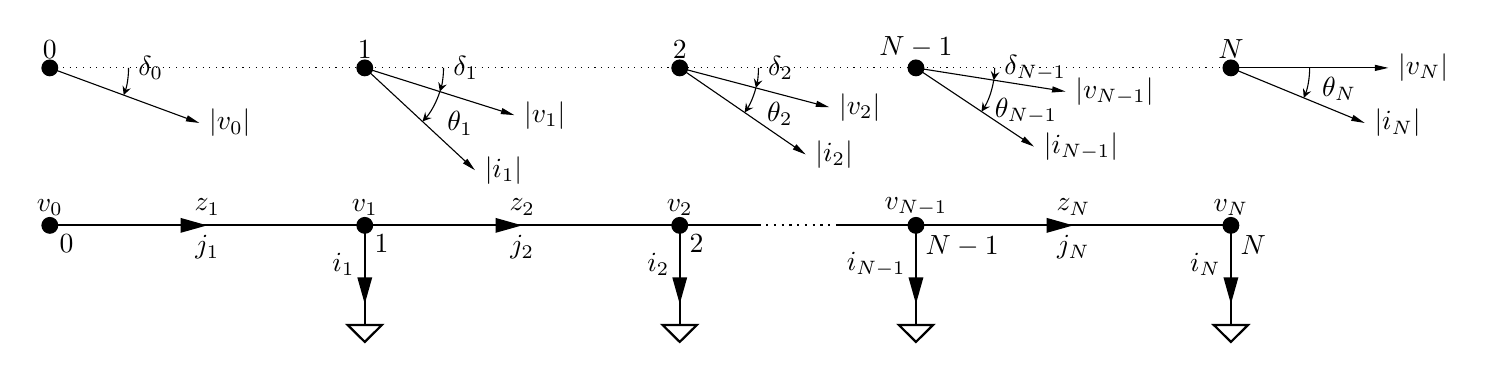
\begin{tikzpicture}
    \draw[fill] (0,0) circle [radius=0.1] node[above]{$v_{0}$} node[below right]{$0$};
    \draw[thick] (0,0) -- (9,0) node[pos=2/9, above]{$z_{1}$} node[pos=6/9, above]{$z_{2}$};
    \draw[arrows = {-Stealth[inset=0pt, angle=30:10pt]}, thick] (0,0) -- (2,0)  node[below]{$j_{1}$};
    \draw[fill] (4,0) circle [radius=0.1] node[above]{$v_{1}$} node[below right]{$1$};
    \draw[arrows = {-Stealth[inset=0pt, angle=30:10pt]}, thick] (4,0) -- (6,0)  node[below]{$j_{2}$};
    \draw[arrows = {-Stealth[fill=none, inset=0pt, angle=90:10pt]}, thick] (4,0) -- (4,-1.5);
    \draw[arrows = {-Stealth[inset=0pt, angle=30:10pt]}, thick] (4,0) -- node[left]{$i_{1}$}(4,-1);
    \draw[fill] (8,0) circle [radius=0.1] node[above]{$v_{2}$} node[below right]{$2$};
    \draw[arrows = {-Stealth[fill=none, inset=0pt, angle=90:10pt]}, thick] (8,0) -- (8,-1.5);
    \draw[arrows = {-Stealth[inset=0pt, angle=30:10pt]}, thick] (8,0) -- node[left]{$i_{2}$}(8,-1);
    \draw[dotted, thick] (9,0) -- (10,0);
    \draw[thick] (10,0) -- (11,0);
    \draw[fill] (11,0) circle [radius=0.1] node[above]{$v_{N-1}$} node[below right]{$N-1$};
    \draw[arrows = {-Stealth[fill=none, inset=0pt, angle=90:10pt]}, thick] (11,0) -- (11,-1.5);
    \draw[arrows = {-Stealth[inset=0pt, angle=30:10pt]}, thick] (11,0) -- node[left]{$i_{N-1}$}(11,-1);
    \draw[thick] (11,0) -- node[above]{$z_{N}$}(15,0);
    \draw[fill] (15,0) circle [radius=0.1] node[above]{$v_{N}$} node[below right]{$N$};
    \draw[arrows = {-Stealth[inset=0pt, angle=30:10pt]}, thick] (11,0) -- (13,0)  node[below]{$j_{N}$};
    \draw[arrows = {-Stealth[fill=none, inset=0pt, angle=90:10pt]}, thick] (15,0) -- (15,-1.5);
    \draw[arrows = {-Stealth[inset=0pt, angle=30:10pt]}, thick] (15,0) -- node[left]{$i_{N}$}(15,-1);

    \draw[dotted, thin] (0, 2) -- (17,2);
    \draw[fill] (0,2) circle [radius=0.1] node[above]{$0$};
    \draw[fill] (4,2) circle [radius=0.1] node[above]{$1$};
    \draw[fill] (8,2) circle [radius=0.1] node[above]{$2$};
    \draw[fill] (11,2) circle [radius=0.1] node[above]{$N-1$};
    \draw[fill] (15,2) circle [radius=0.1] node[above]{$N$};

    \coordinate (a1) at (0,2);
    \coordinate (b1) at (2,2);
    \coordinate (c1) at (1.9,1.3);
    \draw[arrows = {-Stealth[inset=0pt, angle=25:5pt]}] (a1) node[right = 1cm]{$\delta_{0}$}--(c1) node[right]{$|v_0|$};
    \pic[draw,<-,>=stealth,angle eccentricity=1.3, angle radius=1cm] {angle=c1--a1--b1};

    \coordinate (a2) at (4,2);
    \coordinate (b2) at (6,2);
    \coordinate (c2) at (5.9,1.4);
    \coordinate (d2) at (5.4,0.7);
    \draw[arrows = {-Stealth[inset=0pt, angle=25:5pt]}] (a2) node[right = 1cm]{$\delta_{1}$}--(c2) node[right]{$|v_1|$};
    \pic[draw,<-,>=stealth,angle eccentricity=1.3, angle radius=1cm] {angle=c2--a2--b2};
    \draw[arrows = {-Stealth[inset=0pt, angle=25:5pt]}] (a2) -- (d2) node[right]{$|i_1|$};
    \pic["$\theta_1$", draw,<-,>=stealth,angle eccentricity=1.4, angle radius=1cm] {angle=d2--a2--c2};

    \coordinate (a3) at (8,2);
    \coordinate (b3) at (10,2);
    \coordinate (c3) at (9.9,1.5);
    \coordinate (d3) at (9.6,0.9);
    \draw[arrows = {-Stealth[inset=0pt, angle=25:5pt]}] (a3) node[right = 1cm]{$\delta_{2}$}--(c3) node[right]{$|v_2|$};
    \pic[draw,<-,>=stealth,angle eccentricity=1.3, angle radius=1cm] {angle=c3--a3--b3};
    \draw[arrows = {-Stealth[inset=0pt, angle=25:5pt]}] (a3) -- (d3) node[right]{$|i_2|$};
    \pic["$\theta_2$", draw,<-,>=stealth,angle eccentricity=1.4, angle radius=1cm] {angle=d3--a3--c3};

    \coordinate (aN-1) at (11,2);
    \coordinate (bN-1) at (13,2);
    \coordinate (cN-1) at (12.9,1.7);
    \coordinate (dN-1) at (12.5,1);
    \draw[arrows = {-Stealth[inset=0pt, angle=25:5pt]}] (aN-1) node[right = 1cm]{$\delta_{N-1}$}--(cN-1) node[right]{$|v_{N-1}|$};
    \pic[draw,<-,>=stealth,angle eccentricity=1.6, angle radius=1cm] {angle=cN-1--aN-1--bN-1};
    \draw[arrows = {-Stealth[inset=0pt, angle=25:5pt]}] (aN-1) -- (dN-1) node[right]{$|i_{N-1}|$};
    \pic["$\theta_{N-1}$", draw,<-,>=stealth,angle eccentricity=1.5, angle radius=1cm] {angle=dN-1--aN-1--cN-1};

    \coordinate (aN) at (15,2);
    \coordinate (bN) at (17,2);
    \coordinate (cN) at (16.7,1.3);
    \draw[arrows = {-Stealth[inset=0pt, angle=25:5pt]}] (aN)--(bN) node[right]{$|v_N|$};
    \draw[arrows = {-Stealth[inset=0pt, angle=25:5pt]}] (aN) -- (cN) node[right]{$|i_N|$};
    \pic["$\theta_N$", draw,<-,>=stealth,angle eccentricity=1.4, angle radius=1cm] {angle=cN--aN--bN};

  \end{tikzpicture}
  \caption{Bottom: model of a single-phase linear low-voltage distribution feeder. 
  Top: global voltage ($v^g_n$) and current ($i_{n}e^{i\delta_n}$) phasors at each node. In this figure the phase reference is chosen with respect to the last node $N$.}
  \label{f1}
\end{figure*}

The following conventions are used for description of a low-voltage network:
\begin{itemize}
  \item Node $0$ represents a substation transformer.
  \item Linear feeder nodes and lines are indexed such that $n$-th power line connects nodes $n-1$ and $n$, we denote it as $(n-1, n)$. Therefore all linear feeder parameters have one index.
  \item A radial power network is represented by a tree graph $G(\mathcal{N}, \mathcal{E})$ where each node in $\mathcal{N}$ denotes a bus number and each link $(k, n) \in \mathcal{E}$ denotes a power line between nodes $k$ and $n$. Power line related parameters in the radial network require two indices.
  \item We limit our study to steady state behaviour of a single phase LV grid, when all voltages and currents can be represented as phasors.
  \item Small Latin letters are used for complex or real scalars, i.e. $a_n = |a_n|e^{i\angle a_n}$ where $|a_n|$ - amplitude of the complex scalar $a_n$ and $\angle a_n$ - its angle. Bold letters are used for vectors ($\bm{a}_n = \big[a_{1, 1}, \ldots, a_{M, n}\big]^T = \big[a_{1:M, n}\big]^T$) and bold capital letters for matrices ($\bm{A}_n = \big[a_{1:M, 1:N}\big] = \big[\bm{a}_{1:N}\big]$). 
\end{itemize}

\subsection{Linear feeder. Models} 

Consider a single phase model of a linear low-voltage distribution feeder (Fig. \ref{f1}) where $N$ buses (nodes $1, \ldots, N$) are connected in series to a distribution transformer (node $0$). Every bus $n$ has voltage $v_n$ and current $i_n$, that are represented as phasors with angle $\theta_n$ between them. When $\theta_n > 0$, current is lagging the voltage. Power line impedances and corresponding line currents are denoted by $z_n$ and $j_n$ respectively. By $\delta_n$ we denote the phase of a voltage phasor with respect to a global reference, for example in Figure \ref{f1} the phase reference is chosen with respect to the last node $N$.

Throughout this paper we distinguish between global variables, i.e. variables defined with respect to a global phase reference, and local variables, i.e. variables that do not contain global phase angle ($\delta_n$) information:

\begin{itemize}
  \item $v_n \coloneqq |v_n|$ - local voltage at the node $n$;
  \item $v_n^g \coloneqq |v_n|e^{i\delta_n}$ - global voltage at the node $n$;
  \item $i_{n} \coloneqq |i_{n}|e^{i\theta_n}$ - local current (consumed or injected) at the node $n$;
  \item $i^g_{n} \coloneqq |i_{n}|e^{i(\theta_n + \delta_n)} = i_{n}e^{i\delta_n}$ - global current (consumed or injected) at the node $n$;
\end{itemize}

Given only local information $v_n, i_n, \theta_n, z_n$ for all nodes $n$, we can calculate unknown node phases $\delta_n$ and line currents $j_n$ using Propositions \ref{backward_prop} and \ref{forward-prop}. 

\begin{proposition}[Backward model]
  Refer to Fig. \ref{f1}. Let the phase reference be chosen with respect to the last node $N$ (as in Fig. \ref{f1}), i.e. $\delta_N = 0$. Also, let $j_{n} \coloneqq |j_{n}|e^{i\beta_n}$ is a local line current, then
  \begin{equation}
    \begin{split}
    v_{n-1}e^{i\Delta_{n}} - v_{n} = j_{n}z_{n}, \\
    j_{n-1} = i_{n-1} + j_{n}e^{-i\Delta_{n}}
    \end{split}
    \label{l_pi_original}
  \end{equation}
  for all $n$, where $\Delta_{n} = \delta_{n-1} - \delta_{n}$ is the phase increment corresponding to the power line $(n-1, n)$. 
  \label{backward_prop}
\end{proposition}

\begin{proof}
Define a global line current, flowing between nodes $n-1$ and $n$ as $j^{g}_{n} \coloneqq j_{n}e^{i\delta_n} = |j_{n}|e^{i(\beta_n + \delta_n)}$, i.e. its phase is calculated with respect to the (receiving) node $n$, which gives $j^{g}_{N} = i_N$. Using Ohm's law, we can find the ($N-1$)-th node's phase $\delta_{N-1}$: 
  $$v_{N-1}e^{i\delta_{N-1}} - v_{N} = j^{g}_{N}z_{N},$$
and from Kirchoff's current law we calculate current $j^{g}_{N-1} = i^g_{N-1} + j^{g}_{N}$ flowing between nodes $N-1$ and $N$.
We repeat this procedure for nodes $N-2, N-3, \ldots, 0$, find all phases and obtain the following recursive relations for phases and line currents in the feeder:
\begin{equation*}
  \begin{split}
  v_{n-1}e^{i\delta_{n-1}} - v_{n}e^{i\delta_n} = j^{g}_{n}z_{n}, \\
  j^{g}_{n-1} = i^g_{n-1} + j^{g}_{n}.
  \end{split}
\end{equation*}
Divide the first equation by $e^{i\delta_{n}}$, the second by $e^{i\delta_{n-1}}$, and then noting that $j^{g}_n e^{-i\delta_n} = j_n$, we obtain the model (\ref{l_pi_original}) written in terms of phase increments and local variables.
\end{proof}

It is often convenient to choose the phase reference with respect to the distribution transformer which leads to the alternative model. 
\begin{proposition}[Forward model]
  Refer to Fig. \ref{f1}. Let the phase reference be chosen with respect to the first node in the network, i.e. $\delta_0 = 0$. Also, let $j_{n} \coloneqq |j_{n}|e^{i\phi_n}$ is a local line current, then
  \begin{equation}
    \begin{split}
    v_{n-1} - v_{n}e^{-i\Delta_{n}} = j_{n}z_{n}, \\
    j_{n+1} = j_{n}e^{i\Delta_{n}} - i_{n}
    \end{split}
    \label{lf-forward1}
  \end{equation}
  for all $n$, where $\Delta_{n} = \delta_{n-1} - \delta_{n}$ is the phase increment corresponding to the power line $(n-1, n)$. 
  \label{forward-prop}
\end{proposition}

\begin{proof}
  Define a global line current as $j^{g}_{n} \coloneqq j_{n}e^{i\delta_{n-1}} = |j_{n}|e^{i(\phi_n + \delta_{n-1})}$ , i.e. its phase is defined with respect to the (sending) node $n-1$. This definition enables us to start consideration from the first node of the linear feeder, where $\delta_0 = 0$. Following the same procedure as in the proof of Proposition \ref{backward_prop} we obtain:
  \begin{equation*}
    \begin{split}
    v_{n-1}e^{i\delta_{n-1}} - v_{n}e^{i\delta_n} = j^{g}_{n}z_{n}, \\
    j^{g}_{n+1} = j^{g}_{n} - i^g_{n}.
    \end{split}
  \end{equation*}
  Divide the first equation by $\delta_{n-1}$ and the second one by $\delta_{n}$ we get a model (\ref{lf-forward1}) written in terms of phase increments and local variables. 
\end{proof}

\begin{remark} \hfill
\begin{itemize}
  \begin{comment}
  \item Another useful forward model formulation is obtained after excluding the phase term $e^{i\Delta_{n}}$:
        \begin{equation}
        \begin{split}
        |v_{n-1}| - |v_{n}|e^{-i\Delta_{n}} = j_{n}z_{n} \\
        j_{n+1} = j_{n}\frac{|v_{n-1}|}{|v_{n}|} - z_{n}^*\frac{|j_{n}|^2}{|v_{n}|} - i_{n}
        \end{split}
        \label{lf-forward2}
        \end{equation}
  \end{comment}
  \item The forward model has some limitations. For instance, it requires knowledge of the substation transformer current (i.e. $j_{1}$ on fig. \ref{f1}). In the context of impedance identification this means that its magnitude and phase should be known from measurements. However, this is not always the case for LV distribution grids. Another limitation will become apparent when considering the tree network case. 
  \item The forward and backward models are essentially equivalent in that the forward model (\ref{lf-forward1}) can be obtained from (\ref{l_pi_original}) by multiplying the first equation by $e^{-i\Delta_{n}}$ and noting the difference in phases for line current definitions.  
\end{itemize} 
\end{remark}

\subsection{Tree network}{}

The results of the previous subsection can be extended to the case of a tree topology. We start from a simple branching example, show how to resolve it using the system of equations (\ref{l_pi_original}) and then generalise this approach for any tree network.
\begin{proposition}
  The backward model (\ref{l_pi_original}) resolves any network with tree topology.
\end{proposition}{}
\begin{proof}[Proof (Outline)]
  Consider the network topology case depicted on Fig. \ref{f2} which consists of three buses{} connected in the form of the simplest branching.
  \begin{figure}[H]
  \centering
  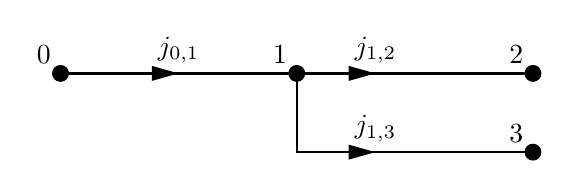
\begin{tikzpicture}
  \draw[fill] (0, 0) circle [radius=0.1] node[above left]{$0$};
  \draw[thick] (0, 0) -- (3, 0);
  \draw[arrows = {-Stealth[inset=0pt, angle=30:10pt]}, thick] (0,0) -- (1.5,0)  node[above]{$j_{0,1}$};
  \draw[fill] (3, 0) circle [radius=0.1] node[above left]{$1$};
  %\draw[arrows = {-Stealth[fill=none, inset=0pt, angle=90:10pt]}, thick] (3, 0) -- (3, -2);
  %\draw[arrows = {-Stealth[inset=0pt, angle=30:10pt]}, thick] (3,0) -- (3, -1)  node[right]{$i_{1}$};
  \draw[thick] (3, 0) -- (6, 0);
  \draw[fill] (6, 0) circle [radius=0.1] node[above left]{$2$};
  %\draw[arrows = {-Stealth[fill=none, inset=0pt, angle=90:10pt]}, thick] (6,0) -- (6,-2);
  %\draw[arrows = {-Stealth[inset=0pt, angle=30:10pt]}, thick] (6,0) -- (6, -1)  node[right]{$i_{2}$};
  \draw[arrows = {-Stealth[inset=0pt, angle=30:10pt]}, thick] (3,0) -- (4, 0)  node[above]{$j_{1,2}$};
  \draw[thick] (3, 0) -- (3, -1) -- (6, -1);
  \draw[fill] (6, -1) circle [radius=0.1] node[above left]{$3$};
  %\draw[thick] (3, 2) -- (2, 2);
  %\draw[arrows = {-Stealth[inset=0pt, angle=30:10pt]}, ultra thick, dotted] (6.5,1) -- (5,1)  node[pos=1/2, above]{\textbf{BCI}$_1$};
  %\draw[arrows = {-Stealth[inset=0pt, angle=30:10pt]}, ultra thick, dotted] (4,2.5) -- (4,1)  node[pos=1/2, right]{\textbf{BCI}$_2$};
  %\draw[arrows = {-Stealth[inset=0pt, angle=30:10pt]}, thick] (3, 2) -- (2, 2)  node[above]{$i_{3}$};
  %\draw[arrows = {-Stealth[fill=none, inset=0pt, angle=90:10pt]}, thick] (2, 2) -- (2, 1);
  \draw[arrows = {-Stealth[inset=0pt, angle=30:10pt]}, thick] (3, -1) -- (4, -1) node[above]{$j_{1,3}$};
  %\draw[dotted, thick] (6, 0) -- (6.5, 0);
  %\draw[dotted, thick] (3, 2) -- (3, 2.5);
  \end{tikzpicture}
  \caption{The simplest branching case}
  \label{f2}
  \end{figure}
  Apply backward model (\ref{l_pi_original}) to branches $(1, 3)$ and $(1, 2)$ simultaneously and find $\Delta_{1,3}$, $\Delta_{1,2}$, $j_{0, 1}$:
  \begin{equation}
    \begin{split}
      &{} v_{1}e^{i\Delta_{1,3}} - v_{3} = j_{1,3}z_{1,3}, \\
      & v_{1}e^{i\Delta_{1,2}} - v_{2} = j_{1,2}z_{1,2},
    \end{split}
  \end{equation}
  where $j_{1,3} = i_3$ and $j_{1,2} = i_2$. Then 
  $$j_{0, 1} = j_{0, 1}^ge^{-i\delta_{1}} = j_{1,3}e^{-i\Delta_{1,3}} + j_{1,2}e^{-i\Delta_{1,2}} + i_1.$$
  Next, we choose the global phase reference and find absolute values of phases at every point in the network. Without loss of generality we can pick $\delta_2 = 0$, which gives $\delta_1 = \Delta_{1,2}$. Therefore, using the definition of the phase increment introduced earlier, $\delta = [\delta_0, \delta_1, \delta_3]^T$ can be found from the following system of linear equations:
  \begin{equation*}
  \begin{bmatrix}
  \Delta_{0,1} \\
  \Delta_{1,2} \\
  \Delta_{1,3}
  \end{bmatrix} = 
  \begin{bmatrix}
  1 & -1 & 0 \\
  0 & 1 & 0 \\
  0 & 1 & -1  
  \end{bmatrix}
  \begin{bmatrix}
  \delta_{0} \\
  \delta_{1} \\
  \delta_{3} 
  \end{bmatrix}.
  \end{equation*}
  The same calculation can be immediately generalised to the case when node $1$ has $n > 2$ links:
  \begin{equation*}
  \begin{bmatrix}
  \Delta_{0,1} \\
  \Delta_{1,2} \\
  \vdots \\
  \Delta_{1,n-1} \\
  \Delta_{1,n}
  \end{bmatrix} = 
  \begin{bmatrix}
  1 & -1 & 0 & \ldots & 0 & 0 \\
  0 & 1 & 0 & \ldots & 0 & 0 \\
  \vdots & \vdots & \vdots & \ddots & \vdots & \vdots \\
  0 & 1 & 0 & \ldots & -1 & 0 \\
  0 & 1 & 0 & \ldots & 0 & -1 \\
  \end{bmatrix}
  \begin{bmatrix}
  \delta_{0} \\
  \delta_{1} \\
  \vdots \\
  \delta_{n-1} \\
  \delta_{n}
  \end{bmatrix}.
  \end{equation*}
  It is known from graph theory, that for any tree graph the number of vertices is equal to the number of branches minus one \cite[Corollary $1.5.3$]{diestel2005graph}, i.e. for any tree graph $G(\mathcal{N}, \mathcal{E})$ with number of nodes/vertices $|\mathcal{N}|$ and 
  number of branches $|\mathcal{E}|$, $|\mathcal{N}| = |\mathcal{E}| - 1.$
  Thus any tree can be iteratively constructed by adding a pair consisting of a vertex and branch, which shows that the above procedure works for a linear feeder as well as for branching with $n$ links, therefore it is applicable for any tree network. 
\end{proof}
\begin{remark} \hfill
\begin{itemize}
  \item The phase matching procedure is required at branching nodes in a tree topology case, as briefly described in the proof above. For the complete algorithm refer to Algorithm \ref{phase_matching_procedure} in Section \ref{system_identification_section}.
  \item The forward model (\ref{lf-forward1}) is more cumbersome in a branching case. There are additional unknowns that need to be carried until termination. As an example, for the branching on Figure \ref{f2}:
  $$j^g_{0,1} = i_{1}e^{i\Delta_{0, 1}} + j_{1,2}^g + j_{1,3}^g,$$
  currents $j_{1,2}^g$ and $j_{1,3}^g$ are unknown, i.e. there are 2 equations, 4 unknowns.
\end{itemize}
\end{remark}

\subsection{Discussion}

As we saw in the previous sections, the forward model is not well suited to a complete low-voltage network description, hence we use the backward model further in the remainder of this paper. 

To conclude the modelling part we present an iterative model directly based on the backward model (\ref{l_pi_original}) for a single phase low-voltage network that we will exploit for impedance identification purposes. For any node $n$, the set of its ancestors ($\mathcal{A}_n$) and children ($\mathcal{C}_n$) in $G(\mathcal{N}, \mathcal{E})$ obey an iterative relationship:
\begin{equation}
\begin{split}
&{} v_{n}e^{i\Delta_{n, l}} - v_{l} = j_{n, l}z_{n, l}, \quad l \in \mathcal{C}_n,\\
& \sum_{k \in \mathcal{A}_n} j_{k, n} = i_{n} + \sum_{l \in \mathcal{C}_n} j_{n, l}e^{-i\Delta_{n, l}}.
\end{split}
\label{l_pi_general}
\end{equation}
Finally, it is worth noting that the system of equations (\ref{l_pi_general}) is not a new model for power networks. 
\begin{proposition}
  The system of equations (\ref{l_pi_general}) implies the standard power flow model:
  \begin{equation}
    \begin{split}
    &{} v_{n}^2 = v_{l}^2 + S_{n, l}z_{n, l}^* + S_{n, l}^*z_{n, l} + |j_{n, l}^gz_{n, l}|^2, \quad l \in \mathcal{C}_n, \\
    & \sum_{k \in \mathcal{A}_n} S_{k, n} - \sum_{l \in \mathcal{C}_n} (S_{n, l} + |j_{n, l}^g|^2z_{n, l})- s_{n} = 0.
    \end{split}
    \label{bpf_general}
  \end{equation}
  where $S_{n, l} = j_{n, l}^{g*}v_l^g$ and $s_{n} = i^{g*}_{n}v^{g}_{n}$.
\end{proposition}
\begin{proof}
  Exclude the phase term $e^{i\Delta_{n, l}}$ in (\ref{l_pi_general}) and introduce the \textit{receiving-end} \footnote{Note that the sign for terms with $|j_{n, l}|^2$ in resulting power flow equations is reversed with respect to the case when branch power is defined as sending-end complex power flow, i.e. $S_{n, l}=j_{n, l}^*v_n$.} complex power flow from $n$ to $l$ as $S_{n, l}=j_{n, l}^{g*}v_l^g = j_{n, l}^*|v_l|$ (since $ j_{n, l}^{g*}v_l^g = j_{n, l}^*e^{-i\delta_l}|v_l|e^{i\delta_l} = j_{n, l}^*|v_l|$), and  complex power injection $s_{n}$ to obtain:
  \begin{equation*}
    \begin{split}
    &{} v_{n}e^{i\Delta_{n, i}} - v_{i} = j_{n, i}z_{n, i}, \quad i \in \mathcal{C}_n,\\
    & \sum_{k \in \mathcal{A}_n} S_{k, n}^* = s_{n} + \sum_{i \in \mathcal{C}_n} (S_{n, i}^* + |j_{n, i}|^2z_{n, i}^*).
    \end{split}
  \end{equation*}
  Next, transfer the $v_i$ term to the right-hand side, take the magnitude squared of the first equation (also, note that $|j_{n, i}|^2 = |j_{n, i}^g|^2$) and complex conjugate of the second equation to obtain the well known power flow model (\ref{bpf_general}).
\end{proof} 

\begin{remark}
  Comparing equations (\ref{bpf_general}) and (\ref{l_pi_general}), we notice that the impedance term in the power flow model appears as $z_{n, l}$ and $|z_{n, l}|^2$, whereas the backward model has only $z_{n, l}$. Therefore, (\ref{l_pi_general}) is a better conditioned set of equations and we prefer it over (\ref{bpf_general}) for the problem of impedance identification, that we consider in detail in the next section.
\end{remark}

\section{System identification}
\label{system_identification_section}
In this section we consider the problem of system identification, that is, the problem of identifying impedances in a low-voltage network and we develop an approach that exploits the iterative structure of the backward model (\ref{l_pi_general}). We work through the details for a linear feeder model, however the proposed method can be generalised to any tree network as described earlier. We first formulate the optimisation problem for the whole network and then consider two methods to solve it approximately.

We start by considering the same linear feeder model as before (fig. \ref{f1}) with the following measurements available:
\begin{itemize}
  \item $\bm{v}_0$ - RMS \footnote{Root mean square} substation transformer voltage,
  \item $\bm{v}_{n} = \big[ v_{n}^{(1)}, \ldots, v_{n}^{(M)} \big]^T$ - RMS voltage measurements at node $n$,
  \item $|\bm{i}_{n}| = \big[ |i_{n}^{(1)}|, \ldots, |i_{n}^{(M)}| \big]^T$ - RMS consumption current measurements at node $n$, 
  \item $\bm{\theta}_{n} = \big[\theta_{n}^{(1)}, \ldots, \theta_{n}^{(M)}]^T$ - angle measurements between voltage and current phasors,
\end{itemize}
where indices $n = 1:N$ and $m = 1:M$ are used for node and measurement number respectively, e.g. $v_{n}^{(m)}$ - RMS value of the voltage at node $n$ corresponding to the $m$-th measurement\footnote{Although the index $m$ is used for measurement number, it does not necessarily mean that the corresponding quantity is measured, e.g. the value of $j_{n}^{(m)}$ corresponds to $m$-th measurement, but it is not measured directly and must be derived from other measurements.}. According to the minimum functionality requirements for smart metering infrastructure in Australia, every smart meter should be capable of measuring total active power, reactive power and voltage magnitude \cite[Table $6-2$]{SMmin_au}, which is equivalent to availability of $\bm{v}_{n}, |\bm{i}_{n}|, \bm{\theta}_n$ for all $n$. 

Regarding the measurements we assume the following.

\textbf{Assumption 1}. Smart meter measurements can be considered time synchronised with respect to system changes, i.e. for the $m$-th measurement taken from every node, load impedances remain constant. Refer to Fig. \ref{time_synchronicity}.
\begin{figure}[H]
  \centering
  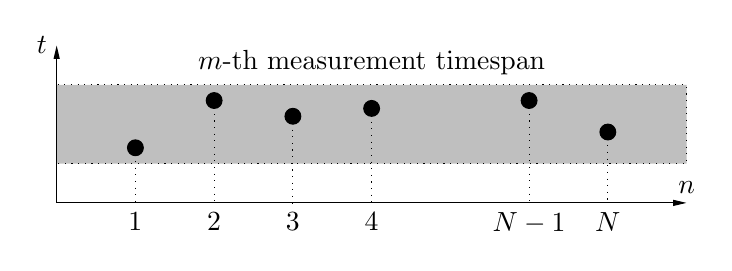
\begin{tikzpicture}
    \coordinate (zero) at (0, 0);
    \coordinate (node_n) at (8, 0);
    \coordinate (tn) at (0, 2);
    \coordinate (g0) at (0, 0.5);
    \coordinate (g1) at (0, 1.5);
    \coordinate (g2) at (8, 1.5);
    \coordinate (g3) at (8, 0.5);
    \draw[dotted, thin, fill=gray!50] (g0)--(g1)--node[above]{$m$-th measurement timespan}(g2)--(g3)--(g0);
    \draw[arrows = {-Stealth[inset=0pt, angle=25:5pt]}] (zero) -- (node_n) node[above]{$n$};
    \draw[arrows = {-Stealth[inset=0pt, angle=25:5pt]}] (zero) -- (tn) node[left]{$t$};

    % dot coordinates
    \coordinate (d0) at (1, 0.7);
    \coordinate (d0p) at (1, 0);
    \coordinate (d1) at (2, 1.3);
    \coordinate (d1p) at (2, 0);
    \coordinate (d2) at (3, 1.1);
    \coordinate (d2p) at (3, 0);
    \coordinate (d3) at (4, 1.2);
    \coordinate (d3p) at (4, 0);
    \coordinate (d4) at (6, 1.3);
    \coordinate (d4p) at (6, 0);
    \coordinate (d5) at (7, 0.9);
    \coordinate (d5p) at (7, 0);

    \draw[fill] (d0) circle [radius=0.1]; \draw[dotted] (d0) -- (d0p)node[below]{$1$};
    \draw[fill] (d1) circle [radius=0.1]; \draw[dotted] (d1) -- (d1p)node[below]{$2$};
    \draw[fill] (d2) circle [radius=0.1]; \draw[dotted] (d2) -- (d2p)node[below]{$3$};
    \draw[fill] (d3) circle [radius=0.1]; \draw[dotted] (d3) -- (d3p)node[below]{$4$};
    \draw[fill] (d4) circle [radius=0.1]; \draw[dotted] (d4) -- (d4p)node[below]{$N-1$};
    \draw[fill] (d5) circle [radius=0.1]; \draw[dotted] (d5) -- (d5p)node[below]{$N$};
  \end{tikzpicture}
  \caption{Time synchronicity assumption. Gray region is a single time stamp corresponding to $m$-th measurement.}
  \label{time_synchronicity}
\end{figure}
This is justified because smart metering minimum functionality specifications require smart meters to maintain measurement time clocks to within a few seconds across a network, see e.g. \cite[Chapter $7.5$]{SMmin_au},\cite[Chapter $6$]{NMI_au}. 
\begin{remark}
Importantly, the smart meter measurements are not phase synchronous and phase synchronicity is not needed for our algorithms. Figure \ref{f3} shows the difference between phase and time synchronicity for measurements in phasor representation.
\end{remark}
\begin{figure}[H]
  \centering
  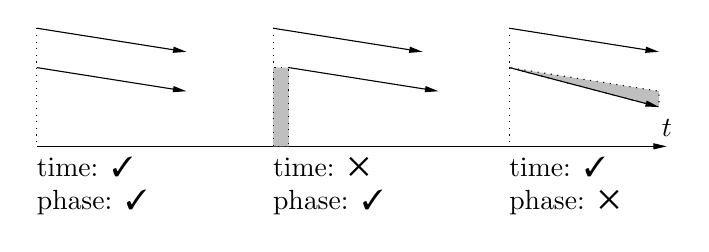
\begin{tikzpicture}
    \coordinate (t0) at (0, 0.5);
    \coordinate (tn) at (8, 0.5);
    \draw[arrows = {-Stealth[inset=0pt, angle=25:5pt]}] (t0) -- (tn) node[above]{$t$};

    % arrows 1
    \coordinate (a1) at (0, 2);
    \coordinate (c1) at (1.9, 1.7);
    \draw[arrows = {-Stealth[inset=0pt, angle=25:5pt]}] (a1) -- (c1);
    \draw[thin, dotted](a1) -- (0, 0.5);

    \coordinate (a2) at (0,1.5);
    \coordinate (c2_) at (1.9, 1.2);
    \coordinate (c2) at (1.9, 1);
    %\draw[dotted, thin, fill=gray!50] (a2)--(c2)--(c2_)--(a2);
    \draw[arrows = {-Stealth[inset=0pt, angle=25:5pt]}] (a2) -- (c2_);

    \coordinate (text1) at (1, 0);
    \node[text width=2cm] at (text1){time: \cmark \\ phase: \cmark};

    % arrows 2
    \coordinate (a3) at (3,2);
    \coordinate (c3) at (4.9,1.7);
    \draw[arrows = {-Stealth[inset=0pt, angle=25:5pt]}] (a3) -- (c3);
    \draw[thin, dotted](a3) -- (3, 1.5);

    \coordinate (a4) at (3, 1.5);
    \coordinate (a4_) at (3.2, 1.5);
    \coordinate (c4) at (5.1, 1.2);
    \draw[dotted, thin, fill=gray!50] (a4_)--(a4)--(3, 0.5)--(3.2, 0.5)--(a4_);
    \draw[arrows = {-Stealth[inset=0pt, angle=25:5pt]}] (a4_) -- (c4);

    \coordinate (text2) at (4, 0);
    \node[text width=2cm] at (text2){time: \xmark \\ phase: \cmark};

    % arrows 3
    \coordinate (a5) at (6,2);
    \coordinate (c5) at (7.9,1.7);
    \draw[arrows = {-Stealth[inset=0pt, angle=25:5pt]}] (a5) -- (c5);
    \draw[thin, dotted](a5) -- (6, 0.5);

    \coordinate (a6) at (6,1.5);
    \coordinate (c6_) at (7.9, 1.2);
    \coordinate (c6) at (7.9, 1);
    \draw[dotted, thin, fill=gray!50] (a6)--(c6)--(c6_)--(a6);
    \draw[arrows = {-Stealth[inset=0pt, angle=25:5pt]}] (a6) -- (c6);

    \coordinate (text3) at (7, 0);
    \node[text width=2cm] at (text3){time: \cmark \\ phase: \xmark};
  \end{tikzpicture}
  \caption{Difference between phase and time synchronicity of measurements. Phasor representation.}
  \label{f3}
\end{figure}
\textbf{Assumption 2} Line impedances and grid topology remain unchanged during the whole measurement process. 
\begin{remark} 
Algorithms that we develop in the next section allow us to monitor varying line impedances and, therefore, detect topology changes.
\end{remark}
\textbf{Assumption 3}. Smart meter measurement uncertainty is approximated by Gaussian noise $\mathcal{N}(0, \sigma)$, where $\sigma$ corresponds to $1\%$ full scale error which is practical for the majority of household smart meters, see e.g. technical reports \cite[Chapter $4$]{NMI_au}, \cite[Chapter $7.1$]{SMmin_au}.
\begin{remark}
  Note, however, that $1\%$ of full scale error for voltage, current and angle corresponds to about $2\%$ error in measured power, i.e. this setup can be considered as a worst case. Thus, we also consider $0.5\%$ and $0.1\%$ of full scale error cases.
\end{remark}

\subsection{Problem formulation. Linear feeder}

Consider a linear feeder (Fig. \ref{f1}) and formulate the problem of identifying impedances based on the backward model (\ref{l_pi_original}) written in multidimensional form (i.e. when multiple measurements are gathered):
\begin{equation}
\begin{split}
&{} \bm{v}_{n-1}e^{i\bm{\Delta}_{n}} - \bm{v}_{n} = \bm{j}_{n}z_{n}, \\
& \bm{j}_{n-1} = \bm{i}_{n-1} + \bm{j}_{n}e^{-i\bm{\Delta}_{n}},
\end{split}
\label{lf-sysid-model}
\end{equation}
where $\bm{v}_{n} = \big[ v^{(1)}_{n}, \ldots, v^{(M)}_{n} \big]^T$, $\bm{j}_{n} = \big[ j^{(1)}_{n}, \ldots, j^{(M)}_{n} \big]^T$, $\bm{\Delta_n} = \big[ \Delta^{(1)}_{n}, \ldots, \Delta^{(M)}_{n} \big]^T$ and $e^{i\bm{\Delta}_{n}}$ is a component-wise operation as well as multiplication of two vectors $\bm{v}_{n-1}e^{i\bm{\Delta}_{n}}$ and $\bm{j}_{n}e^{i\bm{\Delta}_{n}}$.

Next, define a cost function for the $n$-th power line based on the first equation in (\ref{lf-sysid-model}): 
\begin{equation}
c_n(z_{n}, \bm{j}_n, \bm{\Delta}_{n}) = \Big\| \bm{v}_{n-1}e^{i\bm{\Delta}_{n}} - \bm{v}_{n} - \bm{j}_{n}z_{n} \Big\|_2^2,
\label{cost_function}
\end{equation} 
and introduce a cost-to-go function
\begin{equation}
J_{k:N} = \sum_{n = k}^{N} c_n(z_{n}, \bm{j}_n, \bm{\Delta}_{n})
\label{total_cost}
\end{equation}
for lines $N, N-1, \ldots, k$. Using the second equation in (\ref{lf-sysid-model}) we formulate the problem of impedance identification in a linear feeder:
\begin{equation}
\begin{aligned}
& \minimise_{z_{1:N}, \bm{\Delta}_{0:N-1}}
& & J_{1:N} \\
& \st
& & \bm{j}_{n-1} = \bm{i}_{n-1} + \bm{j}_{n}e^{-i\bm{\Delta}_{n}}, \\
&&& \bm{j}_{N} = \bm{i}_{N}, \\
&&& n = 1,\ldots, N-1.
\end{aligned}
\label{pf_network}
\end{equation}
The resulting optimisation problem is non-linear and non-convex. In the next subsections we consider simplifications that allow solution for different practical scenarios.

\subsection{Identification algorithm. Linearised case}

The first simplification is based on the following assumption.

\textbf{Assumption 4} The phase increments $\Delta_n$ are negligibly small. 

To justify this, consider the backward model (\ref{l_pi_original}) and take the imaginary part of the first equation: 
$\sin{\Delta_{n}} = \frac{\Imag{(j_{n}z_{n})}}{|v_{n-1}|} \le \frac{|j_{n}z_{n}|}{|v_{n-1}|}.$
Thus, the value of the phase increment is bounded by the voltage drop of the corresponding power line, which is a very small quantity for low-voltage networks due to short length (up to a few hundred meters) of the power lines.
\begin{remark}
Note, that we neglect the phase increments but we do not neglect the absolute phase at each node in the network. 
\end{remark}
Under Assumption 3, the model (\ref{lf-sysid-model}) takes the form:
\begin{equation}
  \begin{split}
  \bm{v}_{n-1} - \bm{v}_{n} = \bm{j}_{n}z_{n}, \\
  \bm{j}_{n-1} = \bm{i}_{n-1} + \bm{j}_{n}.
  \end{split}
  \label{lf-sysid-model-lin}
\end{equation}
Then the cost function (\ref{cost_function}) can be linearised and rewritten as follows by splitting it into real and imaginary parts:
\begin{equation}
  c^{l}_n(\bm{z}_{n}, \bm{j}_n) = \Big\| \bm{v}_{n-1} - \bm{v}_{n} - \bm{J}_{n}\bm{Q}_1\bm{z}_{n} \Big\|_2^2 + \Big\|\bm{J}_{n}\bm{Q}_2\bm{z}_{n} \Big\|_2^2,
  \label{cost_function-lin}
\end{equation}
where $\bm{J}_n \coloneqq \big[ \Real{\bm{j}_n} \quad \Imag{\bm{j}_n}\big]$, $\bm{z}_n \coloneqq \big[ \Real{z_n} \quad \Imag{z_n} \big]^T$, $\bm{Q}_1 \coloneqq 
\begin{bmatrix}
1 & 0 \\
0 & -1
\end{bmatrix}$ and $\bm{Q}_2 \coloneqq
\begin{bmatrix}
0 & 1 \\
1 & 0
\end{bmatrix}$.
Therefore, we obtain the optimisation problem of the form:
\begin{equation}
  \begin{aligned}
  & \minimise_{\bm{z}_{1:N}} 
  & & J^l_{1:N} \\
  & \st
  & & \bm{j}_{n-1} = \bm{i}_{n-1} + \bm{j}_{n}, \\
  &&& \bm{j}_{N} = \bm{i}_{N}, \\
  &&& n = 1,\ldots, N-1.
  \end{aligned}
  \label{lf-sysid-problem-lin}
\end{equation}
where $J^l_{1:N} = \sum_{n = 1}^{N} c^l_n(\bm{z}_{n}, \bm{j}_n)$ is the corresponding linearised cost-to-go function. The following proposition shows how this problem can be further simplified.
\begin{proposition}
Minimising the sum in (\ref{lf-sysid-problem-lin}) is equivalent to minimising each term $c^l_n(\bm{z}_{n}, \bm{j}_n)$ separately.
\end{proposition}
\begin{proof}
  To show this, consider the cost-to-go function for the last two power lines:
  \begin{equation*}
    \begin{split}
    &{}J_{N-1:N} = \min_{\bm{z}_{N-1:N}} \big[ c^l_{N-1}(\bm{z}_{N-1}, \bm{j}_{N-1}) + c^l_N(\bm{z}_{N}, \bm{j}_{N}) \big] = \\
    & = \min_{\bm{z}_{N-1}} \big[ c_{N-1}(\bm{z}_{N-1}, \bm{i_{N-1}} + \bm{j}_{N}) \big] + \min_{\bm{z}_{N}} \big[ c^l_N(\bm{z}_{N}, \bm{j}_{N}) \big],
    \end{split}
  \end{equation*}
  where both terms are the impedance identification problems for lines $N$ and $N-1$. Using the same argument for $N$ power lines, we conclude that minimising sum in (\ref{pf_network}) is equivalent to minimising each term separately.
\end{proof}
\begin{remark}
\hfill
\begin{itemize}
  \item Minimisation of $c^l_n(\bm{z}_n, \bm{j}_n)$ with respect to $\bm{z}_n$ is a simple unconstrained least squares problem, where the second term can be interpreted as a regularisation term. Note, that it appears naturally in the problem formulation.
  \item Formally, measurement noise affects the $\bm{J}_n$ term, since it contains data (real and imaginary parts of $\bm{j}_n$) derived from measurements. In practice, the main source of error is the voltage measurement noise, therefore the error in matrix $\bm{J}_n$ can be neglected in favour of using a linear least squares approach. Linear least squares estimation is also preferable as a simple (from a computational perspective for decentralised implementation) and flexible (i.e. has recursive, weighted modifications) method. This allows real-time tracking of impedances in the network as new measurements become available. Nevertheless, when errors in $\bm{J}_n$ need to be taken into account, total least squares (TLS) techniques can be used \cite{golub1999tikhonov}.
\end{itemize}
\end{remark}
As a result, we obtain the algorithm that solves problem (\ref{lf-sysid-problem-lin}). Since it identifies the network starting from the edge node and propagating all the way through to the first node, we call it LBCI (Linearised Backward Calculation of Impedances):
\begin{algorithm}[H]
\caption{LBCI algorithm for a linear feeder}
\label{a2}
\begin{algorithmic}[1]
\State $\mathcal{M} \coloneqq \{\bm{v}_{n}, |\bm{i}_{n}|, \bm{\theta}_{n} ~\big|~ n=1, \ldots, N \} \cup \{ \bm{v}_0 \}$
\Function{LBCI}{$\mathcal{M}$}
\State $\bm{j}_{N} = \bm{i}_{N}$
\For{$n = N : 1$}
\State $\widehat{\bm{z}}_n = \argmin_{\bm{z}_{n}} c^{l}_n(\bm{z}_{n}, \bm{j}_n)$
\State $\bm{j}_{n-1} = \bm{i}_{n-1} + \bm{j}_{n}$
\EndFor
\State \Return $\widehat{\bm{Z}} = \big[ \widehat{\bm{z}}_{1:N} \big], \bm{J} = \big[ \bm{j}_{1:N} \big]$
\EndFunction
\end{algorithmic}
\end{algorithm} 

Generalisation to a tree topology feeder involves one extra step: we need to keep track of phase increments in order to match the absolute phases of line currents at the intersection point. Note, that because of linearisation we do not obtain correct values of absolute phases, however this is not an issue for identification purposes, since the backward model (\ref{l_pi_original}) is based on the incremental phase information. 

Let $\mathcal{M}^{i}$ and $\mathcal{M}^{j}$ be the sets of measurements for branches $i$ and $j$ that have a common node $n^*$ and sets of indices $\mathcal{N}^i$ and $\mathcal{N}^j$ correspondingly. We briefly summarise the procedure of phase matching:
\begin{algorithm}[H]
\caption{Phase matching procedure}
\label{phase_matching_procedure}
\begin{algorithmic}[1]
%\Require $\mathcal{M}^i$, $\mathcal{M}^j$
\State Calculate: $$\widehat{\bm{Z}}^i, \bm{J}^i =\textproc{LBCI}(\mathcal{M}^i), \quad \widehat{\bm{Z}}^j, \bm{J}^j = \textproc{LBCI}(\mathcal{M}^j).$$
\State For a common node $n^*$ find absolute phases as a sum of phase increments $\bm{\Delta}_{k}$ \footnotemark:
$$\bm{\Delta}_{k} = \frac{\bm{J}_{k}\bm{Q}_2 \widehat{\bm{z}}^i_{k}}{\bm{v}_{k-1}}, \quad \bm{\delta}^i_{n*} \approx \sum_{k \in \mathcal{N}_i} \bm{\Delta}_{k} , \quad \bm{\delta}^j_{n*} \approx \sum_{k \in \mathcal{N}_j} \bm{\Delta}_{k}.$${}
\State Chose $\bm{\delta}^i_{n*}$ as a reference and update phases in branch $j$ by a factor of $\bm{\delta}^i_{n*} - \bm{\delta}^j_{n*}$. This is shown by black arrows in Fig. \ref{f4}.
%\Ensure $\widehat{\bm{Z}} = \big[ \widehat{\bm{z}}_{1:N} \big], \bm{J} = \big[ \bm{j}_{1:N} \big]$
\end{algorithmic}
\end{algorithm}
\footnotetext{Formula for $\bm{\Delta}_{k}$ is obtained from (\ref{lf-sysid-model}) after taking imaginary part of the first equation.}
\begin{figure}[ht]
  \centering
  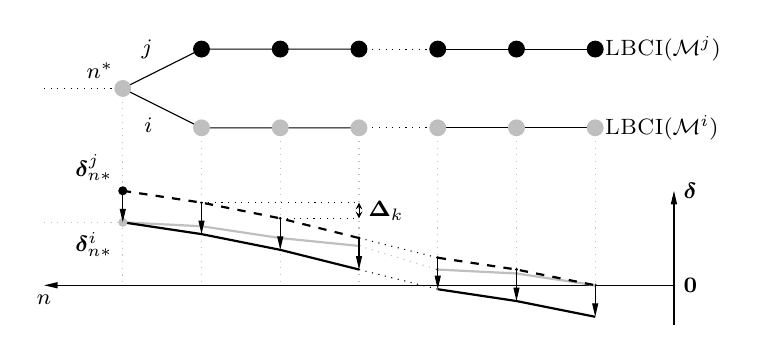
\begin{tikzpicture}
    \coordinate (a0) at (-1, 3);
    \coordinate (a1) at (1, 2.5); 
    \coordinate (a2) at (2, 2.5);
    \coordinate (a3) at (3, 2.5); 
    \coordinate (a4) at (4, 2.5); 
    \coordinate (a5) at (5, 2.5); 
    \coordinate (a6) at (6, 2.5); 

    \coordinate (b0) at (0, 3); 
    \coordinate (b1) at (1, 3.5); \draw[fill] (b1) circle [radius=0.1];
    \coordinate (b2) at (2, 3.5); \draw[fill] (b2) circle [radius=0.1];
    \coordinate (b3) at (3, 3.5); \draw[fill] (b3) circle [radius=0.1];
    \coordinate (b4) at (4, 3.5); \draw[fill] (b4) circle [radius=0.1];
    \coordinate (b5) at (5, 3.5); \draw[fill] (b5) circle [radius=0.1];
    \coordinate (b6) at (6, 3.5); \draw[fill] (b6) circle [radius=0.1];

    \coordinate (a0_) at (0, 1.3); \draw[fill] (a0_) circle [radius=0.01];
    \coordinate (a1_) at (1, 1.25); \draw[fill] (a1_) circle [radius=0.01];
    \coordinate (a2_) at (2, 1.1); \draw[fill] (a2_) circle [radius=0.01];
    \coordinate (a3_) at (3, 1); \draw[fill] (a3_) circle [radius=0.01];
    \coordinate (a4_) at (4, 0.7); \draw[fill] (a4_) circle [radius=0.01];
    \coordinate (a5_) at (5, 0.65); \draw[fill] (a5_) circle [radius=0.01];
    \coordinate (a6_) at (6, 0.5); \draw[fill] (a6_) circle [radius=0.01];

    \coordinate (b0_) at (0, 1.7); \draw[fill] (b0_) circle [radius=0.01];
    \coordinate (b1_) at (1, 1.55); \draw[fill] (b1_) circle [radius=0.01];
    \coordinate (b2_) at (2, 1.35); \draw[fill] (b2_) circle [radius=0.01];
    \coordinate (b3_) at (3, 1.1); \draw[fill] (b3_) circle [radius=0.01];
    \coordinate (b4_) at (4, 0.85); \draw[fill] (b4_) circle [radius=0.01];
    \coordinate (b5_) at (5, 0.7); \draw[fill] (b5_) circle [radius=0.01];
    \coordinate (b6_) at (6, 0.5); \draw[fill] (b6_) circle [radius=0.01];

    \coordinate (y0) at (7, 0);
    \coordinate (y1) at (7, 1.7);
    \coordinate (x0) at (7, 0.5);
    \coordinate (x1) at (-1, 0.5);

    \draw[dotted] (a0) -- (b0) node[above left]{\footnotesize $n^*$};
    \draw (b0) -- node[above left]{\footnotesize $j$}(b1) -- (b2) -- (b3);
    \draw (b0) -- node[below left]{\footnotesize $i$}(a1) -- (a2) -- (a3);
    \draw[dotted] (b3) -- (b4);
    \draw[dotted] (a3) -- (a4);
    \draw (b4) -- (b5) -- (b6) node[right]{\footnotesize $\textproc{LBCI}(\mathcal{M}^j)$};
    \draw (a4) -- (a5) -- (a6) node[right]{\footnotesize $\textproc{LBCI}(\mathcal{M}^i)$};

    \draw[gray!50, dotted] (b0) -- (0, 0.5);
    \draw[gray!50, dotted] (a1) -- (1, 0.5);
    \draw[gray!50, dotted] (a2) -- (2, 0.5);
    \draw[gray!50, dotted] (a3) -- (3, 0.5);
    \draw[gray!50, dotted] (a4) -- (4, 0.5);
    \draw[gray!50, dotted] (a5) -- (5, 0.5);
    \draw[gray!50, dotted] (a6) -- (6, 0.5);

    \draw[gray!50, fill] (b0) circle [radius=0.1];
    \draw[fill, gray!50] (a1) circle [radius=0.1];
    \draw[fill, gray!50] (a2) circle [radius=0.1];
    \draw[fill, gray!50] (a3) circle [radius=0.1];
    \draw[fill, gray!50] (a4) circle [radius=0.1];
    \draw[fill, gray!50] (a5) circle [radius=0.1];
    \draw[fill, gray!50] (a6) circle [radius=0.1];
    
    \draw[arrows = {-Stealth[inset=0pt, angle=25:5pt]}] (y0) -- (y1) node[right]{\footnotesize $\bm{\delta}$}; \draw[arrows = {-Stealth[inset=0pt, angle=25:5pt]}] (x0) node[right]{\footnotesize $\bm{0}$} -- (x1)node[below]{\footnotesize $n$};

    \draw[gray!50, thick] (a0_) -- (a1_) -- (a2_) -- (a3_); \draw[gray!50, dotted] (a3_) -- (a4_); \draw[gray!50, thick] (a4_) -- (a5_) -- (a6_);
    \draw[gray!50, dotted] ($(a0_) - (1, 0)$) -- (a0_);

    
    \draw[thick, dashed] (b0_) node[above left]{\footnotesize $\bm{\delta}^j_{n*}$} -- (b1_) -- (b2_) -- (b3_); \draw[dotted] (b3_) -- (b4_); \draw[thick, dashed] (b4_) -- (b5_) -- (b6_);
    \draw[fill] (b0_) circle [radius=0.05];
    \draw[dotted] (b1_) -- ($(b1_) + (2, 0)$);
    \draw[dotted] (b2_) -- ($(b2_) + (1, 0)$);
    \draw[<->, >=stealth, line width=0.1pt] ($(b1_) + (2, 0)$) -- node[right]{\footnotesize $\bm{\Delta}_{k}$} ($(b2_) + (1, 0)$);

    \coordinate (shift) at ($(a0_) - (b0_)$); 
    \draw[thick] ($(b0_) + (shift)$) node[below left]{\footnotesize $\bm{\delta}^i_{n*}$}-- ($(b1_) + (shift)$) -- ($(b2_) + (shift)$) -- ($(b3_) + (shift)$); \draw[dotted] ($(b3_) + (shift)$) -- ($(b4_) + (shift)$); \draw[thick] ($(b4_) + (shift)$) -- ($(b5_) + (shift)$) -- ($(b6_) + (shift)$);
    \draw[fill, gray!50] ($(b0_) + (shift)$) circle [radius=0.05];

    \draw[arrows = {-Stealth[inset=0pt, angle=25:5pt]}] (b0_) -- ($(b0_) + (shift)$);
    \draw[arrows = {-Stealth[inset=0pt, angle=25:5pt]}] (b1_) -- ($(b1_) + (shift)$);
    \draw[arrows = {-Stealth[inset=0pt, angle=25:5pt]}] (b2_) -- ($(b2_) + (shift)$);
    \draw[arrows = {-Stealth[inset=0pt, angle=25:5pt]}] (b3_) -- ($(b3_) + (shift)$);
    \draw[arrows = {-Stealth[inset=0pt, angle=25:5pt]}] (b4_) -- ($(b4_) + (shift)$);
    \draw[arrows = {-Stealth[inset=0pt, angle=25:5pt]}] (b5_) -- ($(b5_) + (shift)$);
    \draw[arrows = {-Stealth[inset=0pt, angle=25:5pt]}] (b6_) -- ($(b6_) + (shift)$);

  \end{tikzpicture}
  \caption{Phase matching procedure example. Top: two branches $i$ (gray dots) and $j$ (black dots). Bottom: corresponding phase plots. The gray line is the phase of the reference branch $i$, dotted line shows the initial phase for branch $j$, black solid line is the updated phase for branch $j$.}
  \label{f4}
\end{figure}

\noindent The illustration of this procedure is given in Figure \ref{f4}, where the black dotted line, corresponding to the phases along $j$-th branch before matching, gets shifted by the amount of phase difference at the node $n^*$. The complete algorithm for a tree topology case can be obtained by combining this procedure with the linear feeder algorithm. Therefore, under the linearisation assumption (Assumption 3), the problem of impedance identification can be solved optimally. 

To conclude, the developed algorithm is fast, simple and can be implemented in a distributed fashion, as discussed in Section \ref{practical_modifications_section}. However, we lose information about phase angle increments at each power line which leads to unknown absolute phase at each node. It turns out that we can address this issue very efficiently without losing the key properties of the developed algorithm. 

\subsection{Identification algorithm. Nonlinear case}

In this section we consider an alternative simplification of (\ref{pf_network}) where minimisation of each cost function (\ref{cost_function}) is a non-linear and non-convex problem. Noticeably, any such problem has certain properties that can be exploited in order to solve it globally. Although the modification we introduce does not lead to a global solution of the original nonlinear problem (\ref{pf_network}), we show that any solution it finds is closer to the global optimum of (\ref{pf_network}) than that found in linearised case.

Consider the cost function (\ref{cost_function}) and, using the notation introduced in (\ref{cost_function-lin}), write it as follows by splitting real and imaginary parts:
\begin{equation}
\begin{split}
c_n(\bm{z}_{n}, \bm{j}_n, \bm{\gamma}_{n}) ={}& \Big\| \bm{V}_{n-1}\bm{\gamma}_{n} - \bm{v}_{n} - \bm{J}_{n}\bm{Q}_1\bm{z}_{n} \Big\|_2^2 + \\
& \Big\|\bm{V}_{n-1}\sqrt{\bm{1} - \bm{\gamma}^2_{n}} - \bm{J}_{n}\bm{Q}_2\bm{z}_{n} \Big\|_2^2,
\end{split}
\label{cost_function-nlin}
\end{equation}
where $\bm{\gamma}_n \coloneqq \cos{\bm{\Delta}_{n}}$, $\bm{V}_n \coloneqq \diag{(\bm{v}_{n})}$, $\bm{1} = \big[1, \ldots, 1 \big]^T$, operations $\sqrt{(\cdot)}$, $\cos{(\cdot)}$ and $(\cdot)^2$ are component-wise. 

Next, instead of minimising the original cost $c_n(\bm{z}_{n}, \bm{j}_n, \bm{\gamma}_{n})$ at each step, we minimise the first term and use the second term as a constraint:
\begin{equation}
\begin{aligned}
& \minimise_{\bm{\gamma}_{n}, \bm{z}_{n}} 
& & \Big\| \bm{V}_{n-1}\bm{\gamma}_{n} - \bm{v}_{n} - \bm{J}_{n}\bm{Q}_1\bm{z}_{n} \Big\|_2^2 \\
& \st
& & \bm{\gamma}_{n} = \sqrt{\bm{1} - \frac{(\bm{J}_{n}\bm{Q}_2\bm{z}_{n})^2}{\bm{v}^2_{n-1}}},
\end{aligned}
\label{sysid-nlin}
\end{equation}
where operations $\frac{(\cdot)}{(\cdot)}$ and $(\cdot)^2$ are component-wise. The reasoning behind this formulation will become clear in the next subsection where we make comparison with the LBCI algorithm.
\begin{remark}
In the constraint equation for $\bm{\gamma}_{n}$ we use only the positive root. By doing so, we restrict consideration for phase angles $\Delta^{(m)}_{n} \in [-\pi/2; \pi/2]$ (or $0 \le \gamma^{(m)}_{n} \le 1$) which is practical for low-voltage power networks.
\end{remark}

The main idea for the optimisation algorithm is based on Lemma \ref{lemma1} (see Appendix). In the context of problem (\ref{sysid-nlin}), let:
\begin{equation*}
\begin{split}
{}& f(\bm{\gamma}_{n}, \bm{z}_n) \coloneqq \Big\| \bm{V}_{n-1}\bm{\gamma}_{n} - \bm{v}_{n} - \bm{J}_{n}\bm{Q}_1\bm{z}_{n} \Big\|_2^2, \\
& \bm{g}(\bm{z}_{n}) \coloneqq \sqrt{\bm{1} - \frac{(\bm{J}_{n}\bm{Q}_2\bm{z}_{n})^2}{\bm{v}^2_{n-1}}}, \\
& \bm{h}(\bm{\gamma}_{n}) \coloneqq \big[ \bm{J}_{n}\bm{Q}_1 \big]^{\dagger} (\bm{V}_{n-1}\bm{\gamma}_{n} - \bm{v}_{n}).
\end{split}
\end{equation*}
First, we check if the requirements of Lemma \ref{lemma1} are satisfied:
\begin{itemize}
\item $\bm{V}_{n-1}$ is a full rank matrix since $\bm{V}_{n-1} = \diag{(\bm{v}_{n-1})}$. Regarding $\bm{J}_{n}$, we assume that it is a full rank matrix, in other words, there should be enough variation in measurements.
\item $\bm{g}(\bm{z}_{n})$ is a surjective mapping for all $\bm{z}_{n}$ that satisfy:
$$(\bm{J}_{n}\bm{Q}_2\bm{z}_{n})^2 \le \bm{v}^2_{n-1}$$
This condition requires that the voltage drop at the line is less than or equal to the voltage at its node, which is always true for low-voltage networks.
\end{itemize}
\begin{remark}
  $\bm{J}_n$ is not a full rank matrix if it contains identical measurements or if the line current is zero for all measurements except one. Both cases are pathological, and to handle them in practise, we introduce regularisation term into the problem formulation (see the next subsection). There is another case when $\bm{J}_n$ becomes singular: a power factor among all loads in the feeder is the same and remains constant, which is also highly improbable. We address this problem in simulations (see section \ref{num_sim_section}). 
  \label{remark_nonzero_J}
\end{remark}

Second, according to Lemma \ref{lemma1} we need to find a fixed point of $\bm{g} \circ \bm{h}$. 
\begin{proposition}
A fixed point of $\bm{g} \circ \bm{h}$ can be found via the following iteration:
\begin{equation}
\begin{split} 
\bm{\gamma}_{n}^{(i+1)} = \bm{\gamma}_{n}^{(i)} + \alpha\Big[\bm{g} \circ \bm{h}( \bm{\gamma}_{n}^{(i)} ) - \bm{\gamma}_{n}^{(i)}\Big], ~\bm{\gamma}_{n}^{(0)} = \bm{1}, 
\end{split}
\label{iteration}
\end{equation}
where $0 < \alpha < 1$.
\end{proposition}
\begin{proof}
  Rewrite (\ref{iteration}) in the form of the Richardson iteration \cite{kelleyiterative}:
  \begin{equation*}
    \bm{\gamma}_{n}^{(i+1)} = \bm{\gamma}_{n}^{(i)} (\bm{I} - \bm{A}) + \alpha \bm{g} \circ \bm{h}( \bm{\gamma}_{n}^{(i)})
  \end{equation*}
  where $\bm{A} \coloneqq \alpha \bm{I}$ and $\bm{I}$ is the identitiy matrix. 
  It follows that $\|\bm{I} - \bm{A}\|_2 < 1$ since $0 < \alpha < 1$. Therefore applying Corollary 1.2.1 of the Lemma 1.2.1 from \cite{kelleyiterative} the iteration (\ref{iteration}) converges to a fixed point $\bm{\gamma}_{n}^{*} = \bm{g} \circ \bm{h}( \bm{\gamma}_{n}^{*})$ for any initial $\bm{\gamma}_{n}^{(0)}$.
\end{proof}
\begin{remark} \hfill
\begin{itemize}
  \item The iteration (\ref{iteration}) is a simple gradient descent algorithm for the area maximisation problem. To see this, consider:
  \begin{equation*}
    \begin{split}
    {}& \nabla_{\bm{\gamma}_{n}} \Big[ \int_{\bm{\gamma}_{n}^{(0)}}^{\bm{\gamma}_{n}} \big[\bm{g} \circ \bm{h}(\bm{\bar{\gamma}}_{n}) - \bm{\bar{\gamma}}_{n}\big] d \bm{\bar{\gamma}_{n}} \Big] = \bm{g} \circ \bm{h}(\bm{\gamma}_{n}) - \bm{\gamma}_{n}.
    \end{split}
  \end{equation*}
  As follows from the properties of definite integrals, the function in brackets is strictly increasing and therefore standard optimisation techniques can be applied in order to find its global maximum. The sign of $\alpha$ defines the direction of integration. For instance, in (\ref{iteration}) the direction is chosen so, that the iteration converges to the $\bm{0} \le \bm{\gamma}_{n}^{*} \le \bm{\gamma}_{n}^{(0)}$. Figure \ref{fig1} illustrates this idea for some scalar function $g \circ h$. Importantly, $\bm{\gamma}_{n}^{*}$ that solves (\ref{sysid-nlin}) is always non-negative, this property allows using iteration (\ref{iteration}) and obtain a global solution. 
  \begin{figure}[t]
  \centering
  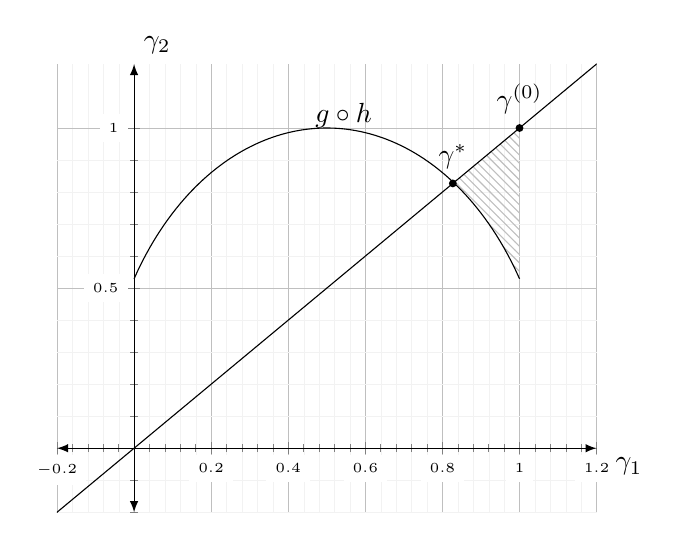
\begin{tikzpicture}
  \begin{axis}[xmin=0,xmax=1,
              ymin=0,ymax=1,
              grid=both,
              grid style={line width=.1pt, draw=gray!10},
              major grid style={line width=.2pt,draw=gray!50},
              axis lines=middle,
              minor tick num=4,
              enlargelimits={abs=0.2},
              axis line style={latex-latex},
              ticklabel style={font=\tiny, fill=white},
              xlabel style={at={(ticklabel* cs:1)},anchor=north west},
              ylabel style={at={(ticklabel* cs:1)},anchor=south west},
              xlabel = {$~\gamma_1$},
              ylabel = {$\gamma_2$}]
  \addplot[name path=F,black!,domain={0:1}, samples=101] {sqrt(1 - 0.02*(12*x - 6)^2)} node[pos=0.6, above left]{$g \circ h$};
  %Sqrt[1 - 0.0000135558 (-200 + 220 x)^2] mathematica approximate result
  \addplot[name path=G,black,domain={-1:2}] {x};
  \addplot[pattern=north west lines, pattern color=gray!50]fill between[of=F and G, soft clip={domain=0.82:1}];
  \node[label={90:{$\gamma^{(0)}$}},circle,fill,inner sep=1pt] at (axis cs:1,1) {};
  \node[label={90:{$\gamma^*$}},circle,fill,inner sep=1pt] at (axis cs:0.827,0.827) {};
  \end{axis}
  \end{tikzpicture}
  \caption{Area maximisation problem for a scalar case. The objective is to maximise the area between $g \circ h$ and a line, starting from $\gamma^{(0)}$. The result is shown in dashed gray.}
  \label{fig1}
  \end{figure}
  \item In the context of power systems, at the first step ($i = 0$) of the iteration (\ref{iteration}) we solve the minimisation problem (\ref{sysid-nlin}) with linear approximation around $\bm{\gamma}_n = \bm{1}$. This is equivalent to Assumption 2(see previous subsection). At the next iteration the algorithm consequently improves previous estimation converging to the solution. 
\end{itemize}
\end{remark}

Finally, we formalise the resulting identification algorithm with iteration (\ref{iteration}) for a single power line between nodes $n-1$ and $n$  in Algorithm \ref{a1}. 
\begin{algorithm}[ht]
\caption{Local iteration for a single power line.
}
\label{a1}
\begin{algorithmic}[1]
\State $\mathcal{M}_{n-1:n} \coloneqq \{\bm{v}_{k}, |\bm{i}_{k}|, \bm{\theta}_{k} ~\big|~ k=n, n-1 \}$
\Function{LineCalc}{$\mathcal{M}_{n-1:n}, \epsilon, \alpha, \bm{j}_n$}
%\Comment Data, accuracy and step size
\State $i = 0$, $\bm{\gamma}_{n}^{(0)} = \mathbf{1}$
\Do 
\State $\widehat{\bm{z}}_n^{(i)} = \bm{h}(\bm{\gamma}_{n}^{(i)})$
\State $\bm{\gamma}_{n}^{(i+1)} = \bm{\gamma}_{n}^{(i)} - \alpha\Big[\bm{g}(\widehat{\bm{z}}_n^{(i)}) - \bm{\gamma}_{n}^{(i)}\Big]$
%\State $i = i+1$
\doWhile{$\|\bm{g}(\widehat{\bm{z}}_n^{(i)}) - \bm{\gamma}_{n}^{(i)}\|_2 > \epsilon$}
\State \Return $\widehat{z}, \bm{\gamma}$
\EndFunction
\end{algorithmic}
\end{algorithm} 
Note, that this algorithm uses information from the previous line of the network, i.e. it needs $\bm{j}_n$ to be known. Therefore, using the backward model (\ref{l_pi_original}) iteratively we formulate the complete algorithm for a linear feeder identification in Algorithm \ref{a2}
\begin{algorithm}[H]
\caption{BCI algorithm for a linear feeder.}
\label{a2}
\begin{algorithmic}[1]
\State $\mathcal{M} \coloneqq \{\bm{v}_{n}, |\bm{i}_{n}|, \bm{\theta}_{n} ~\big|~ n=1, \ldots, N \} \cup \{ \bm{v}_0 \}$
\Function{BCI}{$\mathcal{M}, \epsilon, \alpha$}
\State $\bm{j}_{N} = \bm{i}_{N}$
\For{$n = N : 1$}
\State $\widehat{\bm{z}}_n, \bm{\gamma}_n = $ \textproc{LineCalc}($\mathcal{M}_{n-1:n}, \epsilon, \alpha, \bm{j}_n$)
\State $\bm{j}_{n-1} = \bm{i}_{n-1} + \bm{j}_{n}\frac{|v_{n}|}{|v_{n-1}|} + \widehat{z}_n^*\frac{|j_{n}|^2}{|v_{n-1}|}$ 
\Comment $(\ast)$ 
\EndFor
\State \Return $\bm{\gamma}, \widehat{\bm{z}}, \bm{j}$
\EndFunction
\end{algorithmic}
\end{algorithm} 
\begin{remark}
Equation $(\ast)$ in the Algorithm \ref{a2} can be obtained from the backward model (\ref{l_pi_original}) after excluding term $e^{i\Delta_n}$. 
\end{remark}


\subsection{Discussion}

The main objective of impedance identification algorithm is to minimise a cost function given by (\ref{cost_function-nlin}) for each power line. In this section we compare the optimality of solutions found by BCI and LBCI algorithms.

Again, consider a power line connecting nodes $n-1$ and $n$. The following proposition holds for solutions found by LBCI and BCI: 
\begin{proposition}
\label{prop_bci_vs_lbci}
Let $(\bm{z}_n^{LBCI}, \bm{1})$ is the solution found by the LBCI algorithm and $(\bm{z}_n^{BCI}, \bm{\gamma}^{BCI}_{n})$ is the solution found by the BCI algorithm.
Also, let $N(\bm{z}_n, \bm{\gamma}_{n}) \coloneqq \big\| \bm{V}_{n-1}\bm{\gamma}_{n} - \bm{v}_{n} - \bm{J}_{n}\bm{Q}_1\bm{z}_{n} \big\|_2^2 + \big\|\bm{V}_{n-1}\sqrt{\bm{1} - \bm{\gamma}^2_{n}} - \bm{J}_{n}\bm{Q}_2\bm{z}_{n} \big\|_2^2$ then
$$N(\bm{z}_n^{BCI}, \bm{\gamma}^{BCI}_{n}) \le N(\bm{z}_n^{LBCI}, \bm{1}),$$
i.e. the BCI algorithm finds the solution that is closer to the optimum of (\ref{pf_network}) than that of LBCI.
\end{proposition}
\begin{proof}
See appendix.
\begin{comment}
Consider a linearised BCI algorithm for the power line between nodes $n-1$ and $n$. The solution it finds satisfies:
\begin{equation*}
\begin{split}
{}& N(\bm{z}_n^{LBCI}, \bm{1}) = \big\| \bm{V}_{n-1} - \bm{v}_{n} - \bm{J}_{n}\bm{Q}_1\bm{z}^{LBCI}_{n} \big\|_2^2 + \\
& + \big\|\bm{J}_{n}\bm{Q}_2\bm{z}^{LBCI}_{n} \big\|_2^2 \ge \big\| \bm{V}_{n-1} - \bm{v}_{n} - \bm{J}_{n}\bm{Q}_1\bm{z}^{LBCI}_{n} \big\|_2^2.
\end{split}
\end{equation*}

The corresponding expressions for $\bm{z}_n^{BCI}$ and $\bm{z}_n^{LBCI}$ are given by:  
\begin{equation*}
\begin{split}
{}& \bm{z}_n^{BCI} = \big[ \bm{J}_{n}\bm{Q}_1 \big]^{\dagger} (\bm{V}_{n-1}\bm{\gamma}^{BCI}_{n} - \bm{v}_{n}), \\
& \bm{z}_n^{LBCI} = \big[ \bm{J}_{n}\bm{Q}_1 \big]^{\dagger} (\bm{V}_{n-1} - \bm{v}_{n}),
\end{split}
\end{equation*}
where $\bm{\gamma}^{BCI}_{n} \le \bm{1}$. Therefore:
\begin{equation*}
\begin{split}
{}& N(\bm{z}_n^{BCI}, \bm{\gamma}^{BCI}_{n}) = \big\| \bm{V}_{n-1}\bm{\gamma}^{BCI}_{n} - \bm{v}_{n} - \bm{J}_{n}\bm{Q}_1\bm{z}^{BCI}_{n} \big\|_2^2 \le\\
& \Big\|\big[ \bm{I} - \bm{J}_{n}\bm{Q}_1\big[ \bm{J}_{n}\bm{Q}_1 \big]^{\dagger}\big](\bm{V}_{n-1}\bm{\gamma}^{BCI}_{n} - \bm{v}_{n})\Big\|_2^2 \le \\
& \Big\|\big[ \bm{I} - \bm{J}_{n}\bm{Q}_1\big[ \bm{J}_{n}\bm{Q}_1 \big]^{\dagger}\big](\bm{V}_{n-1} - \bm{v}_{n})\Big\|_2^2 = \\
& \big\| \bm{V}_{n-1} - \bm{v}_{n} - \bm{J}_{n}\bm{Q}_1\bm{z}^{LBCI}_{n} \big\|_2^2 \le N(\bm{z}_n^{LBCI}, \bm{1}).
\end{split}
\end{equation*}
\end{comment}
\end{proof}
\begin{corollary} \label{corollary} In the presence of high measurement noise, we can introduce a regularisation term (as in the LBCI case) for BCI algorithm so that:
$N(\bm{z}_n^{BCI}, \bm{\gamma}^{BCI}_{n}) \le N(\bm{z}_n^{LBCI}, \bm{1})$. 
\begin{proof}
See appendix.
\end{proof}

\begin{comment}
To see this, note that:
\begin{equation*}
\begin{split}
{}& N(\bm{z}_n^{BCI}, \bm{\gamma}^{BCI}_{n}) \le \Big\|\big[ \bm{I} - \bm{J}_{n}\bm{Q}_1\big[ \bm{J}_{n}\bm{Q}_1 \big]^{\dagger}\big](\bm{V}_{n-1} - \bm{v}_{n})\Big\|_2^2 \le \\
& \Big\|\big[ \bm{I} - \bm{J}_{n}\bm{Q}_1\big[ \bm{J}_{n}\bm{Q}_1 \big]^{\dagger}\big](\bm{V}_{n-1} - \bm{v}_{n})\Big\|_2^2 + \mu \big\|\bm{J}_{n}\bm{Q}_2\bm{z}^{BCI}_{n} \big\|_2^2 \le \\
& \Big\|\big[ \bm{I} - \bm{J}_{n}\bm{Q}_1\big[ \bm{J}_{n}\bm{Q}_1 \big]^{\dagger}\big](\bm{V}_{n-1} - \bm{v}_{n})\Big\|_2^2 + \big\|\bm{J}_{n}\bm{Q}_2\bm{z}^{LBCI}_{n} \big\|_2^2 = \\
& N(\bm{z}_n^{LBCI}, \bm{1}),
\end{split}
\end{equation*}
where $0 \le \mu \le 1$ is a regularisation parameter.
\end{comment}
\end{corollary}
Importantly, all the key properties of the LBCI algorithm are inhereted by the BCI algorithm, since $\bm{h}(\bm{\gamma}_{n}^{(i)})$ is a least squares solution of the unconstrained problem (\ref{sysid-nlin}) for a given $\bm{\gamma}_{n}^{(i)}$. 

\subsection{Practical modifications}
\label{practical_modifications_section}
This subsection describes some additional modifications that improve the LBCI/BCI algorithm performance. 

We start from the idea of decentralised calculations, whereby the BCI algorithm above can be executed by smart meters in a decentralised manner with a modification to take advantage of a known $X/R$ ratio\footnote{$X/R$ ratio is the ratio between inductance and resistance of the cable} from cable data. 

\textbf{Regularisation}. As was mentioned in the section \ref{remark_nonzero_J}, if elements in $\bm{J}_n$ are equal to zero (or close to it) then $\bm{J}_n$ is no longer a full rank. To address this issue we can add regularisation term to the objective function in (\ref{sysid-nlin}), i.e:
$$\Big\| \bm{V}_{n-1}\bm{\gamma}_{n} - \bm{v}_{n} - \bm{J}_{n}\bm{Q}_1\bm{z}_{n} \Big\|_2^2 + \mu\|D\bm{z}_n\|_2^2,$$
where $0 \le \mu \le 1, D = \bm{J}_{n}\bm{Q}_2$ as was discussed in the previous subsection. However, note that the choice of $D$ and $\mu$ depends on a priori knowledge about power lines in the network. Thus an algorithm designer might want to incorporate information, that $X/R$ ratio for a cable is close to 1, by making $D = [1~ -1]$.

\textbf{X/R modification}. One method to improve algorithm performance with respect to noise is to use reactance-to-resistance ratio ($k_n$ for $n$-th power line) usually available from cable specifications. The matrix $\bm{J}_n$ (first defined in (\ref{cost_function-lin})) with $X/R$ modification becomes a vector of size $M$ by $1$, therefore its condition number $\kappa(\bm{J}_n) = 1$, which leads to a better noise resistivity for impedance estimation:
\begin{equation*}
\bm{J}_n = \Real{(\bm{j}_n)} - k_n\Imag{(\bm{j}_n)}.
\end{equation*}
Whenever the algorithm has information about $X/R$ ratio of a cable we add subscript $(\cdot)_{XR}$ to its name, i.e. BCI$_{XR}$ or LBCI$_{XR}$.

\textbf{Decentralisation}. The LBCI/BCI algorithm estimates power line impedances for all nodes by processing them sequentially. Thus, for large scale networks large memory required in order to store information from all smart meters. However, every iteration uses data only from neighbouring nodes, therefore one iteration can be encapsulated within one smart metering device capable of obtaining data from adjacent nodes, i.e. from neighbouring smart meters. This makes the grid estimation procedure secure and scalable.

\begin{figure}[t]
\centering
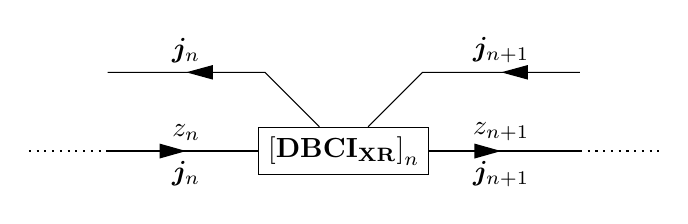
\begin{tikzpicture}
\draw[dotted, thick] (0,0) -- (1,0);
\node at (4,0) [rectangle,draw] (SM_n) {$\mathbf{[DBCI_{XR}]}_{n}$};
\draw[thick] (1,0) -- (SM_n);
\draw[arrows = {-Stealth[inset=0pt, angle=30:10pt]}, thick] (1,0) -- (2, 0)  node[below]{$\bm{j}_{n}$} node[above]{$z_{n}$};
\draw[thick] (SM_n) -- (7,0);
\draw[dotted, thick] (7,0) -- (8,0);
\draw[arrows = {-Stealth[inset=0pt, angle=30:10pt]}, thick] (SM_n) -- (6,0)  node[below]{$\bm{j}_{n+1}$} node[above]{$z_{n+1}$};
%\draw[arrows = {-Stealth[fill=none, inset=0pt, angle=90:10pt]}, thick] (SM_n) -- (4,-1);
\draw (1,1) -- (3,1) -- (SM_n);
\draw[arrows = {-Stealth[inset=0pt, angle=30:10pt]}] (3, 1) -- (2, 1) node[above]{$\bm{j}_{n}$};
\draw (SM_n) -- (5,1) -- (7,1);
\draw[arrows = {-Stealth[inset=0pt, angle=30:10pt]}] (7, 1) -- (6, 1) node[above]{$\bm{j}_{n+1}$};
%\draw (SM_n) -- (5,-1) -- (7,-1) node[above]{output} node[pos = 1/2, below]{$\bm{j}_{n}, z_{n}$};
\end{tikzpicture}
\caption{Smart meter at $n$-th node. Concept of decentralised BCI with known $X/R$ ratio}
\label{SM_n_bci}
\end{figure}

Consider the case of the BCI algorithm and suppose that every smart meter can communicate with its immediate neighbours and the smart meter at node $n+1$ has already calculated values of $\bm{j}_{n+1}$ as in Fig. \ref{SM_n_bci}. Then it sends data to the adjacent smart meter at the $n$-th node, which now has enough information to calculate the impedance of the power line connecting these two meters by performing several iterations of the original BCI algorithm. In addition, it calculates the input current $\mathbf{j}_{n}$ and sends it further up the feeder to the next smart meter and so on. Furthermore, this approach allows each device to have its own information about the $X/R$ ratio for the power lines to which it is connected. The resulting algorithm is called Decentralised BCI with $X/R$ modification, i.e. DBCI$_{XR}$.

\section{Numerical simulations}
\label{num_sim_section}
In order to test the algorithms a single phase power network linear feeder as in Fig. \ref{f1} was implemented in MATLAB/Simulink with $N = 10$. Each power line is modeled as a series connection of resistance and inductance, which is realistic for low voltage overhead lines up to 1-2 km in length \cite{glover2012power}. Loads are modeled as a parallel connection of resistance, inductance and capacitance. Their load shapes are taken from IEEE Low Voltage European Test Feeder data with minute resolution measurements. Although some domestic loads consist of a very complicated composition of resistive, inductive and nonlinear parts \cite{barker2013empirical, pipattanasomporn2014load} we limit our simulations as described above, since our algorithm has full information about load impedances via smart meter measurements (i.e. algorithms do not require load impedances that can be accurately modelled by). We conduct 5000 measurements for all tests, which is equivalent to around 4 days of a network operation.

\subsection{LBCI/BCI testing under ideal conditions}
\begin{figure*}[t]
\begin{subfigure}{0.33\linewidth}
\centering
\begin{adjustbox}{width=1\columnwidth}
% This file was created by matlab2tikz.
%
%The latest updates can be retrieved from
%  http://www.mathworks.com/matlabcentral/fileexchange/22022-matlab2tikz-matlab2tikz
%where you can also make suggestions and rate matlab2tikz.
%
\documentclass[tikz]{standalone}
\usepackage[T1]{fontenc}
\usepackage[utf8]{inputenc}
\usepackage{pgfplots}
\usepackage{grffile}
\pgfplotsset{compat=newest}
\usetikzlibrary{plotmarks}
\usepgfplotslibrary{patchplots}
\usepackage{amsmath}

\begin{document}
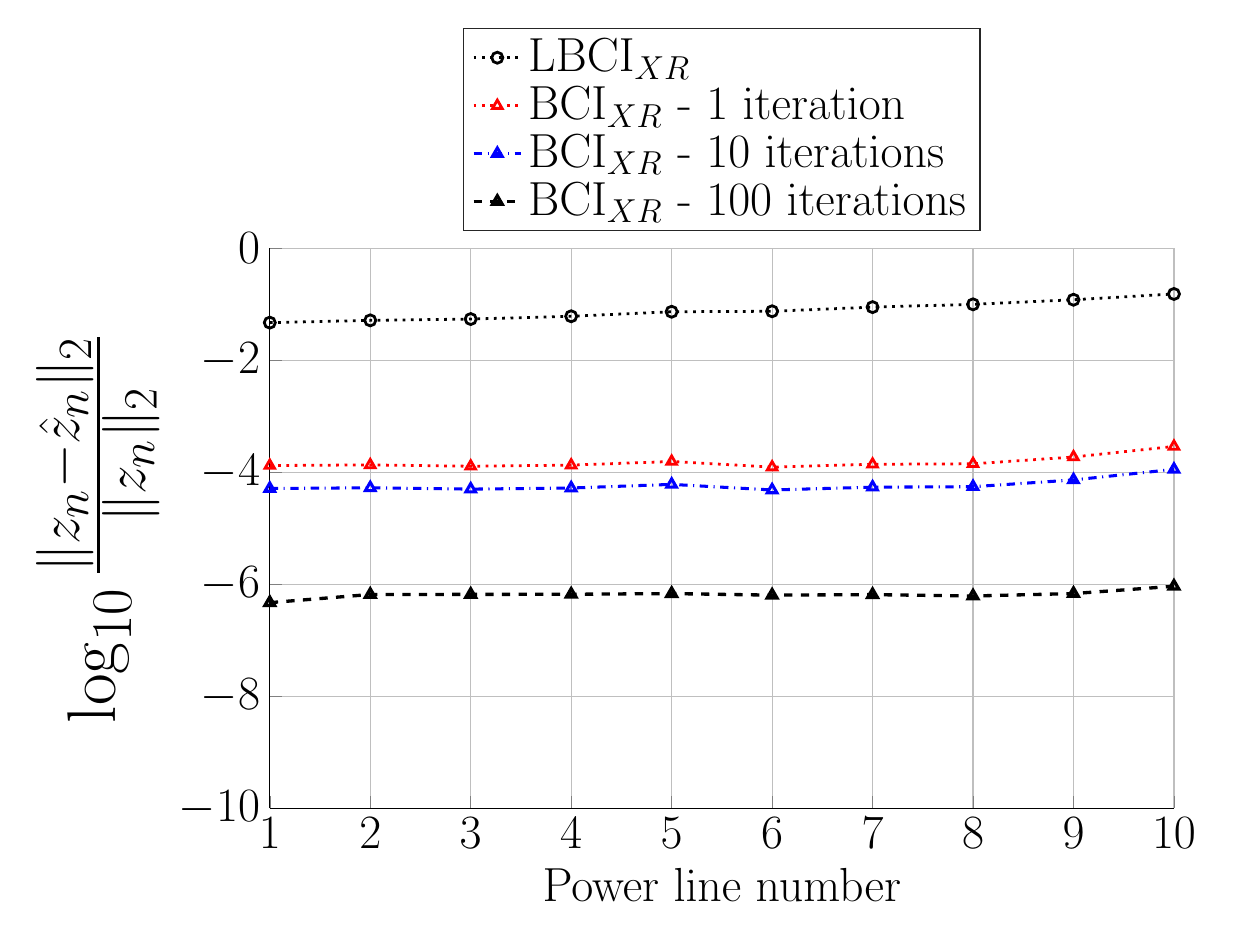
\begin{tikzpicture}

\begin{axis}[%
width=4.521in,
height=2.8in,
at={(0.758in,0.428in)},
scale only axis,
xmin=1,
xmax=10,
xlabel={Power line number},
xmajorgrids,
ymin=-10,
ymax=0,
ylabel={$\log_{10}\frac{\|z_n - \hat{z}_n\|_2}{\|z_n\|_2}$},
ymajorgrids,
axis background/.style={fill=white},
axis x line*=bottom,
axis y line*=left,
legend style={at={(0.5,1.03)},anchor=south,legend cell align=left,align=left,draw=white!15!black},
xlabel style={font=\LARGE},ylabel style={font=\Huge},legend style={font=\LARGE},ticklabel style={font=\LARGE}
]
\addplot [color=black,dotted,line width=1.0pt,mark=o,mark options={solid}]
  table[row sep=crcr]{%
1	-1.32915348006689\\
2	-1.28838246544068\\
3	-1.26512606312045\\
4	-1.21536180362297\\
5	-1.13471057657888\\
6	-1.1261945142969\\
7	-1.0519885476118\\
8	-1.00224806304511\\
9	-0.92036333225634\\
10	-0.817139363952442\\
};
\addlegendentry{LBCI$_{XR}$};

\addplot [color=red,dotted,line width=1.0pt,mark=triangle,mark options={solid}]
  table[row sep=crcr]{%
1	-3.88090534345849\\
2	-3.86964700560886\\
3	-3.89331250305145\\
4	-3.8735781693953\\
5	-3.80841453476826\\
6	-3.9087658497897\\
7	-3.85832000821522\\
8	-3.84983152727818\\
9	-3.7284474352639\\
10	-3.53956216259043\\
};
\addlegendentry{BCI$_{XR}$ - 1 iteration};

\addplot [color=blue,dashdotted,line width=1.1pt,mark=triangle,mark options={solid}]
  table[row sep=crcr]{%
1	-4.2904174938234\\
2	-4.2782761821511\\
3	-4.3017398517945\\
4	-4.28214763461237\\
5	-4.21739012037145\\
6	-4.31717221726016\\
7	-4.26705948823946\\
8	-4.25880740157296\\
9	-4.1379507097733\\
10	-3.94946741399456\\
};
\addlegendentry{BCI$_{XR}$ - 10 iterations};

\addplot [color=black,dashed,line width=1.2pt,mark=triangle,mark options={solid}]
  table[row sep=crcr]{%
1	-6.32939409637337\\
2	-6.1831584219856\\
3	-6.18189088210376\\
4	-6.17946507361347\\
5	-6.16732048573507\\
6	-6.1952229482674\\
7	-6.18612232114627\\
8	-6.21054085497848\\
9	-6.16700097486536\\
10	-6.03675702928428\\
};
\addlegendentry{BCI$_{XR}$ - 100 iterations};

\end{axis}
\end{tikzpicture}%
\end{document}
\end{adjustbox}
\end{subfigure}
\begin{subfigure}{0.33\linewidth}
\centering
\begin{adjustbox}{width=1\columnwidth}
% This file was created by matlab2tikz.
%
%The latest updates can be retrieved from
%  http://www.mathworks.com/matlabcentral/fileexchange/22022-matlab2tikz-matlab2tikz
%where you can also make suggestions and rate matlab2tikz.
%
\documentclass[tikz]{standalone}
\usepackage[T1]{fontenc}
\usepackage[utf8]{inputenc}
\usepackage{pgfplots}
\usepackage{grffile}
\pgfplotsset{compat=newest}
\usetikzlibrary{plotmarks}
\usepgfplotslibrary{patchplots}
\usepackage{amsmath}

\begin{document}
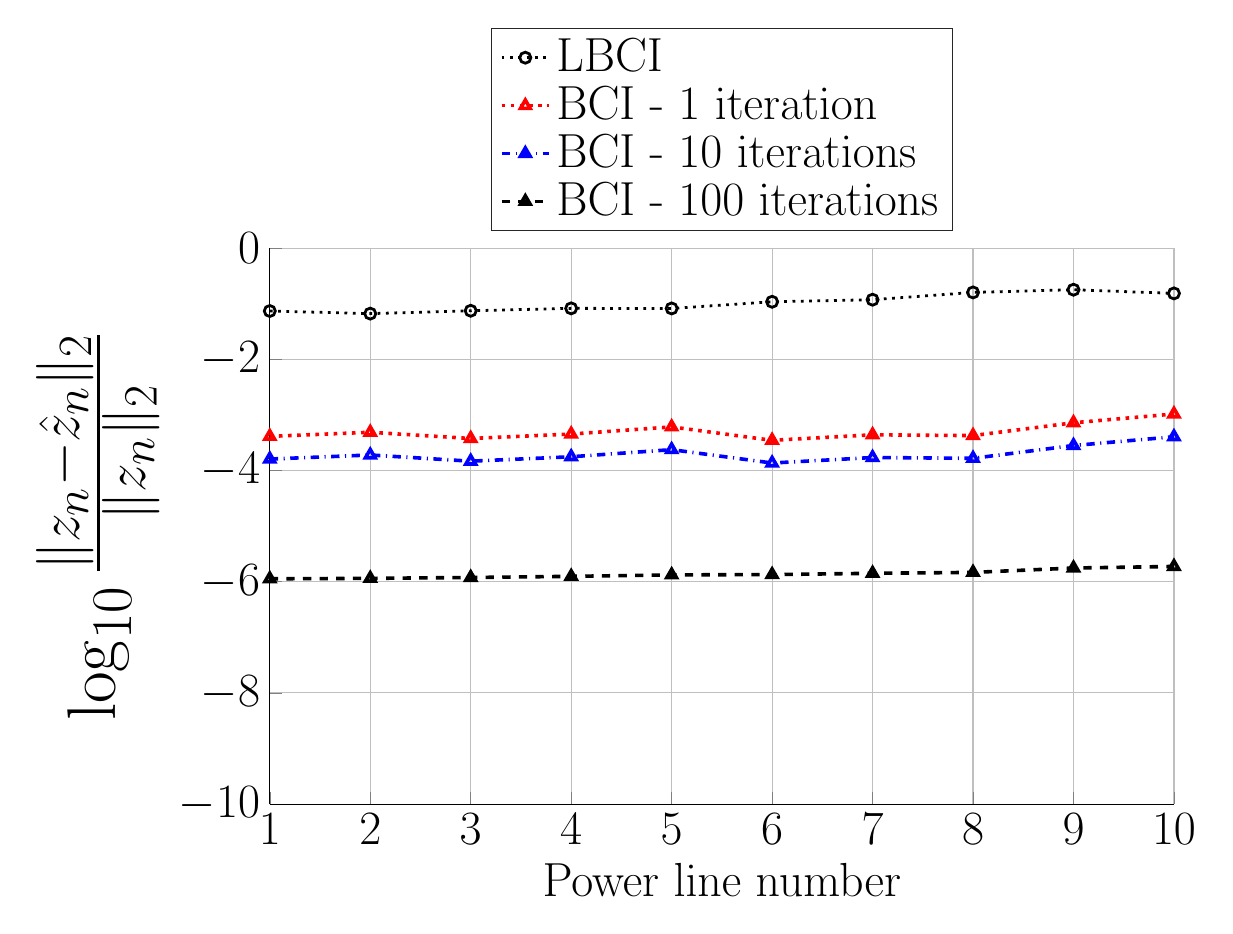
\begin{tikzpicture}

\begin{axis}[%
width=4.521in,
height=2.78in,
at={(0.758in,0.426in)},
scale only axis,
xmin=1,
xmax=10,
xlabel={Power line number},
xmajorgrids,
ymin=-10,
ymax=0,
ylabel={$\log_{10}\frac{\|z_n - \hat{z}_n\|_2}{\|z_n\|_2}$},
ymajorgrids,
axis background/.style={fill=white},
axis x line*=bottom,
axis y line*=left,
legend style={at={(0.5,1.03)},anchor=south,legend cell align=left,align=left,draw=white!15!black},
xlabel style={font=\LARGE},ylabel style={font=\Huge},legend style={font=\LARGE},ticklabel style={font=\LARGE}
]
\addplot [color=black,dotted,line width=1.0pt,mark=o,mark options={solid}]
  table[row sep=crcr]{%
1	-1.13177450249518\\
2	-1.17857232776077\\
3	-1.12729593343788\\
4	-1.08402522530668\\
5	-1.08559823954618\\
6	-0.96567971180553\\
7	-0.92846518739287\\
8	-0.797322672080543\\
9	-0.748880390548875\\
10	-0.814977925085405\\
};
\addlegendentry{LBCI};

\addplot [color=red,dotted,line width=1.3pt,mark=triangle,mark options={solid}]
  table[row sep=crcr]{%
1	-3.38652769511604\\
2	-3.3125017754448\\
3	-3.42454108436879\\
4	-3.34459142874997\\
5	-3.21636110316632\\
6	-3.45741188077818\\
7	-3.35822040183589\\
8	-3.37239749939876\\
9	-3.14154963894484\\
10	-2.98392482454151\\
};
\addlegendentry{BCI - 1 iteration};

\addplot [color=blue,dashdotted,line width=1.3pt,mark=triangle,mark options={solid}]
  table[row sep=crcr]{%
1	-3.79460707876873\\
2	-3.72099482480146\\
3	-3.83273674153348\\
4	-3.7531238584518\\
5	-3.62532359196459\\
6	-3.86566185875066\\
7	-3.76694141604543\\
8	-3.78111340125635\\
9	-3.55086554012878\\
10	-3.39352482393243\\
};
\addlegendentry{BCI - 10 iterations};

\addplot [color=black,dashed,line width=1.3pt,mark=triangle,mark options={solid}]
  table[row sep=crcr]{%
1	-5.94810422550278\\
2	-5.9401901905404\\
3	-5.92476973786823\\
4	-5.90395647396985\\
5	-5.87782690940461\\
6	-5.8722849057396\\
7	-5.84927456959633\\
8	-5.8329346642505\\
9	-5.7542133357923\\
10	-5.72594239175156\\
};
\addlegendentry{BCI - 100 iterations};

\end{axis}
\end{tikzpicture}%
\end{document}
\end{adjustbox}
\end{subfigure}
\begin{subfigure}{0.33\linewidth}
\centering
\begin{adjustbox}{width=1\columnwidth}
% This file was created by matlab2tikz.
%
%The latest updates can be retrieved from
%  http://www.mathworks.com/matlabcentral/fileexchange/22022-matlab2tikz-matlab2tikz
%where you can also make suggestions and rate matlab2tikz.
%
\documentclass[tikz]{standalone}
\usepackage[T1]{fontenc}
\usepackage[utf8]{inputenc}
\usepackage{pgfplots}
\usepackage{grffile}
\pgfplotsset{compat=newest}
\usetikzlibrary{plotmarks}
\usepgfplotslibrary{patchplots}
\usepackage{amsmath}

\begin{document}
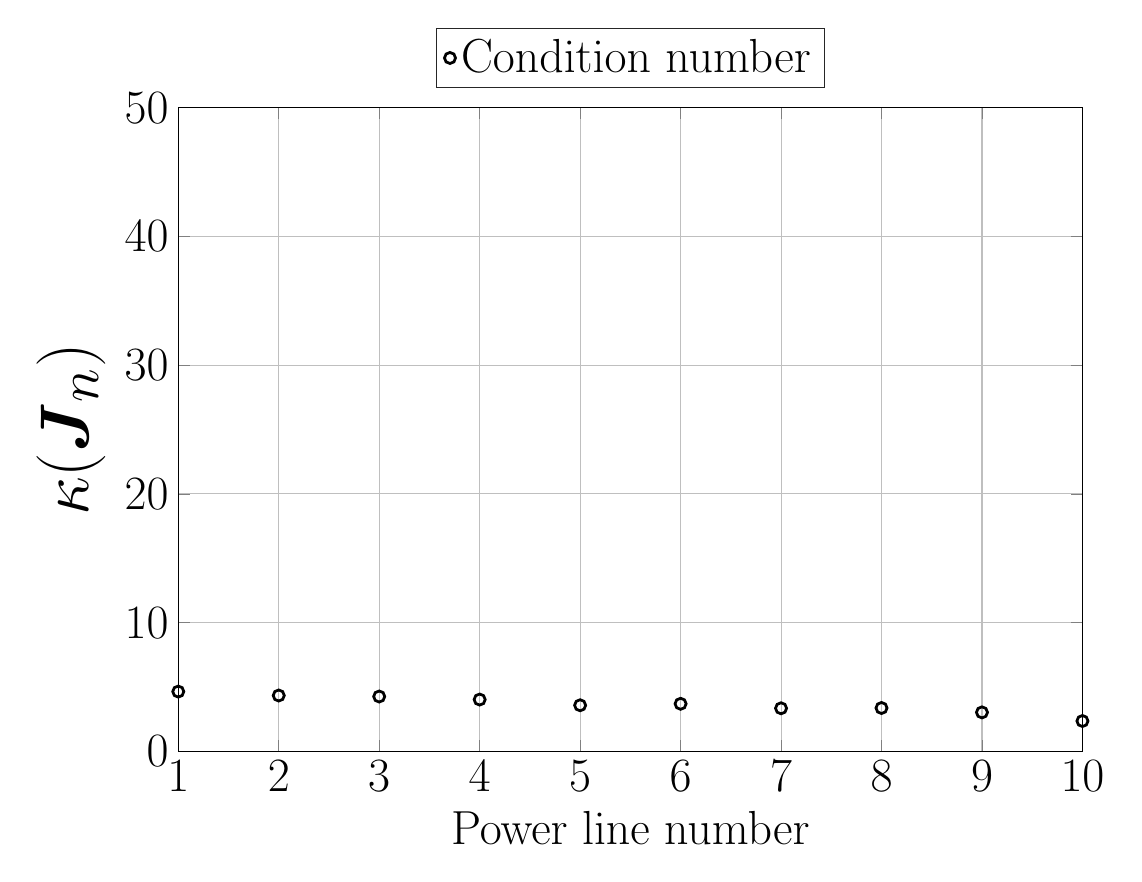
\begin{tikzpicture}

\begin{axis}[%
width=4.521in,
height=3.219in,
at={(0.758in,0.434in)},
scale only axis,
xmin=1,
xmax=10,
xlabel={Power line number},
xmajorgrids,
ymin=0,
ymax=50,
ylabel={$\kappa$(\mbox{\boldmath$J$}$_n$)},
ymajorgrids,
axis background/.style={fill=white},
legend style={at={(0.5,1.03)},anchor=south,legend cell align=left,align=left,draw=white!15!black},
xlabel style={font=\LARGE},ylabel style={font=\Huge},legend style={font=\LARGE},ticklabel style={font=\LARGE}
]
\addplot [color=black,line width=1.0pt,only marks,mark=o,mark options={solid}]
  table[row sep=crcr]{%
1	4.64523681642281\\
2	4.34031112589818\\
3	4.261847277491\\
4	4.02560140250221\\
5	3.58180441458692\\
6	3.69702267447058\\
7	3.34817777291077\\
8	3.36985419389401\\
9	3.02993190395761\\
10	2.35959548143542\\
};
\addlegendentry{Condition number};

\end{axis}
\end{tikzpicture}%
\end{document}
\end{adjustbox}
\end{subfigure}
\caption{Impedance identification error for each power line. FBCI and BCI algorithms under ideal conditions (left, center). Condition number for matrix $\bm{J}_n$(right).}
\label{z_rel_err}
\end{figure*}
We first show BCI performance under ideal conditions, when measuring devices do not have measurement error. To demonstrate the main features of a proposed algorithm we use oversimplified conditions. Each line has the following parameters: length - 50m, $R = 0.4 ~\Omega/km$, $X/R$ ratio - $0.7$. According to IEEE Low Voltage European Test Feeder data description the power factor is kept constant for each load. This is a good assumption for a high level analysis, however, for our algorithms the more detailed behaviour is required. To model uncertainty in power factor we vary it between 0.9 and 1 as a random Gaussian variable ($\mu = 0.95, \sigma = 0.05$) for each load.

We first show algorithm performance with known $X/R$ ratio, since in this case, the result does not depend on the condition number of the measurement matrix ($\bm{J}_n$). Figure \ref{z_rel_err} (left) illustrates identification relative error of BCI algorithm after different number of iterations. The red dotted line on the figure corresponds to the linearised case, i.e. when we assume a small phase difference ($\Delta_n \ll 1$) between two nodes. Blue, and black lines show the relative error after 10 and 100 iterations correspondingly. The step size $\alpha$ was chosen to be 0.1. After about 30 iterations the error is close to simulation accuracy. Note that it is impossible to achieve the same result with LBCI algorithm.

The next figure (Fig. \ref{z_rel_err} - center) compares BCI algorithm performance under ideal conditions with LBCI. Note, that the corresponding line current matrix $\bm{J}_n$ has a condition number around 4-5 for a given set of load shapes from LV European Test Feeder data (Fig. \ref{z_rel_err} - right) and with power factor disturbances introduced. Thus the performance of algorithms is slightly worse than in the previous case, however the result of BCI algorithm is still very close to the simulation accuracy limit.

\begin{figure*}[t]
\begin{subfigure}{0.33\linewidth}
\centering
\begin{adjustbox}{width=1\columnwidth}
% This file was created by matlab2tikz.
%
%The latest updates can be retrieved from
%  http://www.mathworks.com/matlabcentral/fileexchange/22022-matlab2tikz-matlab2tikz
%where you can also make suggestions and rate matlab2tikz.
%
\documentclass[tikz]{standalone}
\usepackage[T1]{fontenc}
\usepackage[utf8]{inputenc}
\usepackage{pgfplots}
\usepackage{grffile}
\pgfplotsset{compat=newest}
\usetikzlibrary{plotmarks}
\usepgfplotslibrary{patchplots}
\usepackage{amsmath}

\begin{document}
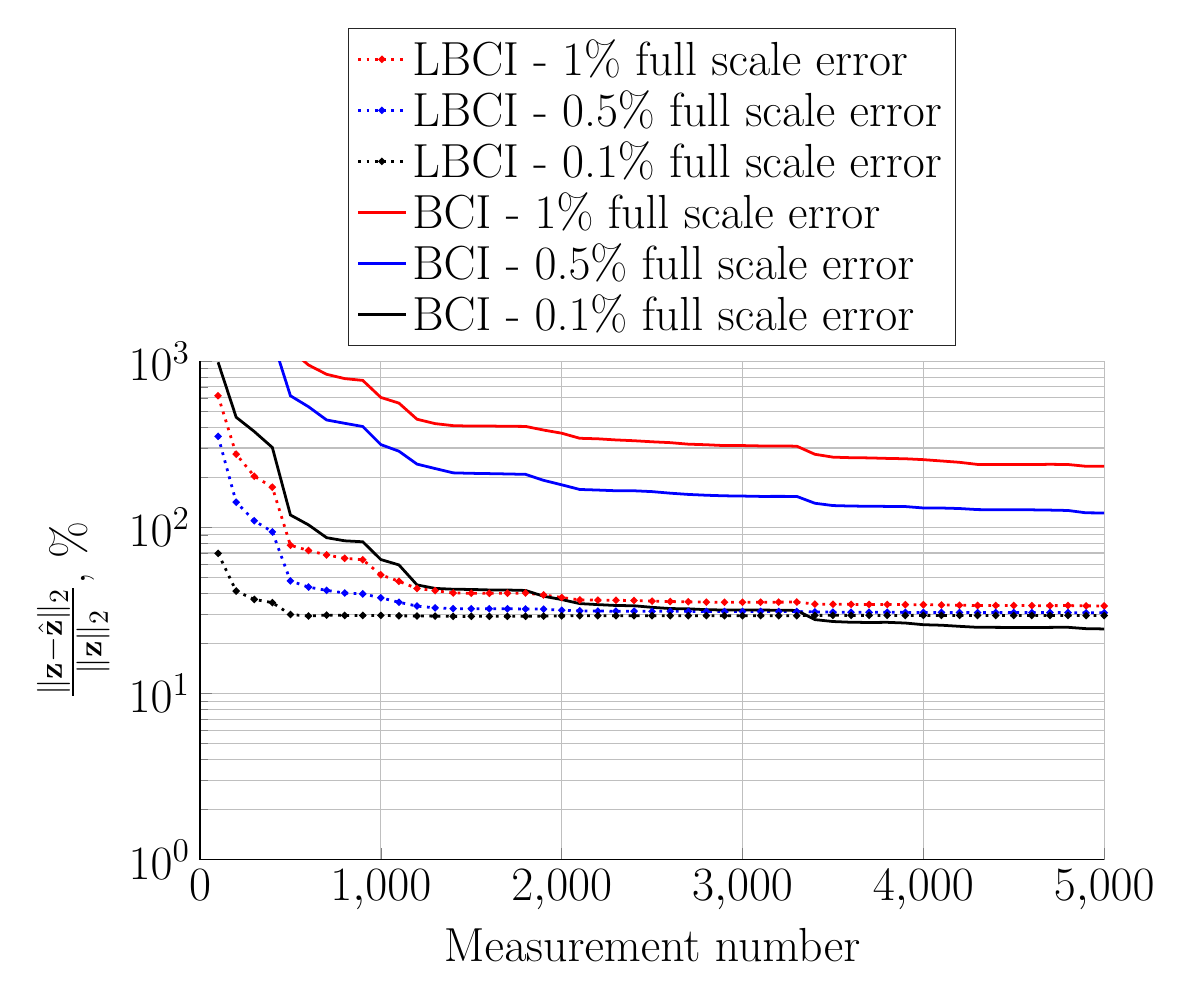
\begin{tikzpicture}

\begin{axis}[%
width=4.521in,
height=2.493in,
at={(0.758in,0.434in)},
scale only axis,
xmin=0,
xmax=5000,
xtick={   0, 1000, 2000, 3000, 4000, 5000},
xlabel={Measurement number},
xmajorgrids,
ymode=log,
ymin=1,
ymax=1000,
yminorticks=true,
ylabel={$\frac{\|\mathbf{z} - \hat{\mathbf{z}}\|_2}{\|\mathbf{z}\|_2}$, \%},
ymajorgrids,
yminorgrids,
axis background/.style={fill=white},
axis x line*=bottom,
axis y line*=left,
legend style={at={(0.5,1.03)},anchor=south,legend cell align=left,align=left,draw=white!15!black},
xlabel style={font=\LARGE},ylabel style={font=\LARGE},legend style={font=\LARGE},ticklabel style={font=\LARGE}
]
\addplot [color=red,dotted,line width=1.0pt,mark size=0.7pt,mark=*,mark options={solid}]
  table[row sep=crcr]{%
100	618.565874809085\\
200	275.107927604509\\
300	202.986394427141\\
400	174.143346467306\\
500	77.93772915443\\
600	72.4416225257139\\
700	68.130107378111\\
800	65.0667628821093\\
900	63.7561722528446\\
1000	51.7593180051441\\
1100	47.3092775501452\\
1200	42.7948503279262\\
1300	41.5649703657043\\
1400	40.206573276376\\
1500	40.1134762264486\\
1600	40.0608865335942\\
1700	40.1136928732485\\
1800	40.173151501695\\
1900	39.1517458543583\\
2000	37.7875296434527\\
2100	36.5566350133897\\
2200	36.4270020595124\\
2300	36.3712161584117\\
2400	36.2440405611231\\
2500	35.9310860897663\\
2600	35.7248430457915\\
2700	35.5989950715627\\
2800	35.4277719465521\\
2900	35.4012206514555\\
3000	35.3804908540011\\
3100	35.3975097979703\\
3200	35.4492057891983\\
3300	35.4581223995724\\
3400	34.5083499897861\\
3500	34.4032826196327\\
3600	34.3648505927901\\
3700	34.3034650004817\\
3800	34.3232839133271\\
3900	34.2287106974776\\
4000	34.181243284833\\
4100	34.0879353992075\\
4200	33.9460640567723\\
4300	33.823089793748\\
4400	33.8199531414247\\
4500	33.7977770801437\\
4600	33.7683935769202\\
4700	33.7532492472821\\
4800	33.8010418043093\\
4900	33.6587794219313\\
5000	33.6306326494405\\
};
\addlegendentry{LBCI - 1\% full scale error};

\addplot [color=blue,dotted,line width=1.0pt,mark size=0.7pt,mark=*,mark options={solid}]
  table[row sep=crcr]{%
100	352.382634256233\\
200	141.486595016329\\
300	109.528793228904\\
400	93.8828649025291\\
500	47.5474668051383\\
600	43.6459362623189\\
700	41.7148773664865\\
800	40.2174833440735\\
900	39.7397686350978\\
1000	37.6573198651872\\
1100	35.3880567887947\\
1200	33.5605349248709\\
1300	32.7347667333502\\
1400	32.3719595766183\\
1500	32.3609412618906\\
1600	32.3367446608151\\
1700	32.3032423781999\\
1800	32.2632910792546\\
1900	32.1606565516506\\
2000	31.6662257856626\\
2100	31.4059364576298\\
2200	31.3181308351929\\
2300	31.2621034199713\\
2400	31.2897254020552\\
2500	31.2111344695258\\
2600	31.2222036000879\\
2700	31.1827690000903\\
2800	31.1497071445986\\
2900	31.1359988180254\\
3000	31.1321275844053\\
3100	31.141145544122\\
3200	31.1473150797466\\
3300	31.1185537155983\\
3400	30.9393761140801\\
3500	30.8373209837428\\
3600	30.8211447532472\\
3700	30.7965717335581\\
3800	30.7844949112658\\
3900	30.7505007424251\\
4000	30.7411402576624\\
4100	30.7399469762595\\
4200	30.7265848120366\\
4300	30.6692474690435\\
4400	30.6695555195663\\
4500	30.6658082373681\\
4600	30.6653088449481\\
4700	30.6646150175997\\
4800	30.6580565496481\\
4900	30.5782424698311\\
5000	30.5738902999195\\
};
\addlegendentry{LBCI - 0.5\% full scale error};

\addplot [color=black,dotted,line width=1.0pt,mark size=0.7pt,mark=*,mark options={solid}]
  table[row sep=crcr]{%
100	69.6455909615255\\
200	41.3148846012258\\
300	36.8130380065506\\
400	35.2075785676292\\
500	29.8549616548759\\
600	29.244258437695\\
700	29.6032842895404\\
800	29.4773332571922\\
900	29.4976766733221\\
1000	29.4920714755628\\
1100	29.3214686254113\\
1200	29.2570577496857\\
1300	29.1827965922184\\
1400	29.0815350040724\\
1500	29.1063535464245\\
1600	29.1084431680269\\
1700	29.1097548731771\\
1800	29.1073153388602\\
1900	29.1909177452964\\
2000	29.2874136347419\\
2100	29.3544777363983\\
2200	29.3607030663155\\
2300	29.3391808035276\\
2400	29.3621378841458\\
2500	29.3505453721207\\
2600	29.3792440764553\\
2700	29.3841195666729\\
2800	29.3752047242743\\
2900	29.3772157040799\\
3000	29.3786861938124\\
3100	29.3784519248367\\
3200	29.3800834837762\\
3300	29.3744658217687\\
3400	29.5027487784969\\
3500	29.5085088000744\\
3600	29.4990539170773\\
3700	29.5035727521978\\
3800	29.4999150721819\\
3900	29.4943933743683\\
4000	29.5041986213115\\
4100	29.4956716273405\\
4200	29.4984608897722\\
4300	29.460671820908\\
4400	29.4614602370312\\
4500	29.460461105279\\
4600	29.4595629204515\\
4700	29.4589453970515\\
4800	29.4563173683792\\
4900	29.4183972736971\\
5000	29.418409849176\\
};
\addlegendentry{LBCI - 0.1\% full scale error};

\addplot [color=red,solid,line width=1.0pt]
  table[row sep=crcr]{%
100	10939.4282794858\\
200	4218.79293382921\\
300	3281.33474638765\\
400	2599.76617799588\\
500	1170.89270892909\\
600	946.600522161743\\
700	832.457314486713\\
800	784.261008542446\\
900	764.901751111227\\
1000	604.08558306595\\
1100	558.460378328972\\
1200	446.674763923221\\
1300	420.315666155738\\
1400	408.609916813595\\
1500	406.24694564777\\
1600	406.574718286192\\
1700	404.942586687761\\
1800	404.423220903262\\
1900	384.465064708311\\
2000	368.070237505923\\
2100	343.030592031864\\
2200	340.612338475662\\
2300	335.327360270985\\
2400	331.652956219918\\
2500	326.826969927445\\
2600	322.933240020542\\
2700	316.194945360981\\
2800	313.676427429031\\
2900	310.011180861667\\
3000	310.141336859814\\
3100	308.570295534127\\
3200	308.716064436462\\
3300	307.42875518688\\
3400	274.8955869407\\
3500	264.132671945233\\
3600	262.119603904118\\
3700	261.396169546429\\
3800	259.571925345053\\
3900	258.32997816703\\
4000	255.150373500367\\
4100	250.501676227442\\
4200	245.907508667846\\
4300	238.767654757424\\
4400	238.504241236432\\
4500	238.65073691125\\
4600	238.449172471361\\
4700	239.149365510132\\
4800	238.593003038806\\
4900	232.695534502624\\
5000	232.857524441911\\
};
\addlegendentry{BCI - 1\% full scale error};

\addplot [color=blue,solid,line width=1.0pt]
  table[row sep=crcr]{%
100	4988.13502781159\\
200	2444.87548208943\\
300	1733.3249857583\\
400	1362.27101754373\\
500	618.336586986953\\
600	531.146403811036\\
700	442.1948107434\\
800	422.191221463147\\
900	403.771786737491\\
1000	314.391176663283\\
1100	286.839637612527\\
1200	239.871235609107\\
1300	225.589302036281\\
1400	212.501253742105\\
1500	211.119466862647\\
1600	210.266081627266\\
1700	209.283377716353\\
1800	208.10170705769\\
1900	191.574028473684\\
2000	180.074443135741\\
2100	168.811777599424\\
2200	167.450518993585\\
2300	165.847538490874\\
2400	165.78422627458\\
2500	163.866224667952\\
2600	160.363277531053\\
2700	157.615577690254\\
2800	155.845124205837\\
2900	154.575970904311\\
3000	154.076091355224\\
3100	153.344013534164\\
3200	153.422976528203\\
3300	153.323579773637\\
3400	139.473256237771\\
3500	135.071348446532\\
3600	134.157554469797\\
3700	133.805378471932\\
3800	133.503207284249\\
3900	133.233338480496\\
4000	130.617395736445\\
4100	130.55064061357\\
4200	129.629425163305\\
4300	127.704815594137\\
4400	127.436836417746\\
4500	127.340412103804\\
4600	127.296991658512\\
4700	126.844783224533\\
4800	126.183289403131\\
4900	122.112369308204\\
5000	121.948639664765\\
};
\addlegendentry{BCI - 0.5\% full scale error};

\addplot [color=black,solid,line width=1.0pt]
  table[row sep=crcr]{%
100	983.097984365482\\
200	459.231063318821\\
300	376.804443565766\\
400	302.00130790956\\
500	118.555779963691\\
600	103.3726771843\\
700	86.5674726763889\\
800	82.8863800904153\\
900	81.7801433011419\\
1000	63.9209324169423\\
1100	59.3539145125219\\
1200	44.9947925703019\\
1300	42.8654739846427\\
1400	42.3791929465445\\
1500	42.2467192621202\\
1600	41.9679996512012\\
1700	41.9195047726181\\
1800	41.6675180370154\\
1900	38.4540225521658\\
2000	36.7329981605019\\
2100	34.7268959936169\\
2200	34.2448428725205\\
2300	33.8342804788993\\
2400	33.7059753690994\\
2500	32.9789583380315\\
2600	32.4221252657376\\
2700	32.3104756296501\\
2800	31.9133046882613\\
2900	31.7772443881123\\
3000	31.7701208348717\\
3100	31.7616112489574\\
3200	31.6857654558978\\
3300	31.5960338000104\\
3400	27.8164634410411\\
3500	27.0915026283469\\
3600	26.8150551735293\\
3700	26.7427908700357\\
3800	26.7904096262388\\
3900	26.5361393411003\\
4000	25.9229387582616\\
4100	25.7398585711523\\
4200	25.3460023141886\\
4300	24.9996313706155\\
4400	24.9843284663807\\
4500	24.9646864664521\\
4600	24.9482414111492\\
4700	24.9808542291075\\
4800	25.0062385390108\\
4900	24.5412230366541\\
5000	24.4458111154257\\
};
\addlegendentry{BCI - 0.1\% full scale error};

\end{axis}
\end{tikzpicture}%
\end{document}
\end{adjustbox}
\end{subfigure}
\begin{subfigure}{0.33\linewidth}
\centering
\begin{adjustbox}{width=1\columnwidth}
% This file was created by matlab2tikz.
%
%The latest updates can be retrieved from
%  http://www.mathworks.com/matlabcentral/fileexchange/22022-matlab2tikz-matlab2tikz
%where you can also make suggestions and rate matlab2tikz.
%
\documentclass[tikz]{standalone}
\usepackage[T1]{fontenc}
\usepackage[utf8]{inputenc}
\usepackage{pgfplots}
\usepackage{grffile}
\pgfplotsset{compat=newest}
\usetikzlibrary{plotmarks}
\usepgfplotslibrary{patchplots}
\usepackage{amsmath}

\begin{document}
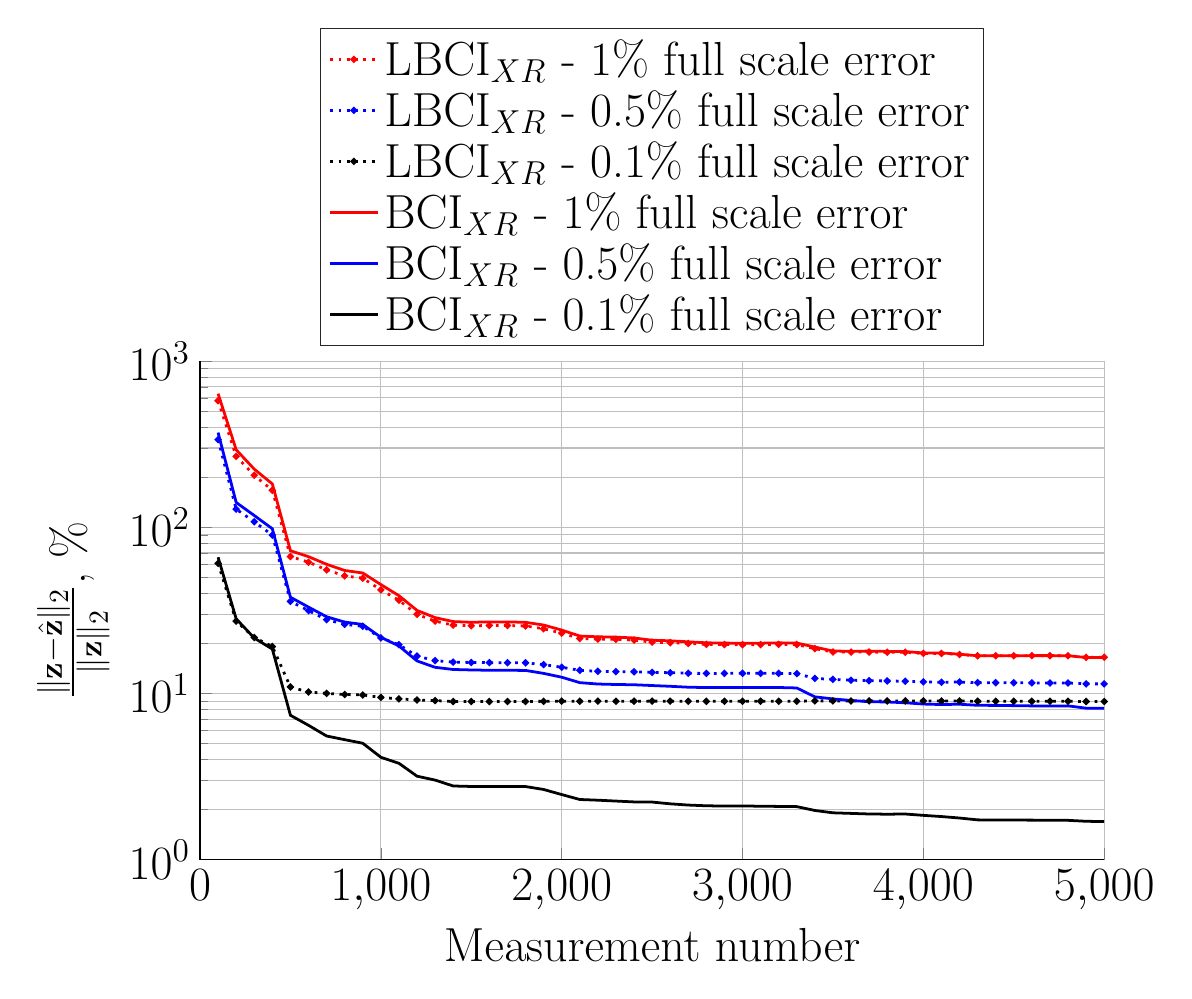
\begin{tikzpicture}

\begin{axis}[%
width=4.521in,
height=2.493in,
at={(0.758in,0.434in)},
scale only axis,
xmin=0,
xmax=5000,
xtick={   0, 1000, 2000, 3000, 4000, 5000},
xlabel={Measurement number},
xmajorgrids,
ymode=log,
ymin=1,
ymax=1000,
yminorticks=true,
ylabel={$\frac{\|\mathbf{z} - \hat{\mathbf{z}}\|_2}{\|\mathbf{z}\|_2}$, \%},
ymajorgrids,
yminorgrids,
axis background/.style={fill=white},
axis x line*=bottom,
axis y line*=left,
legend style={at={(0.5,1.03)},anchor=south,legend cell align=left,align=left,draw=white!15!black},
xlabel style={font=\LARGE},ylabel style={font=\LARGE},legend style={font=\LARGE},ticklabel style={font=\LARGE}
]
\addplot [color=red,dotted,line width=1.0pt,mark size=0.7pt,mark=*,mark options={solid}]
  table[row sep=crcr]{%
100	577.391750400882\\
200	267.093230969695\\
300	205.319242503762\\
400	166.928295300879\\
500	66.644882813857\\
600	61.6679189789651\\
700	55.3852532392064\\
800	50.9604169261538\\
900	49.3675170342762\\
1000	42.0212254866031\\
1100	36.3700843526153\\
1200	29.9193523111009\\
1300	27.2278430482018\\
1400	25.7649706685327\\
1500	25.5327647984282\\
1600	25.6474224322936\\
1700	25.6574706552111\\
1800	25.4680309409088\\
1900	24.5091774128577\\
2000	23.076946555035\\
2100	21.4235929636326\\
2200	21.2421839472294\\
2300	21.1764258356123\\
2400	20.9478765989289\\
2500	20.3576609733448\\
2600	20.2064694206182\\
2700	19.9846228279037\\
2800	19.7587681214098\\
2900	19.6852826688951\\
3000	19.6657931119346\\
3100	19.6560772678979\\
3200	19.739210201449\\
3300	19.6835829537958\\
3400	18.6071014044608\\
3500	17.7729543095237\\
3600	17.7295345972129\\
3700	17.7539063172693\\
3800	17.6991400368571\\
3900	17.6828713873297\\
4000	17.4070259473985\\
4100	17.4172552304756\\
4200	17.1499873281785\\
4300	16.8575389581397\\
4400	16.868921028951\\
4500	16.8657273675102\\
4600	16.8760096189548\\
4700	16.8776479981479\\
4800	16.8635141639981\\
4900	16.497290253911\\
5000	16.5219252269178\\
};
\addlegendentry{LBCI$_{XR}$ - 1\% full scale error};

\addplot [color=blue,dotted,line width=1.0pt,mark size=0.7pt,mark=*,mark options={solid}]
  table[row sep=crcr]{%
100	336.645848518894\\
200	128.554202881726\\
300	107.91341470573\\
400	89.7008586225277\\
500	35.8305282561023\\
600	31.5147132341474\\
700	27.8205188450343\\
800	26.0399639208426\\
900	25.373910928077\\
1000	21.5908272677598\\
1100	19.665633555213\\
1200	16.7821611898977\\
1300	15.7642012447506\\
1400	15.4424522531692\\
1500	15.3629412812489\\
1600	15.3227855127073\\
1700	15.3042926181891\\
1800	15.2809154453315\\
1900	14.9187553765836\\
2000	14.3766246539883\\
2100	13.7706769744652\\
2200	13.6016477410138\\
2300	13.5306006602\\
2400	13.4899507193898\\
2500	13.3924228474751\\
2600	13.3308271756306\\
2700	13.2275946373813\\
2800	13.1932006033215\\
2900	13.2074808783891\\
3000	13.2153492814913\\
3100	13.2121605727348\\
3200	13.2095297553954\\
3300	13.1620105508672\\
3400	12.3088178147556\\
3500	12.1544657262373\\
3600	12.0160245126537\\
3700	11.9270114174846\\
3800	11.8946433629559\\
3900	11.8375568689779\\
4000	11.7292897638418\\
4100	11.6841083720192\\
4200	11.709783417035\\
4300	11.6190952873433\\
4400	11.6143501006531\\
4500	11.592644405011\\
4600	11.5742624064494\\
4700	11.554518002781\\
4800	11.5694556420955\\
4900	11.423074472196\\
5000	11.4175127490441\\
};
\addlegendentry{LBCI$_{XR}$ - 0.5\% full scale error};

\addplot [color=black,dotted,line width=1.0pt,mark size=0.7pt,mark=*,mark options={solid}]
  table[row sep=crcr]{%
100	60.6232061565378\\
200	27.2289448057352\\
300	21.7268329589992\\
400	19.1635426659609\\
500	10.9431204082108\\
600	10.1947024844337\\
700	10.0140096348267\\
800	9.85809285195655\\
900	9.80178458581397\\
1000	9.46487266176593\\
1100	9.28310922112982\\
1200	9.13196395568197\\
1300	9.06044621194058\\
1400	8.93904581145372\\
1500	8.94388026207321\\
1600	8.94197512933743\\
1700	8.94582080975783\\
1800	8.94689282566839\\
1900	8.96661443409027\\
2000	8.99318668403021\\
2100	8.97789317908973\\
2200	8.98827643088499\\
2300	8.9771309821604\\
2400	8.98788038408225\\
2500	8.99255464487493\\
2600	8.98933336210284\\
2700	8.98233202696932\\
2800	8.97437072482077\\
2900	8.98022976246306\\
3000	8.98257483406135\\
3100	8.97941213292436\\
3200	8.97433050709443\\
3300	8.96974470624438\\
3400	9.02449448128123\\
3500	9.02438520888396\\
3600	9.01713476981925\\
3700	9.0206951925146\\
3800	9.01921761024206\\
3900	9.01760644990102\\
4000	9.01844924824081\\
4100	9.00894158839334\\
4200	9.00713181772295\\
4300	8.97885211895225\\
4400	8.97795544281009\\
4500	8.97601619209\\
4600	8.97468330161962\\
4700	8.97311973683783\\
4800	8.97175386011031\\
4900	8.94679929163184\\
5000	8.94983106818811\\
};
\addlegendentry{LBCI$_{XR}$ - 0.1\% full scale error};

\addplot [color=red,solid,line width=1.0pt]
  table[row sep=crcr]{%
100	636.500144257714\\
200	292.676529266655\\
300	223.795513847441\\
400	182.346181281471\\
500	72.2391461623452\\
600	66.5647500460818\\
700	59.8727928669973\\
800	54.9590912238281\\
900	53.0709276860564\\
1000	45.2094835288144\\
1100	38.7612198601652\\
1200	31.6039078982571\\
1300	28.6101670171299\\
1400	27.0686490062978\\
1500	26.8127530888437\\
1600	26.9539956248889\\
1700	26.952166385095\\
1800	26.7900874503672\\
1900	25.8048499970827\\
2000	24.0780007369917\\
2100	22.1563269154779\\
2200	21.9291605690581\\
2300	21.82142918688\\
2400	21.5762728588356\\
2500	20.9036726252275\\
2600	20.7442032531047\\
2700	20.450458762919\\
2800	20.1757940868614\\
2900	20.0890369152345\\
3000	20.0641691491575\\
3100	20.0629870030643\\
3200	20.1631784593289\\
3300	20.1094427897021\\
3400	19.0207477509391\\
3500	18.0006920405027\\
3600	17.9482466160831\\
3700	17.9855167035162\\
3800	17.9127744576634\\
3900	17.8743480688399\\
4000	17.5283624638278\\
4100	17.543397666076\\
4200	17.2208643332019\\
4300	16.8681730969016\\
4400	16.8778226724616\\
4500	16.87658311737\\
4600	16.8880211110168\\
4700	16.8939169017106\\
4800	16.8741869033947\\
4900	16.4524265610638\\
5000	16.4710227186601\\
};
\addlegendentry{BCI$_{XR}$ - 1\% full scale error};

\addplot [color=blue,solid,line width=1.0pt]
  table[row sep=crcr]{%
100	371.34684258334\\
200	141.004301187621\\
300	117.709262864169\\
400	97.9572088257102\\
500	37.9426917051369\\
600	33.0808380413626\\
700	28.9504901330387\\
800	26.8795429042067\\
900	26.0117379109377\\
1000	21.7736645458502\\
1100	19.3172803174777\\
1200	15.6951061027285\\
1300	14.364146130252\\
1400	13.9415796632522\\
1500	13.8479745269059\\
1600	13.791722702049\\
1700	13.7857650049981\\
1800	13.7599606682894\\
1900	13.2075572092958\\
2000	12.5249694456453\\
2100	11.6182954572368\\
2200	11.395892596789\\
2300	11.3223075802414\\
2400	11.2836252705669\\
2500	11.1598111517771\\
2600	11.0436340217559\\
2700	10.9057020441624\\
2800	10.8514999045513\\
2900	10.8446097573783\\
3000	10.8596901588358\\
3100	10.8484737656465\\
3200	10.861178873008\\
3300	10.7914180988687\\
3400	9.54348935647062\\
3500	9.27100120291306\\
3600	9.07527673743194\\
3700	8.91996663317877\\
3800	8.88739559824935\\
3900	8.78998380310235\\
4000	8.63453034733242\\
4100	8.57720408146672\\
4200	8.61412132044649\\
4300	8.48513726562341\\
4400	8.47561462705886\\
4500	8.44670705081155\\
4600	8.41733050783347\\
4700	8.39226701405558\\
4800	8.42067572309058\\
4900	8.15614971251391\\
5000	8.13779609290959\\
};
\addlegendentry{BCI$_{XR}$ - 0.5\% full scale error};

\addplot [color=black,solid,line width=1.0pt]
  table[row sep=crcr]{%
100	66.0141848328862\\
200	28.1320284190169\\
300	21.5494579753043\\
400	18.4927117515729\\
500	7.3930446912482\\
600	6.43355363669567\\
700	5.54636554178825\\
800	5.27268540100493\\
900	5.01692690104795\\
1000	4.13232294071725\\
1100	3.80109360438199\\
1200	3.17910427037647\\
1300	3.01203361217865\\
1400	2.77510632773033\\
1500	2.75677356937227\\
1600	2.7531736562209\\
1700	2.75223068924941\\
1800	2.75386088602477\\
1900	2.64407600640884\\
2000	2.46433665573116\\
2100	2.30158312768054\\
2200	2.27918385424576\\
2300	2.25211115169549\\
2400	2.22548639306507\\
2500	2.221428322728\\
2600	2.1676407010861\\
2700	2.13066887267363\\
2800	2.10949762752772\\
2900	2.10159633004459\\
3000	2.10565987103901\\
3100	2.0959100868024\\
3200	2.09131624004766\\
3300	2.08504415791899\\
3400	1.97707125929211\\
3500	1.91400306597603\\
3600	1.89868012631728\\
3700	1.88293101620837\\
3800	1.87764129602836\\
3900	1.88245095796468\\
4000	1.84775182684586\\
4100	1.817556606915\\
4200	1.78064496623178\\
4300	1.73535891599895\\
4400	1.73344057879927\\
4500	1.73023002720965\\
4600	1.72951855580784\\
4700	1.72615288625156\\
4800	1.72459825576531\\
4900	1.70165967800584\\
5000	1.69530490101971\\
};
\addlegendentry{BCI$_{XR}$ - 0.1\% full scale error};

\end{axis}
\end{tikzpicture}%
\end{document}
\end{adjustbox}
\end{subfigure}
\begin{subfigure}{0.33\linewidth}
\centering
\begin{adjustbox}{width=1\columnwidth}
% This file was created by matlab2tikz.
%
%The latest updates can be retrieved from
%  http://www.mathworks.com/matlabcentral/fileexchange/22022-matlab2tikz-matlab2tikz
%where you can also make suggestions and rate matlab2tikz.
%
\documentclass[tikz]{standalone}
\usepackage[T1]{fontenc}
\usepackage[utf8]{inputenc}
\usepackage{pgfplots}
\usepackage{grffile}
\pgfplotsset{compat=newest}
\usetikzlibrary{plotmarks}
\usepgfplotslibrary{patchplots}
\usepackage{amsmath}

\begin{document}
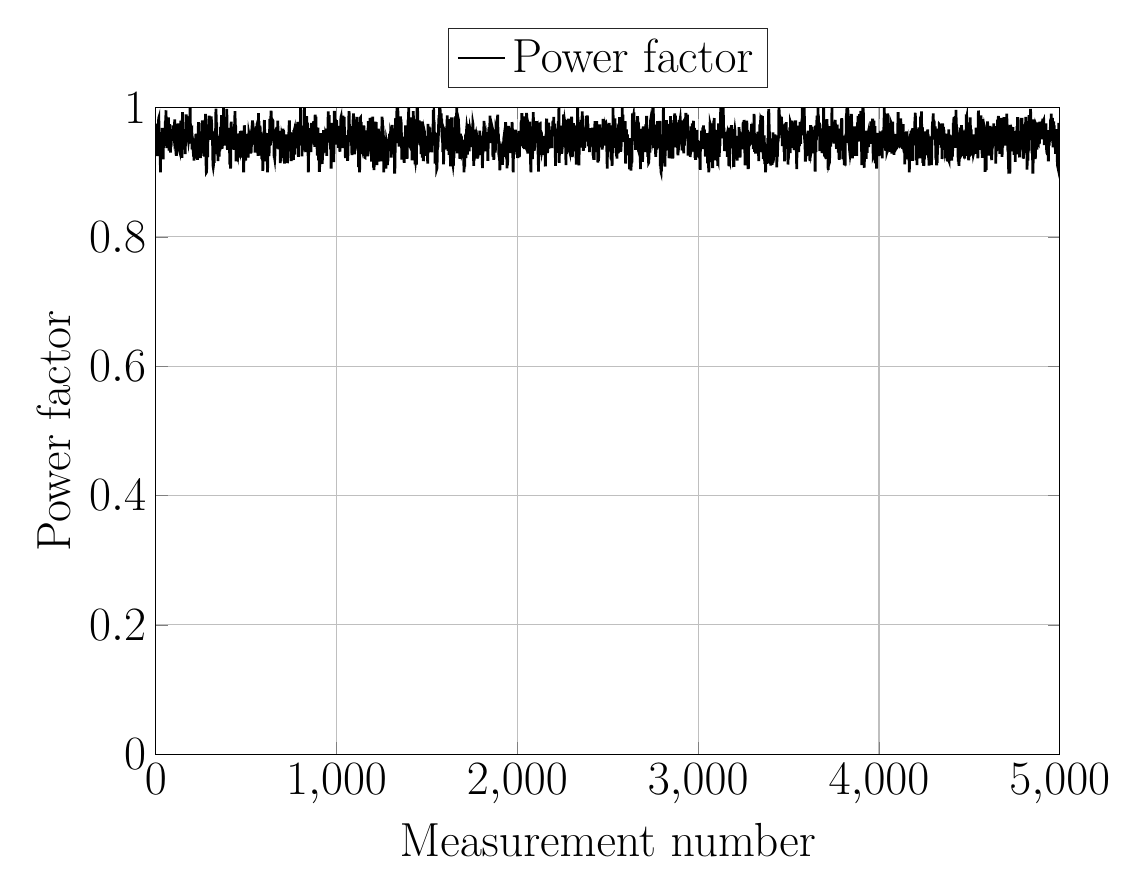
\begin{tikzpicture}

\begin{axis}[%
width=4.52in,
height=3.232in,
at={(0.758in,0.436in)},
scale only axis,
xmin=0,
xmax=5000,
xtick={   0, 1000, 2000, 3000, 4000, 5000},
xlabel={Measurement number},
xmajorgrids,
ymin=0,
ymax=1,
ylabel={Power factor},
ymajorgrids,
axis background/.style={fill=white},
legend style={at={(0.5,1.03)},anchor=south,legend cell align=left,align=left,draw=white!15!black},
xlabel style={font=\LARGE},ylabel style={font=\LARGE},legend style={font=\LARGE},ticklabel style={font=\LARGE}
]
\addplot [color=black,solid,line width=1.0pt,forget plot]
  table[row sep=crcr]{%
1	0.94642384302422\\
2	0.975336575994959\\
3	0.951113973485854\\
4	0.947862268860169\\
5	0.936338926661691\\
6	0.941392756468832\\
7	0.938204076615226\\
8	0.925260306840745\\
9	0.930704969497183\\
10	0.943047800404891\\
11	0.940022432244783\\
12	0.948106239129861\\
13	0.970147335961478\\
14	0.96982257391773\\
15	0.955945790568449\\
16	0.983526592023571\\
17	0.984449516981176\\
18	0.96199584671956\\
19	0.947891554999676\\
20	0.959596952539734\\
21	0.953511341961749\\
22	0.934541709460444\\
23	0.94489673194331\\
24	0.943169775539891\\
25	0.928348666918004\\
26	0.9\\
27	0.940435993053016\\
28	0.957224302800614\\
29	0.946216624815353\\
30	0.955753815787786\\
31	0.944182753360872\\
32	0.943853772948015\\
33	0.934427955770569\\
34	0.95752245721545\\
35	0.959453747757117\\
36	0.968711553076628\\
37	0.96578141228924\\
38	0.945426473662656\\
39	0.934836850733102\\
40	0.936725078742042\\
41	0.919967261991439\\
42	0.934972518621256\\
43	0.960472186860523\\
44	0.946410129475856\\
45	0.954778827375918\\
46	0.940772652678596\\
47	0.958398597045348\\
48	0.954557099828029\\
49	0.963773865429422\\
50	0.951506022926726\\
51	0.954727569201236\\
52	0.9646734785798\\
53	0.977811292974159\\
54	0.979045577451492\\
55	0.975932826416532\\
56	0.987896065848176\\
57	0.995939494185129\\
58	0.966458221918116\\
59	0.967428166249755\\
60	0.945756467097624\\
61	0.937567320201842\\
62	0.954114017154011\\
63	0.949801556414701\\
64	0.961913868974876\\
65	0.937376027279935\\
66	0.959583872365729\\
67	0.94756241685385\\
68	0.942064460863642\\
69	0.963303737801128\\
70	0.984772967751947\\
71	0.972054598128733\\
72	0.959823561350124\\
73	0.964961722314041\\
74	0.933645091134188\\
75	0.956910120434687\\
76	0.956752187225122\\
77	0.974584995686175\\
78	0.967908899028481\\
79	0.973077851628163\\
80	0.952922447931796\\
81	0.930468833736354\\
82	0.956283784600467\\
83	0.957941919893558\\
84	0.939110187783749\\
85	0.949935902073805\\
86	0.941707240433414\\
87	0.966589645266208\\
88	0.955407954414003\\
89	0.9645371615266\\
90	0.960558859329979\\
91	0.949465374949962\\
92	0.953920752299818\\
93	0.954636095104379\\
94	0.958402847204293\\
95	0.965563465125481\\
96	0.961947827049353\\
97	0.97251664582096\\
98	0.958730520423417\\
99	0.959574720908039\\
100	0.959103237980429\\
101	0.956006579302019\\
102	0.958484545240241\\
103	0.966350010682776\\
104	0.975231075971799\\
105	0.981633506406907\\
106	0.974519716785457\\
107	0.971983803674631\\
108	0.956708024415146\\
109	0.962373580831132\\
110	0.936074343001477\\
111	0.935543470551782\\
112	0.927951962233611\\
113	0.930228570359404\\
114	0.92554754703502\\
115	0.946384059459908\\
116	0.958477955130213\\
117	0.960862918234609\\
118	0.955960191348604\\
119	0.946614660633567\\
120	0.950143364843558\\
121	0.953102282595965\\
122	0.964580637460818\\
123	0.974849075582093\\
124	0.959226130077656\\
125	0.962892616470785\\
126	0.975615708294712\\
127	0.951550320815049\\
128	0.961049511530677\\
129	0.965432513583398\\
130	0.970773417793468\\
131	0.93360442531582\\
132	0.932584141855113\\
133	0.957466855471516\\
134	0.94656274795646\\
135	0.956531709784011\\
136	0.952229358326609\\
137	0.959306705370602\\
138	0.967517344472084\\
139	0.980049428305163\\
140	0.970768087185022\\
141	0.967037976400974\\
142	0.942656235815276\\
143	0.923403955261669\\
144	0.939181234796637\\
145	0.922405354616681\\
146	0.943495281304588\\
147	0.979050387349898\\
148	0.992934075207153\\
149	0.988320716274008\\
150	0.964851067393304\\
151	0.952313846948977\\
152	0.961644435785242\\
153	0.952224996583385\\
154	0.960103863349994\\
155	0.951828922188673\\
156	0.948209197735291\\
157	0.940776108235158\\
158	0.939035780780435\\
159	0.938417340258261\\
160	0.941717171915555\\
161	0.937249128113143\\
162	0.942145346829674\\
163	0.928197230865662\\
164	0.943651504354035\\
165	0.954341572389772\\
166	0.961995491388461\\
167	0.969029426190762\\
168	0.97712333724144\\
169	0.989540547584851\\
170	0.979943916991512\\
171	0.98708440521443\\
172	0.967605105399309\\
173	0.962915406718558\\
174	0.957402073053464\\
175	0.956254542786457\\
176	0.958528406749196\\
177	0.963118505730737\\
178	0.98579441793805\\
179	0.94914193052317\\
180	0.950679786271787\\
181	0.948438033611645\\
182	0.95088196921266\\
183	0.962534711844875\\
184	0.983687142083246\\
185	0.979379330419821\\
186	0.983793881977745\\
187	0.96957988368491\\
188	0.973714019217704\\
189	0.990306044994312\\
190	1\\
191	0.984963407992938\\
192	0.96275169259446\\
193	0.944364958086035\\
194	0.952372247055699\\
195	0.960916173890581\\
196	0.959553745473413\\
197	0.95779599084006\\
198	0.968257210090862\\
199	0.968492757558021\\
200	0.958385928835143\\
201	0.935423749903579\\
202	0.956323909258072\\
203	0.951286413085797\\
204	0.939172470940469\\
205	0.93698428787815\\
206	0.934864033298812\\
207	0.933944843764882\\
208	0.92993284018584\\
209	0.924461293910059\\
210	0.952569567997327\\
211	0.927720489916326\\
212	0.917973964490637\\
213	0.935554459910223\\
214	0.931765342082704\\
215	0.926061508316281\\
216	0.923308437247212\\
217	0.929343627835433\\
218	0.937150604777945\\
219	0.934255872906107\\
220	0.948907381477802\\
221	0.950306377436074\\
222	0.959105955428957\\
223	0.953923655267051\\
224	0.959555060268833\\
225	0.955023944702437\\
226	0.93580809227051\\
227	0.921013025629936\\
228	0.939297705462749\\
229	0.95117067905541\\
230	0.93687327822494\\
231	0.919181715942992\\
232	0.934008491932052\\
233	0.928662468531169\\
234	0.933196901351104\\
235	0.950541798003196\\
236	0.97753441894475\\
237	0.936881799657181\\
238	0.948351880053237\\
239	0.922297925291248\\
240	0.935789312829945\\
241	0.933512364224726\\
242	0.929850928235848\\
243	0.956933939103847\\
244	0.948633947874478\\
245	0.946785612065164\\
246	0.939538693976444\\
247	0.939879615460977\\
248	0.92190306180556\\
249	0.946391011811309\\
250	0.940088219709304\\
251	0.925617421325603\\
252	0.93001488093862\\
253	0.941886380855036\\
254	0.970178490308786\\
255	0.975851168952143\\
256	0.968052860361389\\
257	0.973721116667997\\
258	0.980050177247345\\
259	0.977554147340934\\
260	0.945560088328157\\
261	0.970270131291493\\
262	0.970090321264657\\
263	0.944087325400303\\
264	0.934394507412428\\
265	0.950787571365338\\
266	0.962340314766486\\
267	0.947301419880874\\
268	0.943450992115285\\
269	0.928917912296495\\
270	0.924432648198997\\
271	0.928303470809453\\
272	0.941993523387434\\
273	0.946911629869938\\
274	0.97418000774258\\
275	0.990453536694941\\
276	0.946000065267983\\
277	0.938262200222622\\
278	0.913702748907188\\
279	0.908787328660949\\
280	0.9\\
281	0.900469196733864\\
282	0.91282201405113\\
283	0.927782555343139\\
284	0.927503436441976\\
285	0.940101707875285\\
286	0.928647034081072\\
287	0.923796701190917\\
288	0.945764085689846\\
289	0.953459015160332\\
290	0.973991343202064\\
291	0.962117309695832\\
292	0.969318381201073\\
293	0.967892775076699\\
294	0.965488618008867\\
295	0.974657852817654\\
296	0.987759003586433\\
297	0.979667430130787\\
298	0.972325425755275\\
299	0.96702218790923\\
300	0.967122212335579\\
301	0.965747422930015\\
302	0.950112028621668\\
303	0.958577747797982\\
304	0.957857016931905\\
305	0.967942523101982\\
306	0.978655633218234\\
307	0.98648111939272\\
308	0.975864995128239\\
309	0.976157786072423\\
310	0.960420613900547\\
311	0.953374455864923\\
312	0.963332563679421\\
313	0.952602300810054\\
314	0.947686321128362\\
315	0.936827042044694\\
316	0.918304589005291\\
317	0.910094128562923\\
318	0.908228810526526\\
319	0.91031676928011\\
320	0.931292184642366\\
321	0.933456468203073\\
322	0.927822029000176\\
323	0.914648016289828\\
324	0.948334821932224\\
325	0.934690028490692\\
326	0.937638002542093\\
327	0.944537561319748\\
328	0.952075263762399\\
329	0.964494260313127\\
330	0.962265199477288\\
331	0.963378661540611\\
332	0.985963654640078\\
333	0.998505562244383\\
334	0.987595468498564\\
335	0.983393772997882\\
336	0.958053568337932\\
337	0.976875996930744\\
338	0.95938202470453\\
339	0.928331535211165\\
340	0.943558352025571\\
341	0.948650984084207\\
342	0.936438197318736\\
343	0.941392200802748\\
344	0.917261386006729\\
345	0.94456392640282\\
346	0.937478375097945\\
347	0.928615351499476\\
348	0.930391875508374\\
349	0.932683158790022\\
350	0.930724081207818\\
351	0.924447323208732\\
352	0.94567055446467\\
353	0.93681507920908\\
354	0.932627399965104\\
355	0.935747901293196\\
356	0.956278250577352\\
357	0.944857497445108\\
358	0.970290351435463\\
359	0.967140311170838\\
360	0.963646224969459\\
361	0.962761475868628\\
362	0.968656275339581\\
363	0.977950542684071\\
364	0.988251024647579\\
365	0.964895958676497\\
366	0.948552049651284\\
367	0.936391457524882\\
368	0.958584355701293\\
369	0.952107425222802\\
370	0.95340180443461\\
371	0.942194655153639\\
372	0.949907394976438\\
373	0.96576427815642\\
374	0.978966599535416\\
375	1\\
376	0.958527583894624\\
377	0.946014848078897\\
378	0.942417660976133\\
379	0.955859866042645\\
380	0.944063286449319\\
381	0.941241188831698\\
382	0.964981840575206\\
383	0.953215778557445\\
384	0.961635080484372\\
385	0.954184277124157\\
386	0.98440284950473\\
387	0.981504840439508\\
388	0.9778671761874\\
389	0.974995987559932\\
390	0.960956302568198\\
391	0.956117973558772\\
392	0.976780451414399\\
393	0.998199589706753\\
394	0.968972408767867\\
395	0.949888990744446\\
396	0.938439595778213\\
397	0.938633433328434\\
398	0.934900897188294\\
399	0.942020618252087\\
400	0.960811571811468\\
401	0.944605629633224\\
402	0.956635607504398\\
403	0.958436891747499\\
404	0.968514384269535\\
405	0.947902253139949\\
406	0.9374062574792\\
407	0.959704908953896\\
408	0.944944318289047\\
409	0.920938007047405\\
410	0.921546515150224\\
411	0.917429924513746\\
412	0.932296070399769\\
413	0.922231012234943\\
414	0.905714777022701\\
415	0.930024775759392\\
416	0.943778385314469\\
417	0.978391594883761\\
418	0.964297427232492\\
419	0.96509402443708\\
420	0.965077754380518\\
421	0.954722562145791\\
422	0.955975796009599\\
423	0.970610007991676\\
424	0.949967431125015\\
425	0.941737445959174\\
426	0.962320625267062\\
427	0.95865577625871\\
428	0.941719454857586\\
429	0.948482372563828\\
430	0.950448665528393\\
431	0.946026991093805\\
432	0.960249475979296\\
433	0.934753239635874\\
434	0.954042503111538\\
435	0.957791469893728\\
436	0.974076870857536\\
437	0.975437005780609\\
438	0.994422130851519\\
439	0.98297732321093\\
440	0.973695224937307\\
441	0.972490883018249\\
442	0.970800430250518\\
443	0.950483255624872\\
444	0.916844295019878\\
445	0.929590548454316\\
446	0.928687516557917\\
447	0.937593679755542\\
448	0.935548447423591\\
449	0.929136030228268\\
450	0.922982185581412\\
451	0.928931674967393\\
452	0.927733664119534\\
453	0.946197961289712\\
454	0.931997091181105\\
455	0.939654197267807\\
456	0.950127864589857\\
457	0.959245577847115\\
458	0.955092701075979\\
459	0.922555536182528\\
460	0.940321948552279\\
461	0.960171881825008\\
462	0.955681822374583\\
463	0.95744194165412\\
464	0.936047677865757\\
465	0.933358514247498\\
466	0.925934109179706\\
467	0.963611961383209\\
468	0.956586595909864\\
469	0.946565396147325\\
470	0.944333614759889\\
471	0.938170491698281\\
472	0.931730417292338\\
473	0.932830375055556\\
474	0.964386764667542\\
475	0.958362607272105\\
476	0.956007439474328\\
477	0.94741130558081\\
478	0.947731943343593\\
479	0.952526902539592\\
480	0.922597488010679\\
481	0.935546898514368\\
482	0.942339430271548\\
483	0.957471174728204\\
484	0.940024422528878\\
485	0.932702579812484\\
486	0.9\\
487	0.914360093111233\\
488	0.917666250099142\\
489	0.941762814528687\\
490	0.972651475174174\\
491	0.970165791628825\\
492	0.954065404005482\\
493	0.937768364377058\\
494	0.935647159367305\\
495	0.932236447821616\\
496	0.941630614075192\\
497	0.918342254429342\\
498	0.92164299231233\\
499	0.937678604139166\\
500	0.957693551352131\\
501	0.945990376152581\\
502	0.951173153538321\\
503	0.959408514544175\\
504	0.949392311174441\\
505	0.940336759466226\\
506	0.931687220005788\\
507	0.935090112091492\\
508	0.939787392523278\\
509	0.941049055560124\\
510	0.927409739356782\\
511	0.922905427649827\\
512	0.935763498102949\\
513	0.945295232399894\\
514	0.949138920882683\\
515	0.959809202349262\\
516	0.958254613004723\\
517	0.939534930467159\\
518	0.940742505351417\\
519	0.962199269159686\\
520	0.948292314242804\\
521	0.956018916196986\\
522	0.939578375380212\\
523	0.937921712844093\\
524	0.931629883215304\\
525	0.929053688921223\\
526	0.952528126210296\\
527	0.964253668292799\\
528	0.930615604793486\\
529	0.941816188716607\\
530	0.960339711225\\
531	0.955700777791618\\
532	0.972358583199892\\
533	0.960310571714649\\
534	0.974712964341946\\
535	0.980302741808498\\
536	0.964455324048123\\
537	0.963841230082749\\
538	0.96560371359467\\
539	0.966481470025935\\
540	0.961565433608098\\
541	0.960081175174294\\
542	0.946017107699617\\
543	0.965378625144596\\
544	0.950368063805941\\
545	0.948504076052274\\
546	0.944646111225516\\
547	0.942578248375363\\
548	0.953184066788211\\
549	0.930609337450379\\
550	0.952403461567903\\
551	0.953407994541831\\
552	0.953115844189042\\
553	0.962604415284524\\
554	0.963991005519595\\
555	0.958434222618392\\
556	0.970895897833448\\
557	0.958841139497497\\
558	0.942636050443731\\
559	0.961449676218916\\
560	0.960462858372862\\
561	0.945748123408238\\
562	0.963440089908969\\
563	0.966427264983705\\
564	0.9561575321765\\
565	0.925512120333145\\
566	0.931211010248945\\
567	0.959234154938855\\
568	0.991502307290576\\
569	0.968297735302982\\
570	0.974221668507196\\
571	0.979003121371992\\
572	0.960077311462318\\
573	0.958043314375748\\
574	0.95101898611488\\
575	0.964917785823617\\
576	0.971998015044671\\
577	0.964037130882213\\
578	0.969314015730286\\
579	0.957671212430314\\
580	0.925777707742507\\
581	0.94547894140698\\
582	0.951906440539092\\
583	0.943265251810895\\
584	0.935390109635754\\
585	0.938940939936924\\
586	0.932945826476044\\
587	0.9204934569983\\
588	0.936844287360268\\
589	0.960044058838916\\
590	0.940026465892245\\
591	0.921219867350145\\
592	0.902122482652093\\
593	0.906897464474475\\
594	0.9314155222573\\
595	0.953472942225801\\
596	0.943475104654347\\
597	0.95779002741628\\
598	0.962988256514336\\
599	0.940008819394049\\
600	0.974339980443134\\
601	0.98083390584515\\
602	0.967199184687609\\
603	0.962863336513817\\
604	0.960241936805427\\
605	0.959147646524811\\
606	0.941237854459928\\
607	0.930129196573978\\
608	0.94036583266858\\
609	0.926736389416848\\
610	0.9170799862255\\
611	0.946226659626753\\
612	0.948844263209697\\
613	0.960508297061392\\
614	0.950370729919173\\
615	0.948004938759388\\
616	0.927644094150135\\
617	0.92074514459867\\
618	0.9\\
619	0.909190004830237\\
620	0.940691272588276\\
621	0.94450930146651\\
622	0.925929075338619\\
623	0.937793581725983\\
624	0.944068929163659\\
625	0.939798634195934\\
626	0.924954497212192\\
627	0.942880603867785\\
628	0.929575839441819\\
629	0.959388329614247\\
630	0.967708229530506\\
631	0.982547481878235\\
632	0.963181324085418\\
633	0.950190985647582\\
634	0.941530848272548\\
635	0.968067677496322\\
636	0.977223777503606\\
637	0.98983748110116\\
638	0.995229666237889\\
639	0.979603727762787\\
640	0.970143052145899\\
641	0.948361271026067\\
642	0.967879918484778\\
643	0.970733187373685\\
644	0.967236431007194\\
645	0.967508964672663\\
646	0.97335672292193\\
647	0.98010645625536\\
648	0.979569488568456\\
649	0.968407436715133\\
650	0.960949530803068\\
651	0.958799485418183\\
652	0.964170992408676\\
653	0.951939334307925\\
654	0.934408906143442\\
655	0.922247468068466\\
656	0.925708916336922\\
657	0.923034419105005\\
658	0.921125161798502\\
659	0.925818555803633\\
660	0.949575299619383\\
661	0.93674505691329\\
662	0.956651658887543\\
663	0.96626169197254\\
664	0.955520422459777\\
665	0.951923224198131\\
666	0.940055497829042\\
667	0.936834234597681\\
668	0.965471770502938\\
669	0.970022737315514\\
670	0.93737811389616\\
671	0.952880440137853\\
672	0.94855616609402\\
673	0.958613835017908\\
674	0.958036748422306\\
675	0.980033800262755\\
676	0.958870037183195\\
677	0.947174376688019\\
678	0.938880825690293\\
679	0.941499151156957\\
680	0.963083548665634\\
681	0.935412823195673\\
682	0.940266664659554\\
683	0.941060994505332\\
684	0.941315374622138\\
685	0.951430233764672\\
686	0.963907875387842\\
687	0.956173581352242\\
688	0.942478627488708\\
689	0.91405852435127\\
690	0.925942333680663\\
691	0.929560098586868\\
692	0.916794811053201\\
693	0.938368716340065\\
694	0.945336107098192\\
695	0.932241382902763\\
696	0.934149906394734\\
697	0.942465613967025\\
698	0.955590976968788\\
699	0.954346608988092\\
700	0.922287876647301\\
701	0.959282750414341\\
702	0.963465883647869\\
703	0.957580917817023\\
704	0.967659207202885\\
705	0.953745689106668\\
706	0.959444394005829\\
707	0.965234611336238\\
708	0.957661814573898\\
709	0.934490280939706\\
710	0.924561316514458\\
711	0.928964939761729\\
712	0.913634441366491\\
713	0.929910676817425\\
714	0.941483063273218\\
715	0.934421935106626\\
716	0.930737805165077\\
717	0.927221290008388\\
718	0.942605013119879\\
719	0.94166731408166\\
720	0.925100858081771\\
721	0.934141860648703\\
722	0.93501098305197\\
723	0.940639113208076\\
724	0.95871965349504\\
725	0.938190702097606\\
726	0.930522962814216\\
727	0.924766366341439\\
728	0.933686159935769\\
729	0.914055780552786\\
730	0.92293899588549\\
731	0.944277992402372\\
732	0.948704061609701\\
733	0.945444027404803\\
734	0.941722525919322\\
735	0.951879995146534\\
736	0.956961607527738\\
737	0.97242560383615\\
738	0.968271378303868\\
739	0.980278251263804\\
740	0.966681630439868\\
741	0.941026517094001\\
742	0.935681677083614\\
743	0.951584766066107\\
744	0.962231966340308\\
745	0.932297057413265\\
746	0.936467312112394\\
747	0.95516893403048\\
748	0.939781192775385\\
749	0.917255360353265\\
750	0.926984973160359\\
751	0.934872439870648\\
752	0.945201320290458\\
753	0.961515178143253\\
754	0.936494456672582\\
755	0.948171500488333\\
756	0.926937832752987\\
757	0.935417725444066\\
758	0.934436815720162\\
759	0.923181799573227\\
760	0.934704991982271\\
761	0.923780365179677\\
762	0.919088158047119\\
763	0.938234462428474\\
764	0.965608593817215\\
765	0.963519620372678\\
766	0.964671065030861\\
767	0.93429638421642\\
768	0.927362711988128\\
769	0.933948429661677\\
770	0.949871515697988\\
771	0.952364707485206\\
772	0.955632848360488\\
773	0.974966477208778\\
774	0.969441609395247\\
775	0.937043316668815\\
776	0.943985320863901\\
777	0.948506361223264\\
778	0.946150139227112\\
779	0.944423211108622\\
780	0.959047679995633\\
781	0.967908782965543\\
782	0.965444598594845\\
783	0.958634475313075\\
784	0.967300629916204\\
785	0.965554731589906\\
786	0.97795827419698\\
787	0.944509345150714\\
788	0.933549345540145\\
789	0.924014856194724\\
790	0.95859293264343\\
791	0.96145008129291\\
792	0.963149186267785\\
793	0.964753541287944\\
794	0.978066744077344\\
795	0.970576180948786\\
796	0.956093093327963\\
797	0.944830948659045\\
798	0.94176666028768\\
799	0.952499121379029\\
800	0.98061659443022\\
801	1\\
802	0.983313017538182\\
803	0.955009665522238\\
804	0.968355081102707\\
805	0.950285312573985\\
806	0.94240420050716\\
807	0.948135250976749\\
808	0.946305692465426\\
809	0.924658038316789\\
810	0.937646540875971\\
811	0.9469622303062\\
812	0.958903679477898\\
813	0.958635203428714\\
814	0.972307575191006\\
815	0.953095587825076\\
816	0.945038871673348\\
817	0.944098206042468\\
818	0.965736691576027\\
819	0.961589924347119\\
820	0.950387725448999\\
821	0.962806497137063\\
822	1\\
823	0.967607765700145\\
824	0.958761831327092\\
825	0.966374593208166\\
826	0.96796440356606\\
827	0.948178266800448\\
828	0.959419642533693\\
829	0.95786108625673\\
830	0.963373921716353\\
831	0.959829019657671\\
832	0.931353573835962\\
833	0.948638057680201\\
834	0.978753075016715\\
835	0.98667889654768\\
836	0.967153015394459\\
837	0.932834349701147\\
838	0.973947926847099\\
839	0.976830567382485\\
840	0.950112988347424\\
841	0.949324937690175\\
842	0.958269676114281\\
843	0.917302021340429\\
844	0.9\\
845	0.917915729573936\\
846	0.935569524048336\\
847	0.936982068587398\\
848	0.933631363106871\\
849	0.934346334892634\\
850	0.957971347597809\\
851	0.950287561131935\\
852	0.954399571933345\\
853	0.951962387011203\\
854	0.963193263096017\\
855	0.952916713164106\\
856	0.968357274316669\\
857	0.955972488678779\\
858	0.955905407537718\\
859	0.93119230387489\\
860	0.967847924696777\\
861	0.976267429223981\\
862	0.956902922491943\\
863	0.97226766746348\\
864	0.961143964611554\\
865	0.953335571380063\\
866	0.957518454314796\\
867	0.944594005706793\\
868	0.953003947316062\\
869	0.968365753366268\\
870	0.961147975571758\\
871	0.965137343375969\\
872	0.978734504202309\\
873	0.969799953134265\\
874	0.957755206983363\\
875	0.962820562727726\\
876	0.97417485251407\\
877	0.978940689396728\\
878	0.951616501808755\\
879	0.939336355865774\\
880	0.969466966121373\\
881	0.986432710331927\\
882	0.989121246854991\\
883	0.974890267219209\\
884	0.97810776858981\\
885	0.959326843036491\\
886	0.986182716677938\\
887	0.968915758290357\\
888	0.966231747818803\\
889	0.963750785633253\\
890	0.961539987220409\\
891	0.944129720895996\\
892	0.941338317461213\\
893	0.932976857090652\\
894	0.925974261411076\\
895	0.927949957416701\\
896	0.956213494874671\\
897	0.968923208048178\\
898	0.943529637196533\\
899	0.932971331684546\\
900	0.918502007130203\\
901	0.932432218769101\\
902	0.925304366239555\\
903	0.921365922007446\\
904	0.917719992938669\\
905	0.900766187615114\\
906	0.904355432499843\\
907	0.917722990668054\\
908	0.926086939554218\\
909	0.931595618168419\\
910	0.941950768196214\\
911	0.947216874179708\\
912	0.960571893097579\\
913	0.941497413185187\\
914	0.942304588332777\\
915	0.924472367466821\\
916	0.930305220555415\\
917	0.941297937751653\\
918	0.932603370950029\\
919	0.920782683956218\\
920	0.915547646845161\\
921	0.912984976257008\\
922	0.924500096494421\\
923	0.941926375582067\\
924	0.946938105452993\\
925	0.939556656676182\\
926	0.944585694711609\\
927	0.95561693142291\\
928	0.965202082677569\\
929	0.949594628200719\\
930	0.936438486464886\\
931	0.937838536040902\\
932	0.953772036250342\\
933	0.930635807197992\\
934	0.951097331837376\\
935	0.958589535775305\\
936	0.959447768032216\\
937	0.957873577245875\\
938	0.949798644570028\\
939	0.956355349787637\\
940	0.955133952409541\\
941	0.956770832263612\\
942	0.942269548019289\\
943	0.945281365108649\\
944	0.960707971269542\\
945	0.955946668159891\\
946	0.925264339971996\\
947	0.965154890559464\\
948	0.947405268234746\\
949	0.967560316012469\\
950	0.948956705543935\\
951	0.950389294079581\\
952	0.964585921736865\\
953	0.979014721964536\\
954	0.994335830225984\\
955	0.980140189199706\\
956	0.957688322512743\\
957	0.966846699306698\\
958	0.970273872945729\\
959	0.988318424713357\\
960	0.952934874617723\\
961	0.947472961913648\\
962	0.953813147770328\\
963	0.960407744611454\\
964	0.968958510782271\\
965	0.953066950485809\\
966	0.945283197005417\\
967	0.935354018151271\\
968	0.950498982881414\\
969	0.956746374996586\\
970	0.905680189668629\\
971	0.920951654378905\\
972	0.932722837525361\\
973	0.949946119890086\\
974	0.972417660800567\\
975	0.976250714801108\\
976	0.971569503890807\\
977	0.949155837601112\\
978	0.945330552882802\\
979	0.95073746481799\\
980	0.965463625957281\\
981	0.945287105832479\\
982	0.950221242534279\\
983	0.929857520359719\\
984	0.915608774693766\\
985	0.926231046967797\\
986	0.94255244974877\\
987	0.980561163830442\\
988	0.994944952764614\\
989	0.976933832699903\\
990	0.950439954484841\\
991	0.965651117257312\\
992	0.975024048455164\\
993	0.982336626775736\\
994	0.980178015434573\\
995	0.973709929595838\\
996	0.972078535652221\\
997	0.9604131298539\\
998	0.973098584038984\\
999	0.97754324898858\\
1000	0.980440452662026\\
1001	0.97562488795619\\
1002	0.943028577286233\\
1003	0.966244097614818\\
1004	0.960285481252963\\
1005	0.952195630101972\\
1006	0.959770400916424\\
1007	0.960907435856874\\
1008	0.960935215185218\\
1009	0.937960021394838\\
1010	0.962980888596479\\
1011	0.940480822500485\\
1012	0.956800361375677\\
1013	0.971755400124686\\
1014	0.962899139149054\\
1015	0.96589124274769\\
1016	0.968378977098412\\
1017	0.95914888885077\\
1018	0.93347639660699\\
1019	0.931974547282178\\
1020	0.952798983935145\\
1021	0.965691676252289\\
1022	0.971000897210457\\
1023	0.952390693491656\\
1024	0.984901013621427\\
1025	0.985934027802754\\
1026	0.980336617751031\\
1027	0.982566631563859\\
1028	0.97398662329627\\
1029	0.968984061917253\\
1030	0.96145868891829\\
1031	0.98205135460993\\
1032	0.978328084831075\\
1033	0.937596558924688\\
1034	0.956075052570554\\
1035	0.987599693753563\\
1036	0.960363176777064\\
1037	0.979729979181132\\
1038	0.969516773583732\\
1039	0.976270994720426\\
1040	0.969619366735091\\
1041	0.973205455316541\\
1042	0.985631514640776\\
1043	0.970435945729694\\
1044	0.968304284156393\\
1045	0.961084319187779\\
1046	0.940982727191015\\
1047	0.944566841160576\\
1048	0.934790678492155\\
1049	0.92211407779021\\
1050	0.946309492203784\\
1051	0.937144276968264\\
1052	0.956773617440087\\
1053	0.95184521557994\\
1054	0.957491384483402\\
1055	0.941186473000596\\
1056	0.94023538269604\\
1057	0.955326519617296\\
1058	0.950437501208498\\
1059	0.953735891823607\\
1060	0.943085980273697\\
1061	0.917881840725102\\
1062	0.920969309136028\\
1063	0.9289978060701\\
1064	0.941041804892304\\
1065	0.956960843178233\\
1066	0.950040530131852\\
1067	0.969532858171111\\
1068	0.985720676342801\\
1069	0.994456985436877\\
1070	0.990170986534165\\
1071	0.97197819609423\\
1072	0.967770350479916\\
1073	0.950341984720476\\
1074	0.957080644940661\\
1075	0.962154918971788\\
1076	0.960994737985404\\
1077	0.9667526881266\\
1078	0.946678775250086\\
1079	0.955489758053298\\
1080	0.962985221850355\\
1081	0.971236894835348\\
1082	0.964552100360932\\
1083	0.94282836509327\\
1084	0.939216415790853\\
1085	0.926625576649624\\
1086	0.942786702500199\\
1087	0.939716437392345\\
1088	0.948210196224559\\
1089	0.955300908474734\\
1090	0.966194118268357\\
1091	0.978711815589014\\
1092	0.982773461985208\\
1093	0.982508669541096\\
1094	0.990980519898285\\
1095	0.980378210612311\\
1096	0.963580833179064\\
1097	0.952987067307618\\
1098	0.948242965188843\\
1099	0.927936972638453\\
1100	0.947572385997926\\
1101	0.960066532197017\\
1102	0.964629885155293\\
1103	0.95501676715004\\
1104	0.972960845869088\\
1105	0.963412755658006\\
1106	0.957066944744071\\
1107	0.953574620153738\\
1108	0.936511721683671\\
1109	0.944139957873019\\
1110	0.9560540494683\\
1111	0.970820138348409\\
1112	0.978884880246239\\
1113	0.985517644773328\\
1114	0.967877021163717\\
1115	0.960187064404098\\
1116	0.95899661144568\\
1117	0.950895849160152\\
1118	0.933482559624374\\
1119	0.969585572171255\\
1120	0.949242363232924\\
1121	0.922165075870375\\
1122	0.908092986567569\\
1123	0.922015343624535\\
1124	0.930009218744733\\
1125	0.908839340386104\\
1126	0.914883654560914\\
1127	0.9\\
1128	0.907599378869823\\
1129	0.957365094535791\\
1130	0.973021688924645\\
1131	0.983991022140058\\
1132	0.984360198146802\\
1133	0.95540387577166\\
1134	0.969049424288599\\
1135	0.974365323517502\\
1136	0.977885185385694\\
1137	0.954300573262154\\
1138	0.954929502099532\\
1139	0.967992945464484\\
1140	0.970968228586242\\
1141	0.962941808092971\\
1142	0.936357992918081\\
1143	0.928078738312984\\
1144	0.935759265737617\\
1145	0.951706613158585\\
1146	0.940307382435676\\
1147	0.936466605333275\\
1148	0.93774032708527\\
1149	0.940840875702909\\
1150	0.946932808337608\\
1151	0.972492560207503\\
1152	0.953704013115623\\
1153	0.94130421303377\\
1154	0.940370218024941\\
1155	0.931079931553749\\
1156	0.923105992626092\\
1157	0.92292774665282\\
1158	0.954580645840285\\
1159	0.927664148934347\\
1160	0.946216216877517\\
1161	0.944785800701726\\
1162	0.954219470133386\\
1163	0.96460607345335\\
1164	0.960069380320728\\
1165	0.935559019611488\\
1166	0.933866298381876\\
1167	0.95345328921368\\
1168	0.932089112578543\\
1169	0.950159370791282\\
1170	0.935004006824586\\
1171	0.944393848862122\\
1172	0.942584102172529\\
1173	0.924789346716568\\
1174	0.94839275277418\\
1175	0.979080108033491\\
1176	0.958236301041732\\
1177	0.941418329130895\\
1178	0.938453888821756\\
1179	0.956208676745563\\
1180	0.957999650109224\\
1181	0.959088058879357\\
1182	0.962217730039823\\
1183	0.957062742281544\\
1184	0.970276391859125\\
1185	0.98434302847415\\
1186	0.973835339177359\\
1187	0.964172609285764\\
1188	0.952348001232967\\
1189	0.980479658630359\\
1190	0.972412791752632\\
1191	0.933276313475098\\
1192	0.930902240194972\\
1193	0.922876507275199\\
1194	0.91672342034828\\
1195	0.933526167824843\\
1196	0.931217687731601\\
1197	0.946384828233224\\
1198	0.955181723206222\\
1199	0.972958706722434\\
1200	0.98610146918706\\
1201	0.97667048106955\\
1202	0.950932675181702\\
1203	0.941774380868275\\
1204	0.923509457995733\\
1205	0.924629133218895\\
1206	0.92600682475558\\
1207	0.903440681560834\\
1208	0.910242268408421\\
1209	0.918846982044311\\
1210	0.91274544833636\\
1211	0.925748918850081\\
1212	0.942474647422197\\
1213	0.963156116921685\\
1214	0.978485122924484\\
1215	0.972057442861829\\
1216	0.972286637786971\\
1217	0.961372800622701\\
1218	0.940016400664167\\
1219	0.977584050375919\\
1220	0.96018042721814\\
1221	0.954846589743001\\
1222	0.941616921066164\\
1223	0.911103474485277\\
1224	0.931002103320412\\
1225	0.935248656288285\\
1226	0.952293392801671\\
1227	0.950295844324903\\
1228	0.954037734928715\\
1229	0.952670571700225\\
1230	0.960070477328776\\
1231	0.967634793519294\\
1232	0.963000215915933\\
1233	0.941735600533581\\
1234	0.916471022690636\\
1235	0.955634575999297\\
1236	0.95536189202767\\
1237	0.960420972301386\\
1238	0.96315608265628\\
1239	0.954311784423007\\
1240	0.945650987671971\\
1241	0.944454814422788\\
1242	0.942653985514702\\
1243	0.945235712668406\\
1244	0.955040955967251\\
1245	0.960937138520875\\
1246	0.939615433365715\\
1247	0.926796341950612\\
1248	0.917125896069514\\
1249	0.929031052998537\\
1250	0.934736703705972\\
1251	0.98598022353477\\
1252	0.980895109917983\\
1253	0.983605600272216\\
1254	0.975817486605538\\
1255	0.9570477720346\\
1256	0.973286992877703\\
1257	0.961561463177693\\
1258	0.96408038774889\\
1259	0.956399586380609\\
1260	0.938604387658257\\
1261	0.9\\
1262	0.925287568585268\\
1263	0.939469150544688\\
1264	0.930586506883443\\
1265	0.931609125815992\\
1266	0.94777549244786\\
1267	0.952491434406655\\
1268	0.944234371377896\\
1269	0.940056630183969\\
1270	0.941387844988421\\
1271	0.916685530811184\\
1272	0.920620977580681\\
1273	0.905541998453318\\
1274	0.921548025181921\\
1275	0.939142129406532\\
1276	0.946976502969747\\
1277	0.945314583009685\\
1278	0.926129266456417\\
1279	0.921583201709278\\
1280	0.927568249029657\\
1281	0.918232316905008\\
1282	0.911187099527042\\
1283	0.928903307421771\\
1284	0.91697756294215\\
1285	0.932796680386762\\
1286	0.93375067014031\\
1287	0.945616504160492\\
1288	0.951322985981502\\
1289	0.942483593108046\\
1290	0.938312832985411\\
1291	0.945574799534323\\
1292	0.953166604716221\\
1293	0.959727103073965\\
1294	0.946588652013017\\
1295	0.957846973892065\\
1296	0.954101455416863\\
1297	0.951172998835069\\
1298	0.944182045692814\\
1299	0.961452247891158\\
1300	0.960351759177545\\
1301	0.967050585064575\\
1302	0.946483423523944\\
1303	0.922633830620448\\
1304	0.954258945647413\\
1305	0.953603807431755\\
1306	0.928348192359524\\
1307	0.942646328890064\\
1308	0.973254560565594\\
1309	0.953705191422086\\
1310	0.957418612731132\\
1311	0.960439064051172\\
1312	0.944186950699472\\
1313	0.945613346787984\\
1314	0.941750079213734\\
1315	0.949685893424802\\
1316	0.938416789313623\\
1317	0.936851571482629\\
1318	0.943049861492108\\
1319	0.939544974561978\\
1320	0.926480207230824\\
1321	0.9\\
1322	0.9\\
1323	0.912152693286461\\
1324	0.932430673423486\\
1325	0.960486696208292\\
1326	0.980733479622977\\
1327	0.983830394091134\\
1328	0.950020915041137\\
1329	0.948135646648302\\
1330	0.966358191873943\\
1331	0.969119894822044\\
1332	0.945325679836795\\
1333	0.98352775628948\\
1334	1\\
1335	1\\
1336	1\\
1337	0.987431716039522\\
1338	1\\
1339	0.99548980311557\\
1340	0.989257379507109\\
1341	0.973921825298512\\
1342	0.965944650306347\\
1343	0.962170854376428\\
1344	0.958046893522731\\
1345	0.95850701144304\\
1346	0.93993059965075\\
1347	0.958495025151251\\
1348	0.973065474197846\\
1349	0.971183741358345\\
1350	0.952690497637544\\
1351	0.965286353986649\\
1352	0.955046836513706\\
1353	0.961383926570338\\
1354	0.986386583988721\\
1355	0.968331588417084\\
1356	0.981977121839167\\
1357	0.971204898898406\\
1358	0.977069990272835\\
1359	0.943577673581153\\
1360	0.937145646266246\\
1361	0.919738075101211\\
1362	0.930463791147839\\
1363	0.931538936216455\\
1364	0.952241156355756\\
1365	0.95059263761627\\
1366	0.955302574647402\\
1367	0.939059453514196\\
1368	0.921983600561669\\
1369	0.952156422871971\\
1370	0.950447668188583\\
1371	0.938542611567911\\
1372	0.927201131777457\\
1373	0.91990086549325\\
1374	0.914522142789579\\
1375	0.925336675324149\\
1376	0.930840736057003\\
1377	0.923651061622801\\
1378	0.929700734323853\\
1379	0.938739732595157\\
1380	0.940259896498864\\
1381	0.972549490900811\\
1382	0.934963637244726\\
1383	0.95348080041772\\
1384	0.966838635840655\\
1385	0.948590850478902\\
1386	0.957298751533022\\
1387	0.946404739114375\\
1388	0.94648175257365\\
1389	0.945004415836943\\
1390	0.920947490815227\\
1391	0.925535997704007\\
1392	0.955210303481991\\
1393	0.952448361987104\\
1394	0.959620539109542\\
1395	0.9803293700664\\
1396	0.971157089248699\\
1397	0.981041929835202\\
1398	0.981111103162814\\
1399	1\\
1400	0.967529165650068\\
1401	0.961148850161978\\
1402	0.966567782604991\\
1403	0.942616936310681\\
1404	0.941943859826913\\
1405	0.94422066960865\\
1406	0.961017884404275\\
1407	0.96474495763941\\
1408	0.973859571748467\\
1409	0.968743723838985\\
1410	0.974974175101693\\
1411	0.969432227370837\\
1412	0.968001439108162\\
1413	0.971624728277184\\
1414	0.985028739392004\\
1415	0.97589560769031\\
1416	0.963975362970742\\
1417	0.963067958473245\\
1418	0.91848209126298\\
1419	0.946863990441724\\
1420	0.954145732967826\\
1421	0.967413639695218\\
1422	0.95605291249794\\
1423	0.967779414289559\\
1424	0.994527001350633\\
1425	0.973961895473362\\
1426	0.987790814387073\\
1427	0.964521493688798\\
1428	0.967993588945257\\
1429	0.950349218933817\\
1430	0.953620939736971\\
1431	0.943458049235122\\
1432	0.927355917326564\\
1433	0.933403613011533\\
1434	0.912146731837016\\
1435	0.916597802789924\\
1436	0.919953907541462\\
1437	0.917560026011656\\
1438	0.920297156465927\\
1439	0.917442263391868\\
1440	0.934166522806409\\
1441	0.920817922939893\\
1442	0.911934966366996\\
1443	0.952479656463759\\
1444	0.974534570361385\\
1445	1\\
1446	0.981658026588627\\
1447	0.99352867488953\\
1448	1\\
1449	0.984561944665313\\
1450	0.973999955721247\\
1451	0.96924299047353\\
1452	0.959753878569797\\
1453	0.950601975998493\\
1454	0.963829949493227\\
1455	0.977777613129258\\
1456	0.963572378911826\\
1457	0.980155752647823\\
1458	0.957705169038214\\
1459	0.964458342685772\\
1460	0.941940630040374\\
1461	0.950437126500095\\
1462	0.959449044134048\\
1463	0.954082405785014\\
1464	0.968772628615113\\
1465	0.959571356474962\\
1466	0.948415691665287\\
1467	0.928026862041495\\
1468	0.932024146542244\\
1469	0.946235918129172\\
1470	0.959266934240572\\
1471	0.978868498604659\\
1472	0.943256697215818\\
1473	0.936000764757447\\
1474	0.922691303750517\\
1475	0.936947791770177\\
1476	0.936437047880307\\
1477	0.939916764676376\\
1478	0.934569705234307\\
1479	0.944422318898329\\
1480	0.917335134357005\\
1481	0.919310881410499\\
1482	0.932486022348503\\
1483	0.955354410408728\\
1484	0.949579614325189\\
1485	0.96420108607302\\
1486	0.962935348955151\\
1487	0.928189001351606\\
1488	0.934488226275388\\
1489	0.925584907954668\\
1490	0.954768231442031\\
1491	0.950323400779959\\
1492	0.942504357088861\\
1493	0.935678074322801\\
1494	0.948313811497092\\
1495	0.945846053059117\\
1496	0.953483486321656\\
1497	0.956057883168196\\
1498	0.943405828819669\\
1499	0.942597320671578\\
1500	0.928256800412492\\
1501	0.927334532622797\\
1502	0.931705928910953\\
1503	0.929223431161094\\
1504	0.913285193222424\\
1505	0.94430805025916\\
1506	0.974839871793205\\
1507	0.964607059730624\\
1508	0.944197179905556\\
1509	0.935141915145932\\
1510	0.953570357274947\\
1511	0.961307480326669\\
1512	0.963634667654711\\
1513	0.970737321896691\\
1514	0.964451007001133\\
1515	0.940736520581857\\
1516	0.947010312309923\\
1517	0.944168748028339\\
1518	0.945615602062865\\
1519	0.953243062436036\\
1520	0.944040360898511\\
1521	0.95297010711971\\
1522	0.947265844260237\\
1523	0.935243150914507\\
1524	0.938044688045286\\
1525	0.938429342531588\\
1526	0.930763386219922\\
1527	0.950644907583799\\
1528	0.944883721131935\\
1529	0.951679597293059\\
1530	0.960322185994968\\
1531	0.956757400937923\\
1532	0.96902083466719\\
1533	0.965421456545237\\
1534	0.970520109632787\\
1535	0.995980482127588\\
1536	0.992926088984135\\
1537	0.994313068236554\\
1538	0.976594508648864\\
1539	0.978877501389982\\
1540	0.976570072962068\\
1541	0.962289065173474\\
1542	0.95362510146583\\
1543	0.956782527622568\\
1544	0.938303646117404\\
1545	0.913542282797654\\
1546	0.928500839786555\\
1547	0.944735427952869\\
1548	0.961331616296106\\
1549	0.940375191058288\\
1550	0.925411164183345\\
1551	0.95026045372997\\
1552	0.945498793211302\\
1553	0.918404467736698\\
1554	0.905170670216454\\
1555	0.906100198949669\\
1556	0.910913986630907\\
1557	0.933329738852324\\
1558	0.936772854464481\\
1559	0.950024495862564\\
1560	0.957235443478468\\
1561	0.93880134507338\\
1562	0.95073497148332\\
1563	0.954456404395783\\
1564	0.973994606481549\\
1565	0.962158410755797\\
1566	0.984055490502963\\
1567	0.988160277705069\\
1568	0.974155026601282\\
1569	0.983027123942307\\
1570	1\\
1571	0.999248122244392\\
1572	1\\
1573	0.996166379094332\\
1574	0.970502618816694\\
1575	0.989934815868859\\
1576	0.978050110610275\\
1577	0.96893217599913\\
1578	0.972138923240054\\
1579	0.991264022029434\\
1580	0.973965383294326\\
1581	0.98292126043108\\
1582	0.977767108994751\\
1583	0.974438495775502\\
1584	0.953057540781911\\
1585	0.952015383372385\\
1586	0.964319524926098\\
1587	0.938568563596466\\
1588	0.931632694023326\\
1589	0.95285162590966\\
1590	0.940073648207628\\
1591	0.929091739939843\\
1592	0.912135465159488\\
1593	0.949541919728166\\
1594	0.955333949378394\\
1595	0.955822878109102\\
1596	0.954338153079044\\
1597	0.963883536317742\\
1598	0.96306983166847\\
1599	0.952905321389101\\
1600	0.935535477236628\\
1601	0.944761287208474\\
1602	0.966868059086715\\
1603	0.968577612349198\\
1604	0.95081123339014\\
1605	0.948982980729996\\
1606	0.941067458685269\\
1607	0.953227080490615\\
1608	0.953652485326009\\
1609	0.96948884611368\\
1610	0.970928436107678\\
1611	0.972499551051999\\
1612	0.988037650040879\\
1613	0.96145820213158\\
1614	0.935579615433433\\
1615	0.938020581833729\\
1616	0.952763350131321\\
1617	0.933324849837725\\
1618	0.977265906598497\\
1619	0.982252219384939\\
1620	0.963232730883174\\
1621	0.953443807017023\\
1622	0.926862607088165\\
1623	0.953221984776359\\
1624	0.927619032705985\\
1625	0.934867228008835\\
1626	0.938315667208809\\
1627	0.93554755666364\\
1628	0.960648375128914\\
1629	0.940732004537534\\
1630	0.909259286014123\\
1631	0.925848234090036\\
1632	0.93733996970346\\
1633	0.95896581597852\\
1634	0.969005145806203\\
1635	0.98498306186407\\
1636	0.971117398146711\\
1637	0.966996681242457\\
1638	0.953347538548868\\
1639	0.940629454701139\\
1640	0.958249481098578\\
1641	0.934162418479539\\
1642	0.925381483827644\\
1643	0.914346997001105\\
1644	0.912270180053238\\
1645	0.915681384274448\\
1646	0.930193878578473\\
1647	0.910345888468578\\
1648	0.942377622605553\\
1649	0.921872735988415\\
1650	0.937597481959062\\
1651	0.962074855000051\\
1652	0.962235357013731\\
1653	0.960652575249912\\
1654	0.984999881323419\\
1655	0.958926358631398\\
1656	0.956071490393679\\
1657	0.957085273039199\\
1658	0.975669019172186\\
1659	0.972006511370685\\
1660	0.98700041717525\\
1661	0.953573101419957\\
1662	0.966177114987836\\
1663	0.991867969171269\\
1664	0.98743215859775\\
1665	1\\
1666	0.966714183400913\\
1667	0.929394578465274\\
1668	0.948130845921829\\
1669	0.962136145586146\\
1670	0.962864711240744\\
1671	0.972570825714215\\
1672	0.967857035585651\\
1673	0.982969676548533\\
1674	0.981643097303126\\
1675	0.951990258682571\\
1676	0.974134064562091\\
1677	0.964076577621129\\
1678	0.956264997506088\\
1679	0.943786580949008\\
1680	0.953839883729006\\
1681	0.92102857539048\\
1682	0.923943900133874\\
1683	0.935689877075308\\
1684	0.957629668654954\\
1685	0.95982684188651\\
1686	0.953983984312469\\
1687	0.94221661165719\\
1688	0.946840198379213\\
1689	0.936382213226066\\
1690	0.956684207944682\\
1691	0.952153857144635\\
1692	0.942023999538751\\
1693	0.941742406996357\\
1694	0.942039979419754\\
1695	0.929660318685595\\
1696	0.930519612750697\\
1697	0.944572009636874\\
1698	0.94697180679085\\
1699	0.950086245716796\\
1700	0.931466299199011\\
1701	0.950572900795872\\
1702	0.931933865813054\\
1703	0.921291608366383\\
1704	0.913731473519763\\
1705	0.9\\
1706	0.910561857224171\\
1707	0.927418140748774\\
1708	0.92486213580267\\
1709	0.908720342443055\\
1710	0.93937783224118\\
1711	0.943994758686176\\
1712	0.937379203674166\\
1713	0.929609985709644\\
1714	0.959877088336283\\
1715	0.936559038821828\\
1716	0.922122836672175\\
1717	0.932230719337632\\
1718	0.939596735206055\\
1719	0.965169169919104\\
1720	0.96878379942609\\
1721	0.966591604967831\\
1722	0.946616233949292\\
1723	0.944114788308763\\
1724	0.927314900122899\\
1725	0.946854752319866\\
1726	0.974729040674596\\
1727	0.957244721572173\\
1728	0.95519186376868\\
1729	0.943882138771185\\
1730	0.948025042459367\\
1731	0.962610722008753\\
1732	0.937049746989374\\
1733	0.94374450467021\\
1734	0.932340133827308\\
1735	0.950521288187761\\
1736	0.942054822909058\\
1737	0.956609885059959\\
1738	0.958278808199509\\
1739	0.965278121930349\\
1740	0.963715310554665\\
1741	0.965255705845732\\
1742	0.939076998657323\\
1743	0.950796034000918\\
1744	0.961250831217096\\
1745	0.966460035965952\\
1746	0.960909254421583\\
1747	0.953541565636042\\
1748	0.951031985347849\\
1749	0.962553364490759\\
1750	0.951977626340372\\
1751	0.959544030978046\\
1752	0.964001986685607\\
1753	0.966876302868593\\
1754	0.975537805128329\\
1755	0.973909076275362\\
1756	0.948284520380811\\
1757	0.929194347887811\\
1758	0.919185674849906\\
1759	0.91000987816479\\
1760	0.92685071295379\\
1761	0.927050881530133\\
1762	0.918738794824858\\
1763	0.933918168632007\\
1764	0.944198044091063\\
1765	0.950121300669249\\
1766	0.966128215932026\\
1767	0.956787053444117\\
1768	0.963737483928919\\
1769	0.959745147778991\\
1770	0.957891314091218\\
1771	0.959147169503888\\
1772	0.956981112635545\\
1773	0.964885583048928\\
1774	0.952977228630763\\
1775	0.952037486143815\\
1776	0.954177576256126\\
1777	0.941578581625694\\
1778	0.921020207333252\\
1779	0.92969985561798\\
1780	0.944226624035574\\
1781	0.930081822761011\\
1782	0.92287885035345\\
1783	0.957365305263296\\
1784	0.946161028708961\\
1785	0.943807875465254\\
1786	0.938816896820567\\
1787	0.951993799076966\\
1788	0.950360814087088\\
1789	0.931128283545777\\
1790	0.928635405156891\\
1791	0.947178949523489\\
1792	0.96445359740649\\
1793	0.957874989231414\\
1794	0.936175696187763\\
1795	0.951184740068399\\
1796	0.937512769854976\\
1797	0.931079143349858\\
1798	0.926503670093666\\
1799	0.938977750988324\\
1800	0.955909584889411\\
1801	0.942266726274526\\
1802	0.940264584420304\\
1803	0.938765998322316\\
1804	0.956234080249502\\
1805	0.935178337290947\\
1806	0.918362346723276\\
1807	0.906556015395364\\
1808	0.919049279336328\\
1809	0.922481804898426\\
1810	0.953832162400095\\
1811	0.955265903509879\\
1812	0.945953619936719\\
1813	0.960963159769766\\
1814	0.966100011303982\\
1815	0.96567178321063\\
1816	0.979576600970127\\
1817	0.959362656210159\\
1818	0.952586250364365\\
1819	0.93256244675091\\
1820	0.941140985061286\\
1821	0.95460538353045\\
1822	0.954682774080851\\
1823	0.955990956059193\\
1824	0.946767827494927\\
1825	0.953031033504616\\
1826	0.945094003233042\\
1827	0.943342930131763\\
1828	0.933760183026393\\
1829	0.935828703196583\\
1830	0.944743662172764\\
1831	0.961952050191051\\
1832	0.959074677058619\\
1833	0.952442337258051\\
1834	0.953142214052\\
1835	0.945237118336662\\
1836	0.928775158644536\\
1837	0.917539699904207\\
1838	0.931538992513267\\
1839	0.950090669761928\\
1840	0.954649715310208\\
1841	0.954155307859254\\
1842	0.963923208247728\\
1843	0.969807887911337\\
1844	0.948497215329224\\
1845	0.963867743282708\\
1846	0.957376911421211\\
1847	0.969241232019091\\
1848	0.975650696215729\\
1849	0.987739137816257\\
1850	0.967632909713925\\
1851	0.962832518625035\\
1852	0.973177055804743\\
1853	0.98078152071333\\
1854	0.952202110464116\\
1855	0.947035735983197\\
1856	0.945396499099675\\
1857	0.956937201879363\\
1858	0.961953297444356\\
1859	0.96313709139914\\
1860	0.962443640579061\\
1861	0.969490686606272\\
1862	0.968286331030902\\
1863	0.951653877547918\\
1864	0.93022587218147\\
1865	0.924058536681927\\
1866	0.936850115756038\\
1867	0.934500094630774\\
1868	0.943783366840253\\
1869	0.942682509886842\\
1870	0.919326486254511\\
1871	0.941127474854284\\
1872	0.958116466430822\\
1873	0.962414284150396\\
1874	0.966411719056141\\
1875	0.950737994864861\\
1876	0.937833196839709\\
1877	0.955621733952014\\
1878	0.930432136571344\\
1879	0.939980634841647\\
1880	0.945915971012987\\
1881	0.947891319699976\\
1882	0.968576280710651\\
1883	0.967514204978993\\
1884	0.976843468593943\\
1885	0.962407326285903\\
1886	0.97033584664266\\
1887	0.960015471194344\\
1888	0.969751515448091\\
1889	0.972268280837055\\
1890	0.963607749480174\\
1891	0.98918866136525\\
1892	0.966830810834457\\
1893	0.969906684821861\\
1894	0.951909991067575\\
1895	0.958204470441947\\
1896	0.957081398851944\\
1897	0.940717557989588\\
1898	0.941968960666312\\
1899	0.936417030953877\\
1900	0.947809542093267\\
1901	0.925296445064796\\
1902	0.917820278490185\\
1903	0.903226335340615\\
1904	0.907367297505539\\
1905	0.916082080307132\\
1906	0.931690880247903\\
1907	0.944423848804107\\
1908	0.937540693250885\\
1909	0.929147233162866\\
1910	0.914959147150399\\
1911	0.920287186987289\\
1912	0.932235601914911\\
1913	0.938694638993212\\
1914	0.929862617507081\\
1915	0.918409949825294\\
1916	0.936431873383544\\
1917	0.926031963611142\\
1918	0.911435510788709\\
1919	0.921751180755856\\
1920	0.932296602615285\\
1921	0.947469895548508\\
1922	0.929379970073404\\
1923	0.938793679499869\\
1924	0.931131759410571\\
1925	0.952486452603432\\
1926	0.954561345735274\\
1927	0.952386617113565\\
1928	0.923782048460783\\
1929	0.947384210818755\\
1930	0.931340448626667\\
1931	0.934976819942351\\
1932	0.933602721371259\\
1933	0.96374396670301\\
1934	0.96967811416192\\
1935	0.977466276728113\\
1936	0.972298543066463\\
1937	0.940283491213112\\
1938	0.944521389636525\\
1939	0.929259124125602\\
1940	0.935884094018871\\
1941	0.922545880904342\\
1942	0.935171158292538\\
1943	0.906210846617322\\
1944	0.92243385391763\\
1945	0.920800056711348\\
1946	0.910632536428753\\
1947	0.947777684533279\\
1948	0.94235531405502\\
1949	0.953082007357215\\
1950	0.969248996202519\\
1951	0.971648297327076\\
1952	0.94917049071702\\
1953	0.954038199952115\\
1954	0.941091260673763\\
1955	0.934195297448129\\
1956	0.958332836694297\\
1957	0.939794281704468\\
1958	0.930054676829354\\
1959	0.931829896041286\\
1960	0.941616366870359\\
1961	0.933764829526866\\
1962	0.949156824375485\\
1963	0.940315140603572\\
1964	0.950423961070476\\
1965	0.939108584919385\\
1966	0.950128057474437\\
1967	0.968675353301535\\
1968	0.9582547473431\\
1969	0.952341408459765\\
1970	0.977564038604123\\
1971	0.976005904676446\\
1972	0.974687484125614\\
1973	0.95638852916737\\
1974	0.941326777437151\\
1975	0.928193030646903\\
1976	0.905953862253438\\
1977	0.9\\
1978	0.922520622980162\\
1979	0.935673326025702\\
1980	0.927618423637648\\
1981	0.955814096054105\\
1982	0.9485326841552\\
1983	0.93492900161314\\
1984	0.94270677873051\\
1985	0.931475951158\\
1986	0.94569339526031\\
1987	0.954263112577685\\
1988	0.965998116702524\\
1989	0.948117858042197\\
1990	0.966149042643318\\
1991	0.95205102142101\\
1992	0.947069515173442\\
1993	0.957106646032589\\
1994	0.946294698353109\\
1995	0.950160599778905\\
1996	0.932047016188098\\
1997	0.951868541157059\\
1998	0.927487685019488\\
1999	0.937947706824242\\
2000	0.934399461251636\\
2001	0.922213119009601\\
2002	0.923853671637158\\
2003	0.939799643563182\\
2004	0.921964360631875\\
2005	0.941014230955305\\
2006	0.950220634303578\\
2007	0.946421991238095\\
2008	0.964108104974654\\
2009	0.956116029609716\\
2010	0.947225473698508\\
2011	0.923600441601083\\
2012	0.933683797423652\\
2013	0.948765267479921\\
2014	0.963455813809468\\
2015	0.949336537299635\\
2016	0.95210404234777\\
2017	0.945710800641004\\
2018	0.940049972873638\\
2019	0.955235957543846\\
2020	0.951332274080828\\
2021	0.980431317811946\\
2022	0.969715950748923\\
2023	0.969784478227447\\
2024	0.980728040807712\\
2025	0.991493521442427\\
2026	0.982872017484567\\
2027	0.97624503870697\\
2028	0.953229074387587\\
2029	0.958308260915144\\
2030	0.94964126258306\\
2031	0.970679698119894\\
2032	0.974867992774602\\
2033	0.947858580728245\\
2034	0.937627742764186\\
2035	0.961528859706702\\
2036	0.986299431719896\\
2037	0.978426952522858\\
2038	0.974472314804971\\
2039	0.954092489789891\\
2040	0.935823307683914\\
2041	0.951474186324332\\
2042	0.952913570553516\\
2043	0.949344108439607\\
2044	0.942350056106921\\
2045	0.939444509154374\\
2046	0.938868192659349\\
2047	0.952229949916033\\
2048	0.944758324759846\\
2049	0.947656729368847\\
2050	0.973944532394583\\
2051	0.991894116781075\\
2052	0.982459534597329\\
2053	0.979574721747751\\
2054	0.951909246025303\\
2055	0.933765741035424\\
2056	0.948104365098284\\
2057	0.928964732787709\\
2058	0.939937694405424\\
2059	0.941911559636956\\
2060	0.96235144586671\\
2061	0.934186190549582\\
2062	0.935721520513473\\
2063	0.949460486721274\\
2064	0.950372689920936\\
2065	0.966666286756057\\
2066	0.965241728401389\\
2067	0.967057128962204\\
2068	0.978343593432486\\
2069	0.957507590215715\\
2070	0.971116553055095\\
2071	0.945920253341707\\
2072	0.941923090804384\\
2073	0.914559524164275\\
2074	0.909546872417769\\
2075	0.9\\
2076	0.929791227556186\\
2077	0.943697301232959\\
2078	0.962245082491705\\
2079	0.943607155065456\\
2080	0.940218285593995\\
2081	0.930691792461972\\
2082	0.940840239144876\\
2083	0.938967580407959\\
2084	0.920258936784837\\
2085	0.942142025365678\\
2086	0.967405363733237\\
2087	0.979689375604075\\
2088	0.993124398030816\\
2089	0.978084858696294\\
2090	0.970516255062203\\
2091	0.946330492981195\\
2092	0.961638349474866\\
2093	0.950134150904071\\
2094	0.933277255166023\\
2095	0.959477408522064\\
2096	0.961771286602538\\
2097	0.95215274435421\\
2098	0.972915872703303\\
2099	0.965211723359786\\
2100	0.961644950539022\\
2101	0.959965089240403\\
2102	0.961094955944132\\
2103	0.957301583020382\\
2104	0.96851357431638\\
2105	0.964570714966265\\
2106	0.97922722846119\\
2107	0.970993103654037\\
2108	0.973624961433366\\
2109	0.968608256960706\\
2110	0.963758912905916\\
2111	0.964854862827104\\
2112	0.946076411063272\\
2113	0.938714528707318\\
2114	0.941510093067686\\
2115	0.9262380564405\\
2116	0.915338849312329\\
2117	0.901173910414195\\
2118	0.922185194689102\\
2119	0.958773532093357\\
2120	0.976573050376143\\
2121	0.964536284022367\\
2122	0.960742460799457\\
2123	0.967343042765348\\
2124	0.964556828293242\\
2125	0.974931442730987\\
2126	0.975138975958403\\
2127	0.953815430075885\\
2128	0.935664601664086\\
2129	0.926486592545463\\
2130	0.957745481622419\\
2131	0.951748427180108\\
2132	0.961604650984647\\
2133	0.960929092407521\\
2134	0.959594190526831\\
2135	0.939199632516934\\
2136	0.934749622609375\\
2137	0.936511802605956\\
2138	0.936685169088197\\
2139	0.953458839668491\\
2140	0.935204287266761\\
2141	0.926546651095677\\
2142	0.943373970392587\\
2143	0.952923017707504\\
2144	0.955916529814373\\
2145	0.945747534500744\\
2146	0.954694809457128\\
2147	0.951418503822729\\
2148	0.942144574725784\\
2149	0.931932188776417\\
2150	0.956213198228908\\
2151	0.951132856030678\\
2152	0.939731526982589\\
2153	0.95353172432332\\
2154	0.913894930126122\\
2155	0.909080837612222\\
2156	0.926210128461649\\
2157	0.931934453615188\\
2158	0.939478235424918\\
2159	0.955963670723501\\
2160	0.976929348364095\\
2161	0.978942769801746\\
2162	0.983118622345674\\
2163	0.96330464111225\\
2164	0.940271923384643\\
2165	0.941888333175061\\
2166	0.945310846324751\\
2167	0.929763080894795\\
2168	0.93462718039686\\
2169	0.940303530238483\\
2170	0.953172877603266\\
2171	0.936468598947532\\
2172	0.94317484410132\\
2173	0.976739202973646\\
2174	0.962731799374492\\
2175	0.95395953450308\\
2176	0.950977751199248\\
2177	0.948864170349014\\
2178	0.954823803832012\\
2179	0.936890331159651\\
2180	0.952445167947251\\
2181	0.955455294911895\\
2182	0.954032434729759\\
2183	0.940277718307084\\
2184	0.952268975573435\\
2185	0.949052616567474\\
2186	0.944222645299332\\
2187	0.95436379072746\\
2188	0.942276399089974\\
2189	0.953454799489282\\
2190	0.937545747197348\\
2191	0.966704610404237\\
2192	0.971042667989175\\
2193	0.955647394657134\\
2194	0.963933934841229\\
2195	0.968541923099155\\
2196	0.977263071354181\\
2197	0.979679072884485\\
2198	0.971889524695063\\
2199	0.958666778895174\\
2200	0.967813628739672\\
2201	0.985655507093095\\
2202	0.95875287469268\\
2203	0.968379601302875\\
2204	0.974485944150901\\
2205	0.966429413865949\\
2206	0.969979771501465\\
2207	0.975195640959792\\
2208	0.944162630813835\\
2209	0.936584548695114\\
2210	0.928541556308656\\
2211	0.910043104420072\\
2212	0.91917141592466\\
2213	0.941511027259266\\
2214	0.938479400295816\\
2215	0.949722114975748\\
2216	0.930146618930356\\
2217	0.945016816500668\\
2218	0.938010304009768\\
2219	0.944788217300842\\
2220	0.950735372312716\\
2221	0.949264940853364\\
2222	0.950662162892824\\
2223	0.936211143712638\\
2224	0.942519686012341\\
2225	0.951591785304097\\
2226	0.9754716325366\\
2227	0.978949310449565\\
2228	0.97057859370073\\
2229	0.992670118058513\\
2230	1\\
2231	0.959774914294576\\
2232	0.914671470618912\\
2233	0.948092310586647\\
2234	0.958255457392818\\
2235	0.969660160552036\\
2236	0.956378232777825\\
2237	0.954190829948496\\
2238	0.972190225573531\\
2239	0.929579947892719\\
2240	0.94182098657023\\
2241	0.968410514345401\\
2242	0.94300265301127\\
2243	0.956275089671467\\
2244	0.9602308223965\\
2245	0.947346204921265\\
2246	0.928606417956364\\
2247	0.938609200879347\\
2248	0.935918710637982\\
2249	0.941449312813373\\
2250	0.944123248041056\\
2251	0.967479801804483\\
2252	0.969046982995058\\
2253	0.957310454899005\\
2254	0.975918410461479\\
2255	0.969479347312598\\
2256	0.98971167166137\\
2257	0.980316636397286\\
2258	0.979648710517047\\
2259	0.966234402228588\\
2260	0.97719098536091\\
2261	0.980203664314801\\
2262	0.978212151445524\\
2263	0.974753654226661\\
2264	0.966268322730411\\
2265	0.940282097924671\\
2266	0.939446018233537\\
2267	0.951801831102578\\
2268	0.925064361586365\\
2269	0.911095147009082\\
2270	0.937189828945359\\
2271	0.927997946742833\\
2272	0.936940493159376\\
2273	0.936593991213266\\
2274	0.950668223523534\\
2275	0.94648630421223\\
2276	0.966015606498309\\
2277	0.981257503522316\\
2278	0.934856899064755\\
2279	0.950157914928633\\
2280	0.956325552036253\\
2281	0.963175616132121\\
2282	0.982842215099692\\
2283	0.979890342099746\\
2284	0.977314537732067\\
2285	0.969907679949441\\
2286	0.957810722628295\\
2287	0.956915808612779\\
2288	0.933992608745422\\
2289	0.932804542555425\\
2290	0.957348518944662\\
2291	0.962050960792388\\
2292	0.959028886514678\\
2293	0.979273834195815\\
2294	0.971284867011907\\
2295	0.973370270093149\\
2296	0.964429984623258\\
2297	0.959531768117268\\
2298	0.934580553031392\\
2299	0.966167221328018\\
2300	0.986131612681474\\
2301	0.972840636313988\\
2302	0.943992806961531\\
2303	0.930230719550068\\
2304	0.923665416835453\\
2305	0.929191765424253\\
2306	0.943374866382564\\
2307	0.947822084765777\\
2308	0.952707393584711\\
2309	0.97039610480295\\
2310	0.976194431870691\\
2311	0.964992399211862\\
2312	0.973033381299446\\
2313	0.93260459858143\\
2314	0.93617197071854\\
2315	0.944160416099336\\
2316	0.972326945251272\\
2317	0.963486322218569\\
2318	0.943181687797859\\
2319	0.956752907907752\\
2320	0.938898320320998\\
2321	0.952019236841298\\
2322	0.958290968139101\\
2323	0.957166822190439\\
2324	0.948072826564461\\
2325	0.922968730828345\\
2326	0.911915401396605\\
2327	0.915253679922632\\
2328	0.931994089501093\\
2329	0.924542060747925\\
2330	0.94136462654343\\
2331	0.969164183721771\\
2332	0.974552360953034\\
2333	1\\
2334	1\\
2335	0.977548904230221\\
2336	0.978013382150109\\
2337	0.966862899263029\\
2338	0.954750788707363\\
2339	0.922103086645455\\
2340	0.912751554780432\\
2341	0.910778047438968\\
2342	0.939149173924532\\
2343	0.965737675224971\\
2344	0.961969266214439\\
2345	0.967769395190585\\
2346	0.974154556071898\\
2347	0.96802469363849\\
2348	0.954863576682954\\
2349	0.951649561870029\\
2350	0.944580030315259\\
2351	0.938429801199029\\
2352	0.943954777668597\\
2353	0.9811437992082\\
2354	0.977308334642866\\
2355	0.963513849970897\\
2356	0.955774146452821\\
2357	0.965769126271348\\
2358	0.984487354443584\\
2359	0.994211824780084\\
2360	0.966176074770281\\
2361	0.987500574993144\\
2362	0.976791119051083\\
2363	0.962145701994732\\
2364	0.946203719476748\\
2365	0.933161228782498\\
2366	0.942673448028793\\
2367	0.939962053969444\\
2368	0.947560863529928\\
2369	0.955325410022396\\
2370	0.954651098741065\\
2371	0.954313519514307\\
2372	0.960019241725494\\
2373	0.937667522832381\\
2374	0.969633716500402\\
2375	0.954851267836184\\
2376	0.967647151152637\\
2377	0.962594383416538\\
2378	0.962138960899529\\
2379	0.947387118397\\
2380	0.953749005639042\\
2381	0.976150967367736\\
2382	0.984646887882\\
2383	0.987089043522009\\
2384	0.98177341592905\\
2385	0.980742223676484\\
2386	0.978133682675643\\
2387	0.988048965591902\\
2388	0.98002736549672\\
2389	0.969209196127357\\
2390	0.975096874392566\\
2391	0.960259307458707\\
2392	0.940217188897373\\
2393	0.94883071049345\\
2394	0.943801576396446\\
2395	0.963460718308052\\
2396	0.962350197272927\\
2397	0.954586646660744\\
2398	0.9463585826299\\
2399	0.931103324343971\\
2400	0.951966084448618\\
2401	0.963256389182929\\
2402	0.945292379988419\\
2403	0.942443659021276\\
2404	0.96829179988146\\
2405	0.960337748995154\\
2406	0.963774827259762\\
2407	0.961414697158355\\
2408	0.967389322756428\\
2409	0.954295499814923\\
2410	0.95913287410398\\
2411	0.966926372179717\\
2412	0.943947910632934\\
2413	0.959133229863665\\
2414	0.95652389208677\\
2415	0.969064959413253\\
2416	0.939842901780207\\
2417	0.946307886861463\\
2418	0.935545551629092\\
2419	0.926031486150978\\
2420	0.9313893449442\\
2421	0.937211997349811\\
2422	0.919350178237244\\
2423	0.924138581253829\\
2424	0.935518368148011\\
2425	0.919308711403001\\
2426	0.93424056208069\\
2427	0.965037452945576\\
2428	0.958155709938879\\
2429	0.979164891534278\\
2430	0.967322595660305\\
2431	0.963302027095784\\
2432	0.972370728321097\\
2433	0.956951963493939\\
2434	0.944346096354948\\
2435	0.94231269914501\\
2436	0.931285713494444\\
2437	0.956665551753694\\
2438	0.95332810446482\\
2439	0.979268489502933\\
2440	0.957920543327264\\
2441	0.946734006630336\\
2442	0.95261056588373\\
2443	0.941636714884669\\
2444	0.951285069798722\\
2445	0.915259057982933\\
2446	0.917179568563927\\
2447	0.923087787021897\\
2448	0.921880962859964\\
2449	0.917579625667279\\
2450	0.928927563290178\\
2451	0.966614970552044\\
2452	0.956456030091728\\
2453	0.964642079809053\\
2454	0.951373604289187\\
2455	0.95999300622399\\
2456	0.973952103496497\\
2457	0.93846823056583\\
2458	0.956228375498329\\
2459	0.951483388043908\\
2460	0.956693672686856\\
2461	0.947931210167758\\
2462	0.949740133241042\\
2463	0.969090270275718\\
2464	0.948498664066237\\
2465	0.945692335028662\\
2466	0.952848528021198\\
2467	0.956439930818026\\
2468	0.960772232379812\\
2469	0.946619836733786\\
2470	0.93510087058747\\
2471	0.953363757742199\\
2472	0.968646258033644\\
2473	0.96604123761233\\
2474	0.982704841098563\\
2475	0.957481576747714\\
2476	0.966378891847551\\
2477	0.960726514431702\\
2478	0.958181915620695\\
2479	0.941186656030688\\
2480	0.952452762616261\\
2481	0.974322113130519\\
2482	0.968355796196665\\
2483	0.957754570912878\\
2484	0.948564202057788\\
2485	0.963028512293014\\
2486	0.966918496445927\\
2487	0.965108776465467\\
2488	0.962076329345721\\
2489	0.975306564780993\\
2490	0.975816566305155\\
2491	0.974223351180441\\
2492	0.96499483566762\\
2493	0.97073817900426\\
2494	0.944033739736171\\
2495	0.934119045493873\\
2496	0.921314865173186\\
2497	0.905909625073369\\
2498	0.926874731427903\\
2499	0.937541774273919\\
2500	0.966489417283565\\
2501	0.955202546814381\\
2502	0.953614326453851\\
2503	0.950594599392132\\
2504	0.957016011370268\\
2505	0.938923104056228\\
2506	0.947881458805625\\
2507	0.932280995052027\\
2508	0.97639358589097\\
2509	0.971335899617179\\
2510	0.948858009292025\\
2511	0.941605812827224\\
2512	0.946503623129814\\
2513	0.961850243354919\\
2514	0.959578652667897\\
2515	0.961078437584067\\
2516	0.972676907134828\\
2517	0.933400302732812\\
2518	0.924959038205647\\
2519	0.919649123425042\\
2520	0.933502277825278\\
2521	0.941646432078278\\
2522	0.924537562249183\\
2523	0.915742516536091\\
2524	0.909937433141845\\
2525	0.928240124097621\\
2526	0.933404888280691\\
2527	0.929837113453668\\
2528	0.937607288858788\\
2529	1\\
2530	0.981424310369683\\
2531	0.968244328934724\\
2532	0.937905406955847\\
2533	0.941492859780179\\
2534	0.942668975335915\\
2535	0.954299969480192\\
2536	0.971893924113622\\
2537	0.949251271153385\\
2538	0.958274421795872\\
2539	0.964333853292331\\
2540	0.9832084302243\\
2541	0.972519811375042\\
2542	0.948504209217746\\
2543	0.947064636354381\\
2544	0.960811390052188\\
2545	0.962764849114757\\
2546	0.968608051483897\\
2547	0.929679845606777\\
2548	0.939276360636895\\
2549	0.924667946026113\\
2550	0.938708971209228\\
2551	0.921071116335036\\
2552	0.94795569969471\\
2553	0.928513128834028\\
2554	0.937943115646916\\
2555	0.934593725749237\\
2556	0.958696879803402\\
2557	0.954508924652431\\
2558	0.948148003154039\\
2559	0.937822979044644\\
2560	0.968696898088118\\
2561	0.968253483774029\\
2562	0.957530307076576\\
2563	0.962150104663896\\
2564	0.936557010410639\\
2565	0.985488024683616\\
2566	0.934251917977971\\
2567	0.942913947930503\\
2568	0.941581070248789\\
2569	0.936841850444086\\
2570	0.937377948795574\\
2571	0.941184893979243\\
2572	0.931673871563\\
2573	0.935777980128329\\
2574	0.948095187245866\\
2575	0.947605938625938\\
2576	0.961132217364053\\
2577	0.952264970258973\\
2578	0.961237740082127\\
2579	0.954820442228567\\
2580	1\\
2581	0.971473921692141\\
2582	0.953088260580255\\
2583	0.955920853122586\\
2584	0.989230647870871\\
2585	0.968141092954498\\
2586	0.972144634085386\\
2587	0.96646401459255\\
2588	0.957499060033181\\
2589	0.947302859460919\\
2590	0.966504534977535\\
2591	0.956859964220628\\
2592	0.954825943020098\\
2593	0.956557707485905\\
2594	0.965616540506252\\
2595	0.953299595136782\\
2596	0.978986461772106\\
2597	0.93924161307567\\
2598	0.919704838664723\\
2599	0.913334674753329\\
2600	0.927151626333391\\
2601	0.945112656912698\\
2602	0.948110120024652\\
2603	0.966437462962841\\
2604	0.940663905047082\\
2605	0.943979183176362\\
2606	0.927988081609903\\
2607	0.950253257694918\\
2608	0.934659892376069\\
2609	0.958580653195683\\
2610	0.943031392118434\\
2611	0.933771153040011\\
2612	0.926171758642122\\
2613	0.938304259402271\\
2614	0.941230722725476\\
2615	0.949273696506881\\
2616	0.944976472123886\\
2617	0.934525319816405\\
2618	0.944112209095827\\
2619	0.941362042336041\\
2620	0.941433495271397\\
2621	0.904515704242424\\
2622	0.92163266810766\\
2623	0.932427359491764\\
2624	0.952764242414054\\
2625	0.942948046257507\\
2626	0.934719336760996\\
2627	0.921946073219712\\
2628	0.902788297609338\\
2629	0.917569757049883\\
2630	0.917014452425753\\
2631	0.931773688194182\\
2632	0.916879005509344\\
2633	0.913758862688951\\
2634	0.92029291572191\\
2635	0.951146265669587\\
2636	0.978140851293945\\
2637	0.99110921144196\\
2638	0.975223777483141\\
2639	0.964473895562568\\
2640	0.977173466397235\\
2641	0.98553445755236\\
2642	0.987083393723991\\
2643	0.978607526739644\\
2644	0.974106543769353\\
2645	0.992699090646636\\
2646	0.977454616985413\\
2647	0.979504698198868\\
2648	0.96668752447048\\
2649	0.959265652830949\\
2650	0.971574901558794\\
2651	0.973793512140547\\
2652	0.955058181050472\\
2653	0.946586141331214\\
2654	0.934888199932767\\
2655	0.947816549614713\\
2656	0.93948038416657\\
2657	0.936088782036344\\
2658	0.945416542875265\\
2659	0.948089561821034\\
2660	0.968240092749223\\
2661	0.978026546198618\\
2662	0.952901208211405\\
2663	0.969806116594514\\
2664	0.976099410637689\\
2665	0.986855991367622\\
2666	0.969876847707978\\
2667	0.943993457256574\\
2668	0.946955430463171\\
2669	0.945837177612215\\
2670	0.933477676092036\\
2671	0.933044734962769\\
2672	0.932006841859394\\
2673	0.955611251411305\\
2674	0.957649116224981\\
2675	0.953451103150399\\
2676	0.937376776417747\\
2677	0.962067060974871\\
2678	0.94565361463051\\
2679	0.927601757462255\\
2680	0.922800746091271\\
2681	0.905101008546542\\
2682	0.930038763289829\\
2683	0.941373041418047\\
2684	0.928910943763441\\
2685	0.961848768787969\\
2686	0.966986934096656\\
2687	0.95089870531975\\
2688	0.937734372697259\\
2689	0.942445510453499\\
2690	0.938944202148734\\
2691	0.9253608702359\\
2692	0.916093820371678\\
2693	0.921190312583036\\
2694	0.947397574932119\\
2695	0.965108690343612\\
2696	0.97100799418733\\
2697	0.959733615685116\\
2698	0.953297975524426\\
2699	0.94492768495966\\
2700	0.948657431039328\\
2701	0.937492776708214\\
2702	0.95273462021208\\
2703	0.939906509141367\\
2704	0.931210402253446\\
2705	0.941660512139335\\
2706	0.947185717458857\\
2707	0.956204152680713\\
2708	0.966657314408047\\
2709	0.955002621305287\\
2710	0.974272445065649\\
2711	0.971257922017772\\
2712	0.945703637700683\\
2713	0.947707602372989\\
2714	0.971630920166733\\
2715	0.987233005322462\\
2716	0.956727800326512\\
2717	0.969067560247293\\
2718	0.943476059344026\\
2719	0.952160120922212\\
2720	0.939315120700639\\
2721	0.923893914977117\\
2722	0.938212188723707\\
2723	0.940227587167392\\
2724	0.928906117176129\\
2725	0.921488800640119\\
2726	0.91478926483521\\
2727	0.915328280290575\\
2728	0.927571439773776\\
2729	0.940671929926412\\
2730	0.966701985794757\\
2731	0.962826619391513\\
2732	0.950729933041259\\
2733	0.930311249751846\\
2734	0.945518840196648\\
2735	0.95586888685306\\
2736	0.978993116701121\\
2737	0.980734353610307\\
2738	0.975390243394364\\
2739	0.981065329315975\\
2740	0.983568191733398\\
2741	0.969960932927844\\
2742	0.947244136030156\\
2743	0.949941901555342\\
2744	0.958288238402664\\
2745	0.964622313204515\\
2746	0.977826171269374\\
2747	0.958695732986521\\
2748	0.954531326102122\\
2749	0.956615744387823\\
2750	0.972842433599953\\
2751	0.986316206672715\\
2752	1\\
2753	0.963564071509925\\
2754	0.977517029604622\\
2755	0.940218397810789\\
2756	0.937601385315006\\
2757	0.971779103415843\\
2758	0.961904030932195\\
2759	0.94883100680089\\
2760	0.962244346357581\\
2761	0.959610844876632\\
2762	0.951537600783962\\
2763	0.94715980630071\\
2764	0.944774081737119\\
2765	0.924020802773528\\
2766	0.926417171418429\\
2767	0.97039589466704\\
2768	0.973571910635719\\
2769	0.96867383031419\\
2770	0.948852685474788\\
2771	0.951188366647074\\
2772	0.966988514298732\\
2773	0.967621758570909\\
2774	0.941257092566106\\
2775	0.979291801437327\\
2776	0.966582181196898\\
2777	0.945513829814611\\
2778	0.943836266228905\\
2779	0.944700164897607\\
2780	0.942476641515427\\
2781	0.965289580538042\\
2782	0.950573778096549\\
2783	0.950951655359904\\
2784	0.974741555891076\\
2785	0.967593847703557\\
2786	0.954892156893756\\
2787	0.97970527747756\\
2788	0.960581535053299\\
2789	0.951767388082148\\
2790	0.927453851698915\\
2791	0.909425733355278\\
2792	0.940916029086762\\
2793	0.927182077844074\\
2794	0.901062523182616\\
2795	0.9\\
2796	0.906209904453362\\
2797	0.902101559790493\\
2798	0.915640359993366\\
2799	0.925946419641906\\
2800	0.926832293085421\\
2801	0.925962445527911\\
2802	0.922591754347054\\
2803	0.940697098246705\\
2804	0.944713973324541\\
2805	0.944840672723781\\
2806	0.974158602790275\\
2807	0.990396203899114\\
2808	1\\
2809	0.961380173491187\\
2810	0.957514462910511\\
2811	0.944699647428726\\
2812	0.944925079505114\\
2813	0.926049413472764\\
2814	0.928445161245344\\
2815	0.940277357057701\\
2816	0.908872721648562\\
2817	0.92138583833697\\
2818	0.938659910665951\\
2819	0.944408242420596\\
2820	0.943500759733754\\
2821	0.933581701235753\\
2822	0.951994452670074\\
2823	0.962774554608244\\
2824	0.962624657455278\\
2825	0.980652359601857\\
2826	0.957700311770366\\
2827	0.95962433699402\\
2828	0.93784310820401\\
2829	0.953402933394867\\
2830	0.966540766597747\\
2831	0.952658388673132\\
2832	0.944110735730975\\
2833	0.957585603319501\\
2834	0.975069392626391\\
2835	0.951060491508086\\
2836	0.934516396045406\\
2837	0.941517500587685\\
2838	0.940227216994653\\
2839	0.922093425522658\\
2840	0.935112259462654\\
2841	0.921856972125692\\
2842	0.923636891112341\\
2843	0.940584307538115\\
2844	0.961924971198725\\
2845	0.966174431553265\\
2846	0.963671611034968\\
2847	0.986852454746817\\
2848	0.950278322180768\\
2849	0.948817802697449\\
2850	0.952775884187713\\
2851	0.949234665744729\\
2852	0.952057872251956\\
2853	0.92260660342746\\
2854	0.929873783233656\\
2855	0.930445711603781\\
2856	0.926087039988741\\
2857	0.921109385199014\\
2858	0.928813021321932\\
2859	0.938262160428531\\
2860	0.921288793530834\\
2861	0.929733295730342\\
2862	0.962970908486235\\
2863	0.976088997148769\\
2864	0.974300995794198\\
2865	0.98044798910766\\
2866	0.972389660822952\\
2867	0.938522464534169\\
2868	0.95483639592623\\
2869	0.969152966679395\\
2870	0.991268034172799\\
2871	0.961821384089328\\
2872	0.965881837916527\\
2873	0.95969623378501\\
2874	0.96332608020859\\
2875	0.987618233388024\\
2876	0.967925574448279\\
2877	0.964847504202094\\
2878	0.959432647010592\\
2879	0.960785686461131\\
2880	0.954932192700121\\
2881	0.961968708478512\\
2882	0.972698176717395\\
2883	0.977358709497336\\
2884	0.943283169841104\\
2885	0.938000513894429\\
2886	0.953840573135101\\
2887	0.938739272766727\\
2888	0.926381547341943\\
2889	0.929630181294371\\
2890	0.939025972762957\\
2891	0.957059208737362\\
2892	0.948217588097792\\
2893	0.934429744543505\\
2894	0.954410273849973\\
2895	0.980701259517624\\
2896	0.978139617568378\\
2897	0.955478189771173\\
2898	0.958285953368546\\
2899	0.97381005329836\\
2900	0.981139202713605\\
2901	0.982949577848934\\
2902	0.978701246982514\\
2903	0.961632887162258\\
2904	0.967821867714181\\
2905	0.944235844754635\\
2906	0.958412365575835\\
2907	0.943070855936508\\
2908	0.948539065573929\\
2909	0.944926296979891\\
2910	0.952754423760098\\
2911	0.953576415952842\\
2912	0.938196144959642\\
2913	0.9384873350137\\
2914	0.976942878741824\\
2915	0.976760655695897\\
2916	0.977208485725339\\
2917	0.964371906417288\\
2918	0.945478678478901\\
2919	0.938774880899124\\
2920	0.929216190473055\\
2921	0.946779920355845\\
2922	0.941854770247944\\
2923	0.948099454708728\\
2924	0.941163684056175\\
2925	0.95130230657275\\
2926	0.9600158076286\\
2927	0.981173913385693\\
2928	0.965082689301936\\
2929	0.96776587975128\\
2930	0.985124349577407\\
2931	0.972649339792375\\
2932	0.991974403959346\\
2933	0.979024105359831\\
2934	0.973777485187232\\
2935	0.972449334254076\\
2936	0.980235524859864\\
2937	0.962687593863624\\
2938	0.971953011410407\\
2939	0.958328054892493\\
2940	0.97743612158553\\
2941	0.989112123723148\\
2942	0.966694551523535\\
2943	0.952921263619679\\
2944	0.925978487122149\\
2945	0.930489815222685\\
2946	0.932310390906942\\
2947	0.932904988737224\\
2948	0.944482006236743\\
2949	0.953865096826934\\
2950	0.945861397306321\\
2951	0.949669023957297\\
2952	0.95745543780282\\
2953	0.938136083312064\\
2954	0.934151488563172\\
2955	0.933842460984879\\
2956	0.923768791466478\\
2957	0.928443739284306\\
2958	0.946772506754558\\
2959	0.943433732710758\\
2960	0.970897753231861\\
2961	0.951918077197249\\
2962	0.932942310788638\\
2963	0.933558395089496\\
2964	0.944213228599624\\
2965	0.945393192848557\\
2966	0.93575727579821\\
2967	0.940559688811872\\
2968	0.975635947888462\\
2969	0.966405898911042\\
2970	0.948955895114295\\
2971	0.94838431922921\\
2972	0.962466610760146\\
2973	0.967415068350167\\
2974	0.979721171230862\\
2975	0.932174909012094\\
2976	0.942946355701393\\
2977	0.948578723191238\\
2978	0.945029115477605\\
2979	0.946206619034174\\
2980	0.968752713751046\\
2981	0.954408239403356\\
2982	0.933944314588557\\
2983	0.922559310995262\\
2984	0.928138295018767\\
2985	0.924420499959378\\
2986	0.91939672185001\\
2987	0.950010948196331\\
2988	0.958735769987232\\
2989	0.955452457558571\\
2990	0.940902728938929\\
2991	0.93392805553312\\
2992	0.952638783743472\\
2993	0.965673200852081\\
2994	0.953104820850661\\
2995	0.924133013017543\\
2996	0.942953009187267\\
2997	0.935980614955645\\
2998	0.949626390328808\\
2999	0.929161479609163\\
3000	0.926368356916512\\
3001	0.937438900640757\\
3002	0.945276898964041\\
3003	0.923150354224134\\
3004	0.928808613389711\\
3005	0.930749440391391\\
3006	0.925429168791338\\
3007	0.924511520053424\\
3008	0.92159452737191\\
3009	0.930357879423744\\
3010	0.921318287876693\\
3011	0.903840029495065\\
3012	0.93174000134554\\
3013	0.935803063857172\\
3014	0.936864233865727\\
3015	0.948331860732207\\
3016	0.941338552713482\\
3017	0.945060891275688\\
3018	0.953725362977046\\
3019	0.964606446933349\\
3020	0.950707495710782\\
3021	0.944431628258453\\
3022	0.938019885077411\\
3023	0.935929799489492\\
3024	0.94988560669641\\
3025	0.969253907614594\\
3026	0.964832408325892\\
3027	0.964598194307443\\
3028	0.969805303420123\\
3029	0.965766171770191\\
3030	0.972679465275844\\
3031	0.943873852009112\\
3032	0.967285788804724\\
3033	0.956359359676684\\
3034	0.966394406752008\\
3035	0.962731672895683\\
3036	0.959446702421864\\
3037	0.941734760422501\\
3038	0.944190411386366\\
3039	0.945180946245727\\
3040	0.924123161967489\\
3041	0.948697451015038\\
3042	0.955266141619413\\
3043	0.934858211904417\\
3044	0.948739585631143\\
3045	0.954362355959071\\
3046	0.956601838492591\\
3047	0.960572322997394\\
3048	0.951063443742511\\
3049	0.945745554219471\\
3050	0.930688374532034\\
3051	0.930525069211199\\
3052	0.913800986611801\\
3053	0.917752436155592\\
3054	0.923879801732939\\
3055	0.943893915301144\\
3056	0.916251311043849\\
3057	0.926174483486283\\
3058	0.90509735314139\\
3059	0.9\\
3060	0.912616715192538\\
3061	0.922209070204657\\
3062	0.929583475830035\\
3063	0.945056423873638\\
3064	0.959620286227669\\
3065	0.963633808964083\\
3066	0.974940259347296\\
3067	0.973739385827618\\
3068	0.972440592803402\\
3069	0.964761458232599\\
3070	0.947815035836486\\
3071	0.964112975185301\\
3072	0.967184907510694\\
3073	0.96820952756302\\
3074	0.975776285518091\\
3075	0.958600905509924\\
3076	0.949176608014108\\
3077	0.915887520723431\\
3078	0.92363401750979\\
3079	0.919759419461157\\
3080	0.906389804606914\\
3081	0.921135964114959\\
3082	0.94571724751252\\
3083	0.943823425209294\\
3084	0.932414663153385\\
3085	0.945434791570447\\
3086	0.954880336418302\\
3087	0.980208855167187\\
3088	0.976509514400941\\
3089	0.983950449751262\\
3090	0.955986126188051\\
3091	0.938324228403897\\
3092	0.918317441049287\\
3093	0.935732252271384\\
3094	0.934090823856418\\
3095	0.956002669376377\\
3096	0.965355817964179\\
3097	0.959834486438089\\
3098	0.926476881385537\\
3099	0.926153691985529\\
3100	0.927043043866729\\
3101	0.943508534188981\\
3102	0.943360150427329\\
3103	0.934863188646414\\
3104	0.92390774614346\\
3105	0.927411066155233\\
3106	0.958055280832078\\
3107	0.936159629256769\\
3108	0.909829995886949\\
3109	0.920311138804134\\
3110	0.91921197627579\\
3111	0.942870467395659\\
3112	0.945256905682949\\
3113	0.975746076596603\\
3114	0.964987631420857\\
3115	0.93636946724761\\
3116	0.924249689266659\\
3117	0.926349795310636\\
3118	0.938526486530317\\
3119	0.956821203271951\\
3120	0.966103153220782\\
3121	0.940534398315839\\
3122	0.967738991405735\\
3123	0.973827804013463\\
3124	0.990230170618233\\
3125	1\\
3126	0.9950433310047\\
3127	0.990317383226758\\
3128	0.998228195528727\\
3129	0.995641570108258\\
3130	0.992847214670775\\
3131	0.98625928573916\\
3132	0.97518993078189\\
3133	0.952544482900525\\
3134	0.965746160763428\\
3135	0.969469752615931\\
3136	0.96594551455677\\
3137	0.961018577287167\\
3138	0.988092281868917\\
3139	1\\
3140	0.972304755157459\\
3141	0.967202700855255\\
3142	0.964337198824697\\
3143	0.969121324097028\\
3144	0.958257715530347\\
3145	0.943741754546905\\
3146	0.933039558824294\\
3147	0.934647763527328\\
3148	0.942192861725242\\
3149	0.952389028583976\\
3150	0.962118505583579\\
3151	0.953880941091393\\
3152	0.933815392419584\\
3153	0.948731641271068\\
3154	0.948098177154873\\
3155	0.944164392952032\\
3156	0.945101637115417\\
3157	0.954836918342233\\
3158	0.956149809143162\\
3159	0.948350178473443\\
3160	0.943257834212591\\
3161	0.92402701932525\\
3162	0.933615589386639\\
3163	0.944782824531836\\
3164	0.947055853239626\\
3165	0.928041469034331\\
3166	0.937689397040601\\
3167	0.943358550478558\\
3168	0.968967887841605\\
3169	0.929021089342851\\
3170	0.909408756297342\\
3171	0.916764067535639\\
3172	0.921523839420672\\
3173	0.91902879414655\\
3174	0.91803549350765\\
3175	0.93086311943249\\
3176	0.947131144647029\\
3177	0.942495592179471\\
3178	0.944371649676869\\
3179	0.945780993251328\\
3180	0.957823302302688\\
3181	0.96438251864424\\
3182	0.951215459607111\\
3183	0.968646147428772\\
3184	0.973013475921072\\
3185	0.9649635152498\\
3186	0.954892576351749\\
3187	0.953209690994213\\
3188	0.942499121442683\\
3189	0.941798130506181\\
3190	0.940790539896714\\
3191	0.95571209526985\\
3192	0.957735244865748\\
3193	0.95294077381126\\
3194	0.94585252393301\\
3195	0.924477228626297\\
3196	0.92572365749115\\
3197	0.917248423265368\\
3198	0.90859824196395\\
3199	0.922070980478912\\
3200	0.963157841564099\\
3201	0.966733467237306\\
3202	0.963024172734292\\
3203	0.965635649167924\\
3204	0.963210699821719\\
3205	0.942296708574595\\
3206	0.938850188090019\\
3207	0.947660049502071\\
3208	0.952745511164801\\
3209	0.956418811248047\\
3210	0.94794517626109\\
3211	0.934537732155799\\
3212	0.938366793864173\\
3213	0.929476641322137\\
3214	0.943174913518894\\
3215	0.938193798398621\\
3216	0.918096588487652\\
3217	0.944879157782513\\
3218	0.941958880531434\\
3219	0.933602401410127\\
3220	0.926765068107046\\
3221	0.947008315653269\\
3222	0.936787958704786\\
3223	0.928092348012263\\
3224	0.940578512092406\\
3225	0.936240554165274\\
3226	0.969966410588721\\
3227	0.963738069644154\\
3228	0.963119575847052\\
3229	0.959831580487643\\
3230	0.931645461492646\\
3231	0.937258249462373\\
3232	0.922643510401826\\
3233	0.947755419204626\\
3234	0.958135125687231\\
3235	0.955607123759167\\
3236	0.941751671181198\\
3237	0.943876782526189\\
3238	0.952148401508963\\
3239	0.960720846795557\\
3240	0.953788619910763\\
3241	0.956257636809918\\
3242	0.935561262149623\\
3243	0.942723755225372\\
3244	0.93578208627713\\
3245	0.95404638184068\\
3246	0.961923332870679\\
3247	0.959336131857965\\
3248	0.969575431067629\\
3249	0.977828983850465\\
3250	0.959568404242464\\
3251	0.952069714064535\\
3252	0.955041203322177\\
3253	0.978863734393382\\
3254	0.97890527876732\\
3255	0.958797274051512\\
3256	0.956982061412829\\
3257	0.956542232155571\\
3258	0.941995566539809\\
3259	0.913099135066993\\
3260	0.910820494545378\\
3261	0.92261155584692\\
3262	0.927005199629098\\
3263	0.920263612672531\\
3264	0.935809221092567\\
3265	0.946663854653479\\
3266	0.923898564960827\\
3267	0.924469788508777\\
3268	0.953497736190263\\
3269	0.979981838161684\\
3270	0.970863407797941\\
3271	0.958839622078154\\
3272	0.96074729711056\\
3273	0.95756815568255\\
3274	0.947466332874495\\
3275	0.937240107787847\\
3276	0.904973446698632\\
3277	0.923931259402621\\
3278	0.90563205321814\\
3279	0.933454801967522\\
3280	0.947512568539739\\
3281	0.946788034800608\\
3282	0.946653037115043\\
3283	0.955157328920827\\
3284	0.948963733810551\\
3285	0.954089559018138\\
3286	0.953248385288949\\
3287	0.960322470502565\\
3288	0.962044240279198\\
3289	0.953097362555855\\
3290	0.946437497909642\\
3291	0.947112724719511\\
3292	0.943851481671194\\
3293	0.960766922032049\\
3294	0.965176208267014\\
3295	0.97501681914952\\
3296	0.958411893447568\\
3297	0.960692440221359\\
3298	0.958391747640703\\
3299	0.961074774769397\\
3300	0.952121875077735\\
3301	0.965315662207207\\
3302	0.9544858021419\\
3303	0.957273772857294\\
3304	0.942813668787753\\
3305	0.935772100171362\\
3306	0.962492215962745\\
3307	0.966471958893849\\
3308	0.964355925680981\\
3309	0.990453897828783\\
3310	0.985496303853257\\
3311	0.957124301022476\\
3312	0.931718669946848\\
3313	0.943523679568845\\
3314	0.93691188436109\\
3315	0.940607904181752\\
3316	0.942498190929437\\
3317	0.928854537806531\\
3318	0.945664159322447\\
3319	0.947345957202815\\
3320	0.945899770533101\\
3321	0.946420220966443\\
3322	0.953831923997275\\
3323	0.951521594370795\\
3324	0.935395612183879\\
3325	0.937439396242037\\
3326	0.941814711917048\\
3327	0.943097082813038\\
3328	0.958963474511021\\
3329	0.951573146021799\\
3330	0.960866076482877\\
3331	0.962688673554356\\
3332	0.942910453679369\\
3333	0.941838221614843\\
3334	0.933196279068224\\
3335	0.917262616542625\\
3336	0.942475991561994\\
3337	0.939824864351982\\
3338	0.932461590043332\\
3339	0.941879648566859\\
3340	0.956260109722601\\
3341	0.974028457670435\\
3342	0.957352936026158\\
3343	0.93140745504834\\
3344	0.955967717655247\\
3345	0.97788959976031\\
3346	0.982678051297146\\
3347	0.981955532587359\\
3348	0.979028695734333\\
3349	0.972571171291874\\
3350	0.969287120726284\\
3351	0.964041917740323\\
3352	0.976139971001983\\
3353	0.96725636327024\\
3354	0.967804230163134\\
3355	0.985435025697241\\
3356	0.985303411488669\\
3357	0.97577703569729\\
3358	0.943716543490691\\
3359	0.934304008621569\\
3360	0.920808635046949\\
3361	0.933963896103454\\
3362	0.931943322808376\\
3363	0.933557920054106\\
3364	0.920360098754317\\
3365	0.957170763714617\\
3366	0.950418648741909\\
3367	0.928586551543229\\
3368	0.912728068905696\\
3369	0.926811271852538\\
3370	0.939744955906824\\
3371	0.92764398931029\\
3372	0.925017223502494\\
3373	0.9\\
3374	0.930815625078176\\
3375	0.940572657359945\\
3376	0.943929595633801\\
3377	0.918760231265939\\
3378	0.934737301898139\\
3379	0.912927522941376\\
3380	0.921352695543251\\
3381	0.928276239341928\\
3382	0.935644232505494\\
3383	0.913869508888765\\
3384	0.94112875986464\\
3385	0.952766599955359\\
3386	0.936676759913847\\
3387	0.946904012004103\\
3388	0.967861775255006\\
3389	0.98137561858798\\
3390	0.997854942368812\\
3391	0.992196274727839\\
3392	0.986859654918674\\
3393	0.959067657538562\\
3394	0.962830572135247\\
3395	0.94965165803914\\
3396	0.939561432434303\\
3397	0.933373051865588\\
3398	0.943417958087866\\
3399	0.9270194266761\\
3400	0.9269906362135\\
3401	0.910384004470799\\
3402	0.933326706123909\\
3403	0.952367541776594\\
3404	0.944342245905706\\
3405	0.938916802615714\\
3406	0.948067492207893\\
3407	0.943052168929065\\
3408	0.911547025605637\\
3409	0.921251333801808\\
3410	0.912194652832103\\
3411	0.917421457232188\\
3412	0.933194685182183\\
3413	0.944625740172199\\
3414	0.961856088816581\\
3415	0.951102045064172\\
3416	0.933189436381442\\
3417	0.93201803315705\\
3418	0.958671739012273\\
3419	0.95351583823274\\
3420	0.947633066269127\\
3421	0.949869390548576\\
3422	0.943212653723304\\
3423	0.951162749844776\\
3424	0.94572612337184\\
3425	0.958740815950049\\
3426	0.947891057393198\\
3427	0.951800274360839\\
3428	0.955097211565514\\
3429	0.956992973301717\\
3430	0.949038082984861\\
3431	0.950717020873645\\
3432	0.923777119685911\\
3433	0.945911855949142\\
3434	0.942593850450333\\
3435	0.90781560420184\\
3436	0.934999914228869\\
3437	0.94070777639642\\
3438	0.924133065870414\\
3439	0.928866865473304\\
3440	0.940898937683701\\
3441	0.951693751537323\\
3442	0.946232447805327\\
3443	0.955328520911728\\
3444	0.955595666502691\\
3445	0.952633442973133\\
3446	0.994699010566381\\
3447	0.998058864378605\\
3448	0.995741203531214\\
3449	0.990652716019916\\
3450	0.966361580882161\\
3451	0.980324217382522\\
3452	0.978643796036352\\
3453	0.981031033170173\\
3454	0.975366991561664\\
3455	0.965650347031811\\
3456	0.982537576637662\\
3457	0.981595786953765\\
3458	0.975669110880256\\
3459	0.974449445075164\\
3460	0.985809210260132\\
3461	0.982549722445655\\
3462	0.976486138839562\\
3463	0.957436148958303\\
3464	0.963484695596092\\
3465	0.940686347813061\\
3466	0.958297394520973\\
3467	0.961899999240294\\
3468	0.950144268370039\\
3469	0.968083696627503\\
3470	0.974201108516702\\
3471	0.966743660618856\\
3472	0.962799257869652\\
3473	0.948612327322851\\
3474	0.94255937043049\\
3475	0.931311500326565\\
3476	0.944234821200494\\
3477	0.932346141658094\\
3478	0.916940539107326\\
3479	0.92989969120252\\
3480	0.941280534026316\\
3481	0.96191930317878\\
3482	0.975613291199632\\
3483	0.940186346228266\\
3484	0.959126824101249\\
3485	0.968776405633745\\
3486	0.954293075088779\\
3487	0.977693012094699\\
3488	0.962180550648581\\
3489	0.965646538032301\\
3490	0.957471036092461\\
3491	0.951950768655584\\
3492	0.944511961552021\\
3493	0.953409249184333\\
3494	0.950584307304644\\
3495	0.953564825218626\\
3496	0.944833884753076\\
3497	0.912098690141621\\
3498	0.92517233711444\\
3499	0.921470691578157\\
3500	0.92730731660167\\
3501	0.939205613485923\\
3502	0.960659558272797\\
3503	0.955682321612603\\
3504	0.962610668541525\\
3505	0.95589332134668\\
3506	0.951542896345216\\
3507	0.969278675783406\\
3508	0.955213093976547\\
3509	0.92977971717042\\
3510	0.945883337415517\\
3511	0.976874922537585\\
3512	0.975946033483248\\
3513	0.958707453456745\\
3514	0.977305700763781\\
3515	0.965292901260945\\
3516	0.945256642203415\\
3517	0.956522978972945\\
3518	0.95909964134474\\
3519	0.951513077205134\\
3520	0.979723276832076\\
3521	0.976320698268556\\
3522	0.957143627666123\\
3523	0.947484050660888\\
3524	0.937726400706711\\
3525	0.954060061690449\\
3526	0.947908544701154\\
3527	0.955945127686211\\
3528	0.95176088130055\\
3529	0.943291271605433\\
3530	0.935143470447553\\
3531	0.942767322611651\\
3532	0.942786684605137\\
3533	0.934428365914769\\
3534	0.954690068477342\\
3535	0.953142707416884\\
3536	0.960215210362344\\
3537	0.977115128509815\\
3538	0.967789680920485\\
3539	0.980311740494416\\
3540	0.975352625874098\\
3541	0.954892988884958\\
3542	0.948045667087019\\
3543	0.933033127021821\\
3544	0.929179359086562\\
3545	0.904770441366156\\
3546	0.923970590366022\\
3547	0.959602093708004\\
3548	0.943900484769048\\
3549	0.955355227210328\\
3550	0.955812664348632\\
3551	0.972185264562805\\
3552	0.964414168246022\\
3553	0.952177333994083\\
3554	0.947286928863417\\
3555	0.935450289685682\\
3556	0.931322716617106\\
3557	0.945258252182734\\
3558	0.96108286274511\\
3559	0.952324191768347\\
3560	0.940640904451547\\
3561	0.955535365906321\\
3562	0.956022385233224\\
3563	0.977914644408166\\
3564	0.952043284024651\\
3565	0.955676537582596\\
3566	0.952560692405203\\
3567	0.94390076630015\\
3568	0.964579713019139\\
3569	0.966324360240714\\
3570	0.969204574860869\\
3571	0.968053732456847\\
3572	0.957197656070662\\
3573	0.969962659256316\\
3574	0.973794718054541\\
3575	0.981709662053662\\
3576	1\\
3577	0.989200059868871\\
3578	0.980429220183139\\
3579	0.994688427999995\\
3580	0.988579089611994\\
3581	0.975362024105914\\
3582	0.977751157410856\\
3583	0.962945563764263\\
3584	0.973185171499857\\
3585	0.984214807391461\\
3586	1\\
3587	1\\
3588	0.968568391186107\\
3589	0.949006157756794\\
3590	0.94716664085703\\
3591	0.941404914223659\\
3592	0.932258224293305\\
3593	0.916404420347256\\
3594	0.932229553239545\\
3595	0.921004287936349\\
3596	0.931440943201328\\
3597	0.948111157785647\\
3598	0.926857298542841\\
3599	0.925055117956432\\
3600	0.947400835953876\\
3601	0.942231197726993\\
3602	0.948586610573774\\
3603	0.947797284005095\\
3604	0.935288646104719\\
3605	0.925963879134557\\
3606	0.943761988990808\\
3607	0.964479563615989\\
3608	0.958634050207142\\
3609	0.93844853322169\\
3610	0.942670315514865\\
3611	0.945874371305645\\
3612	0.93234770713574\\
3613	0.959447757681678\\
3614	0.938540443182023\\
3615	0.955735437954836\\
3616	0.959269323194576\\
3617	0.939997190874056\\
3618	0.917497411860869\\
3619	0.952712293246739\\
3620	0.956486611119036\\
3621	0.964991979633526\\
3622	0.972863301290253\\
3623	0.96151763980715\\
3624	0.930192615796683\\
3625	0.940328730196709\\
3626	0.933753947991631\\
3627	0.935442239586727\\
3628	0.943316723588668\\
3629	0.962177353516198\\
3630	0.968225359634929\\
3631	0.970666278310407\\
3632	0.963251323284689\\
3633	0.951586564152854\\
3634	0.94927428241339\\
3635	0.938180961865454\\
3636	0.93646170364474\\
3637	0.931815271167723\\
3638	0.94705525888283\\
3639	0.938439509330696\\
3640	0.929230282262353\\
3641	0.950364200914596\\
3642	0.931062044483714\\
3643	0.933519568536794\\
3644	0.935408331987308\\
3645	0.933959179871661\\
3646	0.929688385849175\\
3647	0.900939135175544\\
3648	0.938143831048118\\
3649	0.972307451967791\\
3650	0.954051990035426\\
3651	0.931230145165739\\
3652	0.94610432651436\\
3653	0.954397684377749\\
3654	0.950675914049448\\
3655	0.972405132194963\\
3656	0.967761427883106\\
3657	0.987822706268446\\
3658	0.965137504026888\\
3659	0.956651636133349\\
3660	0.970297469147492\\
3661	0.966789726034796\\
3662	0.978483292627057\\
3663	1\\
3664	0.978012770854093\\
3665	0.987262138012022\\
3666	0.967196873345319\\
3667	0.966773914322532\\
3668	0.961901562435162\\
3669	0.969169357074476\\
3670	0.959839521839772\\
3671	0.976747028411183\\
3672	0.952434653221761\\
3673	0.932864332312617\\
3674	0.938027368683996\\
3675	0.9385271993855\\
3676	0.954202586318131\\
3677	0.967860495883912\\
3678	0.965998922667941\\
3679	0.961760699164762\\
3680	0.94023836811724\\
3681	0.965472319908285\\
3682	0.942587121776547\\
3683	0.945532447051093\\
3684	0.937658637039706\\
3685	0.929565843072834\\
3686	0.940537039526744\\
3687	0.942208326945051\\
3688	0.943267902417659\\
3689	0.950573978264148\\
3690	0.948642989677283\\
3691	0.974272726891205\\
3692	0.963682380750579\\
3693	0.980179936364715\\
3694	1\\
3695	0.985501760159273\\
3696	0.963552665463498\\
3697	0.936661112270923\\
3698	0.92876543453402\\
3699	0.925882115001478\\
3700	0.925509209354047\\
3701	0.928682663423981\\
3702	0.944815379262116\\
3703	0.939847800275053\\
3704	0.940666814506497\\
3705	0.95478633562948\\
3706	0.936283678890638\\
3707	0.920932933121627\\
3708	0.940815030612813\\
3709	0.935982248111612\\
3710	0.93404533710414\\
3711	0.960999526812103\\
3712	0.982280258632912\\
3713	0.975113667075214\\
3714	0.970968940177154\\
3715	0.950817965070051\\
3716	0.953362861412282\\
3717	0.932794301632694\\
3718	0.921778427984612\\
3719	0.903716146467031\\
3720	0.90864091220024\\
3721	0.916777032036724\\
3722	0.911279639769816\\
3723	0.912189349331669\\
3724	0.94288267403358\\
3725	0.928253125466804\\
3726	0.914038218142776\\
3727	0.920799028380825\\
3728	0.935595030673183\\
3729	0.95940326177927\\
3730	0.971462148511982\\
3731	0.968056504581889\\
3732	0.9503468813507\\
3733	0.939608787843537\\
3734	0.957452444139835\\
3735	0.947592273717345\\
3736	0.961952215200347\\
3737	0.954969693014097\\
3738	0.959892857624009\\
3739	0.978983579589244\\
3740	1\\
3741	0.968906430601727\\
3742	0.949611059698002\\
3743	0.957555865234348\\
3744	0.949150651134229\\
3745	0.954592006263149\\
3746	0.974090390550139\\
3747	0.946205382879502\\
3748	0.954689936116186\\
3749	0.963297058167881\\
3750	0.964503483530759\\
3751	0.944475447445055\\
3752	0.95139098859853\\
3753	0.962450488018109\\
3754	0.951682796205682\\
3755	0.976933604574094\\
3756	0.97714425109981\\
3757	0.972009563632588\\
3758	0.980894921272497\\
3759	0.968353003802777\\
3760	0.97510144997216\\
3761	0.971205540944306\\
3762	0.965941704829064\\
3763	0.947168452900373\\
3764	0.942159288220399\\
3765	0.936139570210424\\
3766	0.954584508858037\\
3767	0.973723119765015\\
3768	0.967104665409164\\
3769	0.961569566082619\\
3770	0.962369938589473\\
3771	0.951276153274708\\
3772	0.958971345262528\\
3773	0.954741481554012\\
3774	0.964341142870903\\
3775	0.930483796351619\\
3776	0.94932804007804\\
3777	0.945039507505296\\
3778	0.935640538685826\\
3779	0.925151966250443\\
3780	0.919168889061707\\
3781	0.951384919931268\\
3782	0.921179162541385\\
3783	0.956260765382178\\
3784	0.967604300005147\\
3785	0.953695436099582\\
3786	0.959178326479853\\
3787	0.956701240432587\\
3788	0.953364947228004\\
3789	0.965794529594786\\
3790	0.954674577261416\\
3791	0.957040977678339\\
3792	0.975933166622734\\
3793	0.980321401091163\\
3794	0.983557168624539\\
3795	0.980751481420306\\
3796	0.946829841288226\\
3797	0.940698899796748\\
3798	0.941158536497071\\
3799	0.935236086565122\\
3800	0.920580499182261\\
3801	0.952803264043628\\
3802	0.956721162437799\\
3803	0.929200168097329\\
3804	0.93473689518098\\
3805	0.923941603423475\\
3806	0.9275812790864\\
3807	0.922906099768562\\
3808	0.911260049335225\\
3809	0.9368966160548\\
3810	0.928781242045632\\
3811	0.927017372285244\\
3812	0.931259705034613\\
3813	0.910343118599913\\
3814	0.949202496441123\\
3815	0.955381613466416\\
3816	0.956667490896641\\
3817	0.945649130389216\\
3818	0.949997361219536\\
3819	0.972930076637486\\
3820	0.991130377589118\\
3821	0.982082344693713\\
3822	0.995068850308052\\
3823	1\\
3824	0.983119106935877\\
3825	0.984721097874333\\
3826	1\\
3827	0.998250846117394\\
3828	0.996251990091095\\
3829	0.987312939861835\\
3830	0.985608310447548\\
3831	0.979107388362296\\
3832	0.958097264209349\\
3833	0.962609041359504\\
3834	0.943125320640192\\
3835	0.946516933665899\\
3836	0.942862969166889\\
3837	0.944845572846279\\
3838	0.930506904969064\\
3839	0.945498127697848\\
3840	0.930945623730355\\
3841	0.927752084198985\\
3842	0.929554347645447\\
3843	0.931050238562604\\
3844	0.928376679217571\\
3845	0.94036943669217\\
3846	0.957073926420946\\
3847	0.990225317240702\\
3848	0.987983996331116\\
3849	0.975130929096093\\
3850	0.952218908936324\\
3851	0.940751784895432\\
3852	0.930170679091275\\
3853	0.937159445499245\\
3854	0.921721232654228\\
3855	0.940930049267328\\
3856	0.961191048820219\\
3857	0.936968331813877\\
3858	0.950793237812028\\
3859	0.936914977892788\\
3860	0.941491072730726\\
3861	0.949900895802646\\
3862	0.925661073896504\\
3863	0.933140167757576\\
3864	0.94516154863599\\
3865	0.970845954706356\\
3866	0.937254087277316\\
3867	0.937040350426099\\
3868	0.939668972934853\\
3869	0.958805114344045\\
3870	0.949334967478317\\
3871	0.966538393988144\\
3872	0.957872180575477\\
3873	0.955037629016948\\
3874	0.942049838545901\\
3875	0.950750791764363\\
3876	0.934004975531902\\
3877	0.925525337028264\\
3878	0.955398361127616\\
3879	0.958039220823162\\
3880	0.962508406177557\\
3881	0.977115853803473\\
3882	0.954894069614829\\
3883	0.962451998305482\\
3884	0.987203948138587\\
3885	0.957845036920811\\
3886	0.947579184277659\\
3887	0.956744103444264\\
3888	0.950647832057659\\
3889	0.955449002156447\\
3890	0.961528021853056\\
3891	0.954506753323248\\
3892	0.990166992665662\\
3893	0.975639602523768\\
3894	0.970638457630558\\
3895	0.975802757030792\\
3896	0.970505227998271\\
3897	0.976641105886694\\
3898	0.989141137817479\\
3899	0.97432513794537\\
3900	0.994849807404843\\
3901	0.986414146000798\\
3902	0.96362718200473\\
3903	0.967949285878822\\
3904	0.935957054552665\\
3905	0.911228056490179\\
3906	0.92200248087517\\
3907	0.958507704675897\\
3908	0.960016059403522\\
3909	0.98888179393476\\
3910	0.997844414358799\\
3911	1\\
3912	0.990207623521934\\
3913	0.998870538959582\\
3914	0.989832403489812\\
3915	0.949310561702841\\
3916	0.927614739277544\\
3917	0.923707617207757\\
3918	0.919387640712147\\
3919	0.907076060535731\\
3920	0.94111824344915\\
3921	0.922462859886188\\
3922	0.935556404760024\\
3923	0.941158253998342\\
3924	0.957728993215731\\
3925	0.964543557616958\\
3926	0.942530441274376\\
3927	0.942023731802421\\
3928	0.932942793885807\\
3929	0.920798697478032\\
3930	0.92843734110327\\
3931	0.934290419889365\\
3932	0.951027964174096\\
3933	0.963611186878543\\
3934	0.948651334243063\\
3935	0.929952352551769\\
3936	0.945469370047312\\
3937	0.955887842115594\\
3938	0.957296001305707\\
3939	0.94290234049401\\
3940	0.957041580590289\\
3941	0.954037442737259\\
3942	0.94175569187427\\
3943	0.939111650556782\\
3944	0.944096426715341\\
3945	0.949025927289752\\
3946	0.962129717216767\\
3947	0.963059357243196\\
3948	0.948805713173308\\
3949	0.966491591422858\\
3950	0.971515135667301\\
3951	0.961925932627217\\
3952	0.945497091790036\\
3953	0.947056458904705\\
3954	0.948237876886091\\
3955	0.978719631211799\\
3956	0.968410046229437\\
3957	0.947444460304508\\
3958	0.950536610964293\\
3959	0.944245563944391\\
3960	0.946275683642268\\
3961	0.955806482438948\\
3962	0.954408894771489\\
3963	0.958692178327174\\
3964	0.972128139910563\\
3965	0.983180857424899\\
3966	0.949087841792688\\
3967	0.945818606322009\\
3968	0.924409904024488\\
3969	0.925134259287168\\
3970	0.938970968192627\\
3971	0.967081466508353\\
3972	0.979812658519803\\
3973	0.962888814283841\\
3974	0.9533882260455\\
3975	0.931869348912235\\
3976	0.926332032592087\\
3977	0.949653422815983\\
3978	0.97152583107269\\
3979	0.940798719455259\\
3980	0.914149287222328\\
3981	0.926280337172708\\
3982	0.925329756589991\\
3983	0.918610900606794\\
3984	0.913635824186331\\
3985	0.920872473016476\\
3986	0.935550096112544\\
3987	0.905676949850903\\
3988	0.932383222767743\\
3989	0.940181294637993\\
3990	0.948048422853097\\
3991	0.933808313512951\\
3992	0.961038791683014\\
3993	0.94909453478724\\
3994	0.944748292122049\\
3995	0.941356923573893\\
3996	0.959166702786521\\
3997	0.951588971435221\\
3998	0.937201491791964\\
3999	0.925213463410098\\
4000	0.92887401830825\\
4001	0.948410018037847\\
};
\addplot [color=black,solid,line width=1.0pt]
  table[row sep=crcr]{%
4001	0.948410018037847\\
4002	0.958258891184432\\
4003	0.941970132084835\\
4004	0.942093982881835\\
4005	0.936703968663687\\
4006	0.946243616844118\\
4007	0.944793299128786\\
4008	0.934470187233774\\
4009	0.963233082655106\\
4010	0.942354955932229\\
4011	0.957492694742578\\
4012	0.957911047938489\\
4013	0.92990649584719\\
4014	0.926084933513406\\
4015	0.93455250815695\\
4016	0.943957077621361\\
4017	0.954943865345211\\
4018	0.921539988216887\\
4019	0.940471594221961\\
4020	0.943842444479396\\
4021	0.964872203512226\\
4022	0.945318168072755\\
4023	0.958535144083119\\
4024	0.963380826619143\\
4025	0.952185046929758\\
4026	0.959918055247434\\
4027	0.969827078579431\\
4028	0.960188629122329\\
4029	1\\
4030	0.97650973352833\\
4031	0.977876640038089\\
4032	0.965281277430034\\
4033	0.981593945637196\\
4034	0.969965665618515\\
4035	0.949273570289053\\
4036	0.944225026416234\\
4037	0.933170621861052\\
4038	0.960257089261409\\
4039	0.965455127339938\\
4040	0.941780570971701\\
4041	0.95002580428468\\
4042	0.949867349613708\\
4043	0.945282720081272\\
4044	0.931303960102683\\
4045	0.932235690267209\\
4046	0.930670282363735\\
4047	0.968156219173627\\
4048	0.990965797081034\\
4049	0.954064905224752\\
4050	0.953850860832712\\
4051	0.96026439089925\\
4052	0.975785279025436\\
4053	0.974206274379171\\
4054	0.960130893689558\\
4055	0.963773499107105\\
4056	0.945591335588179\\
4057	0.934574850204388\\
4058	0.942029363211056\\
4059	0.942730885236126\\
4060	0.942829332944426\\
4061	0.935745281671011\\
4062	0.961903555882632\\
4063	0.931814958227989\\
4064	0.943768987215204\\
4065	0.936922994057527\\
4066	0.977434524448197\\
4067	0.976703714103665\\
4068	0.956863940370769\\
4069	0.938996404381341\\
4070	0.934056750025043\\
4071	0.929140705046844\\
4072	0.950509616082654\\
4073	0.938666072624242\\
4074	0.959714674610995\\
4075	0.95665467407858\\
4076	0.97850166640279\\
4077	0.961335544597551\\
4078	0.9597201126714\\
4079	0.951332943072092\\
4080	0.951661737045659\\
4081	0.956014771322622\\
4082	0.933317263911596\\
4083	0.926957773428688\\
4084	0.959376877403558\\
4085	0.944230044548767\\
4086	0.941038111999438\\
4087	0.934690273802908\\
4088	0.944668995656604\\
4089	0.953361145675258\\
4090	0.94631884123327\\
4091	0.959283581915465\\
4092	0.955401201217327\\
4093	0.940054524654828\\
4094	0.944998672831249\\
4095	0.937157090220279\\
4096	0.940410170983554\\
4097	0.936098123143609\\
4098	0.946443122272658\\
4099	0.939157495695164\\
4100	0.93969877107734\\
4101	0.954958242403019\\
4102	0.95229819793062\\
4103	0.944776416612067\\
4104	0.962579091112991\\
4105	0.983395025362591\\
4106	0.9929464811191\\
4107	0.981281530349702\\
4108	0.959466192624069\\
4109	0.965839280476031\\
4110	0.956297778576396\\
4111	0.947874098355028\\
4112	0.950334793796\\
4113	0.940965675936032\\
4114	0.942922636932593\\
4115	0.941601416912142\\
4116	0.942011439604781\\
4117	0.97002591470734\\
4118	0.958518898405591\\
4119	0.955823308883431\\
4120	0.952111712514182\\
4121	0.983434943742887\\
4122	0.941831199274398\\
4123	0.951321137148225\\
4124	0.947103375943228\\
4125	0.941693886209173\\
4126	0.947241115337979\\
4127	0.952630210237399\\
4128	0.937282414784713\\
4129	0.948195546658649\\
4130	0.938078101675723\\
4131	0.937951471361217\\
4132	0.94890395191271\\
4133	0.939242987777825\\
4134	0.974473249677567\\
4135	0.962042469842576\\
4136	0.950438420395397\\
4137	0.946973738895309\\
4138	0.931526887054511\\
4139	0.939669130799271\\
4140	0.929804409575965\\
4141	0.932243642373591\\
4142	0.931437660208983\\
4143	0.912171037543564\\
4144	0.945628297992869\\
4145	0.930702939800107\\
4146	0.952695901075163\\
4147	0.927306875979867\\
4148	0.927367436924635\\
4149	0.919969018907738\\
4150	0.94609443219887\\
4151	0.950231190074366\\
4152	0.96343926993287\\
4153	0.932681623755421\\
4154	0.948696589286922\\
4155	0.948803266231704\\
4156	0.949947772605861\\
4157	0.932840134780836\\
4158	0.933038701967772\\
4159	0.932176182296939\\
4160	0.939384795423482\\
4161	0.951105278397116\\
4162	0.95556517079644\\
4163	0.947069716369132\\
4164	0.93487740359502\\
4165	0.931102642421803\\
4166	0.935323262308465\\
4167	0.915221749793071\\
4168	0.9\\
4169	0.929414188126986\\
4170	0.935266876713347\\
4171	0.938616316996443\\
4172	0.937372591136033\\
4173	0.957293438309358\\
4174	0.958023640010196\\
4175	0.935425628204565\\
4176	0.93145975014976\\
4177	0.963870051161261\\
4178	0.952724290305485\\
4179	0.928905765224636\\
4180	0.932469132036237\\
4181	0.942996309326681\\
4182	0.939665623993008\\
4183	0.947094302640318\\
4184	0.932032138283619\\
4185	0.917740733758619\\
4186	0.945034098819269\\
4187	0.9453530986353\\
4188	0.949255417364637\\
4189	0.949870870897301\\
4190	0.968161729346104\\
4191	0.941575602896412\\
4192	0.962654083278077\\
4193	0.952965139629727\\
4194	0.950897197702574\\
4195	0.94788681674633\\
4196	0.942570721958516\\
4197	0.961037710192361\\
4198	0.977969473623053\\
4199	0.979014326841766\\
4200	0.984741890756348\\
4201	0.992074596487722\\
4202	0.978393136069963\\
4203	0.962455520333261\\
4204	0.957975314876813\\
4205	0.918334870748313\\
4206	0.947763142610549\\
4207	0.960606632269138\\
4208	0.94627751086751\\
4209	0.951773227035172\\
4210	0.911060540117074\\
4211	0.949697598673148\\
4212	0.935366432273331\\
4213	0.936667134916875\\
4214	0.933279169729396\\
4215	0.938397965525218\\
4216	0.928810720156567\\
4217	0.925190094744043\\
4218	0.948362599418639\\
4219	0.962630451606419\\
4220	0.969258804257163\\
4221	0.959623755609112\\
4222	0.943708261067218\\
4223	0.951007729886065\\
4224	0.943209695528519\\
4225	0.926001388173481\\
4226	0.921480401977045\\
4227	0.944658456301119\\
4228	0.941827413182077\\
4229	0.960097569751316\\
4230	0.986286632262471\\
4231	0.975620885990175\\
4232	0.956413756466011\\
4233	0.973900875015624\\
4234	0.978786367756747\\
4235	0.994336515027779\\
4236	0.972993932193277\\
4237	0.949306602561418\\
4238	0.950382946526366\\
4239	0.937590241287351\\
4240	0.969767139715344\\
4241	0.960290952227404\\
4242	0.920103168848379\\
4243	0.914205580557388\\
4244	0.928716949637706\\
4245	0.92571342055999\\
4246	0.918385904427929\\
4247	0.918960168271322\\
4248	0.909948195228979\\
4249	0.912539958083717\\
4250	0.925329095611438\\
4251	0.919230002774024\\
4252	0.930128509637495\\
4253	0.950265160493781\\
4254	0.963394236692001\\
4255	0.940846432089347\\
4256	0.933116365740917\\
4257	0.948268839647266\\
4258	0.949755584048248\\
4259	0.946890822493444\\
4260	0.962787275475206\\
4261	0.95720675991055\\
4262	0.943929628634179\\
4263	0.926368649585491\\
4264	0.939060056549835\\
4265	0.926200047002152\\
4266	0.958875657866538\\
4267	0.946859919181341\\
4268	0.951255902049708\\
4269	0.953126957243588\\
4270	0.966247688077005\\
4271	0.952371588964087\\
4272	0.941219312932575\\
4273	0.95833889734952\\
4274	0.932924769725511\\
4275	0.918970819292771\\
4276	0.926936371546106\\
4277	0.910531782017563\\
4278	0.931529946904335\\
4279	0.930193836974831\\
4280	0.945869660125061\\
4281	0.953988098653086\\
4282	0.925374586899755\\
4283	0.925507885959767\\
4284	0.941598391027047\\
4285	0.924531694881735\\
4286	0.940283693774111\\
4287	0.95535027956525\\
4288	0.94395717620724\\
4289	0.922849098848687\\
4290	0.915284439387016\\
4291	0.911080891947684\\
4292	0.945243561530832\\
4293	0.950734426122242\\
4294	0.950192478528481\\
4295	0.972285675975868\\
4296	0.968191095823561\\
4297	0.979244420429088\\
4298	0.964978235783263\\
4299	0.97854816554927\\
4300	0.991181273123176\\
4301	0.979836945156714\\
4302	0.971883389615053\\
4303	0.981583295228028\\
4304	0.974062135532919\\
4305	0.979428475610822\\
4306	0.969534976932007\\
4307	0.966776717242449\\
4308	0.964046166649269\\
4309	0.951012999515825\\
4310	0.965019469578557\\
4311	0.97103625826546\\
4312	0.961903367710058\\
4313	0.946425911815659\\
4314	0.936215415561331\\
4315	0.919170057792015\\
4316	0.926234459705087\\
4317	0.926127183293952\\
4318	0.929726578144374\\
4319	0.910650923790175\\
4320	0.928611851971696\\
4321	0.937700294649374\\
4322	0.914757167515166\\
4323	0.926821974438847\\
4324	0.946410874794335\\
4325	0.956772115213899\\
4326	0.96769876376751\\
4327	0.943266792823056\\
4328	0.955886845033619\\
4329	0.967408327989237\\
4330	0.954172734706195\\
4331	0.942500166042316\\
4332	0.946639199947109\\
4333	0.954901874651991\\
4334	0.97404045969201\\
4335	0.973699213927518\\
4336	0.960806461550214\\
4337	0.959890946142723\\
4338	0.947112258867112\\
4339	0.95659121991226\\
4340	0.962671946242091\\
4341	0.957285978072922\\
4342	0.948728672390573\\
4343	0.949529136783578\\
4344	0.95455339303267\\
4345	0.94913717353688\\
4346	0.939715353677927\\
4347	0.944192644726929\\
4348	0.9381401731159\\
4349	0.920690385875792\\
4350	0.923364793604253\\
4351	0.95097512318492\\
4352	0.975475374678628\\
4353	0.972472741430788\\
4354	0.968988087738714\\
4355	0.960756718696237\\
4356	0.955119725043826\\
4357	0.969905093866456\\
4358	0.946448047655999\\
4359	0.947817145662748\\
4360	0.965926042947586\\
4361	0.950394172207701\\
4362	0.934841731509992\\
4363	0.941622303794637\\
4364	0.949914786660517\\
4365	0.95279233801798\\
4366	0.956073983839598\\
4367	0.949215588787818\\
4368	0.933443391268929\\
4369	0.934764644967393\\
4370	0.934676960616267\\
4371	0.936635010514423\\
4372	0.947833476334886\\
4373	0.927154100448719\\
4374	0.959780049835723\\
4375	0.922409131667224\\
4376	0.924632815055673\\
4377	0.932532114470903\\
4378	0.917665223511405\\
4379	0.91932230603971\\
4380	0.931581471566018\\
4381	0.916729348235545\\
4382	0.93505835566427\\
4383	0.954998833844054\\
4384	0.934235945627622\\
4385	0.953674068110629\\
4386	0.966362939593187\\
4387	0.917962102754917\\
4388	0.91719149035867\\
4389	0.93476648509821\\
4390	0.932437858924482\\
4391	0.930058623092827\\
4392	0.95830321119036\\
4393	0.926376486456137\\
4394	0.95691239195001\\
4395	0.947572915337331\\
4396	0.951981406688956\\
4397	0.932181389039674\\
4398	0.926464201999593\\
4399	0.935070350492303\\
4400	0.942584251379953\\
4401	0.944575067118233\\
4402	0.918163561735471\\
4403	0.937484267966862\\
4404	0.928488483885961\\
4405	0.924373182371022\\
4406	0.933371109827532\\
4407	0.924426870250089\\
4408	0.946987385710216\\
4409	0.951386175169217\\
4410	0.948744274978334\\
4411	0.976506717932475\\
4412	0.969172247511505\\
4413	0.965767377231747\\
4414	0.981527749332467\\
4415	0.985222190494957\\
4416	0.981602405538055\\
4417	0.961704099396235\\
4418	0.972591564992055\\
4419	0.97610602341422\\
4420	0.984701904990493\\
4421	0.984741193553529\\
4422	0.937690018442373\\
4423	0.954395562028979\\
4424	0.953668033645913\\
4425	0.962420374658763\\
4426	0.996514276717113\\
4427	0.980348365445508\\
4428	0.974223093278619\\
4429	0.972391377846985\\
4430	0.950477435658393\\
4431	0.961081505013648\\
4432	0.969747284199485\\
4433	0.950965845384768\\
4434	0.96164030864406\\
4435	0.95252449487369\\
4436	0.945902498681924\\
4437	0.940967226809823\\
4438	0.920882058834433\\
4439	0.916778764210168\\
4440	0.927060032025772\\
4441	0.912821377021911\\
4442	0.92082581804714\\
4443	0.909948760684389\\
4444	0.929640585383865\\
4445	0.9324490927227\\
4446	0.93535458034298\\
4447	0.938763940705309\\
4448	0.947093483606792\\
4449	0.951849736356005\\
4450	0.950314253327441\\
4451	0.968688610298339\\
4452	0.954823541040339\\
4453	0.937946730391588\\
4454	0.946712143703087\\
4455	0.946665754113514\\
4456	0.957912517673323\\
4457	0.973054210928644\\
4458	0.950670789954683\\
4459	0.94431863977944\\
4460	0.930407977155398\\
4461	0.93104921883668\\
4462	0.957796446735778\\
4463	0.953421933899555\\
4464	0.954256534348812\\
4465	0.938662051267401\\
4466	0.954871000515373\\
4467	0.96001636999404\\
4468	0.946171134512349\\
4469	0.93723198547834\\
4470	0.926265615185178\\
4471	0.925718486004979\\
4472	0.925023779689719\\
4473	0.923558166285598\\
4474	0.921231055167081\\
4475	0.946296546076233\\
4476	0.938569574970091\\
4477	0.940127223874104\\
4478	0.931253522334321\\
4479	0.964485944188835\\
4480	0.96265547355901\\
4481	0.932609123822628\\
4482	0.962743011272115\\
4483	0.983418297460307\\
4484	0.983017959132238\\
4485	0.98450255114082\\
4486	0.966987114625385\\
4487	0.966330681661655\\
4488	0.95579407021632\\
4489	0.942592876650881\\
4490	0.950546215353812\\
4491	0.925555754385692\\
4492	0.928340666389412\\
4493	0.956225765052929\\
4494	0.960832149038098\\
4495	0.960332136659907\\
4496	0.918365744131199\\
4497	0.931926629564819\\
4498	0.962642365262324\\
4499	0.951154396147235\\
4500	0.977308736506262\\
4501	0.924426416722904\\
4502	0.942887997268373\\
4503	0.939092950141468\\
4504	0.969028570660384\\
4505	0.984814637651675\\
4506	0.962902539726126\\
4507	0.957901192227821\\
4508	0.947986302852053\\
4509	0.946742573965073\\
4510	0.966566080637172\\
4511	0.946832059698696\\
4512	0.956511157029505\\
4513	0.926050179774368\\
4514	0.928028782648439\\
4515	0.936141962670535\\
4516	0.950425161713879\\
4517	0.952671763459845\\
4518	0.942401129177706\\
4519	0.945296525922973\\
4520	0.955018415595824\\
4521	0.931637230010107\\
4522	0.927958156770844\\
4523	0.92922450224552\\
4524	0.943175479805475\\
4525	0.938929196732371\\
4526	0.95869955111229\\
4527	0.935678073012635\\
4528	0.941971877837608\\
4529	0.930450089548348\\
4530	0.928725529468629\\
4531	0.948441883219128\\
4532	0.942967900517361\\
4533	0.939483504679036\\
4534	0.95085217667307\\
4535	0.956691686985502\\
4536	0.944627265743054\\
4537	0.969127273960801\\
4538	0.945797771587745\\
4539	0.9413827626739\\
4540	0.942188781210124\\
4541	0.944483364274115\\
4542	0.953288197986185\\
4543	0.948494682207312\\
4544	0.961720056952406\\
4545	0.950782713468879\\
4546	0.933151431654082\\
4547	0.921575265539885\\
4548	0.95323972530525\\
4549	0.963565352965799\\
4550	0.995572803618825\\
4551	0.982558570581988\\
4552	0.985025264630096\\
4553	0.957087570089375\\
4554	0.949059927340602\\
4555	0.951029249243293\\
4556	0.936254780257761\\
4557	0.957742990118706\\
4558	0.935687835324876\\
4559	0.941082771234724\\
4560	0.934583592186463\\
4561	0.972310619402345\\
4562	0.952037125216205\\
4563	0.968403206351338\\
4564	0.988088390520504\\
4565	0.974425127962062\\
4566	0.975116711767183\\
4567	0.98048112487326\\
4568	0.956282263862622\\
4569	0.936014266220541\\
4570	0.928791939309968\\
4571	0.934968454355209\\
4572	0.922370750249467\\
4573	0.952271111273813\\
4574	0.963876132158592\\
4575	0.978336525342772\\
4576	0.98208993377638\\
4577	0.946340637619513\\
4578	0.932207510972648\\
4579	0.942204044355714\\
4580	0.96950830341766\\
4581	0.971572919970468\\
4582	0.969974141106978\\
4583	0.956189804044872\\
4584	0.954896949242114\\
4585	0.946529039622632\\
4586	0.933466374342664\\
4587	0.900855161454617\\
4588	0.905653091398706\\
4589	0.926444646095138\\
4590	0.933384790761096\\
4591	0.915245205280749\\
4592	0.924545418435318\\
4593	0.903513413843241\\
4594	0.926575380774826\\
4595	0.955826583428141\\
4596	0.946229308409863\\
4597	0.938209525664351\\
4598	0.951023503453938\\
4599	0.96862658428244\\
4600	0.978613485092571\\
4601	0.976415703120511\\
4602	0.968585720352271\\
4603	0.954458133280562\\
4604	0.938649632730514\\
4605	0.943580926608027\\
4606	0.92600873269653\\
4607	0.92825119829419\\
4608	0.93671648869721\\
4609	0.940165094389784\\
4610	0.941209965649666\\
4611	0.952009121934534\\
4612	0.942082247490089\\
4613	0.95673157502466\\
4614	0.971930908666055\\
4615	0.965274129623453\\
4616	0.952795467088284\\
4617	0.945484333076995\\
4618	0.962596672696032\\
4619	0.964587132177778\\
4620	0.959922045433652\\
4621	0.943282549781096\\
4622	0.920590001129702\\
4623	0.923875990922394\\
4624	0.918738413870205\\
4625	0.938372954513187\\
4626	0.958344691994257\\
4627	0.961678099633944\\
4628	0.970769959192728\\
4629	0.959907246875378\\
4630	0.958738550999678\\
4631	0.957306662400573\\
4632	0.952552562185575\\
4633	0.948503057481355\\
4634	0.950254440488176\\
4635	0.975505362621952\\
4636	0.951392641241051\\
4637	0.963556176140923\\
4638	0.964651216455064\\
4639	0.969934964339027\\
4640	0.949674872611715\\
4641	0.947341868575975\\
4642	0.964904188814302\\
4643	0.971249745851318\\
4644	0.950295810440552\\
4645	0.956520383021964\\
4646	0.913346040440275\\
4647	0.93167756684589\\
4648	0.945101576034336\\
4649	0.964674765785639\\
4650	0.932878908918489\\
4651	0.943833643949813\\
4652	0.939852979641788\\
4653	0.955549161552688\\
4654	0.942890102000863\\
4655	0.963866803467493\\
4656	0.981609643713266\\
4657	0.960117167741141\\
4658	0.973366789172434\\
4659	0.975753256084597\\
4660	0.984606497819073\\
4661	0.98706271357188\\
4662	0.933461316301072\\
4663	0.949748936634697\\
4664	0.948177554486052\\
4665	0.952610700285645\\
4666	0.955308464991655\\
4667	0.955674469416385\\
4668	0.928591801726036\\
4669	0.950086579470942\\
4670	0.947687281124507\\
4671	0.937694051119028\\
4672	0.949041765852239\\
4673	0.945288577960195\\
4674	0.958115332996237\\
4675	0.96121634380845\\
4676	0.977793360272603\\
4677	0.984018683534374\\
4678	0.97626913946958\\
4679	0.957606908938883\\
4680	0.94599736909782\\
4681	0.923705778009628\\
4682	0.947799454399779\\
4683	0.949989741019761\\
4684	0.938303582133057\\
4685	0.964795088167713\\
4686	0.965767871335438\\
4687	0.956850435540238\\
4688	0.960130187450743\\
4689	0.962566988071363\\
4690	0.963594626156915\\
4691	0.981888762818608\\
4692	0.985395792475921\\
4693	0.968143940038378\\
4694	0.967122986311475\\
4695	0.949860922989388\\
4696	0.941205003770796\\
4697	0.960692818629113\\
4698	0.957415117674303\\
4699	0.9547566692567\\
4700	0.964012344670294\\
4701	0.964465490906092\\
4702	0.977835631452498\\
4703	0.973677732111937\\
4704	0.970096676175233\\
4705	0.965297516706192\\
4706	0.97135567829675\\
4707	0.990791548340705\\
4708	0.972986439437595\\
4709	0.958297030229312\\
4710	0.973981615950467\\
4711	0.966568497602235\\
4712	0.933826961597595\\
4713	0.936744224342274\\
4714	0.941117653444726\\
4715	0.919732879693602\\
4716	0.923575317994912\\
4717	0.908013515195677\\
4718	0.908753048214039\\
4719	0.937684702270106\\
4720	0.931066892063146\\
4721	0.915431599929008\\
4722	0.9\\
4723	0.9\\
4724	0.9\\
4725	0.918922583239064\\
4726	0.960144325675737\\
4727	0.973291947836653\\
4728	0.960682002921083\\
4729	0.942230383488926\\
4730	0.944336438669983\\
4731	0.956466782803837\\
4732	0.945344539661409\\
4733	0.95325173066849\\
4734	0.964000298586911\\
4735	0.964127857698065\\
4736	0.947948121788711\\
4737	0.965708270874924\\
4738	0.965079621278557\\
4739	0.960158424984689\\
4740	0.935206405928189\\
4741	0.969879495452199\\
4742	0.932356994981774\\
4743	0.947747553519303\\
4744	0.947633549854994\\
4745	0.936899943121733\\
4746	0.939587336469704\\
4747	0.927114609452094\\
4748	0.949486781556287\\
4749	0.931714871347072\\
4750	0.938606140148116\\
4751	0.944607595203699\\
4752	0.927206877460719\\
4753	0.945623008433842\\
4754	0.915975058803654\\
4755	0.943431032201255\\
4756	0.963624961072928\\
4757	0.959889135350842\\
4758	0.94635630984868\\
4759	0.930943867435516\\
4760	0.937337427727518\\
4761	0.927808464404164\\
4762	0.934306505043381\\
4763	0.971513171319696\\
4764	0.965059070489665\\
4765	0.963813945825553\\
4766	0.972700606604846\\
4767	0.985465496913261\\
4768	0.964350282743192\\
4769	0.953569172861894\\
4770	0.942589695889639\\
4771	0.943157712983598\\
4772	0.946230554876035\\
4773	0.95965458146795\\
4774	0.955053292470419\\
4775	0.946449768246515\\
4776	0.937380342044509\\
4777	0.92613223152601\\
4778	0.923072335660424\\
4779	0.944125200422147\\
4780	0.935063082231435\\
4781	0.954092123089847\\
4782	0.957061286175381\\
4783	0.961763105854066\\
4784	0.957274683322317\\
4785	0.964302724449943\\
4786	0.979956888024556\\
4787	0.984186281122578\\
4788	0.95556154299893\\
4789	0.973883718801509\\
4790	0.984031958828107\\
4791	0.970124506077655\\
4792	0.971032007688052\\
4793	0.954511659830481\\
4794	0.948974173840154\\
4795	0.963313284035902\\
4796	0.943755828503022\\
4797	0.939995638146889\\
4798	0.921148680403805\\
4799	0.922732739048787\\
4800	0.944430158249999\\
4801	0.927438171839739\\
4802	0.932959993693345\\
4803	0.951883013683879\\
4804	0.954991309494941\\
4805	0.972688241081918\\
4806	0.930303346085855\\
4807	0.938050357000912\\
4808	0.942754623897152\\
4809	0.957808095316308\\
4810	0.977113886360822\\
4811	0.972719790952139\\
4812	0.985604780916194\\
4813	0.973284465683863\\
4814	0.958438377443624\\
4815	0.952489639652436\\
4816	0.96225434408825\\
4817	0.964174644097113\\
4818	0.940754667242771\\
4819	0.904084834751227\\
4820	0.918727132928913\\
4821	0.936211161045774\\
4822	0.933596326485813\\
4823	0.925859269161017\\
4824	0.917922483391526\\
4825	0.931539809450532\\
4826	0.936333633263563\\
4827	0.941651198888963\\
4828	0.933585663604803\\
4829	0.96864218045438\\
4830	0.988375177907999\\
4831	0.980876754815214\\
4832	0.983202751716716\\
4833	0.970290668937185\\
4834	0.979585731562222\\
4835	0.985877920219641\\
4836	0.978975388016282\\
4837	0.978229786659002\\
4838	0.998027159136189\\
4839	0.992662308799534\\
4840	0.982913888736397\\
4841	0.976172325255527\\
4842	0.958377441909744\\
4843	0.967419582036945\\
4844	0.954685188770054\\
4845	0.951325804241683\\
4846	0.949382049136907\\
4847	0.929329603285425\\
4848	0.939631636034447\\
4849	0.937463251098449\\
4850	0.917856969500057\\
4851	0.9\\
4852	0.9\\
4853	0.922893301504782\\
4854	0.924727475964087\\
4855	0.962395277002869\\
4856	0.97405749401065\\
4857	0.981819159517451\\
4858	0.946656758542594\\
4859	0.947493381067227\\
4860	0.957500414402141\\
4861	0.978935997832969\\
4862	0.943770221751489\\
4863	0.932787402200721\\
4864	0.93525401502656\\
4865	0.920308530107938\\
4866	0.959577030704199\\
4867	0.965576643764391\\
4868	0.973919772755152\\
4869	0.973198642779979\\
4870	0.962641470254143\\
4871	0.964873100911687\\
4872	0.976931592605529\\
4873	0.945017664511255\\
4874	0.935232392252291\\
4875	0.951115921914413\\
4876	0.960629006306975\\
4877	0.947750585334905\\
4878	0.948899136843242\\
4879	0.966598883129932\\
4880	0.946903156297568\\
4881	0.946291818236399\\
4882	0.959329816856806\\
4883	0.977283373699253\\
4884	0.960651764553885\\
4885	0.957864381549608\\
4886	0.957596441640087\\
4887	0.943514287712435\\
4888	0.953452460081685\\
4889	0.978426937339265\\
4890	0.960384531516563\\
4891	0.971212181480747\\
4892	0.969001966615818\\
4893	0.976338866531927\\
4894	0.970103973155775\\
4895	0.958986248666449\\
4896	0.967114096490301\\
4897	0.953033823527997\\
4898	0.956123331322262\\
4899	0.951275614035722\\
4900	0.953567016151416\\
4901	0.97292581638447\\
4902	0.971090047634686\\
4903	0.979724128399223\\
4904	0.974758155456321\\
4905	0.968673113812372\\
4906	0.982927164748207\\
4907	0.969692126221382\\
4908	0.966056213347429\\
4909	0.959213688128382\\
4910	0.97987693153105\\
4911	0.980551480829376\\
4912	0.971638279825383\\
4913	0.971719837097647\\
4914	0.944971527778828\\
4915	0.942138760932898\\
4916	0.964597608971321\\
4917	0.973961814953164\\
4918	0.948739389770857\\
4919	0.946011632159816\\
4920	0.96100364427275\\
4921	0.953073880597857\\
4922	0.951670093748913\\
4923	0.959258542756857\\
4924	0.97564926410407\\
4925	0.953520781611323\\
4926	0.961716715547613\\
4927	0.93478127680354\\
4928	0.937698080920703\\
4929	0.928494628295785\\
4930	0.931946695148312\\
4931	0.95184954653742\\
4932	0.926468806777715\\
4933	0.954773859048156\\
4934	0.965336108566228\\
4935	0.930186404602755\\
4936	0.938911415060493\\
4937	0.916898335180454\\
4938	0.944752689838179\\
4939	0.944753112208722\\
4940	0.960504672312099\\
4941	0.940961864860253\\
4942	0.950507016769312\\
4943	0.94706739166532\\
4944	0.955229097800164\\
4945	0.952858484033357\\
4946	0.957182918320995\\
4947	0.949618013494305\\
4948	0.968158542164589\\
4949	0.967132998877692\\
4950	0.965527012800254\\
4951	0.954567130621104\\
4952	0.959238948797293\\
4953	0.99056398070126\\
4954	0.974883955053199\\
4955	0.967114240722046\\
4956	0.962736082738449\\
4957	0.957626228812449\\
4958	0.948653916194315\\
4959	0.963821949803303\\
4960	0.984308270228304\\
4961	0.959267029356825\\
4962	0.94459607050147\\
4963	0.938774012321565\\
4964	0.961344599315988\\
4965	0.961720461680262\\
4966	0.978623669218564\\
4967	0.971907692841024\\
4968	0.965247897213464\\
4969	0.972746990797431\\
4970	0.948897011019294\\
4971	0.949430227577072\\
4972	0.947633075140577\\
4973	0.944895174630289\\
4974	0.942464541046139\\
4975	0.937776380557419\\
4976	0.934854163086854\\
4977	0.928780621687404\\
4978	0.935019870200908\\
4979	0.95417079425339\\
4980	0.945706630014815\\
4981	0.961553099370243\\
4982	0.966651489357407\\
4983	0.943957425664318\\
4984	0.937491648997211\\
4985	0.948205866209205\\
4986	0.939872111480648\\
4987	0.911494647824184\\
4988	0.910159017119205\\
4989	0.9471673942468\\
4990	0.965342993623849\\
4991	0.925694021814583\\
4992	0.93245440884679\\
4993	0.951797981727296\\
4994	0.963949239283306\\
4995	0.976512584745547\\
4996	0.964862400422491\\
4997	0.971456946479424\\
4998	0.964308793053962\\
4999	0.965631638019358\\
5000	0.949435424503277\\
};
\addlegendentry{Power factor};

\end{axis}
\end{tikzpicture}%
\end{document}
\end{adjustbox}
\end{subfigure}
\caption{Dependence of impedance identification error on measurement number. BCI algorithm under noisy conditions. Averaged over 100 realisations.}
\label{z_rel_err3}
\end{figure*}

\begin{figure*}[t]
\begin{subfigure}{0.33\linewidth}
\centering
\begin{adjustbox}{width=1\columnwidth}
% This file was created by matlab2tikz.
%
%The latest updates can be retrieved from
%  http://www.mathworks.com/matlabcentral/fileexchange/22022-matlab2tikz-matlab2tikz
%where you can also make suggestions and rate matlab2tikz.
%
\documentclass[tikz]{standalone}
\usepackage[T1]{fontenc}
\usepackage[utf8]{inputenc}
\usepackage{pgfplots}
\usepackage{grffile}
\pgfplotsset{compat=newest}
\usetikzlibrary{plotmarks}
\usepgfplotslibrary{patchplots}
\usepackage{amsmath}

\begin{document}
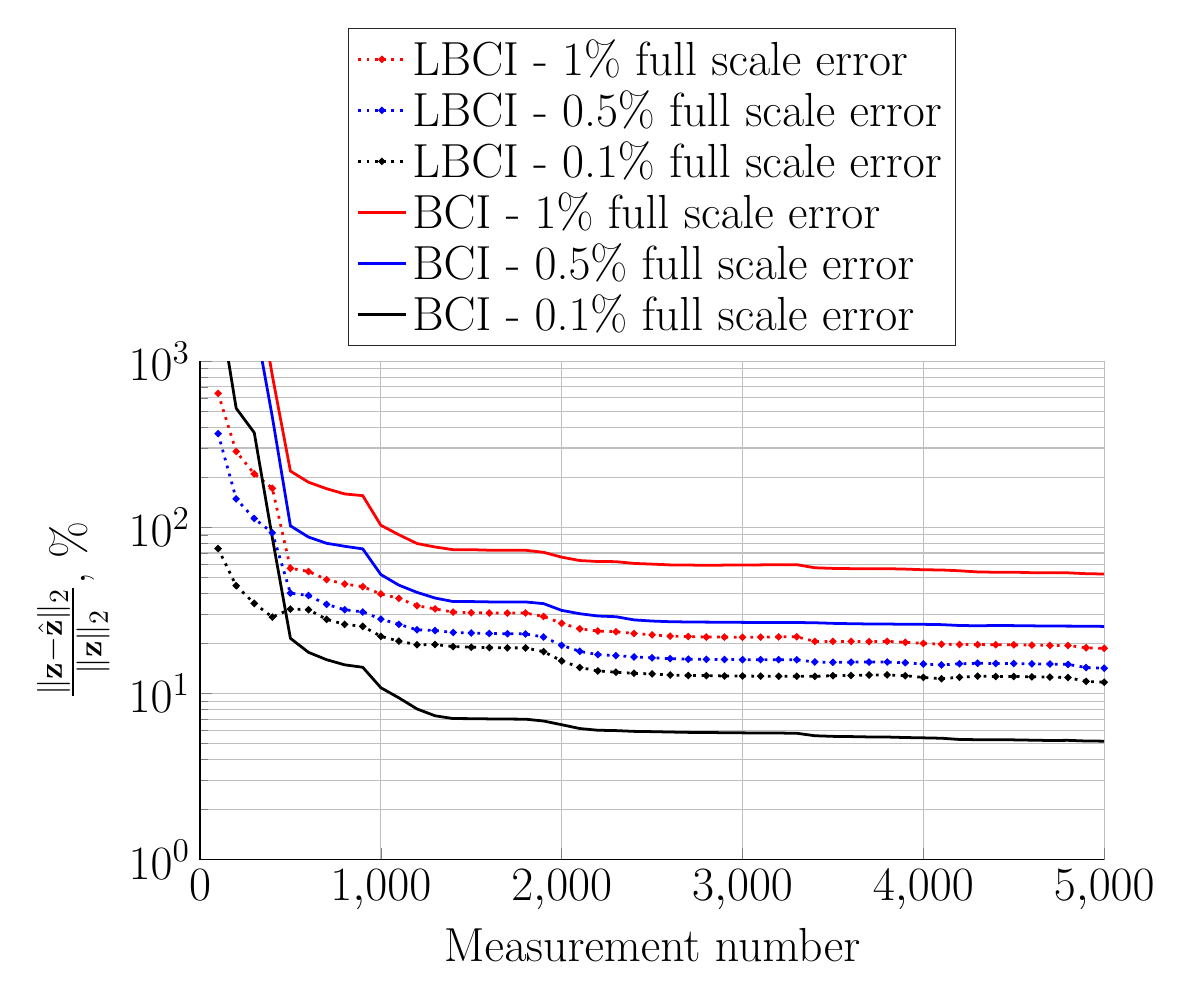
\begin{tikzpicture}

\begin{axis}[%
width=4.521in,
height=2.493in,
at={(0.758in,0.434in)},
scale only axis,
xmin=0,
xmax=5000,
xtick={   0, 1000, 2000, 3000, 4000, 5000},
xlabel={Measurement number},
xmajorgrids,
ymode=log,
ymin=1,
ymax=1000,
yminorticks=true,
ylabel={$\frac{\|\mathbf{z} - \hat{\mathbf{z}}\|_2}{\|\mathbf{z}\|_2}$, \%},
ymajorgrids,
yminorgrids,
axis background/.style={fill=white},
axis x line*=bottom,
axis y line*=left,
legend style={at={(0.5,1.03)},anchor=south,legend cell align=left,align=left,draw=white!15!black},
xlabel style={font=\LARGE},ylabel style={font=\LARGE},legend style={font=\LARGE},ticklabel style={font=\LARGE}
]
\addplot [color=red,dotted,line width=1.0pt,mark size=0.7pt,mark=*,mark options={solid}]
  table[row sep=crcr]{%
100	638.949193481054\\
200	285.70632182257\\
300	209.502339854108\\
400	171.638806921245\\
500	56.645261210907\\
600	54.22432967775\\
700	48.4070108550094\\
800	45.5579631046186\\
900	43.9265013147077\\
1000	39.6900200621635\\
1100	37.3139967910915\\
1200	33.7202706964587\\
1300	32.2708677517544\\
1400	30.8519306407674\\
1500	30.6299745994681\\
1600	30.4741274960733\\
1700	30.4411214252344\\
1800	30.4765370150899\\
1900	29.0628210361043\\
2000	26.4273624315949\\
2100	24.4719832958088\\
2200	23.7458857941618\\
2300	23.5066633297105\\
2400	22.9717915741404\\
2500	22.5405706381273\\
2600	22.1226461839415\\
2700	22.0209644511223\\
2800	21.8561817997409\\
2900	21.8300263708918\\
3000	21.7992148647942\\
3100	21.8198750420406\\
3200	21.8975662766937\\
3300	21.9280484672161\\
3400	20.5566598250784\\
3500	20.5709226407569\\
3600	20.5750150741861\\
3700	20.5289081253015\\
3800	20.5841350806246\\
3900	20.3059484817058\\
4000	20.0412008661088\\
4100	19.7646851911023\\
4200	19.7248735737716\\
4300	19.6916455272616\\
4400	19.6390876030231\\
4500	19.6102477112483\\
4600	19.5229409113847\\
4700	19.4589219229\\
4800	19.4507801909066\\
4900	18.8390541766195\\
5000	18.6845331429238\\
};
\addlegendentry{LBCI - 1\% full scale error};

\addplot [color=blue,dotted,line width=1.0pt,mark size=0.7pt,mark=*,mark options={solid}]
  table[row sep=crcr]{%
100	365.948825420284\\
200	148.216446076282\\
300	112.82942755769\\
400	92.6660881577041\\
500	40.1555990892812\\
600	38.8016657747387\\
700	34.362425175556\\
800	31.9028270853374\\
900	30.9455346352107\\
1000	28.0279998990404\\
1100	26.053396529023\\
1200	24.1610712800741\\
1300	23.9164814349801\\
1400	23.2776564430657\\
1500	23.1007184966155\\
1600	22.9496166699504\\
1700	22.8789805796042\\
1800	22.8170153791079\\
1900	21.8639913285255\\
2000	19.477866340094\\
2100	17.9227592133653\\
2200	17.1375749638645\\
2300	16.8926394652853\\
2400	16.5999628494894\\
2500	16.3933460694156\\
2600	16.1966786578198\\
2700	16.0862140966498\\
2800	16.0565275103474\\
2900	16.0020972844761\\
3000	15.9774325053264\\
3100	15.9694056087035\\
3200	15.9742574063977\\
3300	15.9453833135101\\
3400	15.4657982888896\\
3500	15.3954911357374\\
3600	15.4315000387376\\
3700	15.4603364027782\\
3800	15.4576722731547\\
3900	15.3018064174461\\
4000	15.0390875342421\\
4100	14.8501237659851\\
4200	15.0801491176738\\
4300	15.1959547847747\\
4400	15.1534624825223\\
4500	15.1401647686803\\
4600	15.0874400903603\\
4700	15.029286036236\\
4800	14.9565018376587\\
4900	14.325497747777\\
5000	14.1980293385826\\
};
\addlegendentry{LBCI - 0.5\% full scale error};

\addplot [color=black,dotted,line width=1.0pt,mark size=0.7pt,mark=*,mark options={solid}]
  table[row sep=crcr]{%
100	74.4598834190606\\
200	44.4950743040255\\
300	34.8342380330379\\
400	28.7987073250332\\
500	32.1936194582918\\
600	31.9308237946469\\
700	27.9299784433982\\
800	26.0440102073967\\
900	25.328942043142\\
1000	22.077479335062\\
1100	20.6430801399838\\
1200	19.6388477630566\\
1300	19.7070865082712\\
1400	19.139488227619\\
1500	18.9882857765568\\
1600	18.8551996439041\\
1700	18.8153744934514\\
1800	18.7979378498159\\
1900	17.8512708972745\\
2000	15.6959684149122\\
2100	14.3415927643204\\
2200	13.6530117410485\\
2300	13.4285744595613\\
2400	13.224660233667\\
2500	13.1144657761498\\
2600	12.9189365193015\\
2700	12.8116020666747\\
2800	12.8059658557099\\
2900	12.741825074648\\
3000	12.730315460627\\
3100	12.7014160326678\\
3200	12.6958870656686\\
3300	12.7000573127662\\
3400	12.6847533920869\\
3500	12.7920922286813\\
3600	12.8356589584009\\
3700	12.9141790563003\\
3800	12.9371800409294\\
3900	12.786776324107\\
4000	12.4876544206742\\
4100	12.2599982874187\\
4200	12.5216743294418\\
4300	12.7023157184054\\
4400	12.6564170330362\\
4500	12.6506955677774\\
4600	12.6000811421575\\
4700	12.5400349844273\\
4800	12.4662420549318\\
4900	11.8096026473679\\
5000	11.6825148899311\\
};
\addlegendentry{LBCI - 0.1\% full scale error};

\addplot [color=red,solid,line width=1.0pt]
  table[row sep=crcr]{%
100	22728.0844401917\\
200	5118.69657000351\\
300	3536.99850914306\\
400	816.769790166386\\
500	217.789962578717\\
600	186.673358272156\\
700	170.588712436484\\
800	158.672266693795\\
900	154.945990194417\\
1000	102.812960987144\\
1100	90.0903675033844\\
1200	79.8235730543928\\
1300	76.0952811801202\\
1400	73.2939001233863\\
1500	73.3105008058256\\
1600	72.7745763727444\\
1700	72.7783815896182\\
1800	72.718031543639\\
1900	70.6605592162223\\
2000	66.0800688049927\\
2100	63.0546347055478\\
2200	62.2194878973759\\
2300	62.0956124039623\\
2400	60.6097719919569\\
2500	60.0059486729373\\
2600	59.3725361804331\\
2700	59.273596157382\\
2800	58.9970650417395\\
2900	59.2004854022767\\
3000	59.2540643803915\\
3100	59.3824432036232\\
3200	59.5270961745916\\
3300	59.5457679559992\\
3400	57.0456483739896\\
3500	56.5590202126003\\
3600	56.3618548265959\\
3700	56.3310515498867\\
3800	56.3326145456274\\
3900	56.0118499285963\\
4000	55.4987848173866\\
4100	55.3352463267593\\
4200	54.7210962583346\\
4300	53.8589408369959\\
4400	53.6297037181513\\
4500	53.6839536356162\\
4600	53.2751694592901\\
4700	53.2522253135632\\
4800	53.177736128386\\
4900	52.5670815106881\\
5000	52.3268073688193\\
};
\addlegendentry{BCI - 1\% full scale error};

\addplot [color=blue,solid,line width=1.0pt]
  table[row sep=crcr]{%
100	11400.6317104915\\
200	2709.11003762981\\
300	1837.480807797\\
400	460.735052239631\\
500	102.005394167206\\
600	87.2906130185545\\
700	80.0915493937165\\
800	76.8472619532403\\
900	74.1173835937968\\
1000	51.9491088048463\\
1100	44.8245611687652\\
1200	40.5784875779692\\
1300	37.5024040866603\\
1400	35.7216733221953\\
1500	35.7193452101075\\
1600	35.5593681721333\\
1700	35.5168223438536\\
1800	35.5311590526479\\
1900	34.7140095542001\\
2000	31.6135326665586\\
2100	30.1820496229043\\
2200	29.251150624789\\
2300	28.9584491275208\\
2400	27.7120685560186\\
2500	27.2715114539494\\
2600	27.0170947009927\\
2700	26.9242291975569\\
2800	26.8678826767531\\
2900	26.8440375438859\\
3000	26.772186808124\\
3100	26.7609659888137\\
3200	26.7669739770353\\
3300	26.7189769781261\\
3400	26.6314209655037\\
3500	26.4145706764439\\
3600	26.281180847016\\
3700	26.18937750428\\
3800	26.1581314055083\\
3900	26.086201997588\\
4000	26.0601240884831\\
4100	25.9459986670809\\
4200	25.6442362748963\\
4300	25.5423909233786\\
4400	25.6431195654694\\
4500	25.5931984861965\\
4600	25.5147322817117\\
4700	25.4599795184458\\
4800	25.4167488602764\\
4900	25.4113724076065\\
5000	25.3137359321453\\
};
\addlegendentry{BCI - 0.5\% full scale error};

\addplot [color=black,solid,line width=1.0pt]
  table[row sep=crcr]{%
100	2426.97935227751\\
200	520.097429495387\\
300	370.627433664178\\
400	86.4088147076159\\
500	21.4660738897338\\
600	17.6791178477347\\
700	15.9634979839217\\
800	14.8705928411826\\
900	14.3726130409558\\
1000	10.8271106697378\\
1100	9.40872402129834\\
1200	8.06864024640509\\
1300	7.34031789104499\\
1400	7.06138614146183\\
1500	7.05484216150573\\
1600	7.0294981712566\\
1700	7.01212772537375\\
1800	7.00416054756797\\
1900	6.82498779889169\\
2000	6.48510124758661\\
2100	6.15065684701161\\
2200	6.00827285737952\\
2300	5.97754929288951\\
2400	5.9144943049684\\
2500	5.89186642858549\\
2600	5.85979970044402\\
2700	5.83257088974041\\
2800	5.82381641579081\\
2900	5.8059225153119\\
3000	5.79328015943364\\
3100	5.78378652643428\\
3200	5.778141003319\\
3300	5.76138406166361\\
3400	5.56721982716132\\
3500	5.51920557437916\\
3600	5.50204025657614\\
3700	5.47477625359662\\
3800	5.46857327003434\\
3900	5.43009535981615\\
4000	5.40738490087627\\
4100	5.37831097108823\\
4200	5.28639416421409\\
4300	5.27038746815866\\
4400	5.2594982138701\\
4500	5.25765191351608\\
4600	5.23462274053984\\
4700	5.2121104596335\\
4800	5.22313758218916\\
4900	5.1755789476994\\
5000	5.1637319100943\\
};
\addlegendentry{BCI - 0.1\% full scale error};

\end{axis}
\end{tikzpicture}%
\end{document}
\end{adjustbox}
\end{subfigure}
\begin{subfigure}{0.33\linewidth}
\centering
\begin{adjustbox}{width=1\columnwidth}
% This file was created by matlab2tikz.
%
%The latest updates can be retrieved from
%  http://www.mathworks.com/matlabcentral/fileexchange/22022-matlab2tikz-matlab2tikz
%where you can also make suggestions and rate matlab2tikz.
%
\documentclass[tikz]{standalone}
\usepackage[T1]{fontenc}
\usepackage[utf8]{inputenc}
\usepackage{pgfplots}
\usepackage{grffile}
\pgfplotsset{compat=newest}
\usetikzlibrary{plotmarks}
\usepgfplotslibrary{patchplots}
\usepackage{amsmath}

\begin{document}
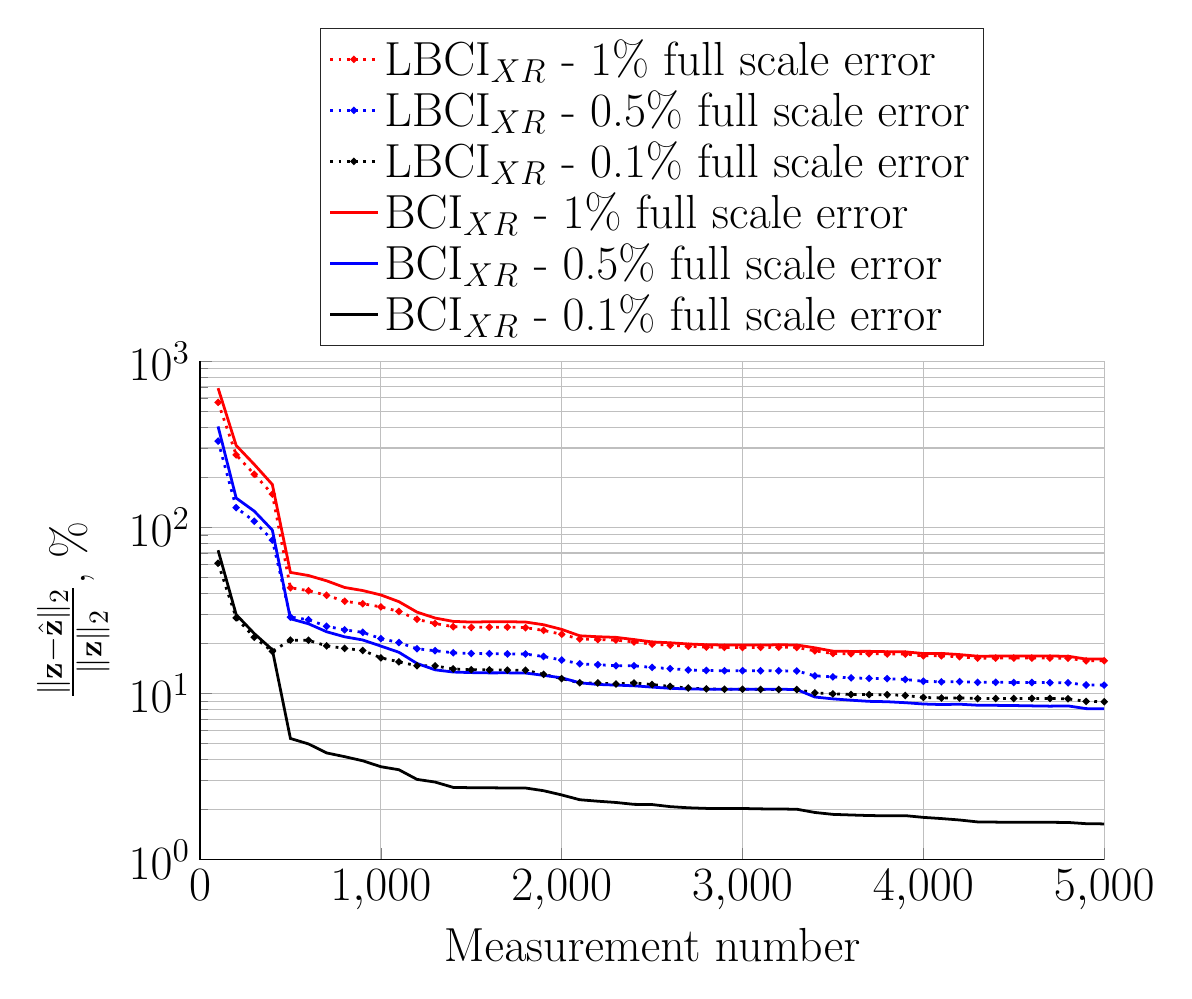
\begin{tikzpicture}

\begin{axis}[%
width=4.521in,
height=2.493in,
at={(0.758in,0.434in)},
scale only axis,
xmin=0,
xmax=5000,
xtick={   0, 1000, 2000, 3000, 4000, 5000},
xlabel={Measurement number},
xmajorgrids,
ymode=log,
ymin=1,
ymax=1000,
yminorticks=true,
ylabel={$\frac{\|\mathbf{z} - \hat{\mathbf{z}}\|_2}{\|\mathbf{z}\|_2}$, \%},
ymajorgrids,
yminorgrids,
axis background/.style={fill=white},
axis x line*=bottom,
axis y line*=left,
legend style={at={(0.5,1.03)},anchor=south,legend cell align=left,align=left,draw=white!15!black},
xlabel style={font=\LARGE},ylabel style={font=\LARGE},legend style={font=\LARGE},ticklabel style={font=\LARGE}
]
\addplot [color=red,dotted,line width=1.0pt,mark size=0.7pt,mark=*,mark options={solid}]
  table[row sep=crcr]{%
100	564.481923572343\\
200	272.484646683434\\
300	208.426318945265\\
400	158.213670454915\\
500	43.2530423217083\\
600	41.5182412254465\\
700	38.9661632298446\\
800	35.8667829694198\\
900	34.6453567193563\\
1000	33.1857591055094\\
1100	31.1448505693434\\
1200	27.9294712318906\\
1300	26.3580797869923\\
1400	25.2236408437764\\
1500	24.9756551590762\\
1600	25.0349164236565\\
1700	25.0712026123535\\
1800	24.886564853032\\
1900	23.9468278266095\\
2000	22.7014139042234\\
2100	21.2480197058099\\
2200	21.0848721371781\\
2300	20.9468040563461\\
2400	20.4269987914412\\
2500	19.8025716616455\\
2600	19.5042199594777\\
2700	19.2122754282362\\
2800	19.0071690887514\\
2900	18.935948398865\\
3000	18.9203080737734\\
3100	18.9171750201994\\
3200	18.9611118308726\\
3300	18.9235284080245\\
3400	18.042555271127\\
3500	17.3935526311081\\
3600	17.3417739884359\\
3700	17.3415275499434\\
3800	17.2870452840383\\
3900	17.2456765872908\\
4000	16.8401098422829\\
4100	16.8408153178072\\
4200	16.6176224272498\\
4300	16.3100484947216\\
4400	16.3282373326122\\
4500	16.3218421831683\\
4600	16.3411522434454\\
4700	16.3294078129004\\
4800	16.3008558277689\\
4900	15.7063308788233\\
5000	15.7273364097281\\
};
\addlegendentry{LBCI$_{XR}$ - 1\% full scale error};

\addplot [color=blue,dotted,line width=1.0pt,mark size=0.7pt,mark=*,mark options={solid}]
  table[row sep=crcr]{%
100	329.925863089506\\
200	131.225400166045\\
300	108.682116612618\\
400	83.7199061694903\\
500	28.8230690447383\\
600	27.7650730482484\\
700	25.3653666029142\\
800	24.1420469821693\\
900	23.319025328123\\
1000	21.3910778175977\\
1100	20.239584858566\\
1200	18.5791291104949\\
1300	18.0789314845483\\
1400	17.5735396804153\\
1500	17.3909669079807\\
1600	17.3511084937124\\
1700	17.2916814906363\\
1800	17.2592605367503\\
1900	16.6891412816758\\
2000	15.8888483539762\\
2100	15.0836693636405\\
2200	14.8880404487268\\
2300	14.6889304580055\\
2400	14.6656772990501\\
2500	14.3434279926162\\
2600	14.1022012744251\\
2700	13.8509685795753\\
2800	13.748250227589\\
2900	13.7058469895653\\
3000	13.7142507230477\\
3100	13.695916710193\\
3200	13.6834915722055\\
3300	13.6562095902141\\
3400	12.7693963651823\\
3500	12.5799418412041\\
3600	12.4092738524808\\
3700	12.3274627923577\\
3800	12.2783319083166\\
3900	12.1352816496976\\
4000	11.8427028028654\\
4100	11.7446357855642\\
4200	11.7806664465127\\
4300	11.6677949714233\\
4400	11.6707793429469\\
4500	11.6511645275251\\
4600	11.6402943665509\\
4700	11.6130716498999\\
4800	11.5847218495694\\
4900	11.2462644521625\\
5000	11.2210900998497\\
};
\addlegendentry{LBCI$_{XR}$ - 0.5\% full scale error};

\addplot [color=black,dotted,line width=1.0pt,mark size=0.7pt,mark=*,mark options={solid}]
  table[row sep=crcr]{%
100	60.7260001960621\\
200	28.5136917518507\\
300	21.776027499514\\
400	17.9259430391606\\
500	20.9443736945084\\
600	20.8758614150486\\
700	19.3364298631374\\
800	18.6803834934567\\
900	18.147328216363\\
1000	16.3891053836993\\
1100	15.4959649300077\\
1200	14.674399916599\\
1300	14.6404061425242\\
1400	14.0457178688981\\
1500	13.9048430723567\\
1600	13.856960474772\\
1700	13.8093330493652\\
1800	13.7762342416552\\
1900	13.0387989871401\\
2000	12.2797144693579\\
2100	11.5930283912766\\
2200	11.5616790113835\\
2300	11.403174069441\\
2400	11.5720258998527\\
2500	11.3178370570721\\
2600	11.0260163491567\\
2700	10.7779347486385\\
2800	10.6592282753327\\
2900	10.6051121440769\\
3000	10.6051026734001\\
3100	10.5756435746973\\
3200	10.5599332659085\\
3300	10.5504080690842\\
3400	10.0816336064368\\
3500	9.94396168508698\\
3600	9.86586674722158\\
3700	9.84590160006396\\
3800	9.83298772494378\\
3900	9.7237746939626\\
4000	9.46287268266297\\
4100	9.39366871198762\\
4200	9.40094153031319\\
4300	9.32162687665783\\
4400	9.33169172397399\\
4500	9.32441675808094\\
4600	9.3414630748198\\
4700	9.33513432309673\\
4800	9.28491438338282\\
4900	8.95135307849097\\
5000	8.91797640279913\\
};
\addlegendentry{LBCI$_{XR}$ - 0.1\% full scale error};

\addplot [color=red,solid,line width=1.0pt]
  table[row sep=crcr]{%
100	687.162632312096\\
200	310.581909851338\\
300	238.8564667258\\
400	180.902080862412\\
500	53.4955991216033\\
600	51.2362052694262\\
700	47.625529793001\\
800	43.4151969883932\\
900	41.6042688251828\\
1000	39.1592652954947\\
1100	35.6674632497747\\
1200	30.8666349120025\\
1300	28.4308514040445\\
1400	27.1421605790363\\
1500	26.8893304853057\\
1600	27.0088309173177\\
1700	27.0210911435296\\
1800	26.9021906597949\\
1900	25.909629026642\\
2000	24.2939280348576\\
2100	22.2330831591075\\
2200	21.9430333743929\\
2300	21.7602911615194\\
2400	21.0996757855984\\
2500	20.4152038530171\\
2600	20.1781764715397\\
2700	19.8531190698737\\
2800	19.6471796084147\\
2900	19.5783091473384\\
3000	19.5478853043168\\
3100	19.5685040159804\\
3200	19.6250956269494\\
3300	19.5835760920241\\
3400	18.8266934184721\\
3500	17.9666396640691\\
3600	17.9064595928047\\
3700	17.9216792159022\\
3800	17.8410373739834\\
3900	17.7969598729175\\
4000	17.3979067603842\\
4100	17.4239973806169\\
4200	17.1328370985482\\
4300	16.7613593265288\\
4400	16.7802145012919\\
4500	16.7797938421224\\
4600	16.7930000447739\\
4700	16.7899473869768\\
4800	16.7567820457399\\
4900	16.1031637272547\\
5000	16.1241967612528\\
};
\addlegendentry{BCI$_{XR}$ - 1\% full scale error};

\addplot [color=blue,solid,line width=1.0pt]
  table[row sep=crcr]{%
100	404.1321725797\\
200	149.907145372373\\
300	125.047013550393\\
400	96.2052957147922\\
500	28.1385540829226\\
600	26.2564948383921\\
700	23.5119455154061\\
800	21.9201928831837\\
900	20.9847690368135\\
1000	19.282089588279\\
1100	17.6908447294148\\
1200	15.1549445078433\\
1300	13.8749438847117\\
1400	13.4550865853242\\
1500	13.3511605321021\\
1600	13.2977969667917\\
1700	13.3066388691057\\
1800	13.2644462935719\\
1900	12.8539181640328\\
2000	12.4206026227885\\
2100	11.5917373605801\\
2200	11.3306951547318\\
2300	11.2297673687889\\
2400	11.1164398891805\\
2500	10.9186750128686\\
2600	10.7415289122971\\
2700	10.6389535941284\\
2800	10.6098105589105\\
2900	10.5977162124967\\
3000	10.6166732692131\\
3100	10.5963378544181\\
3200	10.6086783421659\\
3300	10.5527427481681\\
3400	9.51993532860792\\
3500	9.27804611209175\\
3600	9.10848054090651\\
3700	8.96508734171332\\
3800	8.91796616030325\\
3900	8.79864730528896\\
4000	8.64131244856672\\
4100	8.5756305258051\\
4200	8.61643132577958\\
4300	8.49587863563992\\
4400	8.48170845152912\\
4500	8.45965768252504\\
4600	8.42125014536799\\
4700	8.38815775564816\\
4800	8.41531848948757\\
4900	8.10499014595432\\
5000	8.0932767770725\\
};
\addlegendentry{BCI$_{XR}$ - 0.5\% full scale error};

\addplot [color=black,solid,line width=1.0pt]
  table[row sep=crcr]{%
100	72.7195490887134\\
200	29.8355381810924\\
300	22.9326955663768\\
400	18.3217119954536\\
500	5.35976617652142\\
600	4.9693423911885\\
700	4.38776740234361\\
800	4.16555527409481\\
900	3.93519315037906\\
1000	3.62564767137419\\
1100	3.47519256870061\\
1200	3.04084066537432\\
1300	2.93004121813041\\
1400	2.72205052231501\\
1500	2.70965158616435\\
1600	2.70543137930573\\
1700	2.70071097718423\\
1800	2.69858839141467\\
1900	2.59940062923238\\
2000	2.45141671070456\\
2100	2.2937077370773\\
2200	2.24764004009169\\
2300	2.20854708761487\\
2400	2.1515491404239\\
2500	2.14573839185848\\
2600	2.08475565438333\\
2700	2.05198197165185\\
2800	2.03458243419119\\
2900	2.02860411526808\\
3000	2.03171625846985\\
3100	2.02131144427194\\
3200	2.01716151247194\\
3300	2.01121763815109\\
3400	1.9230171551157\\
3500	1.87301500214421\\
3600	1.85730571413849\\
3700	1.84271459294255\\
3800	1.83633521278918\\
3900	1.84035199739431\\
4000	1.79664021587933\\
4100	1.76738193462632\\
4200	1.73275273990007\\
4300	1.68679283100553\\
4400	1.68237342382349\\
4500	1.67865029296265\\
4600	1.67946483079034\\
4700	1.6775715993085\\
4800	1.67466385165876\\
4900	1.64625904730214\\
5000	1.64095509018859\\
};
\addlegendentry{BCI$_{XR}$ - 0.1\% full scale error};

\end{axis}
\end{tikzpicture}%
\end{document}
\end{adjustbox}
\end{subfigure}
\begin{subfigure}{0.33\linewidth}
\centering
\begin{adjustbox}{width=1\columnwidth}
% This file was created by matlab2tikz.
%
%The latest updates can be retrieved from
%  http://www.mathworks.com/matlabcentral/fileexchange/22022-matlab2tikz-matlab2tikz
%where you can also make suggestions and rate matlab2tikz.
%
\documentclass[tikz]{standalone}
\usepackage[T1]{fontenc}
\usepackage[utf8]{inputenc}
\usepackage{pgfplots}
\usepackage{grffile}
\pgfplotsset{compat=newest}
\usetikzlibrary{plotmarks}
\usepgfplotslibrary{patchplots}
\usepackage{amsmath}

\begin{document}
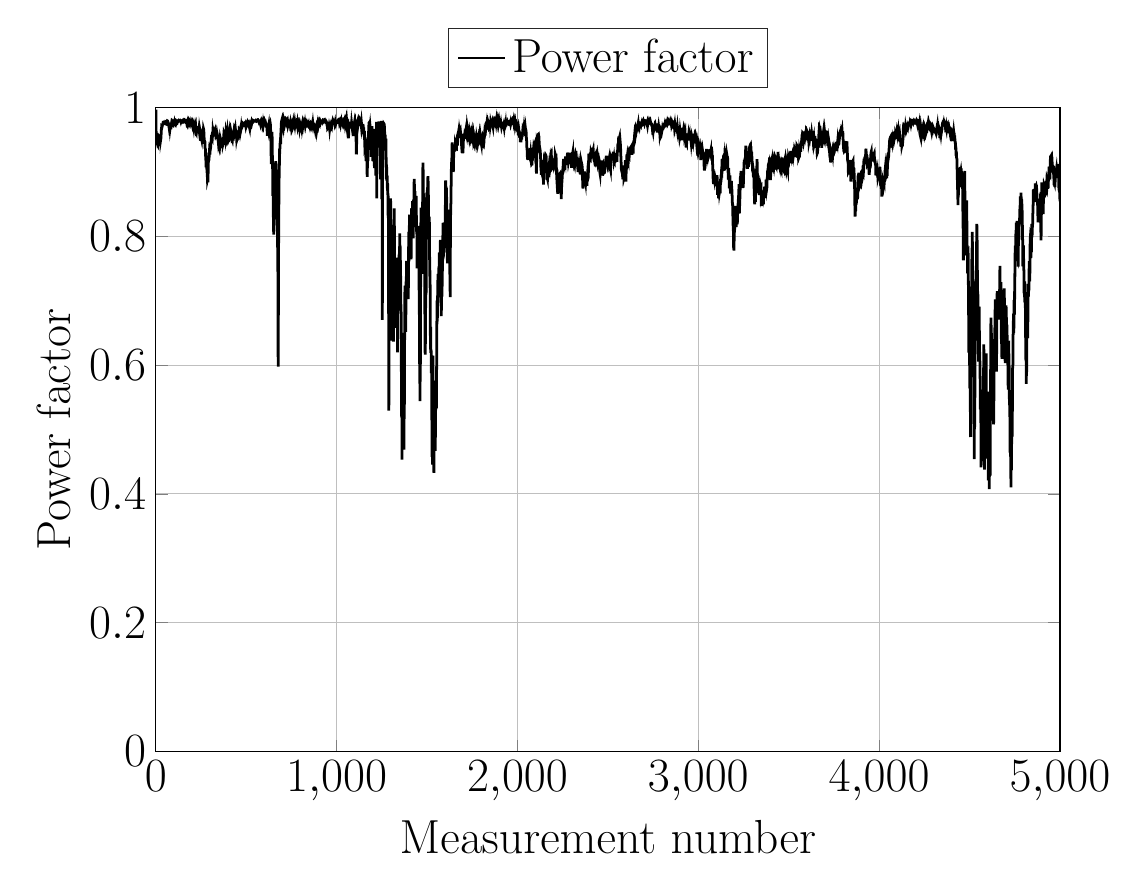
\begin{tikzpicture}

\begin{axis}[%
width=4.521in,
height=3.219in,
at={(0.758in,0.434in)},
scale only axis,
xmin=0,
xmax=5000,
xtick={   0, 1000, 2000, 3000, 4000, 5000},
xlabel={Measurement number},
xmajorgrids,
ymin=0,
ymax=1,
ylabel={Power factor},
ymajorgrids,
axis background/.style={fill=white},
legend style={at={(0.5,1.03)},anchor=south,legend cell align=left,align=left,draw=white!15!black},
xlabel style={font=\LARGE},ylabel style={font=\LARGE},legend style={font=\LARGE},ticklabel style={font=\LARGE}
]
\addplot [color=black,solid,line width=1.0pt,forget plot]
  table[row sep=crcr]{%
1	0.997004259495801\\
2	0.962085500087199\\
3	0.955330733833589\\
4	0.95583000870724\\
5	0.947697537673708\\
6	0.951209485294064\\
7	0.950147725766689\\
8	0.945813201447307\\
9	0.944426771346652\\
10	0.945291050914637\\
11	0.944475615703556\\
12	0.949537920465603\\
13	0.950516908115429\\
14	0.94978355513802\\
15	0.953891966284113\\
16	0.954644323217025\\
17	0.953827990767938\\
18	0.949827445403425\\
19	0.94734625673488\\
20	0.95187769486887\\
21	0.95773526504413\\
22	0.953892376919487\\
23	0.954002089173623\\
24	0.952827545174092\\
25	0.955491707617817\\
26	0.955512551575455\\
27	0.94951874571385\\
28	0.951331711267227\\
29	0.953459490786163\\
30	0.960591478791183\\
31	0.966428419373809\\
32	0.967043626776505\\
33	0.971966138000047\\
34	0.971784657208473\\
35	0.972178373755379\\
36	0.971356848512516\\
37	0.972581359386795\\
38	0.973924406197923\\
39	0.974122851326296\\
40	0.975693485632007\\
41	0.975495019469873\\
42	0.976818036370448\\
43	0.977453740293068\\
44	0.977725199409554\\
45	0.97779780879695\\
46	0.977681417718602\\
47	0.977491813937866\\
48	0.977172384616925\\
49	0.975948719349971\\
50	0.975552386382414\\
51	0.975236160146525\\
52	0.975185249286379\\
53	0.97501658841383\\
54	0.97681447182223\\
55	0.977895342068554\\
56	0.977724284591543\\
57	0.977140814459484\\
58	0.977035636497284\\
59	0.976684844080851\\
60	0.976246919608408\\
61	0.977286228277888\\
62	0.978287683975953\\
63	0.978784806326059\\
64	0.979505658258968\\
65	0.979335425339207\\
66	0.979175805161512\\
67	0.978285354647429\\
68	0.977396764449152\\
69	0.975996658853483\\
70	0.973963798171539\\
71	0.973069433034206\\
72	0.972850055243157\\
73	0.970827128061033\\
74	0.972596372141984\\
75	0.974376552365826\\
76	0.974226568162199\\
77	0.97255408890403\\
78	0.970642137421386\\
79	0.967280127537736\\
80	0.969389323433505\\
81	0.968819592677724\\
82	0.968394979032063\\
83	0.968951762276899\\
84	0.97081568796214\\
85	0.972751142286271\\
86	0.973528254104379\\
87	0.975284678414647\\
88	0.974440382217352\\
89	0.97600147296866\\
90	0.977007888621275\\
91	0.976334007149345\\
92	0.97552556130867\\
93	0.97458448911799\\
94	0.974087931035193\\
95	0.973744247100369\\
96	0.973422971639521\\
97	0.975161072500993\\
98	0.976927726626948\\
99	0.976484487908057\\
100	0.974814014953759\\
101	0.975279981079628\\
102	0.976440386271532\\
103	0.974334893103281\\
104	0.973563556576961\\
105	0.973501809336581\\
106	0.975697839136599\\
107	0.975253294682772\\
108	0.974663592609015\\
109	0.975352908830909\\
110	0.977176553685412\\
111	0.977936785048168\\
112	0.978912249629755\\
113	0.978534536901781\\
114	0.97709488643857\\
115	0.97803032383336\\
116	0.977572538071297\\
117	0.978533463645508\\
118	0.979372247122391\\
119	0.979459253979012\\
120	0.979215572843827\\
121	0.979322850513133\\
122	0.978606836537799\\
123	0.979342424414937\\
124	0.979651457296618\\
125	0.979928136071944\\
126	0.979440492778496\\
127	0.979754651486408\\
128	0.979884224400295\\
129	0.979375418691526\\
130	0.979268579045572\\
131	0.979542625600239\\
132	0.979624709993825\\
133	0.97958662750911\\
134	0.979722366403391\\
135	0.979956963803809\\
136	0.979540541038404\\
137	0.979543506587283\\
138	0.978929797574068\\
139	0.9779626341566\\
140	0.978848074263184\\
141	0.978586355887966\\
142	0.97880891620266\\
143	0.978480637574209\\
144	0.979295963427528\\
145	0.979498443743644\\
146	0.979033043034659\\
147	0.979651405589772\\
148	0.979689146298204\\
149	0.979895365449869\\
150	0.979403295915238\\
151	0.979851324743748\\
152	0.979232418745477\\
153	0.978834832299038\\
154	0.979436585432642\\
155	0.979567214991476\\
156	0.97990610500525\\
157	0.979383296247609\\
158	0.979671079754848\\
159	0.979406445911521\\
160	0.979842718731312\\
161	0.97916149714353\\
162	0.978662357447038\\
163	0.979064151878464\\
164	0.979011103080068\\
165	0.979078432913774\\
166	0.97924553341052\\
167	0.978794818459743\\
168	0.978529101599445\\
169	0.978250937227177\\
170	0.978300770528725\\
171	0.976551366098099\\
172	0.977266897380619\\
173	0.975703177195552\\
174	0.974720722884536\\
175	0.976136108277743\\
176	0.976006606351949\\
177	0.977284540132788\\
178	0.975870607172832\\
179	0.975811359679479\\
180	0.976943238981298\\
181	0.978093235912004\\
182	0.976912357037097\\
183	0.978724071893731\\
184	0.978377870369609\\
185	0.979212554582241\\
186	0.979173613176576\\
187	0.978205382186085\\
188	0.97890250503846\\
189	0.977385906904453\\
190	0.976324035943415\\
191	0.977739963993948\\
192	0.97898529737752\\
193	0.979244357750292\\
194	0.979388947104317\\
195	0.978644751722599\\
196	0.977304913799867\\
197	0.977418247558758\\
198	0.978172965881364\\
199	0.977175806492294\\
200	0.97492667794376\\
201	0.973732946196006\\
202	0.976264861283677\\
203	0.976769719435177\\
204	0.977355470207067\\
205	0.978296348759962\\
206	0.977425462866745\\
207	0.976109755771697\\
208	0.974346799826136\\
209	0.97266167549769\\
210	0.97052814205426\\
211	0.973289457497484\\
212	0.973228380966314\\
213	0.97311038339622\\
214	0.973088403542331\\
215	0.971337078504937\\
216	0.970626378077438\\
217	0.972229550702111\\
218	0.970367173609657\\
219	0.969325589188778\\
220	0.967411143501241\\
221	0.96884784766834\\
222	0.964099215124133\\
223	0.963174643182468\\
224	0.965453599269096\\
225	0.964437665129631\\
226	0.968397504518184\\
227	0.96850897928643\\
228	0.966158943802257\\
229	0.960128986437294\\
230	0.964850922780475\\
231	0.961076590354996\\
232	0.964583242436725\\
233	0.964586781555759\\
234	0.960736667003061\\
235	0.967283297999615\\
236	0.967487535035713\\
237	0.965389796093387\\
238	0.965087487135543\\
239	0.967277983731285\\
240	0.964962533446491\\
241	0.966898499720252\\
242	0.961077883006057\\
243	0.96694894280685\\
244	0.965358019645728\\
245	0.959774564178173\\
246	0.956461577838436\\
247	0.952301778783729\\
248	0.954433915451136\\
249	0.948553447597876\\
250	0.954277256305801\\
251	0.955361291366873\\
252	0.952549395605051\\
253	0.951689622509145\\
254	0.950322655527579\\
255	0.954185190893729\\
256	0.954756754957811\\
257	0.950101542675794\\
258	0.957424758093786\\
259	0.95821451677895\\
260	0.956286260825967\\
261	0.963651111318809\\
262	0.960396604640943\\
263	0.962000796852183\\
264	0.966958964685126\\
265	0.965857367107823\\
266	0.962642408898721\\
267	0.956237951996438\\
268	0.949328482721095\\
269	0.948856330182527\\
270	0.943650313333767\\
271	0.947215698052191\\
272	0.946670891556756\\
273	0.936780789544654\\
274	0.936240230119512\\
275	0.934661699039717\\
276	0.922001126257862\\
277	0.921011556296932\\
278	0.907118437806313\\
279	0.922583338450816\\
280	0.912904549576639\\
281	0.911739198239489\\
282	0.905432189605268\\
283	0.905291986586318\\
284	0.89911293560969\\
285	0.895555620326173\\
286	0.888413568510116\\
287	0.889727718144684\\
288	0.895708112560649\\
289	0.883681332374162\\
290	0.908659259448401\\
291	0.915316513197283\\
292	0.921741504609862\\
293	0.921161234390866\\
294	0.917586844851372\\
295	0.922247085427479\\
296	0.926704762505553\\
297	0.932715347712008\\
298	0.937257479859774\\
299	0.936550388033514\\
300	0.927117446009277\\
301	0.935611180834603\\
302	0.937011369860521\\
303	0.937058403244522\\
304	0.939590022824596\\
305	0.946320830349797\\
306	0.947240856902622\\
307	0.95190404916924\\
308	0.95205082695868\\
309	0.957478411348122\\
310	0.952481340871321\\
311	0.954937768173791\\
312	0.954371656199521\\
313	0.953461681046737\\
314	0.957601759470872\\
315	0.957952230453941\\
316	0.963194757977631\\
317	0.961378630595311\\
318	0.962546527296206\\
319	0.963759736107571\\
320	0.962657098668632\\
321	0.962039727365631\\
322	0.966531506890365\\
323	0.963535245445402\\
324	0.964087433513492\\
325	0.965077735115216\\
326	0.965649816202242\\
327	0.961958512406214\\
328	0.960041091095301\\
329	0.958994596244406\\
330	0.96053334962262\\
331	0.958118896003133\\
332	0.95885050572926\\
333	0.954262592041226\\
334	0.958282508238861\\
335	0.958422289155723\\
336	0.962971057727165\\
337	0.958127710260598\\
338	0.952972040096609\\
339	0.955382624989498\\
340	0.951117215745678\\
341	0.955491101371163\\
342	0.953800749031619\\
343	0.954738086562736\\
344	0.953379359401008\\
345	0.95021488900748\\
346	0.946870562021059\\
347	0.948649119892563\\
348	0.942126914111863\\
349	0.940920763882488\\
350	0.946966570251177\\
351	0.946380512904599\\
352	0.946659855274067\\
353	0.943122021280342\\
354	0.945969695633514\\
355	0.944119085066758\\
356	0.947512518688277\\
357	0.952296930340595\\
358	0.951099058115294\\
359	0.94988081874392\\
360	0.944774205320729\\
361	0.947669988550128\\
362	0.953431053735424\\
363	0.947427345274723\\
364	0.946998820762146\\
365	0.93916722634655\\
366	0.938983747488147\\
367	0.944260542460292\\
368	0.947440096876862\\
369	0.950338590090171\\
370	0.945882086218322\\
371	0.942245573502436\\
372	0.943447932055008\\
373	0.947703350585268\\
374	0.948213148438055\\
375	0.952638945571828\\
376	0.956709113713259\\
377	0.960484956923567\\
378	0.959662639342399\\
379	0.956956564235595\\
380	0.950675576227884\\
381	0.955786978451236\\
382	0.958124459602582\\
383	0.958525494655618\\
384	0.95504790418149\\
385	0.95260168090036\\
386	0.95546021431786\\
387	0.957246106176362\\
388	0.961323945208123\\
389	0.959614144993668\\
390	0.957809356324793\\
391	0.96186853264652\\
392	0.964730333564062\\
393	0.960459778352078\\
394	0.95857304845454\\
395	0.955854584003209\\
396	0.959713900689303\\
397	0.962661468399136\\
398	0.960230568567008\\
399	0.955682247313373\\
400	0.954858360120042\\
401	0.951534644507902\\
402	0.948633173668596\\
403	0.94928603517216\\
404	0.946860813253397\\
405	0.952721629959737\\
406	0.955572453676309\\
407	0.960254705140525\\
408	0.962291519600249\\
409	0.959680905362824\\
410	0.958644175210501\\
411	0.959983174141958\\
412	0.964465278266218\\
413	0.963417035276871\\
414	0.961850252908396\\
415	0.963992827647495\\
416	0.962459755723493\\
417	0.961088013480368\\
418	0.958028580342444\\
419	0.951780050767675\\
420	0.954437797938931\\
421	0.953397028692263\\
422	0.95022877854862\\
423	0.950620780693547\\
424	0.94968197140355\\
425	0.952564636548638\\
426	0.957093394848791\\
427	0.957068795095999\\
428	0.957799444692601\\
429	0.959402615564845\\
430	0.961410815615257\\
431	0.962733759293746\\
432	0.962380976823834\\
433	0.96467906204082\\
434	0.963453282334907\\
435	0.961505564408719\\
436	0.963222510350786\\
437	0.964962312810563\\
438	0.963956723768718\\
439	0.966271275699851\\
440	0.967849077713864\\
441	0.96537167172746\\
442	0.963940983758578\\
443	0.958772609611789\\
444	0.958689769699636\\
445	0.954332843053443\\
446	0.95788288410156\\
447	0.952980094918375\\
448	0.954754488912472\\
449	0.960207582632135\\
450	0.960525371669393\\
451	0.954561265148734\\
452	0.955001322177108\\
453	0.96036579703117\\
454	0.957938885297036\\
455	0.959281005898124\\
456	0.960588009375014\\
457	0.961738468651629\\
458	0.961596224200425\\
459	0.960109873839714\\
460	0.961694612269252\\
461	0.965565533933433\\
462	0.96510324528683\\
463	0.964191582830216\\
464	0.962452717613957\\
465	0.963364868517337\\
466	0.965144560633902\\
467	0.965592373192777\\
468	0.966911923064394\\
469	0.962808627530708\\
470	0.96423338900371\\
471	0.966228282197831\\
472	0.968676569985933\\
473	0.970830168928918\\
474	0.968828928799187\\
475	0.969911282041402\\
476	0.972439333510169\\
477	0.971794991941738\\
478	0.971403568029092\\
479	0.972586347344555\\
480	0.974785764386457\\
481	0.976101475040229\\
482	0.975847337808773\\
483	0.975596003535012\\
484	0.974965154277208\\
485	0.974306490606806\\
486	0.972655336486203\\
487	0.971978346848557\\
488	0.971931800349947\\
489	0.972225202801945\\
490	0.974008971344777\\
491	0.97565904317714\\
492	0.976272691544656\\
493	0.976654713782045\\
494	0.976895846749854\\
495	0.975583702316924\\
496	0.97425728483196\\
497	0.972654991494774\\
498	0.970943797684983\\
499	0.97230563669256\\
500	0.974067175930875\\
501	0.973379651996475\\
502	0.974703010065581\\
503	0.975597722683038\\
504	0.975675697108764\\
505	0.974867939724354\\
506	0.975859043306348\\
507	0.974646465979242\\
508	0.974511083763264\\
509	0.975208385893995\\
510	0.974128158617011\\
511	0.974570834497566\\
512	0.976392027443718\\
513	0.977001140773396\\
514	0.977306162427505\\
515	0.976121551498511\\
516	0.974614813319944\\
517	0.971285574454105\\
518	0.969420262046376\\
519	0.968176153955455\\
520	0.97237436716858\\
521	0.971806221388523\\
522	0.96979015360241\\
523	0.971665008338568\\
524	0.973337127757524\\
525	0.972814381511202\\
526	0.974377365809396\\
527	0.976188535614405\\
528	0.975956853299416\\
529	0.977836389412754\\
530	0.978866116064689\\
531	0.977945936997102\\
532	0.976481285738259\\
533	0.977681877982379\\
534	0.978499072329032\\
535	0.979239701400136\\
536	0.979351085089414\\
537	0.97825862089347\\
538	0.978131646265355\\
539	0.978985317046255\\
540	0.978635898549783\\
541	0.979065671717676\\
542	0.978923752242044\\
543	0.978913955118649\\
544	0.979311336528015\\
545	0.979103203306547\\
546	0.979114275245989\\
547	0.979005197810975\\
548	0.979242504996174\\
549	0.979322132790368\\
550	0.979286205221397\\
551	0.979601998625133\\
552	0.979016367207531\\
553	0.978873009245366\\
554	0.979150259655726\\
555	0.978902154935756\\
556	0.978773886372203\\
557	0.979447966013225\\
558	0.979719530038998\\
559	0.97929561173153\\
560	0.979564261235885\\
561	0.979869459455381\\
562	0.979340448163334\\
563	0.979443888169748\\
564	0.979867471502474\\
565	0.979320403662879\\
566	0.979194764334354\\
567	0.979634732452276\\
568	0.979942070277364\\
569	0.979461600641844\\
570	0.978628004555864\\
571	0.978143649385696\\
572	0.976933404588664\\
573	0.977292182888997\\
574	0.977911546077909\\
575	0.978024964467759\\
576	0.97792507656035\\
577	0.976557640616302\\
578	0.97541763637985\\
579	0.977451364422289\\
580	0.9779429481259\\
581	0.979052986253357\\
582	0.979756872021421\\
583	0.978733853050992\\
584	0.978154436502732\\
585	0.979274281578138\\
586	0.978513315273222\\
587	0.978036952697513\\
588	0.977284149988033\\
589	0.9770269351692\\
590	0.974673249264723\\
591	0.975961581410669\\
592	0.977039761966265\\
593	0.975192232122427\\
594	0.977209162831192\\
595	0.975639081462018\\
596	0.977966868193585\\
597	0.97792610348964\\
598	0.979083146702308\\
599	0.979859038485124\\
600	0.978580861149779\\
601	0.976931330446895\\
602	0.974757441366143\\
603	0.972164055197961\\
604	0.975330418880757\\
605	0.976619036344229\\
606	0.97655512875965\\
607	0.975553730975724\\
608	0.974923272774305\\
609	0.97258086641241\\
610	0.972134584339966\\
611	0.969031624454996\\
612	0.971861451207642\\
613	0.970820556297179\\
614	0.973022716324117\\
615	0.969189540188171\\
616	0.96308123979865\\
617	0.95609957014809\\
618	0.958655508180945\\
619	0.961930601478161\\
620	0.962648749325026\\
621	0.964782975424475\\
622	0.963506288892702\\
623	0.968459070403722\\
624	0.971625861999428\\
625	0.973188296893549\\
626	0.969645769803243\\
627	0.96595888205297\\
628	0.966267908004656\\
629	0.969699042042766\\
630	0.969275046073435\\
631	0.971497622491297\\
632	0.974669341228456\\
633	0.975590818380015\\
634	0.973719417256894\\
635	0.965856858180839\\
636	0.964164612996034\\
637	0.945836508501066\\
638	0.925444654145955\\
639	0.912234348719075\\
640	0.948519754723227\\
641	0.929037955790911\\
642	0.951470745804503\\
643	0.962363492578206\\
644	0.945761961287005\\
645	0.922075696330439\\
646	0.924859308086086\\
647	0.862893955602751\\
648	0.914503009507785\\
649	0.908539108267941\\
650	0.829478010268217\\
651	0.834351201488525\\
652	0.802769113043696\\
653	0.814356515010698\\
654	0.832825588669307\\
655	0.826353677138992\\
656	0.85710153644391\\
657	0.845643634133285\\
658	0.829749006169194\\
659	0.839070609842795\\
660	0.877837993691524\\
661	0.859174527545331\\
662	0.856560552893412\\
663	0.902554876071053\\
664	0.916827346678952\\
665	0.905770670303553\\
666	0.871834985727143\\
667	0.844101862002491\\
668	0.843940061441328\\
669	0.876491331796635\\
670	0.903400827274745\\
671	0.892194114256076\\
672	0.843553456443281\\
673	0.782823523222988\\
674	0.827921971295305\\
675	0.794352263100895\\
676	0.654617729672792\\
677	0.597600679087595\\
678	0.675475132550481\\
679	0.769960981634881\\
680	0.817947392642696\\
681	0.858170464433307\\
682	0.889305039493826\\
683	0.895490887439161\\
684	0.922109626434114\\
685	0.935815818832893\\
686	0.934172325252\\
687	0.939719648691295\\
688	0.946074298747703\\
689	0.947486370647217\\
690	0.953611931258659\\
691	0.943115930274457\\
692	0.961759936543005\\
693	0.965914562928883\\
694	0.972807834865563\\
695	0.9780828673768\\
696	0.979127844227793\\
697	0.975824590677096\\
698	0.975382531566147\\
699	0.971781566074322\\
700	0.975486226854424\\
701	0.977925212565639\\
702	0.979534783627791\\
703	0.977420660283898\\
704	0.977443309099431\\
705	0.977013836458783\\
706	0.973816839764277\\
707	0.976145226229559\\
708	0.974142911095286\\
709	0.976752088961289\\
710	0.978501780989888\\
711	0.977705804020925\\
712	0.979048240359204\\
713	0.979900395799006\\
714	0.978742173065414\\
715	0.979347375221443\\
716	0.976819982526111\\
717	0.978053348628791\\
718	0.977943041184857\\
719	0.976860169908238\\
720	0.977637992751209\\
721	0.977896036669212\\
722	0.976952947024932\\
723	0.979234774327844\\
724	0.979830367059981\\
725	0.978503243356429\\
726	0.979242439558581\\
727	0.978701035308367\\
728	0.97669618811763\\
729	0.977627999164609\\
730	0.975175087293068\\
731	0.972744048158332\\
732	0.973907221743306\\
733	0.971978829556383\\
734	0.971726850479643\\
735	0.975083736551771\\
736	0.977491599123669\\
737	0.977758101631924\\
738	0.978077595009053\\
739	0.977467490737252\\
740	0.975700870478591\\
741	0.975529469441569\\
742	0.971833204187041\\
743	0.975358757362027\\
744	0.976825378611479\\
745	0.97485595460841\\
746	0.97014428449737\\
747	0.970633950026645\\
748	0.966980874910021\\
749	0.967141047219265\\
750	0.967211177213506\\
751	0.966747259876775\\
752	0.964041137972237\\
753	0.964695387138491\\
754	0.968343345593652\\
755	0.973095528164498\\
756	0.975122581923856\\
757	0.974258227658022\\
758	0.971522648913902\\
759	0.972353436492735\\
760	0.97253545354991\\
761	0.974888225758379\\
762	0.972669483009597\\
763	0.9734829163589\\
764	0.97330662007728\\
765	0.972572085754411\\
766	0.973034858273697\\
767	0.971939357057127\\
768	0.974354075623564\\
769	0.976531405931438\\
770	0.974331310341284\\
771	0.976625289620633\\
772	0.977052465116437\\
773	0.976375571051762\\
774	0.975913281699012\\
775	0.976612149377144\\
776	0.975355583874917\\
777	0.974212959618468\\
778	0.973418772046845\\
779	0.975558288462207\\
780	0.976506511527925\\
781	0.975689410227795\\
782	0.974074565829945\\
783	0.972364135723793\\
784	0.974827481393905\\
785	0.972722300541996\\
786	0.971148693008091\\
787	0.972222248098382\\
788	0.968597971967276\\
789	0.968004377023375\\
790	0.970583059573818\\
791	0.970879876480291\\
792	0.970418414985625\\
793	0.970162237144182\\
794	0.970867262267034\\
795	0.968441208268619\\
796	0.970499258111072\\
797	0.972849621691675\\
798	0.971665400716999\\
799	0.97355237044949\\
800	0.972405891322625\\
801	0.970303989616548\\
802	0.966470066944188\\
803	0.970571943175872\\
804	0.970907854864195\\
805	0.9693445631477\\
806	0.970798540323841\\
807	0.97006716952346\\
808	0.971777703395706\\
809	0.973201776998665\\
810	0.96951578425848\\
811	0.9713596357916\\
812	0.97169351621763\\
813	0.970457076824918\\
814	0.972563008013949\\
815	0.97300133126962\\
816	0.973769474170194\\
817	0.975760704484036\\
818	0.977437979213207\\
819	0.978511285213856\\
820	0.977636191219408\\
821	0.978213819352117\\
822	0.977061732995244\\
823	0.977542970005931\\
824	0.975979914731759\\
825	0.974257974596479\\
826	0.976239358876335\\
827	0.974499347366041\\
828	0.976534935085556\\
829	0.977163463377067\\
830	0.978544971248744\\
831	0.978257954251018\\
832	0.97684844538552\\
833	0.976988204553528\\
834	0.977656939090519\\
835	0.976619692512888\\
836	0.97545379877373\\
837	0.976216415695533\\
838	0.975432553855881\\
839	0.976597791700516\\
840	0.976834268135243\\
841	0.975815169684092\\
842	0.973789928250084\\
843	0.973732843461598\\
844	0.97302921559477\\
845	0.97398236112568\\
846	0.971838195914506\\
847	0.971968499762222\\
848	0.97365475100777\\
849	0.972989792537953\\
850	0.971840003788842\\
851	0.972284407049011\\
852	0.971079279415515\\
853	0.972730118338924\\
854	0.973056946988689\\
855	0.974587928666314\\
856	0.975474814364736\\
857	0.976172554243394\\
858	0.975651137905539\\
859	0.973840379796379\\
860	0.973920298141692\\
861	0.974103630168747\\
862	0.972205325314966\\
863	0.97322162449741\\
864	0.973879245258303\\
865	0.974217977014233\\
866	0.975574077709134\\
867	0.973721448604068\\
868	0.972335099770167\\
869	0.974757256777266\\
870	0.972260687394817\\
871	0.971017252190775\\
872	0.972037135036588\\
873	0.972951292780774\\
874	0.972736094286279\\
875	0.973192207298717\\
876	0.972563409898237\\
877	0.972528430890164\\
878	0.970558825713279\\
879	0.970706653326969\\
880	0.967038256337593\\
881	0.965566193938553\\
882	0.968173722658481\\
883	0.969609056953377\\
884	0.971114973681391\\
885	0.97105191210558\\
886	0.970240942008375\\
887	0.971204583048227\\
888	0.969619134893507\\
889	0.970593102109286\\
890	0.969835935626557\\
891	0.966170506499012\\
892	0.968107908015308\\
893	0.9640140659669\\
894	0.967434614180456\\
895	0.969009934083192\\
896	0.971145242241835\\
897	0.973106694502866\\
898	0.971840218419257\\
899	0.973531982928857\\
900	0.97408679185993\\
901	0.975479546204829\\
902	0.976960652943126\\
903	0.975972224418605\\
904	0.97571797555721\\
905	0.975927652441795\\
906	0.975206013276105\\
907	0.977182911481844\\
908	0.976394594784892\\
909	0.977026365082964\\
910	0.978318183312475\\
911	0.977550012763188\\
912	0.978799503187735\\
913	0.979557101006072\\
914	0.979433185984276\\
915	0.978994506153042\\
916	0.978653982765165\\
917	0.978049601245343\\
918	0.978093675935908\\
919	0.979129892596485\\
920	0.979189049126975\\
921	0.978366700054417\\
922	0.979206805389766\\
923	0.979745413021442\\
924	0.97936140080007\\
925	0.979868268820432\\
926	0.979409627961289\\
927	0.978760452042923\\
928	0.979298626214535\\
929	0.979622544803614\\
930	0.97990438035684\\
931	0.979381060802072\\
932	0.979614997597247\\
933	0.979512645918239\\
934	0.979420612886445\\
935	0.978890348211356\\
936	0.979539309219762\\
937	0.978843567944023\\
938	0.978300238686739\\
939	0.977738448899193\\
940	0.977791374880686\\
941	0.978281361858044\\
942	0.978812531344366\\
943	0.978290522966673\\
944	0.97705624044898\\
945	0.976855334392366\\
946	0.975459073239607\\
947	0.973376122924279\\
948	0.971260817729262\\
949	0.971103903120422\\
950	0.967909249887124\\
951	0.968353490970205\\
952	0.970165358617461\\
953	0.971409467122824\\
954	0.972194527978255\\
955	0.972656002157512\\
956	0.973012348157118\\
957	0.971508529517283\\
958	0.970075988894478\\
959	0.97190833680472\\
960	0.970564848935244\\
961	0.970313623993189\\
962	0.967180558326032\\
963	0.969361183943948\\
964	0.969113968548959\\
965	0.970175694009668\\
966	0.967160418992573\\
967	0.966952198149223\\
968	0.97136016204316\\
969	0.9717574146668\\
970	0.972621196930664\\
971	0.974229264670844\\
972	0.975302745416638\\
973	0.974900806254904\\
974	0.973652695209068\\
975	0.976118804070557\\
976	0.977728726022934\\
977	0.978638283076698\\
978	0.979669471565781\\
979	0.978539250637944\\
980	0.979517424023928\\
981	0.979967844062951\\
982	0.979367412661584\\
983	0.978669345668133\\
984	0.978949116558284\\
985	0.979456237704236\\
986	0.979663743214519\\
987	0.978475916153219\\
988	0.977082996505607\\
989	0.977502483883977\\
990	0.975701767370773\\
991	0.976983809546778\\
992	0.974527457515728\\
993	0.975149426477807\\
994	0.976822124041044\\
995	0.977896118361606\\
996	0.978095106223678\\
997	0.976407490732025\\
998	0.977498363991964\\
999	0.977260776706636\\
1000	0.977642921242665\\
1001	0.977702997254054\\
1002	0.978585290186738\\
1003	0.979357014030219\\
1004	0.979635849305027\\
1005	0.978926807868677\\
1006	0.979129565147644\\
1007	0.978609833399513\\
1008	0.979083721222205\\
1009	0.978098095245161\\
1010	0.978306026447478\\
1011	0.978680640020503\\
1012	0.979244383626336\\
1013	0.978638485081217\\
1014	0.977677433237583\\
1015	0.978306034585179\\
1016	0.976102372380197\\
1017	0.976970945881674\\
1018	0.977585413773663\\
1019	0.978902441020234\\
1020	0.978431405047155\\
1021	0.97739868452952\\
1022	0.975676602055676\\
1023	0.9776799745682\\
1024	0.976964552683749\\
1025	0.978202150726291\\
1026	0.975704396235945\\
1027	0.976246553371662\\
1028	0.978189776676907\\
1029	0.978536952708024\\
1030	0.978789349566435\\
1031	0.976356767658705\\
1032	0.975501655340918\\
1033	0.977446112799469\\
1034	0.978201385500708\\
1035	0.976811409891407\\
1036	0.976741373383478\\
1037	0.975642926293383\\
1038	0.97728304044204\\
1039	0.976644431126667\\
1040	0.97700799285396\\
1041	0.978070365316095\\
1042	0.978986138569442\\
1043	0.976902965323885\\
1044	0.977472441500825\\
1045	0.978725778282121\\
1046	0.976920657982155\\
1047	0.974564523123531\\
1048	0.976335367011084\\
1049	0.976405720199261\\
1050	0.978050098140455\\
1051	0.976993025792655\\
1052	0.97868859045917\\
1053	0.976790635823699\\
1054	0.979019951853397\\
1055	0.976884127198549\\
1056	0.978965671577648\\
1057	0.975765035966552\\
1058	0.978115655676628\\
1059	0.978191420741835\\
1060	0.975708199721696\\
1061	0.976732580007259\\
1062	0.977120755024332\\
1063	0.971887246052032\\
1064	0.963831546806452\\
1065	0.952272654211641\\
1066	0.956948865650335\\
1067	0.957483067766418\\
1068	0.968057075568734\\
1069	0.973038176055005\\
1070	0.968573503277235\\
1071	0.972343851760157\\
1072	0.972122067260805\\
1073	0.97160404704522\\
1074	0.967840140052324\\
1075	0.975419935518177\\
1076	0.975419947427555\\
1077	0.972973674986457\\
1078	0.978244339277777\\
1079	0.971198730116992\\
1080	0.971077603763456\\
1081	0.970603357160999\\
1082	0.972595973733117\\
1083	0.976136857800316\\
1084	0.973927078783785\\
1085	0.976793647050843\\
1086	0.971522861268884\\
1087	0.971123153874947\\
1088	0.965459035074224\\
1089	0.962163057242556\\
1090	0.968804864256895\\
1091	0.963600098597531\\
1092	0.955621352290882\\
1093	0.965553340436225\\
1094	0.968983040550223\\
1095	0.97105833696642\\
1096	0.975581414558615\\
1097	0.969413428794995\\
1098	0.975486274831541\\
1099	0.977159089338851\\
1100	0.974826612330544\\
1101	0.976115193938745\\
1102	0.971063442245468\\
1103	0.970768224906126\\
1104	0.974805070629626\\
1105	0.971088235231766\\
1106	0.964690802261078\\
1107	0.964174025208966\\
1108	0.948279052153882\\
1109	0.927483839157307\\
1110	0.947686577287969\\
1111	0.946297307229243\\
1112	0.958681806765981\\
1113	0.9725528383915\\
1114	0.971977747913873\\
1115	0.977860886017427\\
1116	0.978803689168765\\
1117	0.974953926688958\\
1118	0.978997539391575\\
1119	0.976270383594118\\
1120	0.978643817603255\\
1121	0.979926381916897\\
1122	0.978658492103708\\
1123	0.97927185806045\\
1124	0.979915641824396\\
1125	0.978701000161561\\
1126	0.979937915747835\\
1127	0.97903221322528\\
1128	0.979924803459906\\
1129	0.979022946151364\\
1130	0.978896385518744\\
1131	0.978102178896416\\
1132	0.97900374690249\\
1133	0.979045572562027\\
1134	0.977237870759271\\
1135	0.978141043135882\\
1136	0.97498609611992\\
1137	0.977174485040712\\
1138	0.97402902950075\\
1139	0.972810144748903\\
1140	0.969242451797689\\
1141	0.971017653341883\\
1142	0.969639839898339\\
1143	0.96586668739397\\
1144	0.969108959178011\\
1145	0.971160660164392\\
1146	0.974496401846981\\
1147	0.971017373538443\\
1148	0.964641057465506\\
1149	0.961783233408301\\
1150	0.969172803042934\\
1151	0.962693037695425\\
1152	0.959586154571679\\
1153	0.961716052005455\\
1154	0.963596372208458\\
1155	0.957545985973651\\
1156	0.944156986219831\\
1157	0.945555020778426\\
1158	0.951600090458972\\
1159	0.95385189471995\\
1160	0.929739780951715\\
1161	0.926412047275328\\
1162	0.922541098511383\\
1163	0.91691808207668\\
1164	0.931458230539347\\
1165	0.934648794915258\\
1166	0.94465429385998\\
1167	0.938344825086697\\
1168	0.925997081668279\\
1169	0.892494694556281\\
1170	0.900658754311077\\
1171	0.931344105340656\\
1172	0.946278205448314\\
1173	0.916976380542395\\
1174	0.948506080731083\\
1175	0.945303858145588\\
1176	0.947249248308399\\
1177	0.962194615930297\\
1178	0.968006271601082\\
1179	0.976205583598512\\
1180	0.976600980901369\\
1181	0.974773746259188\\
1182	0.974173177036335\\
1183	0.972847322537387\\
1184	0.969446102137568\\
1185	0.971653576824317\\
1186	0.968644063744228\\
1187	0.964723247970162\\
1188	0.954437132909649\\
1189	0.955926417016102\\
1190	0.961739756234314\\
1191	0.938255253512747\\
1192	0.923347422471771\\
1193	0.949693339663584\\
1194	0.942532808529527\\
1195	0.94883582127727\\
1196	0.971270593084185\\
1197	0.953487195776721\\
1198	0.94081776468998\\
1199	0.951781323468541\\
1200	0.91693772198466\\
1201	0.92383365354011\\
1202	0.944293051287858\\
1203	0.93272240600149\\
1204	0.956823826528392\\
1205	0.963534163891433\\
1206	0.952299514889667\\
1207	0.924575513300274\\
1208	0.909478407475819\\
1209	0.915022144977367\\
1210	0.905991709983567\\
1211	0.930925937534132\\
1212	0.947606175166342\\
1213	0.966942018418838\\
1214	0.957402365297397\\
1215	0.944143894487095\\
1216	0.909553498909428\\
1217	0.894179052347539\\
1218	0.941130156635541\\
1219	0.940392648389375\\
1220	0.916978543321551\\
1221	0.977646703219544\\
1222	0.859130628808061\\
1223	0.952965352589316\\
1224	0.969482408776008\\
1225	0.974378169863741\\
1226	0.961925385686444\\
1227	0.957550898991396\\
1228	0.941382980455908\\
1229	0.958927852594196\\
1230	0.967360292259254\\
1231	0.976806702355273\\
1232	0.969260806436678\\
1233	0.974606332517286\\
1234	0.978490085300317\\
1235	0.960292023001259\\
1236	0.951926506616317\\
1237	0.94773364724317\\
1238	0.938277634823413\\
1239	0.964302665363532\\
1240	0.959568789824222\\
1241	0.931151615159597\\
1242	0.897995570378566\\
1243	0.888668507247855\\
1244	0.946869755867161\\
1245	0.919633487660221\\
1246	0.953767533585503\\
1247	0.9571371938613\\
1248	0.979312509531905\\
1249	0.938240465835646\\
1250	0.857890700233778\\
1251	0.947953051458956\\
1252	0.851673396618502\\
1253	0.670115082802383\\
1254	0.901349401746871\\
1255	0.913155822184547\\
1256	0.943511606627879\\
1257	0.942126514594911\\
1258	0.950012270475932\\
1259	0.949171080409254\\
1260	0.950683137388817\\
1261	0.949797358371392\\
1262	0.964354744811934\\
1263	0.974337325766639\\
1264	0.973909904447766\\
1265	0.959827535641949\\
1266	0.962734973822243\\
1267	0.955371814564969\\
1268	0.956898894161321\\
1269	0.956490717024444\\
1270	0.938025675920023\\
1271	0.941851072982481\\
1272	0.938725698728868\\
1273	0.951582124073658\\
1274	0.917499923175081\\
1275	0.888830848952984\\
1276	0.911273328130578\\
1277	0.904924848324815\\
1278	0.886587759103336\\
1279	0.889032253581778\\
1280	0.894311220937067\\
1281	0.87113766118754\\
1282	0.882299778867489\\
1283	0.878974566128653\\
1284	0.85556447998434\\
1285	0.832482852630174\\
1286	0.862923039170128\\
1287	0.773958057633507\\
1288	0.652072439380148\\
1289	0.529422987576369\\
1290	0.672816411897749\\
1291	0.715344289295681\\
1292	0.717504017211387\\
1293	0.722948794585589\\
1294	0.804450843806602\\
1295	0.801351208808662\\
1296	0.820850087363034\\
1297	0.845327747112118\\
1298	0.859044818638777\\
1299	0.853235690059675\\
1300	0.806040422581861\\
1301	0.826257726322081\\
1302	0.796080633770904\\
1303	0.777174980269472\\
1304	0.800092751768216\\
1305	0.72427717490831\\
1306	0.69410491878714\\
1307	0.63802891282176\\
1308	0.763341631618298\\
1309	0.718867921986563\\
1310	0.789644560982076\\
1311	0.706748482401642\\
1312	0.718352142405382\\
1313	0.659092218965984\\
1314	0.636471052058068\\
1315	0.670739247332214\\
1316	0.73415866848159\\
1317	0.782556207443446\\
1318	0.811870637695801\\
1319	0.843496138236156\\
1320	0.78614888735361\\
1321	0.754056909178836\\
1322	0.705246430350663\\
1323	0.727702008206212\\
1324	0.749131320245713\\
1325	0.737236010793614\\
1326	0.702593295202607\\
1327	0.686082358984752\\
1328	0.657772864732257\\
1329	0.72959119427218\\
1330	0.687778606480302\\
1331	0.747858453548098\\
1332	0.767017026675413\\
1333	0.696830124539849\\
1334	0.731129566305725\\
1335	0.673336519391821\\
1336	0.675905664867008\\
1337	0.619603111723177\\
1338	0.667269115557009\\
1339	0.688248704935863\\
1340	0.725724263725928\\
1341	0.738513455004853\\
1342	0.731351612885954\\
1343	0.716043564676316\\
1344	0.764388335255579\\
1345	0.762007412828635\\
1346	0.773097936934517\\
1347	0.759681188334996\\
1348	0.754399741459974\\
1349	0.804597640620198\\
1350	0.74916599972538\\
1351	0.786749719829535\\
1352	0.777487965329766\\
1353	0.754475883435083\\
1354	0.739829963229951\\
1355	0.70425170613709\\
1356	0.680108836525815\\
1357	0.68266450575511\\
1358	0.616572571952528\\
1359	0.520345483132937\\
1360	0.591997716405092\\
1361	0.521106022825109\\
1362	0.453103145117377\\
1363	0.553697413094257\\
1364	0.562210911513486\\
1365	0.488667731664155\\
1366	0.593429502205827\\
1367	0.605013175701588\\
1368	0.532641159444372\\
1369	0.550546707303084\\
1370	0.540072032855783\\
1371	0.649923938931456\\
1372	0.569628947571552\\
1373	0.468777156767618\\
1374	0.592213464439618\\
1375	0.538889973666282\\
1376	0.628983857897271\\
1377	0.696356264023025\\
1378	0.723563628209644\\
1379	0.671466970141807\\
1380	0.682535525688891\\
1381	0.668092938738965\\
1382	0.651831010057919\\
1383	0.675463234645898\\
1384	0.720163391913938\\
1385	0.737705852212724\\
1386	0.73549539272205\\
1387	0.761928636618828\\
1388	0.739570032055399\\
1389	0.722107779712943\\
1390	0.720252954903236\\
1391	0.706382441129592\\
1392	0.703709427139331\\
1393	0.734131464338731\\
1394	0.706452816572354\\
1395	0.718409876252035\\
1396	0.702673802384871\\
1397	0.722284086332605\\
1398	0.770826971185597\\
1399	0.806740733833545\\
1400	0.76103482476381\\
1401	0.768664917250653\\
1402	0.805277978123417\\
1403	0.827937511514198\\
1404	0.833836629895167\\
1405	0.816176723630011\\
1406	0.816465914432498\\
1407	0.817513839306611\\
1408	0.803353892306971\\
1409	0.774621583825273\\
1410	0.807654792586612\\
1411	0.772369650509537\\
1412	0.764410828795216\\
1413	0.784895383696876\\
1414	0.81907997653826\\
1415	0.843936918059852\\
1416	0.814847324283156\\
1417	0.814298372355947\\
1418	0.827091304018777\\
1419	0.841889878122934\\
1420	0.850957134655349\\
1421	0.850752285253068\\
1422	0.831497583181939\\
1423	0.828953402316736\\
1424	0.796896941755942\\
1425	0.82937456207378\\
1426	0.856991035210927\\
1427	0.842510973174461\\
1428	0.867650735928256\\
1429	0.889166654842784\\
1430	0.883444120087856\\
1431	0.85013411256986\\
1432	0.846129977242238\\
1433	0.87002214203371\\
1434	0.850865340934415\\
1435	0.836310252391908\\
1436	0.842380604226958\\
1437	0.846467970987142\\
1438	0.859205788212352\\
1439	0.843669919481186\\
1440	0.862692307346214\\
1441	0.836410661187059\\
1442	0.80723942757374\\
1443	0.811085423837091\\
1444	0.803581182601033\\
1445	0.750449054004741\\
1446	0.771081445022167\\
1447	0.78130097302292\\
1448	0.772005317338056\\
1449	0.79611642187759\\
1450	0.803219970393829\\
1451	0.816084388898487\\
1452	0.805665740810606\\
1453	0.800311542990121\\
1454	0.762210320610591\\
1455	0.771602812157978\\
1456	0.733146488370255\\
1457	0.693916698991955\\
1458	0.674690103594384\\
1459	0.601925168281119\\
1460	0.607932321966869\\
1461	0.544224921706754\\
1462	0.58284481582451\\
1463	0.574467528124551\\
1464	0.685041266463733\\
1465	0.742956200561567\\
1466	0.818656370761521\\
1467	0.844643023698038\\
1468	0.8021403953642\\
1469	0.822417894234215\\
1470	0.747473441215253\\
1471	0.768732142072756\\
1472	0.74172799997782\\
1473	0.756797262308202\\
1474	0.75912876466432\\
1475	0.808802474897014\\
1476	0.865972946759227\\
1477	0.905480940440886\\
1478	0.914433008208553\\
1479	0.890342021691579\\
1480	0.861872952835284\\
1481	0.813303298533819\\
1482	0.757728628163264\\
1483	0.757904074790086\\
1484	0.770976342010193\\
1485	0.78522150278994\\
1486	0.783860207915765\\
1487	0.778356239733818\\
1488	0.695059555781328\\
1489	0.624185453774343\\
1490	0.616455610272725\\
1491	0.634955712193754\\
1492	0.665293085766356\\
1493	0.748664554735778\\
1494	0.748336044553921\\
1495	0.709524017533495\\
1496	0.786535772076875\\
1497	0.834639409061598\\
1498	0.863408366233152\\
1499	0.867671201471614\\
1500	0.854405720875373\\
1501	0.871819927523\\
1502	0.869606188220824\\
1503	0.870683954439878\\
1504	0.883199655947096\\
1505	0.893587183572578\\
1506	0.886846619222421\\
1507	0.874522771617546\\
1508	0.853440398446409\\
1509	0.810961973801808\\
1510	0.804278107062528\\
1511	0.795177480682133\\
1512	0.830524047789585\\
1513	0.822510814484518\\
1514	0.787807198490306\\
1515	0.737946544279197\\
1516	0.7471042088462\\
1517	0.732836448548368\\
1518	0.683271601899147\\
1519	0.624405762606567\\
1520	0.659405449433145\\
1521	0.61888209184459\\
1522	0.623320901270152\\
1523	0.621799421998907\\
1524	0.587602968619046\\
1525	0.607946979240425\\
1526	0.615062201122815\\
1527	0.507378420015262\\
1528	0.45748445158034\\
1529	0.572537835929756\\
1530	0.513259697878822\\
1531	0.445242667477429\\
1532	0.54594893543363\\
1533	0.614729166004281\\
1534	0.545832577856418\\
1535	0.544141861614461\\
1536	0.546994726337609\\
1537	0.513007975252553\\
1538	0.432799231468045\\
1539	0.526873196147142\\
1540	0.551946159840116\\
1541	0.544851648026263\\
1542	0.572211447388597\\
1543	0.536647296393605\\
1544	0.521670350600761\\
1545	0.500927828033264\\
1546	0.466915816256863\\
1547	0.575704808831861\\
1548	0.529888780482315\\
1549	0.563675361097849\\
1550	0.571961787238904\\
1551	0.553228169952951\\
1552	0.532676503498121\\
1553	0.587829876247097\\
1554	0.638733064780581\\
1555	0.689805899761446\\
1556	0.700448279213185\\
1557	0.668084276857606\\
1558	0.689244375546868\\
1559	0.715066739660142\\
1560	0.713941425794002\\
1561	0.741721914634856\\
1562	0.715002868727286\\
1563	0.722005209989579\\
1564	0.733140586028042\\
1565	0.731615698804413\\
1566	0.737201506341006\\
1567	0.740324217408868\\
1568	0.774658515054773\\
1569	0.77041772318977\\
1570	0.763987726287837\\
1571	0.759748914705759\\
1572	0.772033102653984\\
1573	0.777853035399581\\
1574	0.794528078591495\\
1575	0.769386355705951\\
1576	0.721947614993292\\
1577	0.697904666342287\\
1578	0.693262723465686\\
1579	0.675921512857759\\
1580	0.700753447099848\\
1581	0.741386654383203\\
1582	0.745635248756867\\
1583	0.706493809245182\\
1584	0.737404287608954\\
1585	0.747125956835574\\
1586	0.761910086039576\\
1587	0.794472198341713\\
1588	0.803905014275162\\
1589	0.820808735117805\\
1590	0.804474932414494\\
1591	0.795886088168565\\
1592	0.821166017246695\\
1593	0.783481453117843\\
1594	0.782032998497328\\
1595	0.791063292721758\\
1596	0.787504734147667\\
1597	0.781761950633906\\
1598	0.811264259265259\\
1599	0.8110932109784\\
1600	0.818485238435238\\
1601	0.83585565458914\\
1602	0.858266204756891\\
1603	0.886903543622805\\
1604	0.88045460705548\\
1605	0.869009188449452\\
1606	0.865270532576143\\
1607	0.875567253674753\\
1608	0.857725698437715\\
1609	0.861289450148347\\
1610	0.828661754403689\\
1611	0.827582511373833\\
1612	0.805585348834015\\
1613	0.758110428174708\\
1614	0.816962766635894\\
1615	0.814502062143743\\
1616	0.802239337016405\\
1617	0.825999397917083\\
1618	0.828802492922036\\
1619	0.828034707951628\\
1620	0.813841115339795\\
1621	0.779901431192217\\
1622	0.822393363793755\\
1623	0.833487381912454\\
1624	0.841264733034169\\
1625	0.777387524242753\\
1626	0.740869758502297\\
1627	0.765324955198861\\
1628	0.705469898632604\\
1629	0.775474562847417\\
1630	0.827434436137005\\
1631	0.838603893354389\\
1632	0.851201742491032\\
1633	0.873573808576025\\
1634	0.888233703024017\\
1635	0.909152420909635\\
1636	0.914608629463932\\
1637	0.918607439733207\\
1638	0.924751290905051\\
1639	0.945731915318216\\
1640	0.944234040876777\\
1641	0.936496904288799\\
1642	0.940029888225736\\
1643	0.92527736388903\\
1644	0.919690817175023\\
1645	0.900184839194615\\
1646	0.901805678089407\\
1647	0.920987618460598\\
1648	0.931597084047281\\
1649	0.936842849562788\\
1650	0.934772054809096\\
1651	0.935654833441364\\
1652	0.935602472777245\\
1653	0.931649281265232\\
1654	0.936535015619908\\
1655	0.940033166963115\\
1656	0.935467092658823\\
1657	0.943961274843162\\
1658	0.942795725300698\\
1659	0.934963661252862\\
1660	0.93741486750061\\
1661	0.944672714495576\\
1662	0.935775055808081\\
1663	0.935646837279062\\
1664	0.944002653213849\\
1665	0.945804964620085\\
1666	0.948490809861697\\
1667	0.94763442981191\\
1668	0.940980767824108\\
1669	0.954037922353162\\
1670	0.956414959174239\\
1671	0.958407246167771\\
1672	0.958233334362642\\
1673	0.959977582203369\\
1674	0.956955218132267\\
1675	0.953169980263762\\
1676	0.957911773736135\\
1677	0.958086054107746\\
1678	0.959989860222984\\
1679	0.963523984904456\\
1680	0.961596688449413\\
1681	0.962219098571383\\
1682	0.964793058774863\\
1683	0.964720555938598\\
1684	0.965416730054429\\
1685	0.962314862551735\\
1686	0.960709151377606\\
1687	0.957504656796078\\
1688	0.954178443634561\\
1689	0.950278482737496\\
1690	0.952330110373816\\
1691	0.958798792466887\\
1692	0.953278222232885\\
1693	0.944451651317326\\
1694	0.934506316582754\\
1695	0.938646245389119\\
1696	0.940874850075527\\
1697	0.928977848290196\\
1698	0.935846548781468\\
1699	0.929561595041877\\
1700	0.940617702355374\\
1701	0.947741939187646\\
1702	0.953886825981235\\
1703	0.95134791334102\\
1704	0.955057090807873\\
1705	0.959264602042687\\
1706	0.953014424341083\\
1707	0.955397088015263\\
1708	0.954177138911799\\
1709	0.951078715103798\\
1710	0.955709168384001\\
1711	0.961001516458667\\
1712	0.965203688863573\\
1713	0.9623341955822\\
1714	0.963002873913555\\
1715	0.964826720534114\\
1716	0.962849371866142\\
1717	0.959925102898869\\
1718	0.958603440484781\\
1719	0.965225834440594\\
1720	0.964792366665223\\
1721	0.966385735109099\\
1722	0.970925871018884\\
1723	0.969180981288417\\
1724	0.967531049073371\\
1725	0.965141758136327\\
1726	0.964017942457625\\
1727	0.961147867195647\\
1728	0.964650018985244\\
1729	0.964472726015023\\
1730	0.960300721632223\\
1731	0.961526156801184\\
1732	0.958251709177181\\
1733	0.956108989089961\\
1734	0.958615019029946\\
1735	0.957013465925626\\
1736	0.960591700152537\\
1737	0.958937992256207\\
1738	0.963177687637532\\
1739	0.960204312288149\\
1740	0.959506729800334\\
1741	0.958151032837348\\
1742	0.959596377123086\\
1743	0.957699660949958\\
1744	0.957738813429073\\
1745	0.956632185602159\\
1746	0.961233570490309\\
1747	0.962515848875203\\
1748	0.957688192049103\\
1749	0.958879675138851\\
1750	0.962027643285389\\
1751	0.956722994138463\\
1752	0.957336599772559\\
1753	0.952489189310035\\
1754	0.95578175498748\\
1755	0.957674867085613\\
1756	0.954401445563728\\
1757	0.949857506887586\\
1758	0.951197778688177\\
1759	0.946902044263708\\
1760	0.945536733492336\\
1761	0.947983923405904\\
1762	0.944049285696145\\
1763	0.947730298170073\\
1764	0.949050590321169\\
1765	0.946106408767705\\
1766	0.946613854059792\\
1767	0.947015288355276\\
1768	0.948255674352364\\
1769	0.946671578364495\\
1770	0.950673276696625\\
1771	0.944778495969202\\
1772	0.944048911786444\\
1773	0.951228823936437\\
1774	0.947280704084682\\
1775	0.945383472333849\\
1776	0.952141338911788\\
1777	0.950635727203687\\
1778	0.954876302498669\\
1779	0.951414509933145\\
1780	0.94713712263205\\
1781	0.944650109332505\\
1782	0.946232304167233\\
1783	0.94160883528309\\
1784	0.944223173101454\\
1785	0.948504532914921\\
1786	0.954033238352466\\
1787	0.953571309157712\\
1788	0.950948190271966\\
1789	0.955202587405704\\
1790	0.954277487044051\\
1791	0.956802259321965\\
1792	0.954201849762819\\
1793	0.953437758553703\\
1794	0.949713683226639\\
1795	0.950271957565003\\
1796	0.954170736190953\\
1797	0.952064082123323\\
1798	0.94917909355899\\
1799	0.944864261823382\\
1800	0.944147331860583\\
1801	0.942593186053497\\
1802	0.947400491565526\\
1803	0.944612202651387\\
1804	0.95278960590458\\
1805	0.95381903398517\\
1806	0.951690362845106\\
1807	0.956803987238796\\
1808	0.953026990931146\\
1809	0.945710840754886\\
1810	0.945412091669871\\
1811	0.939908144802305\\
1812	0.939653624874779\\
1813	0.942744690766278\\
1814	0.945030978632474\\
1815	0.945828873407913\\
1816	0.953258379860266\\
1817	0.956393588653443\\
1818	0.953995645220481\\
1819	0.958974698796436\\
1820	0.959520610064561\\
1821	0.956199349677548\\
1822	0.959587707366817\\
1823	0.96223686027169\\
1824	0.96550806914675\\
1825	0.966593941545051\\
1826	0.97049962745398\\
1827	0.972471198946592\\
1828	0.972039459711569\\
1829	0.973599800367786\\
1830	0.974415915500685\\
1831	0.976428049684414\\
1832	0.974237953489913\\
1833	0.97123366250026\\
1834	0.96799881265778\\
1835	0.9709627877058\\
1836	0.970300031836426\\
1837	0.973869120640841\\
1838	0.969273429813944\\
1839	0.971324066756736\\
1840	0.975144689826949\\
1841	0.974063866281294\\
1842	0.973618349034219\\
1843	0.973895514408174\\
1844	0.971344063595131\\
1845	0.96986579917141\\
1846	0.968990164379674\\
1847	0.969856401955241\\
1848	0.97266893162148\\
1849	0.975926044840614\\
1850	0.97191796318306\\
1851	0.973748569957211\\
1852	0.977325323603175\\
1853	0.97604156460932\\
1854	0.974617263959925\\
1855	0.973967878812506\\
1856	0.974779744140221\\
1857	0.976302857517062\\
1858	0.976714326209505\\
1859	0.976880164668757\\
1860	0.977821466658132\\
1861	0.975510045824508\\
1862	0.975890829995683\\
1863	0.974518119720759\\
1864	0.971753998080536\\
1865	0.970250803883106\\
1866	0.973515827606802\\
1867	0.97678267026216\\
1868	0.978039560734267\\
1869	0.9790067476746\\
1870	0.977805030769699\\
1871	0.978320777242803\\
1872	0.977322850528161\\
1873	0.977982771562618\\
1874	0.977574856041386\\
1875	0.978659474629151\\
1876	0.977439624904395\\
1877	0.978589039061602\\
1878	0.978526630041591\\
1879	0.978962666761519\\
1880	0.978155327178519\\
1881	0.977266195126443\\
1882	0.975452357606647\\
1883	0.977624274242787\\
1884	0.974358915156018\\
1885	0.977107280580738\\
1886	0.973207742646547\\
1887	0.969332836550008\\
1888	0.972224654604484\\
1889	0.975060382758836\\
1890	0.977519520417644\\
1891	0.979534623049032\\
1892	0.977707313105341\\
1893	0.97537225726149\\
1894	0.97676515603578\\
1895	0.974623397019647\\
1896	0.976261644010279\\
1897	0.977742630475167\\
1898	0.979532339180727\\
1899	0.977369992149398\\
1900	0.974949753046131\\
1901	0.974820528792349\\
1902	0.977285389760377\\
1903	0.976663910330731\\
1904	0.976697616008571\\
1905	0.975162325169532\\
1906	0.971544986888807\\
1907	0.971199893245733\\
1908	0.972952536810881\\
1909	0.974781221382616\\
1910	0.972675803592533\\
1911	0.971430841712851\\
1912	0.969683867599044\\
1913	0.970945729833177\\
1914	0.972962671963403\\
1915	0.97229231484193\\
1916	0.972372156450864\\
1917	0.973565517143921\\
1918	0.974777241040385\\
1919	0.975967999046199\\
1920	0.975941622842614\\
1921	0.973908082106233\\
1922	0.972962093341602\\
1923	0.972447457146129\\
1924	0.973581122718251\\
1925	0.971373537046908\\
1926	0.970111643005484\\
1927	0.968255779795044\\
1928	0.970459639616095\\
1929	0.972793177617151\\
1930	0.973939952425789\\
1931	0.974153991498912\\
1932	0.971479296291135\\
1933	0.970994217147217\\
1934	0.971944576181664\\
1935	0.974076006205145\\
1936	0.970694308905576\\
1937	0.973138760034217\\
1938	0.975300570317872\\
1939	0.97439508975373\\
1940	0.974886326543443\\
1941	0.97548526879126\\
1942	0.97683096877818\\
1943	0.977469698045733\\
1944	0.97551388957491\\
1945	0.975348016382992\\
1946	0.97515561219817\\
1947	0.976502090938247\\
1948	0.976141266392843\\
1949	0.975789210585229\\
1950	0.975646519713983\\
1951	0.975338551891435\\
1952	0.976274188825763\\
1953	0.977448447360557\\
1954	0.977720140336876\\
1955	0.978711037557053\\
1956	0.978854944938595\\
1957	0.978308534691277\\
1958	0.978240034251654\\
1959	0.978110036625086\\
1960	0.976889223011718\\
1961	0.977861336046167\\
1962	0.976143673322753\\
1963	0.977576313447359\\
1964	0.976156235519403\\
1965	0.977467883959654\\
1966	0.977500771656672\\
1967	0.97876098703961\\
1968	0.979132315406451\\
1969	0.97941990045157\\
1970	0.978867324641356\\
1971	0.979657515282191\\
1972	0.978597936112024\\
1973	0.979215606115371\\
1974	0.978478201177107\\
1975	0.979398957784125\\
1976	0.977965155338941\\
1977	0.977716126656654\\
1978	0.977011676874337\\
1979	0.978771428401178\\
1980	0.976654874489518\\
1981	0.978157059631833\\
1982	0.979537829638244\\
1983	0.977877938161702\\
1984	0.978845255839509\\
1985	0.977886715405854\\
1986	0.977692571800271\\
1987	0.97446480833203\\
1988	0.976268399754266\\
1989	0.974206001886073\\
1990	0.975715224321994\\
1991	0.97612717920631\\
1992	0.973170410045497\\
1993	0.971899246060059\\
1994	0.972674753703354\\
1995	0.973340018658783\\
1996	0.970961268487422\\
1997	0.966955284190348\\
1998	0.966133056794731\\
1999	0.968219330487542\\
2000	0.972723610753586\\
2001	0.969825286263248\\
2002	0.971181997334714\\
2003	0.974435247788725\\
2004	0.970402205080564\\
2005	0.968443441581324\\
2006	0.969960159487399\\
2007	0.968081224095823\\
2008	0.964836727529586\\
2009	0.95955501544694\\
2010	0.962808853850587\\
2011	0.961970217241765\\
2012	0.953495077972369\\
2013	0.957020089926871\\
2014	0.953144433239008\\
2015	0.956571048038201\\
2016	0.946584626790163\\
2017	0.950352017214182\\
2018	0.953105657359244\\
2019	0.948852349393471\\
2020	0.946037886288595\\
2021	0.955322535681135\\
2022	0.962186906422728\\
2023	0.953049505664159\\
2024	0.950661313471545\\
2025	0.95942231410586\\
2026	0.95522595873587\\
2027	0.955619829230314\\
2028	0.959882935695153\\
2029	0.9631118172389\\
2030	0.961889878483484\\
2031	0.962514658220236\\
2032	0.967890564055326\\
2033	0.963515509929684\\
2034	0.966087436391362\\
2035	0.965246089680176\\
2036	0.967864593790611\\
2037	0.964984495599227\\
2038	0.967981067272332\\
2039	0.971061917994638\\
2040	0.971832422536433\\
2041	0.969774619792737\\
2042	0.965845575811948\\
2043	0.965736737933246\\
2044	0.968021044181273\\
2045	0.965421536451266\\
2046	0.965858010729483\\
2047	0.964887667877998\\
2048	0.962358049607399\\
2049	0.955029155013032\\
2050	0.95131693477297\\
2051	0.948054230538696\\
2052	0.938943629300401\\
2053	0.935481635055017\\
2054	0.933472784077275\\
2055	0.923652170321331\\
2056	0.919131542287962\\
2057	0.925870801239445\\
2058	0.923958514740673\\
2059	0.920756383105925\\
2060	0.918753380254739\\
2061	0.927581322602487\\
2062	0.91878344021277\\
2063	0.924360479035249\\
2064	0.934632153578904\\
2065	0.934665525049961\\
2066	0.930784272298581\\
2067	0.929787245341642\\
2068	0.927145824431474\\
2069	0.921587155335662\\
2070	0.920702525972645\\
2071	0.92491653171285\\
2072	0.926694394951588\\
2073	0.929134302578336\\
2074	0.926085866780908\\
2075	0.92292725309982\\
2076	0.916761865835683\\
2077	0.913973234748833\\
2078	0.912032538230534\\
2079	0.912428941767668\\
2080	0.912433093065646\\
2081	0.923902737556932\\
2082	0.929917880465286\\
2083	0.917702449259777\\
2084	0.921840720749519\\
2085	0.927283234185307\\
2086	0.928911157090195\\
2087	0.931282876110247\\
2088	0.936413691085912\\
2089	0.936512427737981\\
2090	0.939487237023219\\
2091	0.938457509594229\\
2092	0.943437407160009\\
2093	0.933921969487949\\
2094	0.934486432444076\\
2095	0.940939464790504\\
2096	0.944380208848115\\
2097	0.945174328323777\\
2098	0.93155811168445\\
2099	0.934735770623457\\
2100	0.937674165220747\\
2101	0.932400278290588\\
2102	0.915332217266389\\
2103	0.914582573216948\\
2104	0.909557814297738\\
2105	0.897463913349708\\
2106	0.914436764283401\\
2107	0.934520248209901\\
2108	0.92926652443139\\
2109	0.943214853159669\\
2110	0.941938419751004\\
2111	0.945980415378217\\
2112	0.942329557755823\\
2113	0.947890322854139\\
2114	0.951796190385043\\
2115	0.958478036431916\\
2116	0.95871363273434\\
2117	0.954492215331622\\
2118	0.955067733718215\\
2119	0.954879025670249\\
2120	0.947028242268897\\
2121	0.937400198130468\\
2122	0.940291640172466\\
2123	0.936874212458292\\
2124	0.93425982088414\\
2125	0.9347485770857\\
2126	0.932937893131978\\
2127	0.928669726710657\\
2128	0.921448910397515\\
2129	0.917875366148538\\
2130	0.902193719522247\\
2131	0.907694730360829\\
2132	0.898194625958823\\
2133	0.898276795147015\\
2134	0.899995582928194\\
2135	0.898795315752831\\
2136	0.911951418465648\\
2137	0.911226970754274\\
2138	0.918141154069485\\
2139	0.913753036474941\\
2140	0.902324631264194\\
2141	0.900754826377724\\
2142	0.904420238899627\\
2143	0.893570771381628\\
2144	0.88026784010385\\
2145	0.890830695317073\\
2146	0.896607274780759\\
2147	0.905302067271147\\
2148	0.912867350257956\\
2149	0.91145883706893\\
2150	0.914236085313472\\
2151	0.918312973135012\\
2152	0.917988908934687\\
2153	0.922673808907013\\
2154	0.925963070965867\\
2155	0.92719753058132\\
2156	0.926749736829961\\
2157	0.923418238853757\\
2158	0.923047333376135\\
2159	0.925346165811598\\
2160	0.913956035999348\\
2161	0.909640750065354\\
2162	0.907248861313104\\
2163	0.905701708889324\\
2164	0.887702242291015\\
2165	0.890715462429251\\
2166	0.889555660680017\\
2167	0.899825946826961\\
2168	0.900039923786295\\
2169	0.892220349873124\\
2170	0.899060337335676\\
2171	0.905588723139561\\
2172	0.914788844612578\\
2173	0.896693799434113\\
2174	0.905890206355985\\
2175	0.90868527552708\\
2176	0.9066512905514\\
2177	0.902259747593909\\
2178	0.901087261648723\\
2179	0.903102308948772\\
2180	0.901513854236517\\
2181	0.899781112246765\\
2182	0.915693072625898\\
2183	0.919153302949773\\
2184	0.917231665988494\\
2185	0.929615147496263\\
2186	0.929874158573098\\
2187	0.930445316795103\\
2188	0.923153216846978\\
2189	0.921736772454817\\
2190	0.917692815772151\\
2191	0.913801963096297\\
2192	0.908858588254145\\
2193	0.92083327821359\\
2194	0.916332301151331\\
2195	0.907306457481595\\
2196	0.907748640579693\\
2197	0.904361715687208\\
2198	0.912770165165339\\
2199	0.915763546488294\\
2200	0.912276702931019\\
2201	0.911598612726904\\
2202	0.912782281050933\\
2203	0.909603437186588\\
2204	0.910625240234866\\
2205	0.913158740086754\\
2206	0.919068655065029\\
2207	0.917164913618792\\
2208	0.921223511836655\\
2209	0.927360071119787\\
2210	0.926243377908374\\
2211	0.921407640812767\\
2212	0.922599380925213\\
2213	0.928210301525766\\
2214	0.921554602775485\\
2215	0.907795084383734\\
2216	0.904228039370862\\
2217	0.89322091625534\\
2218	0.888507711116868\\
2219	0.890374457342389\\
2220	0.888950415938414\\
2221	0.890040361364171\\
2222	0.884360848673996\\
2223	0.866078275775791\\
2224	0.869962416493875\\
2225	0.872346934870139\\
2226	0.869573289340306\\
2227	0.867582995429301\\
2228	0.880505596645657\\
2229	0.877925281216716\\
2230	0.88940254364742\\
2231	0.893589022343699\\
2232	0.896056361601844\\
2233	0.896481408638229\\
2234	0.886680200955606\\
2235	0.872720555644861\\
2236	0.880349115267551\\
2237	0.882272755732763\\
2238	0.880441303277635\\
2239	0.879634765113436\\
2240	0.881017898124402\\
2241	0.877391103903661\\
2242	0.857904963515822\\
2243	0.866024669516369\\
2244	0.873123848562193\\
2245	0.882996524266217\\
2246	0.889117915977423\\
2247	0.88881163272991\\
2248	0.89587599200752\\
2249	0.896831609537995\\
2250	0.902360885898277\\
2251	0.903675070179081\\
2252	0.907287924771198\\
2253	0.909771718822572\\
2254	0.915867686402234\\
2255	0.920275040510392\\
2256	0.90965289982592\\
2257	0.912396113911481\\
2258	0.909276605424692\\
2259	0.907509760089446\\
2260	0.908629765356049\\
2261	0.905705220272788\\
2262	0.910597794061625\\
2263	0.913413831782947\\
2264	0.920471003535952\\
2265	0.918668853359885\\
2266	0.924244527085888\\
2267	0.914456695441559\\
2268	0.923879386695736\\
2269	0.915803281564114\\
2270	0.919976335112299\\
2271	0.910768993459492\\
2272	0.919035305368105\\
2273	0.920163029057322\\
2274	0.918283829671333\\
2275	0.924507567697249\\
2276	0.926703302478439\\
2277	0.926573690213571\\
2278	0.919322004196298\\
2279	0.925585237391517\\
2280	0.916481411388542\\
2281	0.918986752365214\\
2282	0.915369152304564\\
2283	0.916842338368627\\
2284	0.922567993111861\\
2285	0.927624416141021\\
2286	0.930026582738594\\
2287	0.924639001095806\\
2288	0.919443999547349\\
2289	0.923627862121008\\
2290	0.924061633990301\\
2291	0.923303940052141\\
2292	0.919884699213498\\
2293	0.912610016276867\\
2294	0.919259815779608\\
2295	0.915737597955014\\
2296	0.91942659549155\\
2297	0.92203184005796\\
2298	0.914345386244469\\
2299	0.906248905217851\\
2300	0.914363318529152\\
2301	0.907852435984872\\
2302	0.918506451110921\\
2303	0.924582510229111\\
2304	0.93065419937919\\
2305	0.928530813849493\\
2306	0.930124083918471\\
2307	0.920947792012762\\
2308	0.925101326418311\\
2309	0.920041467059801\\
2310	0.918007856350395\\
2311	0.920520416244214\\
2312	0.918467677824275\\
2313	0.908934579043642\\
2314	0.918453822716527\\
2315	0.911362550698759\\
2316	0.910284989716804\\
2317	0.91388221110014\\
2318	0.918579705914232\\
2319	0.924567783676407\\
2320	0.926602397963718\\
2321	0.928061056231719\\
2322	0.926762787415946\\
2323	0.926735972849817\\
2324	0.932671116307558\\
2325	0.924259141787366\\
2326	0.922764354349321\\
2327	0.920988299697241\\
2328	0.919758107114667\\
2329	0.920006532443016\\
2330	0.918937752135801\\
2331	0.908496888719381\\
2332	0.913189027266114\\
2333	0.915577914698174\\
2334	0.906508811721782\\
2335	0.899682052228587\\
2336	0.908296738930807\\
2337	0.907549687335014\\
2338	0.907986434758254\\
2339	0.902130505883636\\
2340	0.910671662805103\\
2341	0.912836690065502\\
2342	0.910681902926921\\
2343	0.908806210220577\\
2344	0.90566687966441\\
2345	0.899757896201392\\
2346	0.901753060851282\\
2347	0.896188776102184\\
2348	0.899319109396019\\
2349	0.900927252880124\\
2350	0.898042358213173\\
2351	0.906460319558472\\
2352	0.906713254662426\\
2353	0.91562100708225\\
2354	0.914272293834644\\
2355	0.912994702121033\\
2356	0.908434287855625\\
2357	0.901894734487429\\
2358	0.897971133241566\\
2359	0.898926559619485\\
2360	0.8912168444734\\
2361	0.892037432634985\\
2362	0.874341216476925\\
2363	0.878084329529466\\
2364	0.882587009871412\\
2365	0.877529868677941\\
2366	0.883898618180666\\
2367	0.885661008456826\\
2368	0.885756370659466\\
2369	0.889738335121985\\
2370	0.895370500660353\\
2371	0.900813211146155\\
2372	0.887612877086955\\
2373	0.881091209883276\\
2374	0.895185114424843\\
2375	0.896893421400938\\
2376	0.885684903869162\\
2377	0.883808137701248\\
2378	0.888663287523416\\
2379	0.894270651580739\\
2380	0.898163545535521\\
2381	0.892205593938891\\
2382	0.89214612299122\\
2383	0.89035060907921\\
2384	0.87852773224393\\
2385	0.894369813824968\\
2386	0.898784404232242\\
2387	0.885266566483707\\
2388	0.89540986463859\\
2389	0.899948644515605\\
2390	0.907024761913404\\
2391	0.909888237897143\\
2392	0.908832667959462\\
2393	0.907413483724155\\
2394	0.91848161994278\\
2395	0.92833584880138\\
2396	0.921789702888092\\
2397	0.918959484412181\\
2398	0.920872002551696\\
2399	0.920961713366165\\
2400	0.923059958028787\\
2401	0.922504054019709\\
2402	0.927609022015292\\
2403	0.92986663037925\\
2404	0.92512593471517\\
2405	0.927215113677197\\
2406	0.930565179345212\\
2407	0.929491040978306\\
2408	0.926796199631539\\
2409	0.932454058704924\\
2410	0.928420973397669\\
2411	0.934778250092352\\
2412	0.931507586011575\\
2413	0.934128690344397\\
2414	0.934151744687692\\
2415	0.937804510307064\\
2416	0.930666449215329\\
2417	0.931953153689957\\
2418	0.933641742150362\\
2419	0.934734522954274\\
2420	0.929951880942674\\
2421	0.928561317871961\\
2422	0.923006337009194\\
2423	0.927105971834953\\
2424	0.923416963669057\\
2425	0.929792753954048\\
2426	0.924789008712942\\
2427	0.914705078364279\\
2428	0.914053606084076\\
2429	0.915623584444874\\
2430	0.908959678814684\\
2431	0.913690839454635\\
2432	0.917845028951521\\
2433	0.918437824180473\\
2434	0.925751195531819\\
2435	0.929736647739522\\
2436	0.930244413081708\\
2437	0.927359048236323\\
2438	0.920934849937943\\
2439	0.919399792090659\\
2440	0.926963980895484\\
2441	0.928519314594305\\
2442	0.926381312329243\\
2443	0.920402187190783\\
2444	0.928050127631197\\
2445	0.928013878156841\\
2446	0.925321396130322\\
2447	0.917115419079131\\
2448	0.915426802840028\\
2449	0.919029564972739\\
2450	0.91580937613421\\
2451	0.910499621143058\\
2452	0.906330034218173\\
2453	0.909688761243354\\
2454	0.905691677670641\\
2455	0.905039865292788\\
2456	0.898985127674291\\
2457	0.897179715759039\\
2458	0.902444900380389\\
2459	0.910006707594317\\
2460	0.908785939185539\\
2461	0.911023406010472\\
2462	0.913988299180792\\
2463	0.914005091787266\\
2464	0.910484967488405\\
2465	0.910049080093387\\
2466	0.913032658402014\\
2467	0.917875247843578\\
2468	0.91412851607884\\
2469	0.910255185622257\\
2470	0.903187411283628\\
2471	0.894324349579554\\
2472	0.896009856385943\\
2473	0.907984468725002\\
2474	0.909141186976177\\
2475	0.906672161832557\\
2476	0.896473396323228\\
2477	0.899909181007107\\
2478	0.906296617117127\\
2479	0.906850264811774\\
2480	0.904022946013888\\
2481	0.89907715247916\\
2482	0.899245297868446\\
2483	0.906872031133243\\
2484	0.903288635742947\\
2485	0.909631805828997\\
2486	0.913690702158649\\
2487	0.911330315723038\\
2488	0.908579712848687\\
2489	0.919626392250336\\
2490	0.920394855205285\\
2491	0.925271615850779\\
2492	0.915740235006174\\
2493	0.907650950578675\\
2494	0.917338132453141\\
2495	0.918127434989314\\
2496	0.918161028704722\\
2497	0.912028459554524\\
2498	0.915865362440336\\
2499	0.918594738536605\\
2500	0.915193303165068\\
2501	0.916885026760372\\
2502	0.917365706109348\\
2503	0.924951748354876\\
2504	0.917466453194233\\
2505	0.922521545061123\\
2506	0.919216152587541\\
2507	0.920633752322639\\
2508	0.916547787667944\\
2509	0.910513695850328\\
2510	0.91132576751324\\
2511	0.906647520963132\\
2512	0.909049012858358\\
2513	0.90880393132081\\
2514	0.90542483419993\\
2515	0.903923619305527\\
2516	0.912372067297398\\
2517	0.920102160160958\\
2518	0.91899448527344\\
2519	0.919891081108582\\
2520	0.925847011801677\\
2521	0.927565791339009\\
2522	0.919793041426853\\
2523	0.926995566169382\\
2524	0.918177384842539\\
2525	0.920040507646798\\
2526	0.926086350132789\\
2527	0.926916984636355\\
2528	0.926765356338579\\
2529	0.924153843412818\\
2530	0.931317789675274\\
2531	0.926706585884156\\
2532	0.923570734212375\\
2533	0.920122705137394\\
2534	0.922007776572432\\
2535	0.919344746684918\\
2536	0.920844604828821\\
2537	0.919803181482182\\
2538	0.925027638291965\\
2539	0.918619239146294\\
2540	0.91436895028012\\
2541	0.923677368262929\\
2542	0.92096465013368\\
2543	0.928984457982085\\
2544	0.919310682938363\\
2545	0.91997869995777\\
2546	0.925885997283994\\
2547	0.923989618235542\\
2548	0.929643793302201\\
2549	0.923743456319177\\
2550	0.915560665574205\\
2551	0.923313679505853\\
2552	0.930112222236813\\
2553	0.934217183463605\\
2554	0.930364237251153\\
2555	0.938906893908957\\
2556	0.938588913974611\\
2557	0.942798447603083\\
2558	0.94404416249572\\
2559	0.949851217025993\\
2560	0.955012863182343\\
2561	0.950259966595129\\
2562	0.951355349728457\\
2563	0.94789151069478\\
2564	0.94678513566245\\
2565	0.949547975305226\\
2566	0.951117492956318\\
2567	0.946800187467972\\
2568	0.947597286825115\\
2569	0.944191871456204\\
2570	0.939983122715861\\
2571	0.933550242609213\\
2572	0.924148330670106\\
2573	0.91668254797241\\
2574	0.912171248343787\\
2575	0.902349410256302\\
2576	0.904113953198016\\
2577	0.903669451676685\\
2578	0.897829215174161\\
2579	0.908803673624189\\
2580	0.905606990174773\\
2581	0.898022407707012\\
2582	0.890773590194532\\
2583	0.888838450244646\\
2584	0.897445539650594\\
2585	0.899226834664783\\
2586	0.902924642087409\\
2587	0.910278040179165\\
2588	0.901812848624984\\
2589	0.890137651002511\\
2590	0.891148778143185\\
2591	0.899399209589376\\
2592	0.905626735429409\\
2593	0.899718517899844\\
2594	0.899903665880792\\
2595	0.904870453492977\\
2596	0.907287791776402\\
2597	0.918357918021889\\
2598	0.90911464263356\\
2599	0.894970775958387\\
2600	0.884889295008843\\
2601	0.897478511918735\\
2602	0.902066073989484\\
2603	0.908926694113048\\
2604	0.912090156000028\\
2605	0.925177810878843\\
2606	0.927352586207657\\
2607	0.922934424299587\\
2608	0.925127542662496\\
2609	0.922920448566917\\
2610	0.922674378194594\\
2611	0.918730906944886\\
2612	0.920427037616036\\
2613	0.919034897466889\\
2614	0.925961422533273\\
2615	0.930260779658787\\
2616	0.93095635659782\\
2617	0.937043305589061\\
2618	0.930418132505685\\
2619	0.929356178700079\\
2620	0.934402269383871\\
2621	0.939245835760736\\
2622	0.934205641160764\\
2623	0.938660690324289\\
2624	0.934887012178488\\
2625	0.937754043629772\\
2626	0.938038252294356\\
2627	0.938323696950051\\
2628	0.938815980701583\\
2629	0.932347593940834\\
2630	0.93279385190423\\
2631	0.930453310711197\\
2632	0.934294216939905\\
2633	0.926771734982061\\
2634	0.934171894657623\\
2635	0.93827059526609\\
2636	0.939359284373637\\
2637	0.937854071486973\\
2638	0.934627341984214\\
2639	0.934231991704866\\
2640	0.928648490590866\\
2641	0.939517594326015\\
2642	0.944811388161116\\
2643	0.941014519857825\\
2644	0.943504830563199\\
2645	0.946437682909889\\
2646	0.949248830579641\\
2647	0.953607505382954\\
2648	0.957563418799554\\
2649	0.960529548219576\\
2650	0.959111145165307\\
2651	0.961803428154883\\
2652	0.962498691485091\\
2653	0.963129359991291\\
2654	0.96051694499324\\
2655	0.962551529848753\\
2656	0.96618183009998\\
2657	0.965135170196289\\
2658	0.967662815868784\\
2659	0.96790390199214\\
2660	0.967631567722597\\
2661	0.967295167723966\\
2662	0.968685978130954\\
2663	0.968903477896026\\
2664	0.970752408635832\\
2665	0.97212630990245\\
2666	0.970042123297964\\
2667	0.97001612224929\\
2668	0.971831885974372\\
2669	0.973879576914547\\
2670	0.971350562286747\\
2671	0.972357836182145\\
2672	0.971569203281771\\
2673	0.971918443941219\\
2674	0.970738084443498\\
2675	0.973102898249472\\
2676	0.972513016218913\\
2677	0.974020835055754\\
2678	0.973557655253397\\
2679	0.973618727139619\\
2680	0.973211526116483\\
2681	0.97436744626278\\
2682	0.97416991319544\\
2683	0.97338816319085\\
2684	0.975107481871186\\
2685	0.975756934389854\\
2686	0.977076354977457\\
2687	0.977326490493368\\
2688	0.97761243244844\\
2689	0.978555562856537\\
2690	0.977823360685871\\
2691	0.976990076265709\\
2692	0.977908613405606\\
2693	0.977355295258564\\
2694	0.977186897428793\\
2695	0.976429867942398\\
2696	0.975962042669479\\
2697	0.975159692730399\\
2698	0.975467136293762\\
2699	0.977312681339041\\
2700	0.976395862236107\\
2701	0.977921715325189\\
2702	0.97797623787353\\
2703	0.97685408593054\\
2704	0.978348631698967\\
2705	0.978977766420632\\
2706	0.979512005363652\\
2707	0.979361059367719\\
2708	0.978518605043111\\
2709	0.978808152660485\\
2710	0.978363187525751\\
2711	0.978525506963508\\
2712	0.977086510481741\\
2713	0.975985393949327\\
2714	0.975166620652154\\
2715	0.974629481825167\\
2716	0.974757485946367\\
2717	0.975850762124785\\
2718	0.973375542409601\\
2719	0.97186583118495\\
2720	0.97397833152456\\
2721	0.976220072774996\\
2722	0.976520322891554\\
2723	0.977796086138827\\
2724	0.976571847686594\\
2725	0.977737691846914\\
2726	0.978235321312653\\
2727	0.978739770879244\\
2728	0.978666902808021\\
2729	0.979090618828486\\
2730	0.979723333143383\\
2731	0.978429828912105\\
2732	0.978659996075086\\
2733	0.976737720132289\\
2734	0.973553598077852\\
2735	0.976559586977625\\
2736	0.977562470569828\\
2737	0.976278723033824\\
2738	0.97565516740855\\
2739	0.974943457428951\\
2740	0.975388974827219\\
2741	0.975181566183505\\
2742	0.974314802139266\\
2743	0.973178041920311\\
2744	0.971137168133357\\
2745	0.970537861053649\\
2746	0.967559889763088\\
2747	0.968464495787501\\
2748	0.967737759602235\\
2749	0.963956539015645\\
2750	0.962448773252314\\
2751	0.965328687567694\\
2752	0.964896903931876\\
2753	0.966825079983388\\
2754	0.969570401811015\\
2755	0.970053788683455\\
2756	0.968404355089683\\
2757	0.969298377315763\\
2758	0.970718363238234\\
2759	0.969645225025296\\
2760	0.9707153214444\\
2761	0.972486201609615\\
2762	0.973456304835517\\
2763	0.972064400052892\\
2764	0.972861301112762\\
2765	0.973694482479633\\
2766	0.973623577640221\\
2767	0.971772551451892\\
2768	0.96961741946565\\
2769	0.969998885805386\\
2770	0.968191651643058\\
2771	0.968086500779478\\
2772	0.965512473047835\\
2773	0.961331103686244\\
2774	0.964754741704669\\
2775	0.965082925170729\\
2776	0.965217041968252\\
2777	0.969323931382147\\
2778	0.96559544941859\\
2779	0.965090927119315\\
2780	0.96881937313908\\
2781	0.970873306809808\\
2782	0.968841241566468\\
2783	0.966946529203424\\
2784	0.968658115737621\\
2785	0.967514189625548\\
2786	0.965711794629335\\
2787	0.963077859380825\\
2788	0.957976225225138\\
2789	0.959505908800083\\
2790	0.958580469171183\\
2791	0.960365534923\\
2792	0.958646110460347\\
2793	0.959584239111573\\
2794	0.962589714871203\\
2795	0.965232233079792\\
2796	0.965868521302065\\
2797	0.964659095646154\\
2798	0.965592706472402\\
2799	0.963617542988543\\
2800	0.965072773970179\\
2801	0.967105128721934\\
2802	0.967127739887017\\
2803	0.969482982948229\\
2804	0.968674114477681\\
2805	0.968895629362898\\
2806	0.969915319757039\\
2807	0.96998059954567\\
2808	0.970938032627003\\
2809	0.972295292641807\\
2810	0.973605774088967\\
2811	0.973894734096191\\
2812	0.974345042212228\\
2813	0.972514238868656\\
2814	0.973198666855066\\
2815	0.974285033686687\\
2816	0.975457144198178\\
2817	0.976878124323773\\
2818	0.976173998901767\\
2819	0.977606060488076\\
2820	0.978004564556876\\
2821	0.97834401495881\\
2822	0.978869205675883\\
2823	0.978752398389387\\
2824	0.979035507842677\\
2825	0.978219180603194\\
2826	0.977272766609968\\
2827	0.976141766826451\\
2828	0.977258664385959\\
2829	0.978574974759286\\
2830	0.977590744660198\\
2831	0.978902612775773\\
2832	0.979263813121829\\
2833	0.97913607417065\\
2834	0.978665807503909\\
2835	0.9796332677454\\
2836	0.979059791223804\\
2837	0.979320491058261\\
2838	0.978261788197914\\
2839	0.977333543976881\\
2840	0.977923929273568\\
2841	0.978614251440085\\
2842	0.979241254296203\\
2843	0.979289788982978\\
2844	0.978378717612934\\
2845	0.979398252297497\\
2846	0.97830804538274\\
2847	0.977949509659677\\
2848	0.977629699605792\\
2849	0.976914225110948\\
2850	0.975623945646076\\
2851	0.974529351651268\\
2852	0.973961472774456\\
2853	0.971462461080046\\
2854	0.972247927929967\\
2855	0.969130138254088\\
2856	0.972369278162505\\
2857	0.975840024900062\\
2858	0.974993492134883\\
2859	0.976727428262095\\
2860	0.976649091997565\\
2861	0.975978213995992\\
2862	0.97548311965365\\
2863	0.975323513948262\\
2864	0.972762667028321\\
2865	0.97046299839507\\
2866	0.974214283682888\\
2867	0.973768994347791\\
2868	0.970409382921404\\
2869	0.972208254836396\\
2870	0.970393479521249\\
2871	0.97264381513932\\
2872	0.970157453499906\\
2873	0.971163256087805\\
2874	0.972493386265575\\
2875	0.971869017071035\\
2876	0.970616079123531\\
2877	0.969414506861355\\
2878	0.968458068489239\\
2879	0.967420580454723\\
2880	0.96844406447114\\
2881	0.964398339115367\\
2882	0.964039014119269\\
2883	0.968481170672405\\
2884	0.966215431133686\\
2885	0.969102848014802\\
2886	0.966547066247651\\
2887	0.967666641532407\\
2888	0.969610673048386\\
2889	0.96462769832698\\
2890	0.961710351792399\\
2891	0.960215230780624\\
2892	0.961781130866565\\
2893	0.960583095934571\\
2894	0.958192202865011\\
2895	0.958666840527493\\
2896	0.955708296900871\\
2897	0.952917851305352\\
2898	0.954377121892425\\
2899	0.95913419761823\\
2900	0.963037875183557\\
2901	0.961017925512777\\
2902	0.958992144435917\\
2903	0.955719500829595\\
2904	0.959183957319656\\
2905	0.954831620054927\\
2906	0.957186908842651\\
2907	0.955993865584606\\
2908	0.948988641188303\\
2909	0.956023304282106\\
2910	0.957260614522819\\
2911	0.958294453003759\\
2912	0.961355696931754\\
2913	0.9645271353615\\
2914	0.968237002681717\\
2915	0.965663190198379\\
2916	0.964203533800005\\
2917	0.963496330820218\\
2918	0.965212437011226\\
2919	0.962969713477725\\
2920	0.963164849684357\\
2921	0.965872015170085\\
2922	0.962656253583255\\
2923	0.958673510091159\\
2924	0.960347205553283\\
2925	0.957172811297892\\
2926	0.953826482340144\\
2927	0.954229627491936\\
2928	0.955967220788853\\
2929	0.950470776839823\\
2930	0.949111476117027\\
2931	0.948703894378197\\
2932	0.941157180654981\\
2933	0.938103054937381\\
2934	0.941022846531121\\
2935	0.947904459785607\\
2936	0.9469147232027\\
2937	0.954655330786167\\
2938	0.952322833446435\\
2939	0.954526683689721\\
2940	0.959781835573673\\
2941	0.957597847040904\\
2942	0.953991955873238\\
2943	0.954423383907062\\
2944	0.952115535704862\\
2945	0.949151692376912\\
2946	0.955263256729475\\
2947	0.957941975381918\\
2948	0.956052417246208\\
2949	0.951772693082338\\
2950	0.948834821614155\\
2951	0.952189141404882\\
2952	0.954063498422357\\
2953	0.949795399257829\\
2954	0.952913195735072\\
2955	0.952173596044309\\
2956	0.955272859298872\\
2957	0.958582066007073\\
2958	0.955365695158077\\
2959	0.949865022260255\\
2960	0.947616587008672\\
2961	0.944919095746049\\
2962	0.947709385166164\\
2963	0.947418919391817\\
2964	0.951504816636467\\
2965	0.955103017441141\\
2966	0.953973335789468\\
2967	0.952428684973504\\
2968	0.950622539238052\\
2969	0.948945182406201\\
2970	0.946826414392667\\
2971	0.94799750354566\\
2972	0.945863165811774\\
2973	0.951729018579937\\
2974	0.954430751635273\\
2975	0.9504216907713\\
2976	0.952261380406125\\
2977	0.952258991285451\\
2978	0.949151442749915\\
2979	0.949928248008405\\
2980	0.954667908395925\\
2981	0.95678476560091\\
2982	0.955887394967327\\
2983	0.955806248501404\\
2984	0.957129895218459\\
2985	0.95571950387721\\
2986	0.949546885884394\\
2987	0.945157693236648\\
2988	0.949475338798587\\
2989	0.950271963626728\\
2990	0.947389504258196\\
2991	0.943965196034289\\
2992	0.945901509412294\\
2993	0.944927885008592\\
2994	0.943905486680463\\
2995	0.946934669703647\\
2996	0.945358913014404\\
2997	0.944755033023574\\
2998	0.939455646086418\\
2999	0.941240759697077\\
3000	0.939117669454708\\
3001	0.942383335757482\\
3002	0.939276686087056\\
3003	0.944145988365985\\
3004	0.940962280298399\\
3005	0.93885006720833\\
3006	0.93295595340998\\
3007	0.931074867078483\\
3008	0.936521606137608\\
3009	0.935146490140525\\
3010	0.936949496896545\\
3011	0.942364061720382\\
3012	0.934884220701023\\
3013	0.927674013434415\\
3014	0.918648202802933\\
3015	0.925787993975723\\
3016	0.930884462924785\\
3017	0.937171641358727\\
3018	0.935976441723209\\
3019	0.934613632000982\\
3020	0.926116541735017\\
3021	0.932349255467674\\
3022	0.934099893134252\\
3023	0.931691783967594\\
3024	0.927866026392389\\
3025	0.924917050224888\\
3026	0.927753928440593\\
3027	0.925666664780959\\
3028	0.926093424504691\\
3029	0.93042987152998\\
3030	0.921814318841273\\
3031	0.919840442199945\\
3032	0.90993195551797\\
3033	0.906647410396527\\
3034	0.902045363054156\\
3035	0.912555363255189\\
3036	0.913776468185439\\
3037	0.917710473258779\\
3038	0.925542961351397\\
3039	0.92569861915914\\
3040	0.923711024175726\\
3041	0.923572112978608\\
3042	0.926556913156864\\
3043	0.926192501484172\\
3044	0.931853724050218\\
3045	0.932065931610908\\
3046	0.935571344704188\\
3047	0.933115732565441\\
3048	0.924968148932061\\
3049	0.921916929528268\\
3050	0.923598552981367\\
3051	0.927671437813538\\
3052	0.924357003274207\\
3053	0.925154533528186\\
3054	0.9271365321484\\
3055	0.929352860493684\\
3056	0.929435590922964\\
3057	0.926298544361118\\
3058	0.92765343306472\\
3059	0.934623256511066\\
3060	0.928272546335896\\
3061	0.930450132484701\\
3062	0.933041502133202\\
3063	0.926128989555482\\
3064	0.931420994158992\\
3065	0.935145029483029\\
3066	0.927863513482661\\
3067	0.933448535434587\\
3068	0.931040716749022\\
3069	0.932478121960394\\
3070	0.924116269851016\\
3071	0.927865647616892\\
3072	0.935900471244714\\
3073	0.939236347518145\\
3074	0.93367625280695\\
3075	0.933723185806149\\
3076	0.927222879474799\\
3077	0.925264839637457\\
3078	0.925071303112896\\
3079	0.916660275353179\\
3080	0.903456085798951\\
3081	0.900706197754221\\
3082	0.890486373615896\\
3083	0.886806259058855\\
3084	0.881109343083807\\
3085	0.892841228982557\\
3086	0.884453058311075\\
3087	0.891660811415663\\
3088	0.889889574093382\\
3089	0.893770245435752\\
3090	0.88768326516953\\
3091	0.884014281961776\\
3092	0.883511899059862\\
3093	0.884438828202452\\
3094	0.885986583865675\\
3095	0.890069967592186\\
3096	0.888874250388897\\
3097	0.877846856612326\\
3098	0.886287293303241\\
3099	0.883004850262693\\
3100	0.894551299047876\\
3101	0.888846402882405\\
3102	0.88224608957093\\
3103	0.880306852852059\\
3104	0.895118252813967\\
3105	0.880530904352438\\
3106	0.867991314030964\\
3107	0.864405969837845\\
3108	0.875216632457318\\
3109	0.871378599681417\\
3110	0.866814483647344\\
3111	0.87204102203868\\
3112	0.859086352577814\\
3113	0.87110066114661\\
3114	0.874760407495434\\
3115	0.869493928768877\\
3116	0.872688932165823\\
3117	0.868350583810396\\
3118	0.870222719457424\\
3119	0.874453472766761\\
3120	0.878188987114807\\
3121	0.866966907480035\\
3122	0.883957222092471\\
3123	0.88919794544581\\
3124	0.883197625372116\\
3125	0.884957809782428\\
3126	0.895634957622568\\
3127	0.88841406623967\\
3128	0.89336085299177\\
3129	0.903362826200831\\
3130	0.906558007915537\\
3131	0.905517708364946\\
3132	0.920392443793164\\
3133	0.917967565840359\\
3134	0.905575617420098\\
3135	0.913238181754717\\
3136	0.915086063350047\\
3137	0.915873251467638\\
3138	0.914035351102637\\
3139	0.922560565522796\\
3140	0.924599181659438\\
3141	0.925165897773835\\
3142	0.923468852695117\\
3143	0.91170564672541\\
3144	0.903971787007948\\
3145	0.904075396077607\\
3146	0.912024872475889\\
3147	0.92203821511437\\
3148	0.920919593312986\\
3149	0.926780850956085\\
3150	0.925087573900573\\
3151	0.921126446976841\\
3152	0.916272819555798\\
3153	0.911740836346853\\
3154	0.915186385018032\\
3155	0.917464967775488\\
3156	0.904505951273474\\
3157	0.914012217585413\\
3158	0.919673259500786\\
3159	0.925378412065887\\
3160	0.923704208240121\\
3161	0.919749722130495\\
3162	0.924145782626418\\
3163	0.915693877691378\\
3164	0.901417718770685\\
3165	0.900421348763826\\
3166	0.888169845243327\\
3167	0.895266402136681\\
3168	0.905825840418529\\
3169	0.900426579083708\\
3170	0.888599527374056\\
3171	0.887219321070139\\
3172	0.874526207945551\\
3173	0.879733680618289\\
3174	0.891737974291636\\
3175	0.894730978388632\\
3176	0.881164816241725\\
3177	0.876849350779002\\
3178	0.866282224030104\\
3179	0.874648659278731\\
3180	0.876966609640511\\
3181	0.881155943712488\\
3182	0.882849101186109\\
3183	0.886015722296943\\
3184	0.878409630684488\\
3185	0.87767298958405\\
3186	0.871522737975732\\
3187	0.864583882808774\\
3188	0.857957328948483\\
3189	0.847914507766511\\
3190	0.849932003294367\\
3191	0.834861048335718\\
3192	0.826260635732196\\
3193	0.813652088610413\\
3194	0.812900419931637\\
3195	0.782338842481529\\
3196	0.794728975441929\\
3197	0.777799822644931\\
3198	0.790150215478392\\
3199	0.801794636637175\\
3200	0.810965840089427\\
3201	0.810735278688436\\
3202	0.823539405318563\\
3203	0.828307732034229\\
3204	0.838957491349949\\
3205	0.844155327718655\\
3206	0.847085554727118\\
3207	0.823103195311536\\
3208	0.814424877622858\\
3209	0.82003838218719\\
3210	0.81454258989948\\
3211	0.824645539666926\\
3212	0.834208723403678\\
3213	0.828848510767873\\
3214	0.829050459060472\\
3215	0.828329917232558\\
3216	0.818454743742143\\
3217	0.838193090501516\\
3218	0.845151454524898\\
3219	0.834655072759334\\
3220	0.849070751528952\\
3221	0.853868842182353\\
3222	0.85837380853947\\
3223	0.857677508831367\\
3224	0.862996496435194\\
3225	0.881058359026985\\
3226	0.865684335509242\\
3227	0.85051992664488\\
3228	0.835597292079513\\
3229	0.854910401894197\\
3230	0.858413794411514\\
3231	0.866812697701503\\
3232	0.879542885930893\\
3233	0.89332859864203\\
3234	0.886363436163184\\
3235	0.892558986502625\\
3236	0.901718352515398\\
3237	0.893260799615328\\
3238	0.890107647002544\\
3239	0.882831283713573\\
3240	0.887245182992854\\
3241	0.890569643313543\\
3242	0.880624933070027\\
3243	0.886402476032045\\
3244	0.880463762033167\\
3245	0.882821503882122\\
3246	0.874852925275364\\
3247	0.88962643434065\\
3248	0.883515724904574\\
3249	0.889225545384306\\
3250	0.888327099024933\\
3251	0.898787213492747\\
3252	0.903281917530561\\
3253	0.914189294148881\\
3254	0.915219239000531\\
3255	0.91896730033835\\
3256	0.915707928797005\\
3257	0.914145160774451\\
3258	0.914839972019744\\
3259	0.921530349974541\\
3260	0.9170837766276\\
3261	0.928650640683394\\
3262	0.9352041386583\\
3263	0.940666195023182\\
3264	0.935060331150504\\
3265	0.937339486703341\\
3266	0.932205229760382\\
3267	0.926567874185125\\
3268	0.914772133264778\\
3269	0.921994407578932\\
3270	0.914574196703612\\
3271	0.907459617528895\\
3272	0.904812180349917\\
3273	0.917156771240862\\
3274	0.914918822709513\\
3275	0.919717482497602\\
3276	0.914804822789061\\
3277	0.907729202887363\\
3278	0.914072685671898\\
3279	0.914095565107524\\
3280	0.92470940538358\\
3281	0.920025127440763\\
3282	0.924969448864061\\
3283	0.931707192683121\\
3284	0.939181982869365\\
3285	0.939943142014886\\
3286	0.940900157502222\\
3287	0.941568037701974\\
3288	0.941223650703031\\
3289	0.941803031310007\\
3290	0.936816838265261\\
3291	0.936026318422974\\
3292	0.926955145345637\\
3293	0.927843901525691\\
3294	0.921187316720524\\
3295	0.931031065249173\\
3296	0.924859545856568\\
3297	0.922699904482891\\
3298	0.909704873875763\\
3299	0.91451541328273\\
3300	0.902893549866396\\
3301	0.901309445881883\\
3302	0.900344075760817\\
3303	0.903907316481113\\
3304	0.897821966370501\\
3305	0.898211664538998\\
3306	0.900763832574071\\
3307	0.898853828856703\\
3308	0.884591151812671\\
3309	0.872857674229164\\
3310	0.865943051479657\\
3311	0.853775839062375\\
3312	0.849746836428277\\
3313	0.869799116478995\\
3314	0.863514521717708\\
3315	0.867597933402433\\
3316	0.853685710748268\\
3317	0.86499992426844\\
3318	0.867635064320733\\
3319	0.88277256420983\\
3320	0.897186222442293\\
3321	0.903191749154139\\
3322	0.903852202442789\\
3323	0.904189231111792\\
3324	0.908138338423465\\
3325	0.91977706938612\\
3326	0.908924500745025\\
3327	0.894238179300183\\
3328	0.892580420545\\
3329	0.878680852312626\\
3330	0.871402773910031\\
3331	0.874684261779257\\
3332	0.878677809305437\\
3333	0.883637333583922\\
3334	0.86698495141465\\
3335	0.8826862402451\\
3336	0.874360636591424\\
3337	0.864174843260333\\
3338	0.871081443093968\\
3339	0.881704695111023\\
3340	0.873750464230665\\
3341	0.869436151957864\\
3342	0.872177316529635\\
3343	0.871489126413713\\
3344	0.880845615427228\\
3345	0.879775906389961\\
3346	0.874515190934392\\
3347	0.87510586671763\\
3348	0.860700136634153\\
3349	0.861878484503954\\
3350	0.865273192988832\\
3351	0.853194460249733\\
3352	0.850587370159305\\
3353	0.846930780189653\\
3354	0.868720335608852\\
3355	0.863906099231906\\
3356	0.860024975888437\\
3357	0.863996101121195\\
3358	0.856939692584989\\
3359	0.851642003627287\\
3360	0.849684765675436\\
3361	0.863408599136489\\
3362	0.864890916731721\\
3363	0.871245048985908\\
3364	0.864551912999899\\
3365	0.866111656813324\\
3366	0.877123945905463\\
3367	0.868868958729556\\
3368	0.870119287692029\\
3369	0.873571110633983\\
3370	0.860810759469497\\
3371	0.867634268382352\\
3372	0.859341667423878\\
3373	0.870548618223603\\
3374	0.878515102677318\\
3375	0.887884186993654\\
3376	0.880059044050832\\
3377	0.876085582152992\\
3378	0.872711739067225\\
3379	0.874523232426549\\
3380	0.877726605208415\\
3381	0.892751070276003\\
3382	0.887066535466593\\
3383	0.900246310418159\\
3384	0.902908316809267\\
3385	0.899506312175109\\
3386	0.904550448580026\\
3387	0.908480997440814\\
3388	0.908229130879598\\
3389	0.906765983283239\\
3390	0.913460614792355\\
3391	0.914483237924002\\
3392	0.909330910849451\\
3393	0.91688898818676\\
3394	0.922674633946762\\
3395	0.916021295423918\\
3396	0.906389407047698\\
3397	0.898656519508286\\
3398	0.891994431696321\\
3399	0.887467466642527\\
3400	0.892640529687179\\
3401	0.899547687917675\\
3402	0.906687295423936\\
3403	0.906143566373501\\
3404	0.91012154385782\\
3405	0.909693055663309\\
3406	0.918243984845576\\
3407	0.918852997914769\\
3408	0.920159690047335\\
3409	0.915365554534694\\
3410	0.913943582145884\\
3411	0.918656243120401\\
3412	0.91592273243724\\
3413	0.915776851574674\\
3414	0.917040345778752\\
3415	0.918075323427852\\
3416	0.913168749312699\\
3417	0.912401065076053\\
3418	0.916318305263804\\
3419	0.913282862814688\\
3420	0.910661297196411\\
3421	0.912936544912569\\
3422	0.903840510446516\\
3423	0.910101955552874\\
3424	0.908361103094646\\
3425	0.909038343213776\\
3426	0.913851636166198\\
3427	0.920873319419436\\
3428	0.920002482742981\\
3429	0.917185178028134\\
3430	0.908642897238669\\
3431	0.907988354648989\\
3432	0.916474037665869\\
3433	0.916368838762911\\
3434	0.912413880294343\\
3435	0.906828649519516\\
3436	0.910796997374266\\
3437	0.904493029859338\\
3438	0.910499675230092\\
3439	0.920618958773174\\
3440	0.925313146164085\\
3441	0.931057160365057\\
3442	0.921907973042923\\
3443	0.920213415433323\\
3444	0.921206138968868\\
3445	0.918715604288833\\
3446	0.914831036978575\\
3447	0.910925265416748\\
3448	0.90968818589022\\
3449	0.914313559317861\\
3450	0.911509026950492\\
3451	0.91013094687515\\
3452	0.911567044932622\\
3453	0.921030170254727\\
3454	0.911499348716078\\
3455	0.920868406806859\\
3456	0.917539222275892\\
3457	0.912030067140964\\
3458	0.909185254379631\\
3459	0.911336394372314\\
3460	0.90978210867441\\
3461	0.917028152870014\\
3462	0.922544528046706\\
3463	0.92029124698508\\
3464	0.91476640758038\\
3465	0.917245068480742\\
3466	0.913936473561792\\
3467	0.906868349644201\\
3468	0.910710531917294\\
3469	0.9135228739472\\
3470	0.910142686508183\\
3471	0.909020279270942\\
3472	0.916032726913463\\
3473	0.919056724874776\\
3474	0.912951362544279\\
3475	0.914223665093316\\
3476	0.906582022894887\\
3477	0.909659633998153\\
3478	0.913127466482228\\
3479	0.910700103106403\\
3480	0.913514107616689\\
3481	0.913534430903308\\
3482	0.909284806508271\\
3483	0.905842976206858\\
3484	0.904624896474488\\
3485	0.913619786537058\\
3486	0.907019511534675\\
3487	0.917883397880229\\
3488	0.916512050230605\\
3489	0.915390150467824\\
3490	0.915325190553893\\
3491	0.917149139907937\\
3492	0.911080912668792\\
3493	0.906603559956159\\
3494	0.905439278198816\\
3495	0.903797678513172\\
3496	0.911373023742057\\
3497	0.907768825098373\\
3498	0.913718161917024\\
3499	0.922414406421118\\
3500	0.921336194357682\\
3501	0.928297682629673\\
3502	0.918022722315563\\
3503	0.92154241840023\\
3504	0.924858714366191\\
3505	0.922242452383939\\
3506	0.918299366154948\\
3507	0.918696325541208\\
3508	0.919859199797978\\
3509	0.925316475818102\\
3510	0.924925671395264\\
3511	0.9325985808054\\
3512	0.925091054227419\\
3513	0.916252816498509\\
3514	0.913705342266554\\
3515	0.916893206467074\\
3516	0.918378143405662\\
3517	0.928273715359299\\
3518	0.925633678067424\\
3519	0.927449047099159\\
3520	0.928966180397382\\
3521	0.929674738971518\\
3522	0.927319020346762\\
3523	0.928833497880833\\
3524	0.930426479323503\\
3525	0.929710315572219\\
3526	0.930844316971658\\
3527	0.927344832219746\\
3528	0.929292269025794\\
3529	0.932424893461377\\
3530	0.93650380719455\\
3531	0.932955450928305\\
3532	0.936074451384688\\
3533	0.935190884497634\\
3534	0.927833033246834\\
3535	0.930310690817507\\
3536	0.932628404836004\\
3537	0.928146713759273\\
3538	0.925286889407667\\
3539	0.93308812907242\\
3540	0.929767323910518\\
3541	0.924915476273828\\
3542	0.924764541417611\\
3543	0.931057886240295\\
3544	0.935095563255512\\
3545	0.941435208604172\\
3546	0.940912525838391\\
3547	0.933407550534111\\
3548	0.939620030747022\\
3549	0.937331803889567\\
3550	0.933455373102698\\
3551	0.931408786290166\\
3552	0.93390020010323\\
3553	0.928523146271761\\
3554	0.930182699356392\\
3555	0.92974861916567\\
3556	0.929762441623467\\
3557	0.927255831165992\\
3558	0.924286703249431\\
3559	0.925151520846921\\
3560	0.922816221994816\\
3561	0.934346942250621\\
3562	0.933151151360139\\
3563	0.934176535491869\\
3564	0.938037377085742\\
3565	0.937751510925163\\
3566	0.931165895044183\\
3567	0.942004921652597\\
3568	0.940100776395889\\
3569	0.936916769553914\\
3570	0.940206280126971\\
3571	0.945782374471934\\
3572	0.950786617642821\\
3573	0.952731170999539\\
3574	0.958284381709609\\
3575	0.955740593720071\\
3576	0.957436067129717\\
3577	0.960964861168078\\
3578	0.960651803957564\\
3579	0.960978609796489\\
3580	0.960976998827661\\
3581	0.962893671944152\\
3582	0.957453788076512\\
3583	0.953819163061812\\
3584	0.950368705900342\\
3585	0.952132914333978\\
3586	0.953227642392449\\
3587	0.947411507740266\\
3588	0.949694475050518\\
3589	0.954061393380814\\
3590	0.956109220977405\\
3591	0.960035793522867\\
3592	0.957590728483096\\
3593	0.959538660443282\\
3594	0.960521443459822\\
3595	0.961358079158643\\
3596	0.960359043221211\\
3597	0.959286991750987\\
3598	0.964770448583793\\
3599	0.964171452581028\\
3600	0.961981695325597\\
3601	0.958800971905271\\
3602	0.959041567477158\\
3603	0.962144765134456\\
3604	0.961432722508124\\
3605	0.960281128202814\\
3606	0.958010337549713\\
3607	0.957800212705388\\
3608	0.957774156929572\\
3609	0.951825448741011\\
3610	0.955524861919669\\
3611	0.953036503246241\\
3612	0.946496122311453\\
3613	0.947933339930474\\
3614	0.951875512789189\\
3615	0.955230101154533\\
3616	0.957042804475934\\
3617	0.955385867224861\\
3618	0.958047618866445\\
3619	0.958500007611544\\
3620	0.957938791753549\\
3621	0.957339033066494\\
3622	0.953207982601267\\
3623	0.950871388203532\\
3624	0.948157671082965\\
3625	0.951765342132267\\
3626	0.957494228904199\\
3627	0.959960540548062\\
3628	0.957668807098763\\
3629	0.953048603790256\\
3630	0.950908187626265\\
3631	0.955377634681572\\
3632	0.960596408536882\\
3633	0.963784262637446\\
3634	0.959798170508121\\
3635	0.957385727017245\\
3636	0.951260829704319\\
3637	0.952698747083017\\
3638	0.954025445362233\\
3639	0.948019220336818\\
3640	0.941888043454494\\
3641	0.943139315488104\\
3642	0.937513726903708\\
3643	0.941405093680261\\
3644	0.948850840708027\\
3645	0.955754472691074\\
3646	0.952709635936009\\
3647	0.949831263526201\\
3648	0.948203009103033\\
3649	0.947790969631651\\
3650	0.941387515494419\\
3651	0.945096006517779\\
3652	0.951178509444145\\
3653	0.94560054578512\\
3654	0.945549373594126\\
3655	0.943179325925373\\
3656	0.936662396614808\\
3657	0.93745801527026\\
3658	0.928935940597756\\
3659	0.929668150839385\\
3660	0.932698500442432\\
3661	0.938538773793908\\
3662	0.945599255459094\\
3663	0.94165032561583\\
3664	0.937499946288925\\
3665	0.945309875184323\\
3666	0.953818271095766\\
3667	0.959015244460792\\
3668	0.963471710319352\\
3669	0.96228724225071\\
3670	0.965793998378441\\
3671	0.967937019268984\\
3672	0.966705064877349\\
3673	0.966051298130745\\
3674	0.963714309211569\\
3675	0.964321463466459\\
3676	0.961925932317557\\
3677	0.958782645069654\\
3678	0.954059893453553\\
3679	0.945993542429924\\
3680	0.944832124369238\\
3681	0.941035607958461\\
3682	0.943294801842343\\
3683	0.937505184719978\\
3684	0.944462384981985\\
3685	0.945094976243838\\
3686	0.951787119683728\\
3687	0.957850602519036\\
3688	0.962647380103399\\
3689	0.960211289938674\\
3690	0.95585761766923\\
3691	0.954823723008828\\
3692	0.961682790495297\\
3693	0.963751774531832\\
3694	0.9604648431493\\
3695	0.96314275893915\\
3696	0.965230487736421\\
3697	0.962309345926238\\
3698	0.963621465405137\\
3699	0.960999392791497\\
3700	0.957908808045685\\
3701	0.960610454605069\\
3702	0.957252943540357\\
3703	0.954440140935047\\
3704	0.956290688192535\\
3705	0.960702104807844\\
3706	0.958000032661653\\
3707	0.961542824947326\\
3708	0.962211909312697\\
3709	0.962083115325068\\
3710	0.95869358385307\\
3711	0.955705182258521\\
3712	0.955056177011676\\
3713	0.951987773128006\\
3714	0.953050438918823\\
3715	0.95119227150771\\
3716	0.956146335991235\\
3717	0.953807273872877\\
3718	0.951749236935275\\
3719	0.953686041134294\\
3720	0.95189109391839\\
3721	0.949524655327063\\
3722	0.9483216396588\\
3723	0.942530823122799\\
3724	0.93747386648435\\
3725	0.933753504652555\\
3726	0.931166387532663\\
3727	0.927032298443719\\
3728	0.923684249935738\\
3729	0.923646212904411\\
3730	0.923846677259819\\
3731	0.914811811986345\\
3732	0.91785409557137\\
3733	0.915584740748619\\
3734	0.921003587268191\\
3735	0.921547768216123\\
3736	0.91660165424917\\
3737	0.926860116254944\\
3738	0.925445066686782\\
3739	0.925516845965819\\
3740	0.928797754551642\\
3741	0.925188275571147\\
3742	0.928176933602816\\
3743	0.930392029058905\\
3744	0.928204588331246\\
3745	0.931937424288378\\
3746	0.93532455050679\\
3747	0.936417197733637\\
3748	0.933132126854257\\
3749	0.938256979834933\\
3750	0.934155216604766\\
3751	0.930012825063321\\
3752	0.930248523322744\\
3753	0.936359821136679\\
3754	0.932249648116631\\
3755	0.934935372646985\\
3756	0.93881430330726\\
3757	0.943662541771822\\
3758	0.938850431362196\\
3759	0.939968453864197\\
3760	0.939269916259528\\
3761	0.938602591357384\\
3762	0.934856596882195\\
3763	0.932685785456112\\
3764	0.941946476425783\\
3765	0.943408106197528\\
3766	0.943232132501499\\
3767	0.942696816567529\\
3768	0.941716178268209\\
3769	0.947482194961704\\
3770	0.943909730677722\\
3771	0.947237322720876\\
3772	0.94649945883804\\
3773	0.950719092368759\\
3774	0.949041031298061\\
3775	0.946753140438783\\
3776	0.941637490685436\\
3777	0.945089283425466\\
3778	0.945108223928093\\
3779	0.948049284027652\\
3780	0.955334701110719\\
3781	0.950966538166525\\
3782	0.956982810316732\\
3783	0.958843660656904\\
3784	0.960528572892478\\
3785	0.960146956904242\\
3786	0.960288487973705\\
3787	0.96345706031985\\
3788	0.964728557004203\\
3789	0.964178036664416\\
3790	0.964243809063834\\
3791	0.961158607741129\\
3792	0.964344129056156\\
3793	0.963533242449125\\
3794	0.963647838771381\\
3795	0.965153968410409\\
3796	0.961101183198244\\
3797	0.957240378044651\\
3798	0.95686976868255\\
3799	0.956958251593041\\
3800	0.957366207244772\\
3801	0.950217795226434\\
3802	0.943114271476173\\
3803	0.939062493718804\\
3804	0.939553030682018\\
3805	0.933088279802091\\
3806	0.932098216826985\\
3807	0.932627917377401\\
3808	0.932369154239607\\
3809	0.929961237758987\\
3810	0.938580692769001\\
3811	0.942747144046163\\
3812	0.943397877138697\\
3813	0.94307933663107\\
3814	0.937468626777833\\
3815	0.939918405115325\\
3816	0.939992108779139\\
3817	0.937410287464988\\
3818	0.942761838756614\\
3819	0.942394955364911\\
3820	0.942809978184733\\
3821	0.94447680552721\\
3822	0.947592864813545\\
3823	0.939446220788084\\
3824	0.934148421403915\\
3825	0.92303420998129\\
3826	0.917636731146358\\
3827	0.916641059671082\\
3828	0.916296203766447\\
3829	0.912263548423094\\
3830	0.900011544305312\\
3831	0.900584419787811\\
3832	0.911749264147993\\
3833	0.902873202346377\\
3834	0.90946109690553\\
3835	0.902620372531334\\
3836	0.916614219089906\\
3837	0.904960615916447\\
3838	0.914048534940424\\
3839	0.913818326942069\\
3840	0.918657644456003\\
3841	0.911562279405978\\
3842	0.897524929588268\\
3843	0.894793116145504\\
3844	0.884921693169785\\
3845	0.890222202577703\\
3846	0.895092940982952\\
3847	0.903343029401566\\
3848	0.900326807040211\\
3849	0.911130568138817\\
3850	0.912899704854054\\
3851	0.904869319694893\\
3852	0.907840150533803\\
3853	0.898774763905281\\
3854	0.906297202392387\\
3855	0.916668702831855\\
3856	0.917335577023663\\
3857	0.909494832742793\\
3858	0.889156894360494\\
3859	0.895216778843273\\
3860	0.905382989165462\\
3861	0.90519990623095\\
3862	0.895859599827102\\
3863	0.882541915155376\\
3864	0.887248551720003\\
3865	0.86593701792835\\
3866	0.848100172580942\\
3867	0.830745255656716\\
3868	0.833428153705297\\
3869	0.855169022999142\\
3870	0.838948403826341\\
3871	0.846829205955828\\
3872	0.857849816007469\\
3873	0.857739875434735\\
3874	0.849339163169561\\
3875	0.862284004231947\\
3876	0.869833090386003\\
3877	0.862384548910192\\
3878	0.870841898509998\\
3879	0.870647499971353\\
3880	0.872709904437048\\
3881	0.857668653235212\\
3882	0.874494901848345\\
3883	0.873046514266008\\
3884	0.877025493654632\\
3885	0.884125193897694\\
3886	0.892526269154745\\
3887	0.898710002598755\\
3888	0.89518838592119\\
3889	0.887081022886173\\
3890	0.876534849876842\\
3891	0.877614328962647\\
3892	0.874876519402214\\
3893	0.888334777643377\\
3894	0.893255177679824\\
3895	0.893386233009391\\
3896	0.877481648504936\\
3897	0.879575378739327\\
3898	0.878755849318959\\
3899	0.878320396048508\\
3900	0.879786543457697\\
3901	0.889000776493073\\
3902	0.891586719997235\\
3903	0.900544970014882\\
3904	0.900943961421084\\
3905	0.893732880296818\\
3906	0.893557500482457\\
3907	0.891180918873408\\
3908	0.895146742653668\\
3909	0.893768611441089\\
3910	0.895363553830255\\
3911	0.905442376508753\\
3912	0.899030638896811\\
3913	0.903866172660135\\
3914	0.902547810171935\\
3915	0.906586612574614\\
3916	0.916552765934434\\
3917	0.920625840510884\\
3918	0.916630198901784\\
3919	0.912095373197125\\
3920	0.915424280134409\\
3921	0.923771141656522\\
3922	0.919212815911081\\
3923	0.921253353288538\\
3924	0.919256148424413\\
3925	0.925248784576314\\
3926	0.929614701152737\\
3927	0.936165123084354\\
3928	0.927599472974252\\
3929	0.932050436466796\\
3930	0.923864959396917\\
3931	0.920244236279704\\
3932	0.918949102201466\\
3933	0.91641948627607\\
3934	0.920470600223551\\
3935	0.910892331889857\\
3936	0.911362018653745\\
3937	0.912608728817353\\
3938	0.909483346872586\\
3939	0.920351636416246\\
3940	0.91622348159263\\
3941	0.910483826885319\\
3942	0.9103307827338\\
3943	0.905364004649953\\
3944	0.901342230994376\\
3945	0.895588657852005\\
3946	0.90569382751809\\
3947	0.91038162589995\\
3948	0.909559054445596\\
3949	0.914948767879375\\
3950	0.906671529905848\\
3951	0.906947725506711\\
3952	0.910129327865673\\
3953	0.921081557690935\\
3954	0.926960464413637\\
3955	0.928286495894416\\
3956	0.930782875395545\\
3957	0.931842041137526\\
3958	0.927070140854582\\
3959	0.921687165305379\\
3960	0.920110295600483\\
3961	0.92025740815729\\
3962	0.923246761065324\\
3963	0.919772483169349\\
3964	0.917208698863665\\
3965	0.923020976272552\\
3966	0.916076608183293\\
3967	0.922110058737912\\
3968	0.922365024217596\\
3969	0.922078727453308\\
3970	0.929439140004182\\
3971	0.924109677735889\\
3972	0.928124092385541\\
3973	0.92883663217794\\
3974	0.922325561499318\\
3975	0.920431261425924\\
3976	0.914566773051551\\
3977	0.919093396946634\\
3978	0.915965801729376\\
3979	0.912754415094339\\
3980	0.912368167676245\\
3981	0.909758384327445\\
3982	0.894604908327534\\
3983	0.89805471289317\\
3984	0.902727971653526\\
3985	0.906340127018763\\
3986	0.912768972174834\\
3987	0.901861922713978\\
3988	0.900082372449553\\
3989	0.901540484868469\\
3990	0.893731470890155\\
3991	0.905700346020407\\
3992	0.897543528367303\\
3993	0.90164512540608\\
3994	0.890736011644819\\
3995	0.891855198074724\\
3996	0.900989276015144\\
3997	0.901303997874388\\
3998	0.901790298381904\\
3999	0.900850267926206\\
4000	0.902563186645163\\
4001	0.90532046070008\\
};
\addplot [color=black,solid,line width=1.0pt]
  table[row sep=crcr]{%
4001	0.90532046070008\\
4002	0.896581237370457\\
4003	0.904679000591513\\
4004	0.90800021831985\\
4005	0.903625051303305\\
4006	0.902476239377777\\
4007	0.890312643893333\\
4008	0.89116759789178\\
4009	0.894466535208912\\
4010	0.887920888609476\\
4011	0.880304044411728\\
4012	0.87400225517429\\
4013	0.884655237812964\\
4014	0.875822921773719\\
4015	0.861710725929921\\
4016	0.870990453713991\\
4017	0.883764190538004\\
4018	0.880089607816315\\
4019	0.881829656930343\\
4020	0.884617982694717\\
4021	0.882884887400077\\
4022	0.888749905495013\\
4023	0.888630176436708\\
4024	0.885300674077662\\
4025	0.888878433669795\\
4026	0.893764405190623\\
4027	0.883692416254255\\
4028	0.882528148554227\\
4029	0.889757013123179\\
4030	0.886264018340529\\
4031	0.891119604762228\\
4032	0.885919759499215\\
4033	0.902017101322204\\
4034	0.904886464683597\\
4035	0.902869489801363\\
4036	0.900414190375646\\
4037	0.907974397875301\\
4038	0.910791119405726\\
4039	0.908705619602837\\
4040	0.893938858450116\\
4041	0.894753895570736\\
4042	0.890068714253486\\
4043	0.901850141102124\\
4044	0.90616873060967\\
4045	0.89411815428894\\
4046	0.91022797061882\\
4047	0.914466265944312\\
4048	0.917081572268273\\
4049	0.928731644148807\\
4050	0.926465424843059\\
4051	0.929710445795638\\
4052	0.922939674125711\\
4053	0.924686069358505\\
4054	0.931080756484534\\
4055	0.934559139334916\\
4056	0.939690415994941\\
4057	0.942736868013613\\
4058	0.948554528147728\\
4059	0.951999324373177\\
4060	0.946206281451048\\
4061	0.946436691284745\\
4062	0.95351007435336\\
4063	0.95421427666961\\
4064	0.954737337064181\\
4065	0.950471421162516\\
4066	0.947463226579472\\
4067	0.940123973254808\\
4068	0.939986329437398\\
4069	0.940339520669796\\
4070	0.945685834460402\\
4071	0.950298343954984\\
4072	0.949993813819445\\
4073	0.951397399829223\\
4074	0.948546963794788\\
4075	0.950723496540896\\
4076	0.955122200899871\\
4077	0.95523641338023\\
4078	0.956046499751697\\
4079	0.955447048915214\\
4080	0.952156974480484\\
4081	0.953943204393122\\
4082	0.957754245701791\\
4083	0.953331690578904\\
4084	0.951472673692918\\
4085	0.952917538191039\\
4086	0.95710210017906\\
4087	0.956689913630799\\
4088	0.959199849446336\\
4089	0.953213709683799\\
4090	0.957727403260143\\
4091	0.956543244900014\\
4092	0.956430356296975\\
4093	0.951580375634981\\
4094	0.956957998327804\\
4095	0.952846481175048\\
4096	0.959279112886475\\
4097	0.961098604906388\\
4098	0.963094122807239\\
4099	0.96132795922112\\
4100	0.965118192151499\\
4101	0.965066804433098\\
4102	0.962660382029465\\
4103	0.961427369142706\\
4104	0.962474439946018\\
4105	0.961469387200972\\
4106	0.963613672142415\\
4107	0.960711128274526\\
4108	0.960421318169379\\
4109	0.96122496119448\\
4110	0.964030384860653\\
4111	0.959441506349686\\
4112	0.960536125319832\\
4113	0.95561910098787\\
4114	0.956148094938003\\
4115	0.951988237838568\\
4116	0.950049714819958\\
4117	0.949031077927857\\
4118	0.947326433780361\\
4119	0.946575369291785\\
4120	0.939655383126152\\
4121	0.944829700034284\\
4122	0.943830171845516\\
4123	0.939010006704246\\
4124	0.942255969670926\\
4125	0.947402975192058\\
4126	0.940821846334098\\
4127	0.942071043462259\\
4128	0.943925999134205\\
4129	0.939968206073475\\
4130	0.9450774631495\\
4131	0.950683867693084\\
4132	0.951052515546999\\
4133	0.959057489315116\\
4134	0.957639232814854\\
4135	0.960735857747167\\
4136	0.964769755651437\\
4137	0.969101629712643\\
4138	0.970664932756706\\
4139	0.96998042472072\\
4140	0.964125610589047\\
4141	0.969187760852379\\
4142	0.971083127164589\\
4143	0.971101731412743\\
4144	0.970584956137026\\
4145	0.967511617910565\\
4146	0.966997729484432\\
4147	0.970575644423412\\
4148	0.968960851106414\\
4149	0.966179901361595\\
4150	0.96701662111306\\
4151	0.964223011066969\\
4152	0.965101576887245\\
4153	0.966600988328664\\
4154	0.968636046653699\\
4155	0.972100201870053\\
4156	0.971907183367551\\
4157	0.971058333707934\\
4158	0.972042411647284\\
4159	0.970980095441683\\
4160	0.973240366969189\\
4161	0.973627580374194\\
4162	0.975641209667847\\
4163	0.975748661473563\\
4164	0.974556149587665\\
4165	0.975955647741114\\
4166	0.976266010946543\\
4167	0.976540282074437\\
4168	0.976236347361808\\
4169	0.975018884417166\\
4170	0.975008676802849\\
4171	0.976887380264929\\
4172	0.976041736027907\\
4173	0.976515875349484\\
4174	0.977117944891617\\
4175	0.975743351339546\\
4176	0.974220014368775\\
4177	0.975799278622374\\
4178	0.975157023951342\\
4179	0.976449426021349\\
4180	0.976876926636036\\
4181	0.976521716906216\\
4182	0.977136375604461\\
4183	0.977860243066184\\
4184	0.977515810398468\\
4185	0.978189056301669\\
4186	0.977867366993448\\
4187	0.978732366966946\\
4188	0.978433913398643\\
4189	0.977495922641561\\
4190	0.978534973664343\\
4191	0.979155041453609\\
4192	0.978499120079258\\
4193	0.977560199054234\\
4194	0.976786039343041\\
4195	0.97691213498298\\
4196	0.977924786547232\\
4197	0.977364714980059\\
4198	0.976946478912236\\
4199	0.977298518610199\\
4200	0.977821157520169\\
4201	0.977975096446866\\
4202	0.977506497483023\\
4203	0.978347524294171\\
4204	0.979141859517693\\
4205	0.97976882764964\\
4206	0.978802652662846\\
4207	0.978892269828351\\
4208	0.97870200226933\\
4209	0.978996307443772\\
4210	0.978091697079275\\
4211	0.976496496720688\\
4212	0.97861741306253\\
4213	0.979372844673173\\
4214	0.97946319633444\\
4215	0.978861689598604\\
4216	0.977553116121902\\
4217	0.977353086586075\\
4218	0.976154626167542\\
4219	0.974771476909705\\
4220	0.973701301479564\\
4221	0.969474023553643\\
4222	0.971676324640697\\
4223	0.96858542402513\\
4224	0.965496108284858\\
4225	0.960915078600628\\
4226	0.958637731427253\\
4227	0.957413450152295\\
4228	0.963276444247442\\
4229	0.964394273736556\\
4230	0.965034969636573\\
4231	0.968407340981827\\
4232	0.96623553133261\\
4233	0.959842031143149\\
4234	0.957123468684892\\
4235	0.959515760790068\\
4236	0.960023340354061\\
4237	0.958257631401839\\
4238	0.959839442038055\\
4239	0.956847112210395\\
4240	0.961939483348733\\
4241	0.965131736081227\\
4242	0.969311111041713\\
4243	0.970497219535959\\
4244	0.967940998571697\\
4245	0.970670202624883\\
4246	0.970241657243496\\
4247	0.96888627956682\\
4248	0.965628812224084\\
4249	0.96560517100773\\
4250	0.962211870407676\\
4251	0.96217413858577\\
4252	0.959909240070877\\
4253	0.961556142211682\\
4254	0.965695246656446\\
4255	0.964520526011041\\
4256	0.962952333635776\\
4257	0.96149776995952\\
4258	0.962496350128233\\
4259	0.959924950096069\\
4260	0.960942330746003\\
4261	0.963946603685426\\
4262	0.967372157441183\\
4263	0.967574737748807\\
4264	0.970990635625339\\
4265	0.973761987912263\\
4266	0.974453271278993\\
4267	0.972520957386144\\
4268	0.971423366442395\\
4269	0.973407445396578\\
4270	0.974024821350472\\
4271	0.975792331265212\\
4272	0.974184911580601\\
4273	0.972674695587718\\
4274	0.973572705545343\\
4275	0.975592570622392\\
4276	0.974271772185421\\
4277	0.976367206730106\\
4278	0.975914623778478\\
4279	0.976211324505377\\
4280	0.976797960210102\\
4281	0.976451276785613\\
4282	0.974886096221489\\
4283	0.974196987877901\\
4284	0.973862989142374\\
4285	0.973158704819422\\
4286	0.972261694302941\\
4287	0.969791896900459\\
4288	0.967235486468239\\
4289	0.963887008623653\\
4290	0.962656418346664\\
4291	0.961160710285\\
4292	0.96285131008608\\
4293	0.965181176281284\\
4294	0.968660924293945\\
4295	0.970469121281075\\
4296	0.971811040523993\\
4297	0.971198235553966\\
4298	0.968872694746995\\
4299	0.967395640233975\\
4300	0.968709940088436\\
4301	0.968156204139608\\
4302	0.967513963266967\\
4303	0.964134074386568\\
4304	0.961609809396453\\
4305	0.964866444069922\\
4306	0.964789866180995\\
4307	0.963253226647342\\
4308	0.962778689475537\\
4309	0.965424422353275\\
4310	0.965110763006249\\
4311	0.963159498539353\\
4312	0.962396489291689\\
4313	0.961254435596775\\
4314	0.960417025751056\\
4315	0.962768217780394\\
4316	0.964205638676156\\
4317	0.964567939346929\\
4318	0.966299573096751\\
4319	0.965383380516332\\
4320	0.967300362275318\\
4321	0.969711963169908\\
4322	0.970340855405789\\
4323	0.972352783191037\\
4324	0.969461311159963\\
4325	0.969768235348905\\
4326	0.969445205401781\\
4327	0.969777335669938\\
4328	0.966893098282945\\
4329	0.96593580296857\\
4330	0.961875160762454\\
4331	0.964057180026578\\
4332	0.962345150225001\\
4333	0.96416456197117\\
4334	0.96321921106317\\
4335	0.957931905533534\\
4336	0.953143204742593\\
4337	0.958148583202027\\
4338	0.961370622427392\\
4339	0.960337696895033\\
4340	0.961631892700258\\
4341	0.960908764203773\\
4342	0.958697329556457\\
4343	0.961128546292102\\
4344	0.96076841270229\\
4345	0.962528838534192\\
4346	0.9642916513705\\
4347	0.965499508301613\\
4348	0.969333114237262\\
4349	0.972582028798528\\
4350	0.9742740013484\\
4351	0.975920210333224\\
4352	0.976704297096475\\
4353	0.976471890736548\\
4354	0.977212137183133\\
4355	0.976079367597904\\
4356	0.975225028752869\\
4357	0.975268064856341\\
4358	0.976790415223546\\
4359	0.975340987402666\\
4360	0.975023063462486\\
4361	0.974675376034287\\
4362	0.974920397733458\\
4363	0.975705930698894\\
4364	0.974856761564887\\
4365	0.974156893045676\\
4366	0.97109493398324\\
4367	0.968354236886134\\
4368	0.96894163831374\\
4369	0.969676657371519\\
4370	0.968991258320158\\
4371	0.966627433555181\\
4372	0.965438103777478\\
4373	0.968304440233478\\
4374	0.966370286983454\\
4375	0.968174637804878\\
4376	0.96863750663702\\
4377	0.969892242045204\\
4378	0.972115036328707\\
4379	0.974478873999825\\
4380	0.974028241758853\\
4381	0.972536190804145\\
4382	0.970065573614659\\
4383	0.968288983680993\\
4384	0.966364286599069\\
4385	0.962242172492945\\
4386	0.96507885965163\\
4387	0.963296293511704\\
4388	0.963429627246992\\
4389	0.965214413697964\\
4390	0.963619540102242\\
4391	0.966030880441896\\
4392	0.967564426602461\\
4393	0.96771186133971\\
4394	0.966957413328785\\
4395	0.966356819555603\\
4396	0.964528477090521\\
4397	0.96077843665047\\
4398	0.959594435731587\\
4399	0.953775859728988\\
4400	0.952519020518258\\
4401	0.948176877592308\\
4402	0.950519450056489\\
4403	0.947869387005632\\
4404	0.953613900956231\\
4405	0.958096052041093\\
4406	0.958050340114907\\
4407	0.958962167779827\\
4408	0.962339481347776\\
4409	0.96195348167888\\
4410	0.961703476855132\\
4411	0.961227894667222\\
4412	0.963470705077635\\
4413	0.960879028840936\\
4414	0.959977444903151\\
4415	0.959739072102223\\
4416	0.956253527493035\\
4417	0.954019820581299\\
4418	0.956801534912135\\
4419	0.951203354915087\\
4420	0.947774345445597\\
4421	0.946718739291275\\
4422	0.944613614116486\\
4423	0.934600745809603\\
4424	0.940784713327684\\
4425	0.933749489637953\\
4426	0.924514429815064\\
4427	0.932269574070968\\
4428	0.92261850576738\\
4429	0.921742677165995\\
4430	0.920506376741252\\
4431	0.911018700085009\\
4432	0.894593964049338\\
4433	0.886168872152384\\
4434	0.873300291380095\\
4435	0.869949992361613\\
4436	0.848582524712439\\
4437	0.862984330588678\\
4438	0.860446083817348\\
4439	0.875425848482946\\
4440	0.893710643487819\\
4441	0.906535388059485\\
4442	0.89894273404931\\
4443	0.8969586070402\\
4444	0.893994351989686\\
4445	0.900496588979279\\
4446	0.90587580884601\\
4447	0.89933893731378\\
4448	0.876193532795136\\
4449	0.884817636679966\\
4450	0.907900724274828\\
4451	0.899870576402146\\
4452	0.901395939882491\\
4453	0.898474422681977\\
4454	0.898927340699423\\
4455	0.899356446354139\\
4456	0.887787851250581\\
4457	0.894269640404455\\
4458	0.89356438116163\\
4459	0.886073702037851\\
4460	0.881287042411306\\
4461	0.873749722827306\\
4462	0.877974132089225\\
4463	0.840772161709772\\
4464	0.832708060055689\\
4465	0.799311725902607\\
4466	0.762713427854958\\
4467	0.809254279715052\\
4468	0.800019989641338\\
4469	0.801960583819972\\
4470	0.822853231646214\\
4471	0.871343549891196\\
4472	0.880946832149768\\
4473	0.901474553024561\\
4474	0.875819211325443\\
4475	0.848037947520143\\
4476	0.851412346255337\\
4477	0.841668642507276\\
4478	0.815806341300595\\
4479	0.78096149256099\\
4480	0.770358780692626\\
4481	0.821922060398415\\
4482	0.843152293449674\\
4483	0.85205811841028\\
4484	0.85583146476459\\
4485	0.832257340989139\\
4486	0.799746598582568\\
4487	0.777896534012243\\
4488	0.773292366207926\\
4489	0.742431806180931\\
4490	0.766215031557261\\
4491	0.775024719128781\\
4492	0.775644091167522\\
4493	0.76496811701473\\
4494	0.702291810545358\\
4495	0.678911873104775\\
4496	0.619543725923485\\
4497	0.709401095753907\\
4498	0.704672175011592\\
4499	0.633107735170389\\
4500	0.64387872059318\\
4501	0.563933128942241\\
4502	0.596195699554322\\
4503	0.655940961902301\\
4504	0.557531352466209\\
4505	0.514757349680169\\
4506	0.488347470501986\\
4507	0.616568790596034\\
4508	0.634270215388119\\
4509	0.637179595337022\\
4510	0.670335357290162\\
4511	0.685236930639215\\
4512	0.744901387237648\\
4513	0.764772428094794\\
4514	0.766773599639188\\
4515	0.806792974396127\\
4516	0.784185817651416\\
4517	0.731245372627475\\
4518	0.70226962309187\\
4519	0.721741649600764\\
4520	0.691286028562748\\
4521	0.719817735154047\\
4522	0.657510856699032\\
4523	0.581513237776339\\
4524	0.613096819505771\\
4525	0.551507169070399\\
4526	0.453857408446738\\
4527	0.550377353334872\\
4528	0.500394200873002\\
4529	0.534023479506224\\
4530	0.56571612745007\\
4531	0.624865181849388\\
4532	0.656911620436145\\
4533	0.676881306270474\\
4534	0.726174460186424\\
4535	0.732413792678807\\
4536	0.739329065989739\\
4537	0.754495116719385\\
4538	0.740088203231437\\
4539	0.782067560737332\\
4540	0.819350679905646\\
4541	0.814732074402491\\
4542	0.792685765384874\\
4543	0.763319788413311\\
4544	0.713163408874569\\
4545	0.712840606756467\\
4546	0.714303441199231\\
4547	0.658421151267981\\
4548	0.638015991398303\\
4549	0.643912263315749\\
4550	0.605571941380495\\
4551	0.642493119377485\\
4552	0.658089541103783\\
4553	0.690950656912008\\
4554	0.654642893248244\\
4555	0.651696544060454\\
4556	0.610224029646323\\
4557	0.606746923465521\\
4558	0.60365953606633\\
4559	0.563593867790937\\
4560	0.53129190927711\\
4561	0.561729259214818\\
4562	0.528678504739157\\
4563	0.504493090888207\\
4564	0.441241515910835\\
4565	0.508821558848648\\
4566	0.528552888416584\\
4567	0.51250766688228\\
4568	0.54118283363333\\
4569	0.517556142243884\\
4570	0.533159542839606\\
4571	0.523708853715487\\
4572	0.509713810990601\\
4573	0.479928982100306\\
4574	0.509102932295093\\
4575	0.450850779638327\\
4576	0.519269851907861\\
4577	0.537261480864062\\
4578	0.598102235218558\\
4579	0.632144365252609\\
4580	0.60272556014758\\
4581	0.573768399478378\\
4582	0.511104185891878\\
4583	0.437591481830446\\
4584	0.532409241830097\\
4585	0.528121957101625\\
4586	0.468554827750529\\
4587	0.577041495456143\\
4588	0.534435167744263\\
4589	0.454866504858164\\
4590	0.55723818195376\\
4591	0.588614182952203\\
4592	0.618275170822885\\
4593	0.533914198312686\\
4594	0.527226376666491\\
4595	0.546304382864542\\
4596	0.536240319502708\\
4597	0.465232766287981\\
4598	0.554617658044387\\
4599	0.539693040344842\\
4600	0.462361904706846\\
4601	0.552374031504204\\
4602	0.558718156609581\\
4603	0.480841373244211\\
4604	0.421011570483361\\
4605	0.502608053728712\\
4606	0.461680450513949\\
4607	0.535561930884954\\
4608	0.472322070132543\\
4609	0.407461439062286\\
4610	0.481402949482348\\
4611	0.426819108884196\\
4612	0.502124881512353\\
4613	0.475829408890946\\
4614	0.428318117022238\\
4615	0.505074781211596\\
4616	0.567526672393562\\
4617	0.605900207993076\\
4618	0.663811362667598\\
4619	0.673848366073021\\
4620	0.639983039403216\\
4621	0.649786415005404\\
4622	0.618624716321823\\
4623	0.575371032720205\\
4624	0.605565493104997\\
4625	0.568493723686921\\
4626	0.587575844466211\\
4627	0.621696920787628\\
4628	0.606943863639524\\
4629	0.559804688573902\\
4630	0.513717744734461\\
4631	0.526766385579631\\
4632	0.572461908828331\\
4633	0.507784072829827\\
4634	0.522161428627395\\
4635	0.562144706107673\\
4636	0.595815682340912\\
4637	0.640359837591028\\
4638	0.628141034675306\\
4639	0.639355559138098\\
4640	0.656643407191064\\
4641	0.665652364541374\\
4642	0.702167024895655\\
4643	0.658280029274115\\
4644	0.622494900017523\\
4645	0.664871769895191\\
4646	0.605341247397023\\
4647	0.626755066605421\\
4648	0.618577999149743\\
4649	0.589861219770676\\
4650	0.625929375685942\\
4651	0.673754274632545\\
4652	0.709985677149484\\
4653	0.712198114098951\\
4654	0.714873017757576\\
4655	0.67209085920188\\
4656	0.702880580096202\\
4657	0.67899106401764\\
4658	0.691767322740678\\
4659	0.685017758314886\\
4660	0.696746114190122\\
4661	0.670690784373497\\
4662	0.711641842497749\\
4663	0.680983187312168\\
4664	0.701188925398892\\
4665	0.706015977885377\\
4666	0.71696314343003\\
4667	0.717891757842448\\
4668	0.7541944373974\\
4669	0.728942459871513\\
4670	0.710324105556144\\
4671	0.680307521292916\\
4672	0.679020200058048\\
4673	0.687929262531949\\
4674	0.728950912371498\\
4675	0.692938860432363\\
4676	0.64111041654067\\
4677	0.635598308917355\\
4678	0.635662639404025\\
4679	0.609608915980737\\
4680	0.644519126388208\\
4681	0.623620620404707\\
4682	0.664629928038095\\
4683	0.647671534847102\\
4684	0.678532592250681\\
4685	0.702284525912587\\
4686	0.716962983590104\\
4687	0.699656942934247\\
4688	0.67104899565009\\
4689	0.706472835664232\\
4690	0.6923098275465\\
4691	0.684998605213337\\
4692	0.719262339179753\\
4693	0.694973666524153\\
4694	0.670400994061786\\
4695	0.618829077180086\\
4696	0.629593302158712\\
4697	0.603242072759961\\
4698	0.616055550584553\\
4699	0.606711391817853\\
4700	0.64612860815543\\
4701	0.657613693426462\\
4702	0.69284733228675\\
4703	0.683097768362338\\
4704	0.669575681568343\\
4705	0.647749072061425\\
4706	0.657946778207221\\
4707	0.662689521310951\\
4708	0.64314693367335\\
4709	0.617121079983743\\
4710	0.625225677547869\\
4711	0.600052015555755\\
4712	0.614246394070227\\
4713	0.574100963940692\\
4714	0.562123646217973\\
4715	0.591314744043692\\
4716	0.635227697580635\\
4717	0.635319953190837\\
4718	0.600137218929868\\
4719	0.598414099402553\\
4720	0.5524088675623\\
4721	0.537723063676444\\
4722	0.561251809657227\\
4723	0.527460548818801\\
4724	0.464174520793191\\
4725	0.521849220497649\\
4726	0.457918205103137\\
4727	0.479283231322384\\
4728	0.449240390165987\\
4729	0.410131349454909\\
4730	0.473227118812315\\
4731	0.4852376786457\\
4732	0.436957609438353\\
4733	0.494213236798378\\
4734	0.523786758396393\\
4735	0.53385434045477\\
4736	0.488734300570198\\
4737	0.535002934041398\\
4738	0.59376385338982\\
4739	0.598938405055245\\
4740	0.600871078044028\\
4741	0.646961228062725\\
4742	0.659249017541981\\
4743	0.67996677628402\\
4744	0.669854677534857\\
4745	0.649718810295343\\
4746	0.699292771457809\\
4747	0.701646881849888\\
4748	0.678324826475976\\
4749	0.714368771238149\\
4750	0.70200448859033\\
4751	0.754319526681373\\
4752	0.772207817580965\\
4753	0.785526383002333\\
4754	0.763560685518622\\
4755	0.768449939732836\\
4756	0.803698778157715\\
4757	0.783929410127135\\
4758	0.821323452899599\\
4759	0.795069150809573\\
4760	0.809578914277818\\
4761	0.789571602100103\\
4762	0.824037878917974\\
4763	0.80495176240232\\
4764	0.766756923916547\\
4765	0.765719653684218\\
4766	0.802339596156914\\
4767	0.778530424524244\\
4768	0.801518339599275\\
4769	0.752821758907184\\
4770	0.784726072235209\\
4771	0.804468375756665\\
4772	0.798142121023729\\
4773	0.794928372226172\\
4774	0.82183945597137\\
4775	0.823093791148729\\
4776	0.818489395225504\\
4777	0.82844080879873\\
4778	0.838419489637423\\
4779	0.84786143689985\\
4780	0.839497535415924\\
4781	0.862215043333288\\
4782	0.850582659181376\\
4783	0.841143382675936\\
4784	0.858577527808188\\
4785	0.867704744424002\\
4786	0.841843222060678\\
4787	0.845802168224113\\
4788	0.856971492869201\\
4789	0.856295307596808\\
4790	0.840798099982625\\
4791	0.83979038977601\\
4792	0.819648978001616\\
4793	0.803573804101404\\
4794	0.788751962699104\\
4795	0.753303145075472\\
4796	0.758734412375426\\
4797	0.764968862959748\\
4798	0.785786208255907\\
4799	0.76598423159793\\
4800	0.755950279749168\\
4801	0.738664972504705\\
4802	0.709943836460517\\
4803	0.729111541003939\\
4804	0.705487679257389\\
4805	0.730010445314924\\
4806	0.69751615059222\\
4807	0.713406405472027\\
4808	0.68908061804695\\
4809	0.69444287082137\\
4810	0.651271721596423\\
4811	0.612135183538318\\
4812	0.606425162488854\\
4813	0.608819245624713\\
4814	0.57075259084275\\
4815	0.617005444231913\\
4816	0.589370162396912\\
4817	0.641351712643536\\
4818	0.651940260865612\\
4819	0.676829014255635\\
4820	0.667589263313515\\
4821	0.683463662723621\\
4822	0.641938435309525\\
4823	0.686590264692845\\
4824	0.726320264436556\\
4825	0.714603614745958\\
4826	0.706388873648648\\
4827	0.725886446393123\\
4828	0.714698165282645\\
4829	0.734229291080448\\
4830	0.76142375050933\\
4831	0.75180179805257\\
4832	0.748547498488139\\
4833	0.729940601117199\\
4834	0.74979483843167\\
4835	0.787207957934834\\
4836	0.797031235509171\\
4837	0.80100529183508\\
4838	0.799888388984195\\
4839	0.766472182597303\\
4840	0.771142135040188\\
4841	0.790923580749101\\
4842	0.775636814234243\\
4843	0.789440415512711\\
4844	0.819268575834266\\
4845	0.800107759210731\\
4846	0.801527759299391\\
4847	0.810977103324386\\
4848	0.817443844427727\\
4849	0.819027989543498\\
4850	0.83436635093622\\
4851	0.839319917445536\\
4852	0.853475250036826\\
4853	0.872324601506355\\
4854	0.861869245444778\\
4855	0.87344399974447\\
4856	0.870290883331176\\
4857	0.862387505636541\\
4858	0.853323587065817\\
4859	0.858265331464524\\
4860	0.859417012150342\\
4861	0.869983718607164\\
4862	0.864487492277086\\
4863	0.869806823908991\\
4864	0.882136069007185\\
4865	0.878261895233062\\
4866	0.876947051828011\\
4867	0.878373016434654\\
4868	0.879004716831126\\
4869	0.877199836898382\\
4870	0.879694200517853\\
4871	0.874240502267669\\
4872	0.860066332818258\\
4873	0.866639232349306\\
4874	0.853131965314815\\
4875	0.857364477255113\\
4876	0.850024818632159\\
4877	0.847014866016537\\
4878	0.831074213891107\\
4879	0.821816003759019\\
4880	0.823488851863199\\
4881	0.828941451905136\\
4882	0.834323598560973\\
4883	0.838298643287108\\
4884	0.838208984020513\\
4885	0.845972881363794\\
4886	0.858553600937595\\
4887	0.847088065313614\\
4888	0.833913642518793\\
4889	0.852485173077908\\
4890	0.84495514360778\\
4891	0.851549079299695\\
4892	0.850109835157307\\
4893	0.829158205536326\\
4894	0.821437293180411\\
4895	0.793846539135592\\
4896	0.802277585334457\\
4897	0.82717735126436\\
4898	0.854958770982781\\
4899	0.874620439639325\\
4900	0.883754931377722\\
4901	0.879613512618722\\
4902	0.869112339118317\\
4903	0.858981184191823\\
4904	0.864894957907371\\
4905	0.851574130560131\\
4906	0.85414497282471\\
4907	0.834684439630948\\
4908	0.845283328836047\\
4909	0.865178420240367\\
4910	0.872589296033693\\
4911	0.864837234762585\\
4912	0.870274338671283\\
4913	0.880458949538264\\
4914	0.879679647600722\\
4915	0.863722811718306\\
4916	0.874417146347751\\
4917	0.871317702261636\\
4918	0.872846970933868\\
4919	0.86482987958759\\
4920	0.865409616833213\\
4921	0.873650536370447\\
4922	0.876451209263037\\
4923	0.879534140529565\\
4924	0.873922641955135\\
4925	0.883471621495938\\
4926	0.873876984780462\\
4927	0.880935550730629\\
4928	0.879397481054381\\
4929	0.885143147303778\\
4930	0.883829366453678\\
4931	0.874433191703722\\
4932	0.87642736990549\\
4933	0.873769191751901\\
4934	0.880527587439968\\
4935	0.880193470834883\\
4936	0.890687882378366\\
4937	0.885309858630373\\
4938	0.893627764475755\\
4939	0.901944949538255\\
4940	0.908350343651473\\
4941	0.905702680155595\\
4942	0.895704059390409\\
4943	0.902472009331085\\
4944	0.898663737167014\\
4945	0.897879145984942\\
4946	0.908416079062677\\
4947	0.919047406366877\\
4948	0.925211502889861\\
4949	0.920104168254623\\
4950	0.921129490756703\\
4951	0.919839851480551\\
4952	0.925569259330989\\
4953	0.926054920575901\\
4954	0.916330335601475\\
4955	0.925202580661955\\
4956	0.91722703216772\\
4957	0.914908759355822\\
4958	0.911443915994548\\
4959	0.90141426589964\\
4960	0.910619140484858\\
4961	0.902309392012244\\
4962	0.899176014798334\\
4963	0.904115464685012\\
4964	0.909435647635164\\
4965	0.896626682220392\\
4966	0.893612649380964\\
4967	0.8844692125835\\
4968	0.878993607093145\\
4969	0.884583401787318\\
4970	0.883467339405502\\
4971	0.88878629867917\\
4972	0.876604191645737\\
4973	0.881734465818752\\
4974	0.891879926667272\\
4975	0.894130844692654\\
4976	0.904403735540009\\
4977	0.899890433120303\\
4978	0.899501132493339\\
4979	0.901367889081788\\
4980	0.903322462577436\\
4981	0.898803339263938\\
4982	0.903648260313821\\
4983	0.895395221016405\\
4984	0.89810685467345\\
4985	0.900759780671282\\
4986	0.895725366442706\\
4987	0.890375817882756\\
4988	0.896379061003293\\
4989	0.903753497400288\\
4990	0.906671643048516\\
4991	0.912520682336309\\
4992	0.902219697730959\\
4993	0.887796508963847\\
4994	0.875783927761118\\
4995	0.871810664932092\\
4996	0.878993320697734\\
4997	0.868317189658667\\
4998	0.878950493178716\\
4999	0.863321326376839\\
5000	0.854319078430542\\
};
\addlegendentry{Power factor};

\end{axis}
\end{tikzpicture}%
\end{document}
\end{adjustbox}
\end{subfigure}
\caption{Dependence of impedance identification error on measurement number. BCI algorithm under noisy conditions. Averaged over 100 realisations.}
\label{z_rel_err4}
\end{figure*}

\subsection{FCI/BCI testing with modifications under noisy conditions}
In this subsection we introduce Gaussian noise to model different accuracy classes (1\%FS, 0.5\%FS and 0.1\%FS) of commercially available smart meters and test FBCI and BCI algorithms performance under these conditions. Usually, accuracy class is specified as a percentage of a full scale with 95\% confidence interval (i.e. two standard deviations in our case). Again, we conduct two tests: when $X/R$ ratio is given and without it. In addition we consider a scenario when power factor variations are much larger, i.e. Fig \ref{z_rel_err4} (right) as an example for such variations for a particular load. 

Figure \ref{z_rel_err3} shows the identification error dependence on the measurements number for three accuracy classes listed above using LBCI and BCI algorithms. In Figure \ref{z_rel_err3} (left) the results are shown when $X/R$ ratio is unknown a priori and no regularisation is added to BCI algorithm. In this case LBCI outperform the former, providing more accurate identification as well as significantly smaller amount of computations. However, note how BCI algorithm outperforms LBCI in the Figure \ref{z_rel_err3} (right), i.e. when condition number of $\kappa(\bm{J}_n) = 1$. This shows that when the condition number of matrix $\bm{J}_n$ decreases, the quality of BCI estimation significantly increases. To demonstrate this, we conducted an additional simulation, using the same feeder, but with much higher power factor variations (see Figure \ref{z_rel_err4}). Note, how BCI algorithm outperforms LBCI for measurements with $0.1\%$ accuracy by a factor of 4 when $XR$ ratio is unknown, and by a factor of 5 when it is known, almost achieving $1\%$ of impedances estimation accuracy. 
\begin{remark}
Although, LBCI algorithm shows better results for $1\%$ and $0.5\%$ measurement accuracy cases there are two key properties should be mentioned:
\begin{itemize}
\item The gap between BCI and LBCI performance curves for different power factor variation scenarious is reduced by a factor of 5 and 3 respectively, which shows that BCI algorithms outperforms LBCI provided enough variation in the grid. 
\item BCI performance can achieve the same (even slighlty better according to corollary for Proposition \ref{prop_bci_vs_lbci}) level of accuracy by adding a regularisation term.
\end{itemize}
\end{remark}

\section{Conclusion}
A novel power line impedance estimation method for the low-voltage grid has been proposed in this paper and a decentralised implementation suitable for smart meters has been developed. The BCI algorithm is iterative and based on least squares estimation making it very attractive for practical applications. We do not require phase synchronous measurements, and we propose modifications that take advantage of known $X/R$ ratio to develop real-time distributed versions of our algorithms. Simulations in MATLAB have shown algorithm performance and key properties for different numbers of measurements and smart meters accuracy classes. 
We have also provided a theoretical framework that allows solution of a certain class of non-convex problems that can be generalised in future work. We will also address possible extensions of the BCI algorithm for topology identification and fault detection.

\appendix
\label{appendix}

\subsection{Theoretical framework}

Consider the following optimisation problem:
\begin{equation}
\begin{aligned}
& \min_{\bm{x}, \bm{y}} 
& & f(\bm{x}, \bm{y}) \\
& \st
& & \bm{y} = \bm{g}(\bm{x}).
\end{aligned}
\label{min_f_xy}
\end{equation}
where:
$f(\bm{x}, \bm{y}) = \|\bm{A}\bm{x} - \bm{B}\bm{y} - \bm{c} \|_2^2$ with $\bm{A} \in \mathbb{R}^{m\times n}$, $\bm{B} \in \mathbb{R}^{m\times n}$, $\bm{c} \in \mathbb{R}^{m}$ and $\bm{g}(\bm{x})$ is a continuous and differentiable function. Introduce $\bm{h}(\bm{y}) \coloneqq \argmin_{\bm{x}} f(\bm{x}, \bm{y})$

\begin{lemma}
\label{lemma1}
Assume:
\begin{enumerate}[(1)]
\item $\bm{A}$ and $\bm{B}$ are full rank matrices;
\item $\bm{g} \colon \mathbb{R}^m \rightarrow \mathbb{R}^m$ is surjective (onto) mapping; 
\end{enumerate}
Then $\bm{y}^* = \bm{g} \circ \bm{h}(\bm{y}^*)$ and $\bm{x}^* = \bm{h}(\bm{y}^*)$ give the solution $(\bm{x}^*, \bm{y}^*)$ of the optimisation problem (\ref{min_f_xy}).
\end{lemma}

\begin{proof}
$\bm{h}(\bm{y}) = \bm{A}^{\dagger} (\bm{B}\bm{y} + \bm{c})$ is a linear least squares solution. Provided that $\bm{A}$ is a full rank matrix, $\bm{h}(\bm{y})$ exists and unique for any $\bm{y}$. Thus $\bm{h}(\bm{y})$ is an injective mapping.

Next, note that $f(\bm{x}, \bm{y})$ is strictly convex. KKT conditions for (\ref{min_f_xy}) take the form:
\begin{equation}
\begin{split}
{}& \nabla_{\bm{x}} f(\bm{x}, \bm{y}) + \nabla_{\bm{y}} f(\bm{x}, \bm{y}) \nabla_{\bm{x}} \bm{g}(\bm{x}) = 0, \\
& \bm{y} = \bm{g}(\bm{x}).
\end{split}
\end{equation}
Since $\bm{B}$ is a full rank matrix, $\nabla_{\bm{y}} f(\bm{x}, \bm{y}) \Big|_{\bm{x} = \bm{h}(\bm{y})} = \bm{0}$ and therefore $\bm{h}(\bm{y})$ is a unique minimiser of $f(\bm{x}, \bm{y})$. 

Observe that a solution of the problem (\ref{min_f_xy}) will necessarily satisfy:
$
\begin{cases}
\bm{x} = \bm{h}(\bm{y}), \\
\bm{y} = \bm{g}(\bm{x}), 
\end{cases}
$
where from we conclude that the unique $\bm{y}$ can be obtained if $\bm{g} \circ \bm{h}$ form the inverse mapping, i.e. $\bm{h}$ is the right inverse for $\bm{g}$ and $\bm{g}$ is the left inverse for $\bm{h}$. Therefore, using supplementary proposition that are given below:
\begin{itemize}
\item The function is injective if and only if it has a left inverse,
\item The function is surjective if and only if it has a right inverse,
\end{itemize}
we proof the statement of the lemma.
\end{proof}

\subsection{Supplementary propositions}

\begin{proposition}
Let $X$ and $Y$ are non-empty sets, then $f\colon X \rightarrow Y$ is injective if and only if there exists $g\colon Y \rightarrow X$ such that $g \circ f = id_X$.
\end{proposition}
\begin{proof}
1) Suppose there is $g\colon Y \rightarrow X$ such that $g \circ f = id_X$. Let $f(x) = f(y)$ then $x = id_X(x) = g \circ f(x) = g \circ f(y) = id_X(y) = y$,
i.e. $f(x) = f(y) \Rightarrow x = y$ which means that $f: X \rightarrow Y$ is injective.

2) Suppose $f\colon X \rightarrow Y$ is injective, i.e. $f(x) = f(y) \Rightarrow x = y$. Then if $y \in \image{f}$, there is unique $x \in X: ~f(x) = y$. Fix some $x \in X$ and define $g\colon Y \rightarrow X$ as follows:
$$g(y) = 
\begin{cases} 
f^{-1}(y), & \mbox{if } y \in \image{f}, \\
x, & \mbox{if } y \notin \image{f}, 
\end{cases}$$
Note that $g \circ f (x) = f^{-1}(f(x)) = x$ by injectivity of $f$ and construction of $g$.
\end{proof}

\begin{proposition}
Let $X$ and $Y$ are non-empty sets, then $f\colon X \rightarrow Y$ is surjective if and only if there exists $g\colon Y \rightarrow X$ such that $f \circ g = id_Y$.
\end{proposition}
\begin{proof}
1) Suppose there is $g\colon Y \rightarrow X$ such that $f \circ g = id_Y$. Then for each $y \in Y$ there is $x_y = g(y) \in X$ such that $f \circ g(y) = f(x_y) = id_Y = y$, i.e. f is surjective.

2) Suppose $f\colon X \rightarrow Y$ is surjective. Then for all $y \in Y$ there is $x_y \in X$ such that $f(x_y) = y$. Define $g \colon Y \rightarrow X$ so that it maps each $y$ to $x_y$. Then $\forall y \in Y:~ f \circ g(y) = f(x_y) = y $, 
i.e. $f \circ g = id_Y$.
\end{proof}

\subsection{Proof of Proposition \ref{prop_bci_vs_lbci}}
\begin{proposition*}
Let $(\bm{z}_n^{LBCI}, \bm{1})$ is the solution found by the LBCI algorithm and $(\bm{z}_n^{BCI}, \bm{\gamma}^{BCI}_{n})$ is the solution found by the BCI algorithm.
Also, let $N(\bm{z}_n, \bm{\gamma}_{n}) \coloneqq \big\| \bm{V}_{n-1}\bm{\gamma}_{n} - \bm{v}_{n} - \bm{J}_{n}\bm{Q}_1\bm{z}_{n} \big\|_2^2 + \big\|\bm{V}_{n-1}\sqrt{\bm{1} - \bm{\gamma}^2_{n}} - \bm{J}_{n}\bm{Q}_2\bm{z}_{n} \big\|_2^2$ then
$$N(\bm{z}_n^{BCI}, \bm{\gamma}^{BCI}_{n}) \le N(\bm{z}_n^{LBCI}, \bm{1}),$$
i.e. the BCI algorithm finds the solution that is closer to the optimum of (\ref{pf_network}) than that of LBCI.
\end{proposition*}
\begin{proof}
Consider a linearised BCI algorithm for the power line between nodes $n-1$ and $n$. The solution it finds satisfies:
\begin{equation*}
\begin{split}
{}& N(\bm{z}_n^{LBCI}, \bm{1}) = \big\| \bm{V}_{n-1} - \bm{v}_{n} - \bm{J}_{n}\bm{Q}_1\bm{z}^{LBCI}_{n} \big\|_2^2 + \\
& + \big\|\bm{J}_{n}\bm{Q}_2\bm{z}^{LBCI}_{n} \big\|_2^2 \ge \big\| \bm{V}_{n-1} - \bm{v}_{n} - \bm{J}_{n}\bm{Q}_1\bm{z}^{LBCI}_{n} \big\|_2^2.
\end{split}
\end{equation*}

The corresponding expressions for $\bm{z}_n^{BCI}$ and $\bm{z}_n^{LBCI}$ are given by:  
\begin{equation*}
\begin{split}
{}& \bm{z}_n^{BCI} = \big[ \bm{J}_{n}\bm{Q}_1 \big]^{\dagger} (\bm{V}_{n-1}\bm{\gamma}^{BCI}_{n} - \bm{v}_{n}), \\
& \bm{z}_n^{LBCI} = \big[ \bm{J}_{n}\bm{Q}_1 \big]^{\dagger} (\bm{V}_{n-1} - \bm{v}_{n}),
\end{split}
\end{equation*}
where $\bm{\gamma}^{BCI}_{n} \le \bm{1}$. Therefore:
\begin{equation*}
\begin{split}
{}& N(\bm{z}_n^{BCI}, \bm{\gamma}^{BCI}_{n}) = \big\| \bm{V}_{n-1}\bm{\gamma}^{BCI}_{n} - \bm{v}_{n} - \bm{J}_{n}\bm{Q}_1\bm{z}^{BCI}_{n} \big\|_2^2 \le\\
& \Big\|\big[ \bm{I} - \bm{J}_{n}\bm{Q}_1\big[ \bm{J}_{n}\bm{Q}_1 \big]^{\dagger}\big](\bm{V}_{n-1}\bm{\gamma}^{BCI}_{n} - \bm{v}_{n})\Big\|_2^2 \le \\
& \Big\|\big[ \bm{I} - \bm{J}_{n}\bm{Q}_1\big[ \bm{J}_{n}\bm{Q}_1 \big]^{\dagger}\big](\bm{V}_{n-1} - \bm{v}_{n})\Big\|_2^2 = \\
& \big\| \bm{V}_{n-1} - \bm{v}_{n} - \bm{J}_{n}\bm{Q}_1\bm{z}^{LBCI}_{n} \big\|_2^2 \le N(\bm{z}_n^{LBCI}, \bm{1}).
\end{split}
\end{equation*}
\end{proof}
%\subsection{Proof of Corollary for Proposition \ref{prop_bci_vs_lbci}}
\begin{corollary} In the presence of high measurement noise, we can introduce a regularisation term (as in the LBCI case) for BCI algorithm so that:
$N(\bm{z}_n^{BCI}, \bm{\gamma}^{BCI}_{n}) \le N(\bm{z}_n^{LBCI}, \bm{1})$.
\end{corollary}
\begin{proof}
To see this, note that:
\begin{equation*}
\begin{split}
{}& N(\bm{z}_n^{BCI}, \bm{\gamma}^{BCI}_{n}) \le \Big\|\big[ \bm{I} - \bm{J}_{n}\bm{Q}_1\big[ \bm{J}_{n}\bm{Q}_1 \big]^{\dagger}\big](\bm{V}_{n-1} - \bm{v}_{n})\Big\|_2^2 \le \\
& \Big\|\big[ \bm{I} - \bm{J}_{n}\bm{Q}_1\big[ \bm{J}_{n}\bm{Q}_1 \big]^{\dagger}\big](\bm{V}_{n-1} - \bm{v}_{n})\Big\|_2^2 + \mu \big\|\bm{J}_{n}\bm{Q}_2\bm{z}^{BCI}_{n} \big\|_2^2 \le \\
& \Big\|\big[ \bm{I} - \bm{J}_{n}\bm{Q}_1\big[ \bm{J}_{n}\bm{Q}_1 \big]^{\dagger}\big](\bm{V}_{n-1} - \bm{v}_{n})\Big\|_2^2 + \big\|\bm{J}_{n}\bm{Q}_2\bm{z}^{LBCI}_{n} \big\|_2^2 = \\
& N(\bm{z}_n^{LBCI}, \bm{1}),
\end{split}
\end{equation*}
where $0 \le \mu \le 1$ is a regularisation parameter.
\end{proof}
\appendices

\begin{comment}
% use section* for acknowledgment
\section*{Acknowledgment}

The authors would like to thank Iman Shames, Michael Cantoni and Steven Low for fruitful discussions. 
\end{comment}

% Can use something like this to put references on a page
% by themselves when using endfloat and the captionsoff option.
\ifCLASSOPTIONcaptionsoff
  \newpage
\fi



% trigger a \newpage just before the given reference
% number - used to balance the columns on the last page
% adjust value as needed - may need to be readjusted if
% the document is modified later
%\IEEEtriggeratref{8}
% The "triggered" command can be changed if desired:
%\IEEEtriggercmd{\enlargethispage{-5in}}

% references section

% can use a bibliography generated by BibTeX as a .bbl file
% BibTeX documentation can be easily obtained at:
% http://mirror.ctan.org/biblio/bibtex/contrib/doc/
% The IEEEtran BibTeX style support page is at:
% http://www.michaelshell.org/tex/ieeetran/bibtex/
\bibliographystyle{IEEEtran}
% argument is your BibTeX string definitions and bibliography database(s)
\bibliography{Refs}
%
% <OR> manually copy in the resultant .bbl file
% set second argument of \begin to the number of references
% (used to reserve space for the reference number labels box)

%\begin{thebibliography}{1}

%\bibitem{IEEEhowto:kopka}
%H.~Kopka and P.~W. Daly, \emph{A Guide to \LaTeX}, 3rd~ed.\hskip 1em plus
%  0.5em minus 0.4em\relax Harlow, England: Addison-Wesley, 1999.

%\end{thebibliography}

% biography section
% 
% If you have an EPS/PDF photo (graphicx package needed) extra braces are
% needed around the contents of the optional argument to biography to prevent
% the LaTeX parser from getting confused when it sees the complicated
% \includegraphics command within an optional argument. (You could create
% your own custom macro containing the \includegraphics command to make things
% simpler here.)
%\begin{IEEEbiography}[{\includegraphics[width=1in,height=1.25in,clip,keepaspectratio]{mshell}}]{Michael Shell}
% or if you just want to reserve a space for a photo:

\begin{comment}
\begin{IEEEbiography}{Sergey Iakovlev}
Biography text here.
\end{IEEEbiography}

% if you will not have a photo at all:
\begin{IEEEbiographynophoto}{Robin J. Evans}
Biography text here.
\end{IEEEbiographynophoto}

% insert where needed to balance the two columns on the last page with
% biographies
%\newpage

\begin{IEEEbiographynophoto}{Iven Mareels}
Biography text here.
\end{IEEEbiographynophoto}
\end{comment}
% You can push biographies down or up by placing
% a \vfill before or after them. The appropriate
% use of \vfill depends on what kind of text is
% on the last page and whether or not the columns
% are being equalized.

%\vfill

% Can be used to pull up biographies so that the bottom of the last one
% is flush with the other column.
%\enlargethispage{-5in}



% that's all folks
\end{document}
